\documentclass[12pt]{report}
\usepackage{graphicx,a4,latexsym,../pdfsetup}

\makeatletter
%       proof.sty       (Proof Figure Macros)
%
%       version 1.0
%       October 13, 1990
%       Copyright (C) 1990 Makoto Tatsuta (tatsuta@riec.tohoku.ac.jp)
%
% This program is free software; you can redistribute it or modify
% it under the terms of the GNU General Public License as published by
% the Free Software Foundation; either versions 1, or (at your option)
% any later version.
%
% This program is distributed in the hope that it will be useful
% but WITHOUT ANY WARRANTY; without even the implied warranty of
% MERCHANTABILITY or FITNESS FOR A PARTICULAR PURPOSE.  See the
% GNU General Public License for more details.
%
%       Usage:
%               In \documentstyle, specify an optional style `proof', say,
%                       \documentstyle[proof]{article}.
%
%       The following macros are available:
%
%       In all the following macros, all the arguments such as
%       <Lowers> and <Uppers> are processed in math mode.
%
%       \infer<Lower><Uppers>
%               draws an inference.
%
%               Use & in <Uppers> to delimit upper formulae.
%               <Uppers> consists more than 0 formulae.
%
%               \infer returns \hbox{ ... } or \vbox{ ... } and
%               sets \@LeftOffset and \@RightOffset globally.
%
%       \infer[<Label>]<Lower><Uppers>
%               draws an inference labeled with <Label>.
%
%       \infer*<Lower><Uppers>
%               draws a many step deduction.
%
%       \infer*[<Label>]<Lower><Uppers>
%               draws a many step deduction labeled with <Label>.
%
%       \deduce<Lower><Uppers>
%               draws an inference without a rule.
%
%       \deduce[<Proof>]<Lower><Uppers>
%               draws a many step deduction with a proof name.
%
%       Example:
%               If you want to write
%                           B C
%                          -----
%                      A     D
%                     ----------
%                         E
%       use
%               \infer{E}{
%                       A
%                       &
%                       \infer{D}{B & C}
%               }
%

%       Style Parameters

\newdimen\inferLineSkip         \inferLineSkip=2pt
\newdimen\inferLabelSkip        \inferLabelSkip=5pt
\def\inferTabSkip{\quad}

%       Variables

\newdimen\@LeftOffset   % global
\newdimen\@RightOffset  % global
\newdimen\@SavedLeftOffset      % safe from users

\newdimen\UpperWidth
\newdimen\LowerWidth
\newdimen\LowerHeight
\newdimen\UpperLeftOffset
\newdimen\UpperRightOffset
\newdimen\UpperCenter
\newdimen\LowerCenter
\newdimen\UpperAdjust
\newdimen\RuleAdjust
\newdimen\LowerAdjust
\newdimen\RuleWidth
\newdimen\HLabelAdjust
\newdimen\VLabelAdjust
\newdimen\WidthAdjust

\newbox\@UpperPart
\newbox\@LowerPart
\newbox\@LabelPart
\newbox\ResultBox

%       Flags

\newif\if@inferRule     % whether \@infer draws a rule.
\newif\if@ReturnLeftOffset      % whether \@infer returns \@LeftOffset.
\newif\if@MathSaved     % whether inner math mode where \infer or
                        % \deduce appears.

%       Special Fonts

\def\DeduceSym{\vtop{\baselineskip4\p@ \lineskiplimit\z@
    \vbox{\hbox{.}\hbox{.}\hbox{.}}\hbox{.}}}

%       Math Save Macros
%
%       \@SaveMath is called in the very begining of toplevel macros
%       which are \infer and \deduce.
%       \@RestoreMath is called in the very last before toplevel macros end.
%       Remark \infer and \deduce ends calling \@infer.

%\def\@SaveMath{\@MathSavedfalse \ifmmode \ifinner
%        \relax $\relax \@MathSavedtrue \fi\fi }
%
%\def\@RestoreMath{\if@MathSaved \relax $\relax\fi }

\def\@SaveMath{\relax}
\def\@RestoreMath{\relax}


%       Macros

\def\@ifEmpty#1#2#3{\def\@tempa{\@empty}\def\@tempb{#1}\relax
        \ifx \@tempa \@tempb #2\else #3\fi }

\def\infer{\@SaveMath \@ifnextchar *{\@inferSteps}{\@inferOneStep}}

\def\@inferOneStep{\@inferRuletrue
        \@ifnextchar [{\@infer}{\@infer[\@empty]}}

\def\@inferSteps*{\@ifnextchar [{\@@inferSteps}{\@@inferSteps[\@empty]}}

\def\@@inferSteps[#1]{\@deduce{#1}[\DeduceSym]}

\def\deduce{\@SaveMath \@ifnextchar [{\@deduce{\@empty}}
        {\@inferRulefalse \@infer[\@empty]}}

%       \@deduce<Proof Label>[<Proof>]<Lower><Uppers>

\def\@deduce#1[#2]#3#4{\@inferRulefalse
        \@infer[\@empty]{#3}{\@SaveMath \@infer[{#1}]{#2}{#4}}}

%       \@infer[<Label>]<Lower><Uppers>
%               If \@inferRuletrue, draws a rule and <Label> is right to
%               a rule.
%               Otherwise, draws no rule and <Label> is right to <Lower>.

\def\@infer[#1]#2#3{\relax
% Get parameters
        \if@ReturnLeftOffset \else \@SavedLeftOffset=\@LeftOffset \fi
        \setbox\@LabelPart=\hbox{$#1$}\relax
        \setbox\@LowerPart=\hbox{$#2$}\relax
%
        \global\@LeftOffset=0pt
        \setbox\@UpperPart=\vbox{\tabskip=0pt \halign{\relax
                \global\@RightOffset=0pt \@ReturnLeftOffsettrue $##$&&
                \inferTabSkip
                \global\@RightOffset=0pt \@ReturnLeftOffsetfalse $##$\cr
                #3\cr}}\relax
%                       Here is a little trick.
%                       \@ReturnLeftOffsettrue(false) influences on \infer or
%                       \deduce placed in ## locally
%                       because of \@SaveMath and \@RestoreMath.
        \UpperLeftOffset=\@LeftOffset
        \UpperRightOffset=\@RightOffset
% Calculate Adjustments
        \LowerWidth=\wd\@LowerPart
        \LowerHeight=\ht\@LowerPart
        \LowerCenter=0.5\LowerWidth
%
        \UpperWidth=\wd\@UpperPart \advance\UpperWidth by -\UpperLeftOffset
        \advance\UpperWidth by -\UpperRightOffset
        \UpperCenter=\UpperLeftOffset
        \advance\UpperCenter by 0.5\UpperWidth
%
        \ifdim \UpperWidth > \LowerWidth
                % \UpperCenter > \LowerCenter
        \UpperAdjust=0pt
        \RuleAdjust=\UpperLeftOffset
        \LowerAdjust=\UpperCenter \advance\LowerAdjust by -\LowerCenter
        \RuleWidth=\UpperWidth
        \global\@LeftOffset=\LowerAdjust
%
        \else   % \UpperWidth <= \LowerWidth
        \ifdim \UpperCenter > \LowerCenter
%
        \UpperAdjust=0pt
        \RuleAdjust=\UpperCenter \advance\RuleAdjust by -\LowerCenter
        \LowerAdjust=\RuleAdjust
        \RuleWidth=\LowerWidth
        \global\@LeftOffset=\LowerAdjust
%
        \else   % \UpperWidth <= \LowerWidth
                % \UpperCenter <= \LowerCenter
%
        \UpperAdjust=\LowerCenter \advance\UpperAdjust by -\UpperCenter
        \RuleAdjust=0pt
        \LowerAdjust=0pt
        \RuleWidth=\LowerWidth
        \global\@LeftOffset=0pt
%
        \fi\fi
% Make a box
        \if@inferRule
%
        \setbox\ResultBox=\vbox{
                \moveright \UpperAdjust \box\@UpperPart
                \nointerlineskip \kern\inferLineSkip
                \moveright \RuleAdjust \vbox{\hrule width\RuleWidth}\relax
                \nointerlineskip \kern\inferLineSkip
                \moveright \LowerAdjust \box\@LowerPart }\relax
%
        \@ifEmpty{#1}{}{\relax
%
        \HLabelAdjust=\wd\ResultBox     \advance\HLabelAdjust by -\RuleAdjust
        \advance\HLabelAdjust by -\RuleWidth
        \WidthAdjust=\HLabelAdjust
        \advance\WidthAdjust by -\inferLabelSkip
        \advance\WidthAdjust by -\wd\@LabelPart
        \ifdim \WidthAdjust < 0pt \WidthAdjust=0pt \fi
%
        \VLabelAdjust=\dp\@LabelPart
        \advance\VLabelAdjust by -\ht\@LabelPart
        \VLabelAdjust=0.5\VLabelAdjust  \advance\VLabelAdjust by \LowerHeight
        \advance\VLabelAdjust by \inferLineSkip
%
        \setbox\ResultBox=\hbox{\box\ResultBox
                \kern -\HLabelAdjust \kern\inferLabelSkip
                \raise\VLabelAdjust \box\@LabelPart \kern\WidthAdjust}\relax
%
        }\relax % end @ifEmpty
%
        \else % \@inferRulefalse
%
        \setbox\ResultBox=\vbox{
                \moveright \UpperAdjust \box\@UpperPart
                \nointerlineskip \kern\inferLineSkip
                \moveright \LowerAdjust \hbox{\unhbox\@LowerPart
                        \@ifEmpty{#1}{}{\relax
                        \kern\inferLabelSkip \unhbox\@LabelPart}}}\relax
        \fi
%
        \global\@RightOffset=\wd\ResultBox
        \global\advance\@RightOffset by -\@LeftOffset
        \global\advance\@RightOffset by -\LowerWidth
        \if@ReturnLeftOffset \else \global\@LeftOffset=\@SavedLeftOffset \fi
%
        \box\ResultBox
        \@RestoreMath
}

% rail.sty - style file to support railroad diagrams
%
% 09-Jul-90 L. Rooijakkers
% 08-Oct-90 L. Rooijakkers	fixed centering bug when \rail@tmpc<0.
% 07-Feb-91 L. Rooijakkers	added \railoptions command, indexing
% 08-Feb-91 L. Rooijakkers	minor fixes
% 28-Jun-94 K. Barthelmann	turned into LaTeX2e package
% 08-Dec-96 K. Barthelmann	replaced \@writefile
% 13-Dec-96 K. Barthelmann	cleanup
% 22-Feb-98 K. Barthelmann	fixed catcodes of special characters
% 18-Apr-98 K. Barthelmann	fixed \par handling
% 19-May-98 J. Olsson		Added new macros to support arrow heads.
% 26-Jul-98 K. Barthelmann	changed \par to output newlines
%
% This style file needs to be used in conjunction with the 'rail'
% program. Running LaTeX as 'latex file' produces file.rai, which should be
% processed by Rail with 'rail file'. This produces file.rao, which will
% be picked up by LaTeX on the next 'latex file' run.
%
% LaTeX will warn if there is no file.rao or it's out of date.
%
% The macros in this file thus consist of two parts: those that read and
% write the .rai and .rao files, and those that do the actual formatting
% of the railroad diagrams.

\NeedsTeXFormat{LaTeX2e}
\ProvidesPackage{rail}[1998/05/19]

% railroad diagram formatting parameters (user level)
% all of these are copied into their internal versions by \railinit
%
% \railunit : \unitlength within railroad diagrams
% \railextra : extra length at outside of diagram
% \railboxheight : height of ovals and frames
% \railboxskip : vertical space between lines
% \railboxleft : space to the left of a box
% \railboxright : space to the right of a box
% \railovalspace : extra space around contents of oval
% \railframespace : extra space around contents of frame
% \railtextleft : space to the left of text
% \railtextright : space to the right of text
% \railtextup : space to lift text up
% \railjoinsize : circle size of join/split arcs
% \railjoinadjust : space to adjust join
%
% \railnamesep : separator between name and rule body

\newlength\railunit
\newlength\railextra
\newlength\railboxheight
\newlength\railboxskip
\newlength\railboxleft
\newlength\railboxright
\newlength\railovalspace
\newlength\railframespace
\newlength\railtextleft
\newlength\railtextright
\newlength\railtextup
\newlength\railjoinsize
\newlength\railjoinadjust
\newlength\railnamesep

% initialize the parameters

\setlength\railunit{1sp}
\setlength\railextra{4ex}
\setlength\railboxleft{1ex}
\setlength\railboxright{1ex}
\setlength\railovalspace{2ex}
\setlength\railframespace{2ex}
\setlength\railtextleft{1ex}
\setlength\railtextright{1ex}
\setlength\railjoinadjust{0pt}
\setlength\railnamesep{1ex}

\DeclareOption{10pt}{
  \setlength\railboxheight{16pt}
  \setlength\railboxskip{24pt}
  \setlength\railtextup{5pt}
  \setlength\railjoinsize{16pt}
}
\DeclareOption{11pt}{
  \setlength\railboxheight{16pt}
  \setlength\railboxskip{24pt}
  \setlength\railtextup{5pt}
  \setlength\railjoinsize{16pt}
}
\DeclareOption{12pt}{
  \setlength\railboxheight{20pt}
  \setlength\railboxskip{28pt}
  \setlength\railtextup{6pt}
  \setlength\railjoinsize{20pt}
}

\ExecuteOptions{10pt}
\ProcessOptions

% internal versions of the formatting parameters
%
% \rail@extra   : \railextra
% \rail@boxht   : \railboxheight
% \rail@boxsp   : \railboxskip
% \rail@boxlf   : \railboxleft
% \rail@boxrt   : \railboxright
% \rail@boxhht  : \railboxheight / 2
% \rail@ovalsp  : \railovalspace
% \rail@framesp : \railframespace
% \rail@textlf  : \railtextleft
% \rail@textrt  : \railtextright
% \rail@textup  : \railtextup
% \rail@joinsz  : \railjoinsize
% \rail@joinhsz : \railjoinsize / 2
% \rail@joinadj : \railjoinadjust
%
% \railinit : internalize all of the parameters.

\newcount\rail@extra
\newcount\rail@boxht
\newcount\rail@boxsp
\newcount\rail@boxlf
\newcount\rail@boxrt
\newcount\rail@boxhht
\newcount\rail@ovalsp
\newcount\rail@framesp
\newcount\rail@textlf
\newcount\rail@textrt
\newcount\rail@textup
\newcount\rail@joinsz
\newcount\rail@joinhsz
\newcount\rail@joinadj

\newcommand\railinit{
\rail@extra=\railextra
\divide\rail@extra by \railunit
\rail@boxht=\railboxheight
\divide\rail@boxht by \railunit
\rail@boxsp=\railboxskip
\divide\rail@boxsp by \railunit
\rail@boxlf=\railboxleft
\divide\rail@boxlf by \railunit
\rail@boxrt=\railboxright
\divide\rail@boxrt by \railunit
\rail@boxhht=\railboxheight
\divide\rail@boxhht by \railunit
\divide\rail@boxhht by 2
\rail@ovalsp=\railovalspace
\divide\rail@ovalsp by \railunit
\rail@framesp=\railframespace
\divide\rail@framesp by \railunit
\rail@textlf=\railtextleft
\divide\rail@textlf by \railunit
\rail@textrt=\railtextright
\divide\rail@textrt by \railunit
\rail@textup=\railtextup
\divide\rail@textup by \railunit
\rail@joinsz=\railjoinsize
\divide\rail@joinsz by \railunit
\rail@joinhsz=\railjoinsize
\divide\rail@joinhsz by \railunit
\divide\rail@joinhsz by 2
\rail@joinadj=\railjoinadjust
\divide\rail@joinadj by \railunit
}

\AtBeginDocument{\railinit}

% \rail@param : declarations for list environment
%
% \railparam{TEXT} : sets \rail@param to TEXT
%
% \rail@reserved : characters reserved for grammar

\newcommand\railparam[1]{
\def\rail@param{
  \setlength\leftmargin{0pt}\setlength\rightmargin{0pt}
  \setlength\labelwidth{0pt}\setlength\labelsep{0pt}
  \setlength\itemindent{0pt}\setlength\listparindent{0pt}
  #1
}
}
\railparam{}

\newtoks\rail@reserved
\rail@reserved={:;|*+?[]()'"}

% \rail@termfont : format setup for terminals
%
% \rail@nontfont : format setup for nonterminals
%
% \rail@annofont : format setup for annotations
%
% \rail@rulefont : format setup for rule names
%
% \rail@indexfont : format setup for index entry
%
% \railtermfont{TEXT} : set terminal format setup to TEXT
%
% \railnontermfont{TEXT} : set nonterminal format setup to TEXT
%
% \railannotatefont{TEXT} : set annotation format setup to TEXT
%
% \railnamefont{TEXT} : set rule name format setup to TEXT
%
% \railindexfont{TEXT} : set index entry format setup to TEXT

\def\rail@termfont{\ttfamily\upshape}
\def\rail@nontfont{\rmfamily\upshape}
\def\rail@annofont{\rmfamily\itshape}
\def\rail@namefont{\rmfamily\itshape}
\def\rail@indexfont{\rmfamily\itshape}

\newcommand\railtermfont[1]{
\def\rail@termfont{#1}
}

\newcommand\railnontermfont[1]{
\def\rail@nontfont{#1}
}

\newcommand\railannotatefont[1]{
\def\rail@annofont{#1}
}

\newcommand\railnamefont[1]{
\def\rail@namefont{#1}
}

\newcommand\railindexfont[1]{
\def\rail@indexfont{#1}
}

% railroad read/write macros
%
% \begin{rail} TEXT \end{rail} : TEXT is written out to the .rai file,
%                                as \rail@i{NR}{TEXT}. Then the matching
%                                \rail@o{NR}{FMT} from the .rao file is
%                                executed (if defined).
%
% \railoptions{OPTIONS} : OPTIONS are written out to the .rai file,
%                         as \rail@p{OPTIONS}.
%
% \railterm{IDENT,IDENT,...} : format IDENT as terminals. writes out
%                              \rail@t{IDENT} to the .rai file
%
% \railalias{IDENT}{TEXT} : format IDENT as TEXT. defines \rail@t@IDENT as
%                           TEXT.
%
% \railtoken{IDENT}{TEXT} : abbreviates \railalias{IDENT}{TEXT}\railterm{IDENT}
%                           (for backward compatibility)
%
% \rail@setcodes : guards special characters
%
% \rail@makeother{CHARACTER} : sets \catcode of CHARACTER to "other"
%                              used inside a loop for \rail@setcodes
%
% \rail@nr : railroad diagram counter
%
% \ifrail@match : current \rail@i{NR}{TEXT} matches
%
% \rail@first : actions to be done first. read in .rao file,
%               open .rai file if \@filesw true, undefine \rail@first.
%               executed from \begin{rail}, \railoptions and \railterm.
%
% \rail@i{NR}{TEXT} : defines \rail@i@NR as TEXT. written to the .rai
%                     file by \rail, read from the .rao file by
%                     \rail@first
%
% \rail@t{IDENT} : tells Rail that IDENT is to be custom formatted,
%                  written to the .rai file by \railterm.
%
% \rail@o{NR}{TEXT} : defines \rail@o@NR as TEXT, read from the .rao
%                     file by \rail@first.
%
% \rail@p{OPTIONS} : pass options to rail, written to the .rai file by
%                    \railoptions
%
% \rail@write{TEXT} : write TEXT to the .rai file
%
% \rail@warn : warn user for mismatching diagrams
%
% \rail@endwarn : either \relax or \rail@warn
%
% \ifrail@all : checked at the end of the document

\def\rail@makeother#1{
  \expandafter\catcode\expandafter`\csname\string #1\endcsname=12
}

\def\rail@setcodes{
\let\par=\relax
\let\\=\relax
\expandafter\@tfor\expandafter\rail@symbol\expandafter:\expandafter=%
  \the\rail@reserved
\do{\expandafter\rail@makeother\rail@symbol}
}

\newcount\rail@nr

\newif\ifrail@all
\rail@alltrue

\newif\ifrail@match

\def\rail@first{
\begingroup
\makeatletter
\rail@setcodes
\InputIfFileExists{\jobname.rao}{}{\PackageInfo{rail}{No file \jobname.rao}}
\makeatother
\endgroup
\if@filesw
\newwrite\tf@rai
\immediate\openout\tf@rai=\jobname.rai
\fi
\global\let\rail@first=\relax
}

\long\def\rail@body#1\end{
{
\newlinechar=`^^J
\def\par{\string\par^^J}
\rail@write{\string\rail@i{\number\rail@nr}{#1}}
}
\xdef\rail@i@{#1}
\end
}

\newenvironment{rail}{
\global\advance\rail@nr by 1
\rail@first
\begingroup
\rail@setcodes
\rail@body
}{
\endgroup
\rail@matchtrue
\@ifundefined{rail@o@\number\rail@nr}{\rail@matchfalse}{}
\expandafter\ifx\csname rail@i@\number\rail@nr\endcsname\rail@i@
\else
\rail@matchfalse
\fi
\ifrail@match
\csname rail@o@\number\rail@nr\endcsname
\else
\PackageWarning{rail}{Railroad diagram {\number\rail@nr} doesn't match}
\global\let\rail@endwarn=\rail@warn
\begin{list}{}{\rail@param}
\rail@begin{1}{}
\rail@setbox{\bfseries ???}
\rail@oval
\rail@end
\end{list}
\fi
}

\newcommand\railoptions[1]{
\rail@first
\rail@write{\string\rail@p{#1}}
}

\newcommand\railterm[1]{
\rail@first
\@for\rail@@:=#1\do{
\rail@write{\string\rail@t{\rail@@}}
}
}

\newcommand\railalias[2]{
\expandafter\def\csname rail@t@#1\endcsname{#2}
}

\newcommand\railtoken[2]{\railalias{#1}{#2}\railterm{#1}}

\long\def\rail@i#1#2{
\expandafter\gdef\csname rail@i@#1\endcsname{#2}
}

\def\rail@o#1#2{
\expandafter\gdef\csname rail@o@#1\endcsname{
\begin{list}{}{\rail@param}
#2
\end{list}
}
}

\def\rail@t#1{}

\def\rail@p#1{}

\long\def\rail@write#1{\@ifundefined{tf@rai}{}{\immediate\write\tf@rai{#1}}}

\def\rail@warn{
\PackageWarningNoLine{rail}{Railroad diagram(s) may have changed.
                            Use 'rail' and rerun}
}

\let\rail@endwarn=\relax

\AtEndDocument{\rail@endwarn}

% index entry macro
%
% \rail@index{IDENT} : add index entry for IDENT

\def\rail@index#1{
\index{\rail@indexfont#1}
}

% railroad formatting primitives
%
% \rail@x : current x
% \rail@y : current y
% \rail@ex : current end x
% \rail@sx : starting x for \rail@cr
% \rail@rx : rightmost previous x for \rail@cr
%
% \rail@tmpa : temporary count
% \rail@tmpb : temporary count
% \rail@tmpc : temporary count
%
% \rail@put : put at (\rail@x,\rail@y)
% \rail@vput : put vector at (\rail@x,\rail@y)
%
% \rail@eline : end line by drawing from \rail@ex to \rail@x
%
% \rail@vreline : end line by drawing a vector from \rail@x to \rail@ex
%
% \rail@vleline : end line by drawing a vector from \rail@ex to \rail@x
%
% \rail@sety{LEVEL} : set \rail@y to level LEVEL

\newcount\rail@x
\newcount\rail@y
\newcount\rail@ex
\newcount\rail@sx
\newcount\rail@rx

\newcount\rail@tmpa
\newcount\rail@tmpb
\newcount\rail@tmpc

\def\rail@put{\put(\number\rail@x,\number\rail@y)}

\def\rail@vput{\put(\number\rail@ex,\number\rail@y)}

\def\rail@eline{
\rail@tmpb=\rail@x
\advance\rail@tmpb by -\rail@ex
\rail@put{\line(-1,0){\number\rail@tmpb}}
}

\def\rail@vreline{
\rail@tmpb=\rail@x
\advance\rail@tmpb by -\rail@ex
\rail@vput{\vector(1,0){\number\rail@tmpb}}
}

\def\rail@vleline{
\rail@tmpb=\rail@x
\advance\rail@tmpb by -\rail@ex
\rail@put{\vector(-1,0){\number\rail@tmpb}}
}

\def\rail@sety#1{
\rail@y=#1
\multiply\rail@y by -\rail@boxsp
\advance\rail@y by -\rail@boxht
}

% \rail@begin{HEIGHT}{NAME} : begin a railroad diagram of height HEIGHT
%
% \rail@end : end a railroad diagram
%
% \rail@expand{IDENT} : expand IDENT

\def\rail@begin#1#2{
\item
\begin{minipage}[t]{\linewidth}
\ifx\@empty#2\else
{\rail@namefont \rail@expand{#2}}\\*[\railnamesep]
\fi
\unitlength=\railunit
\rail@tmpa=#1
\multiply\rail@tmpa by \rail@boxsp
\begin{picture}(0,\number\rail@tmpa)(0,-\number\rail@tmpa)
\rail@ex=0
\rail@rx=0
\rail@x=\rail@extra
\rail@sx=\rail@x
\rail@sety{0}
}

\def\rail@end{
\advance\rail@x by \rail@extra
\rail@eline
\end{picture}
\end{minipage}
}

\def\rail@vend{
\advance\rail@x by \rail@extra
\rail@vreline
\end{picture}
\end{minipage}
}

\def\rail@expand#1{\@ifundefined{rail@t@#1}{#1}{\csname rail@t@#1\endcsname}}

% \rail@token{TEXT}[ANNOT] : format token TEXT with annotation
% \rail@ltoken{TEXT}[ANNOT] : format token TEXT with annotation, arrow left
% \rail@rtoken{TEXT}[ANNOT] : format token TEXT with annotation, arrow right
%
% \rail@ctoken{TEXT}[ANNOT] : format token TEXT centered with annotation
% \rail@lctoken{TEXT}[ANNOT] : format token TEXT centered with annotation, arrow left
% \rail@rctoken{TEXT}[ANNOT] : format token TEXT centered with annotation, arrow right
%
% \rail@nont{TEXT}[ANNOT] : format nonterminal TEXT with annotation
% \rail@lnont{TEXT}[ANNOT] : format nonterminal TEXT with annotation, arrow left
% \rail@rnont{TEXT}[ANNOT] : format nonterminal TEXT with annotation. arrow right
%
% \rail@cnont{TEXT}[ANNOT] : format nonterminal TEXT centered with annotation
% \rail@lcnont{TEXT}[ANNOT] : format nonterminal TEXT centered with annotation,
%                             arrow left
% \rail@rcnont{TEXT}[ANNOT] : format nonterminal TEXT centered with annotation,
%                             arrow right
%
% \rail@term{TEXT}[ANNOT] : format terminal TEXT with annotation
% \rail@lterm{TEXT}[ANNOT] : format terminal TEXT with annotation, arrow left
% \rail@rterm{TEXT}[ANNOT] : format terminal TEXT with annotation, arrow right
%
% \rail@cterm{TEXT}[ANNOT] : format terminal TEXT centered with annotation
% \rail@lcterm{TEXT}[ANNOT] : format terminal TEXT centered with annotation, arrow left
% \rail@rcterm{TEXT}[ANNOT] : format terminal TEXT centered with annotation,
%                             arrow right
%
% \rail@annote[TEXT] : format TEXT as annotation

\def\rail@token#1[#2]{
\rail@setbox{%
{\rail@termfont \rail@expand{#1}}\ifx\@empty#2\else\ {\rail@annofont #2}\fi
}
\rail@oval
}

\def\rail@ltoken#1[#2]{
\rail@setbox{%
{\rail@termfont \rail@expand{#1}}\ifx\@empty#2\else\ {\rail@annofont #2}\fi
}
\rail@vloval
}

\def\rail@rtoken#1[#2]{
\rail@setbox{%
{\rail@termfont \rail@expand{#1}}\ifx\@empty#2\else\ {\rail@annofont #2}\fi
}
\rail@vroval
}

\def\rail@ctoken#1[#2]{
\rail@setbox{%
{\rail@termfont \rail@expand{#1}}\ifx\@empty#2\else\ {\rail@annofont #2}\fi
}
\rail@coval
}

\def\rail@lctoken#1[#2]{
\rail@setbox{%
{\rail@termfont \rail@expand{#1}}\ifx\@empty#2\else\ {\rail@annofont #2}\fi
}
\rail@vlcoval
}

\def\rail@rctoken#1[#2]{
\rail@setbox{%
{\rail@termfont \rail@expand{#1}}\ifx\@empty#2\else\ {\rail@annofont #2}\fi
}
\rail@vrcoval
}

\def\rail@nont#1[#2]{
\rail@setbox{%
{\rail@nontfont \rail@expand{#1}}\ifx\@empty#2\else\ {\rail@annofont #2}\fi
}
\rail@frame
}

\def\rail@lnont#1[#2]{
\rail@setbox{%
{\rail@nontfont \rail@expand{#1}}\ifx\@empty#2\else\ {\rail@annofont #2}\fi
}
\rail@vlframe
}

\def\rail@rnont#1[#2]{
\rail@setbox{%
{\rail@nontfont \rail@expand{#1}}\ifx\@empty#2\else\ {\rail@annofont #2}\fi
}
\rail@vrframe
}

\def\rail@cnont#1[#2]{
\rail@setbox{%
{\rail@nontfont \rail@expand{#1}}\ifx\@empty#2\else\ {\rail@annofont #2}\fi
}
\rail@cframe
}

\def\rail@lcnont#1[#2]{
\rail@setbox{%
{\rail@nontfont \rail@expand{#1}}\ifx\@empty#2\else\ {\rail@annofont #2}\fi
}
\rail@vlcframe
}

\def\rail@rcnont#1[#2]{
\rail@setbox{%
{\rail@nontfont \rail@expand{#1}}\ifx\@empty#2\else\ {\rail@annofont #2}\fi
}
\rail@vrcframe
}

\def\rail@term#1[#2]{
\rail@setbox{%
{\rail@termfont #1}\ifx\@empty#2\else\ {\rail@annofont #2}\fi
}
\rail@oval
}

\def\rail@lterm#1[#2]{
\rail@setbox{%
{\rail@termfont #1}\ifx\@empty#2\else\ {\rail@annofont #2}\fi
}
\rail@vloval
}

\def\rail@rterm#1[#2]{
\rail@setbox{%
{\rail@termfont #1}\ifx\@empty#2\else\ {\rail@annofont #2}\fi
}
\rail@vroval
}

\def\rail@cterm#1[#2]{
\rail@setbox{%
{\rail@termfont #1}\ifx\@empty#2\else\ {\rail@annofont #2}\fi
}
\rail@coval
}

\def\rail@lcterm#1[#2]{
\rail@setbox{%
{\rail@termfont #1}\ifx\@empty#2\else\ {\rail@annofont #2}\fi
}
\rail@vlcoval
}

\def\rail@rcterm#1[#2]{
\rail@setbox{%
{\rail@termfont #1}\ifx\@empty#2\else\ {\rail@annofont #2}\fi
}
\rail@vrcoval
}

\def\rail@annote[#1]{
\rail@setbox{\rail@annofont #1}
\rail@text
}

% \rail@box : temporary box for \rail@oval and \rail@frame
%
% \rail@setbox{TEXT} : set \rail@box to TEXT, set \rail@tmpa to width
%
% \rail@oval : format \rail@box of width \rail@tmpa inside an oval
% \rail@vloval : format \rail@box of width \rail@tmpa inside an oval, vector left
% \rail@vroval : format \rail@box of width \rail@tmpa inside an oval, vector right
%
% \rail@coval : same as \rail@oval, but centered between \rail@x and
%               \rail@mx
% \rail@vlcoval : same as \rail@oval, but centered between \rail@x and
%                 \rail@mx, vector left
% \rail@vrcoval : same as \rail@oval, but centered between \rail@x and
%                 \rail@mx, vector right
%
% \rail@frame : format \rail@box of width \rail@tmpa inside a frame
% \rail@vlframe : format \rail@box of width \rail@tmpa inside a frame, vector left
% \rail@vrframe : format \rail@box of width \rail@tmpa inside a frame, vector right
%
% \rail@cframe : same as \rail@frame, but centered between \rail@x and
%                \rail@mx
% \rail@vlcframe : same as \rail@frame, but centered between \rail@x and
%                  \rail@mx, vector left
% \rail@vrcframe : same as \rail@frame, but centered between \rail@x and
%                  \rail@mx, vector right
%
% \rail@text : format \rail@box of width \rail@tmpa above the line

\newbox\rail@box

\def\rail@setbox#1{
\setbox\rail@box\hbox{\strut#1}
\rail@tmpa=\wd\rail@box
\divide\rail@tmpa by \railunit
}

\def\rail@oval{
\advance\rail@x by \rail@boxlf
\rail@eline
\advance\rail@tmpa by \rail@ovalsp
\ifnum\rail@tmpa<\rail@boxht\rail@tmpa=\rail@boxht\fi
\rail@tmpb=\rail@tmpa
\divide\rail@tmpb by 2
\advance\rail@y by -\rail@boxhht
\rail@put{\makebox(\number\rail@tmpa,\number\rail@boxht){\box\rail@box}}
\advance\rail@y by \rail@boxhht
\advance\rail@x by \rail@tmpb
\rail@put{\oval(\number\rail@tmpa,\number\rail@boxht)}
\advance\rail@x by \rail@tmpb
\rail@ex=\rail@x
\advance\rail@x by \rail@boxrt
}

\def\rail@vloval{
\advance\rail@x by \rail@boxlf
\rail@eline
\advance\rail@tmpa by \rail@ovalsp
\ifnum\rail@tmpa<\rail@boxht\rail@tmpa=\rail@boxht\fi
\rail@tmpb=\rail@tmpa
\divide\rail@tmpb by 2
\advance\rail@y by -\rail@boxhht
\rail@put{\makebox(\number\rail@tmpa,\number\rail@boxht){\box\rail@box}}
\advance\rail@y by \rail@boxhht
\advance\rail@x by \rail@tmpb
\rail@put{\oval(\number\rail@tmpa,\number\rail@boxht)}
\advance\rail@x by \rail@tmpb
\rail@ex=\rail@x
\advance\rail@x by \rail@boxrt
\rail@vleline
}

\def\rail@vroval{
\advance\rail@x by \rail@boxlf
\rail@vreline
\advance\rail@tmpa by \rail@ovalsp
\ifnum\rail@tmpa<\rail@boxht\rail@tmpa=\rail@boxht\fi
\rail@tmpb=\rail@tmpa
\divide\rail@tmpb by 2
\advance\rail@y by -\rail@boxhht
\rail@put{\makebox(\number\rail@tmpa,\number\rail@boxht){\box\rail@box}}
\advance\rail@y by \rail@boxhht
\advance\rail@x by \rail@tmpb
\rail@put{\oval(\number\rail@tmpa,\number\rail@boxht)}
\advance\rail@x by \rail@tmpb
\rail@ex=\rail@x
\advance\rail@x by \rail@boxrt
}

\def\rail@coval{
\rail@tmpb=\rail@tmpa
\advance\rail@tmpb by \rail@ovalsp
\ifnum\rail@tmpb<\rail@boxht\rail@tmpb=\rail@boxht\fi
\advance\rail@tmpb by \rail@boxlf
\advance\rail@tmpb by \rail@boxrt
\rail@tmpc=\rail@mx
\advance\rail@tmpc by -\rail@x
\advance\rail@tmpc by -\rail@tmpb
\divide\rail@tmpc by 2
\ifnum\rail@tmpc>0
\advance\rail@x by \rail@tmpc
\fi
\rail@oval
}

\def\rail@vlcoval{
\rail@tmpb=\rail@tmpa
\advance\rail@tmpb by \rail@ovalsp
\ifnum\rail@tmpb<\rail@boxht\rail@tmpb=\rail@boxht\fi
\advance\rail@tmpb by \rail@boxlf
\advance\rail@tmpb by \rail@boxrt
\rail@tmpc=\rail@mx
\advance\rail@tmpc by -\rail@x
\advance\rail@tmpc by -\rail@tmpb
\divide\rail@tmpc by 2
\ifnum\rail@tmpc>0
\advance\rail@x by \rail@tmpc
\fi
\rail@vloval
}

\def\rail@vrcoval{
\rail@tmpb=\rail@tmpa
\advance\rail@tmpb by \rail@ovalsp
\ifnum\rail@tmpb<\rail@boxht\rail@tmpb=\rail@boxht\fi
\advance\rail@tmpb by \rail@boxlf
\advance\rail@tmpb by \rail@boxrt
\rail@tmpc=\rail@mx
\advance\rail@tmpc by -\rail@x
\advance\rail@tmpc by -\rail@tmpb
\divide\rail@tmpc by 2
\ifnum\rail@tmpc>0
\advance\rail@x by \rail@tmpc
\fi
\rail@vroval
}

\def\rail@frame{
\advance\rail@x by \rail@boxlf
\rail@eline
\advance\rail@tmpa by \rail@framesp
\ifnum\rail@tmpa<\rail@boxht\rail@tmpa=\rail@boxht\fi
\advance\rail@y by -\rail@boxhht
\rail@put{\framebox(\number\rail@tmpa,\number\rail@boxht){\box\rail@box}}
\advance\rail@y by \rail@boxhht
\advance\rail@x by \rail@tmpa
\rail@ex=\rail@x
\advance\rail@x by \rail@boxrt
}

\def\rail@vlframe{
\advance\rail@x by \rail@boxlf
\rail@eline
\advance\rail@tmpa by \rail@framesp
\ifnum\rail@tmpa<\rail@boxht\rail@tmpa=\rail@boxht\fi
\advance\rail@y by -\rail@boxhht
\rail@put{\framebox(\number\rail@tmpa,\number\rail@boxht){\box\rail@box}}
\advance\rail@y by \rail@boxhht
\advance\rail@x by \rail@tmpa
\rail@ex=\rail@x
\advance\rail@x by \rail@boxrt
\rail@vleline
}

\def\rail@vrframe{
\advance\rail@x by \rail@boxlf
\rail@vreline
\advance\rail@tmpa by \rail@framesp
\ifnum\rail@tmpa<\rail@boxht\rail@tmpa=\rail@boxht\fi
\advance\rail@y by -\rail@boxhht
\rail@put{\framebox(\number\rail@tmpa,\number\rail@boxht){\box\rail@box}}
\advance\rail@y by \rail@boxhht
\advance\rail@x by \rail@tmpa
\rail@ex=\rail@x
\advance\rail@x by \rail@boxrt
}

\def\rail@cframe{
\rail@tmpb=\rail@tmpa
\advance\rail@tmpb by \rail@framesp
\ifnum\rail@tmpb<\rail@boxht\rail@tmpb=\rail@boxht\fi
\advance\rail@tmpb by \rail@boxlf
\advance\rail@tmpb by \rail@boxrt
\rail@tmpc=\rail@mx
\advance\rail@tmpc by -\rail@x
\advance\rail@tmpc by -\rail@tmpb
\divide\rail@tmpc by 2
\ifnum\rail@tmpc>0
\advance\rail@x by \rail@tmpc
\fi
\rail@frame
}

\def\rail@vlcframe{
\rail@tmpb=\rail@tmpa
\advance\rail@tmpb by \rail@framesp
\ifnum\rail@tmpb<\rail@boxht\rail@tmpb=\rail@boxht\fi
\advance\rail@tmpb by \rail@boxlf
\advance\rail@tmpb by \rail@boxrt
\rail@tmpc=\rail@mx
\advance\rail@tmpc by -\rail@x
\advance\rail@tmpc by -\rail@tmpb
\divide\rail@tmpc by 2
\ifnum\rail@tmpc>0
\advance\rail@x by \rail@tmpc
\fi
\rail@vlframe
}

\def\rail@vrcframe{
\rail@tmpb=\rail@tmpa
\advance\rail@tmpb by \rail@framesp
\ifnum\rail@tmpb<\rail@boxht\rail@tmpb=\rail@boxht\fi
\advance\rail@tmpb by \rail@boxlf
\advance\rail@tmpb by \rail@boxrt
\rail@tmpc=\rail@mx
\advance\rail@tmpc by -\rail@x
\advance\rail@tmpc by -\rail@tmpb
\divide\rail@tmpc by 2
\ifnum\rail@tmpc>0
\advance\rail@x by \rail@tmpc
\fi
\rail@vrframe
}

\def\rail@text{
\advance\rail@x by \rail@textlf
\advance\rail@y by \rail@textup
\rail@put{\box\rail@box}
\advance\rail@y by -\rail@textup
\advance\rail@x by \rail@tmpa
\advance\rail@x by \rail@textrt
}

% alternatives
%
% \rail@jx \rail@jy : current join point
%
% \rail@gx \rail@gy \rail@gex \rail@grx : global versions of \rail@x etc,
%                                         to pass values over group closings
%
% \rail@mx : maximum x so far
%
% \rail@sy : starting \rail@y for alternatives
%
% \rail@jput : put at (\rail@jx,\rail@jy)
%
% \rail@joval[PART] : put \oval[PART] with adjust

\newcount\rail@jx
\newcount\rail@jy

\newcount\rail@gx
\newcount\rail@gy
\newcount\rail@gex
\newcount\rail@grx

\newcount\rail@sy
\newcount\rail@mx

\def\rail@jput{
\put(\number\rail@jx,\number\rail@jy)
}

\def\rail@joval[#1]{
\advance\rail@jx by \rail@joinadj
\rail@jput{\oval(\number\rail@joinsz,\number\rail@joinsz)[#1]}
\advance\rail@jx by -\rail@joinadj
}

% \rail@barsplit : incoming split for '|'
%
% \rail@plussplit : incoming split for '+'
%

\def\rail@barsplit{
\advance\rail@jy by -\rail@joinhsz
\rail@joval[tr]
\advance\rail@jx by \rail@joinhsz
}

\def\rail@plussplit{
\advance\rail@jy by -\rail@joinhsz
\advance\rail@jx by \rail@joinsz
\rail@joval[tl]
\advance\rail@jx by -\rail@joinhsz
}

% \rail@alt{SPLIT} : start alternatives with incoming split SPLIT
%

\def\rail@alt#1{
\rail@sy=\rail@y
\rail@jx=\rail@x
\rail@jy=\rail@y
\advance\rail@x by \rail@joinsz
\rail@mx=0
\let\rail@list=\@empty
\let\rail@comma=\@empty
\let\rail@split=#1
\begingroup
\rail@sx=\rail@x
\rail@rx=0
}

% \rail@nextalt{FIX}{Y} : start next alternative at vertical position Y
%                         and fix-up FIX
%

\def\rail@nextalt#1#2{
\global\rail@gx=\rail@x
\global\rail@gy=\rail@y
\global\rail@gex=\rail@ex
\global\rail@grx=\rail@rx
\endgroup
#1
\ifnum\rail@gx>\rail@mx\rail@mx=\rail@gx\fi
\ifnum\rail@grx>\rail@mx\rail@mx=\rail@grx\fi
\edef\rail@list{\rail@list\rail@comma\number\rail@gex:\number\rail@gy}
\def\rail@comma{,}
\rail@split
\let\rail@split=\@empty
\rail@sety{#2}
\rail@tmpa=\rail@jy
\advance\rail@tmpa by -\rail@y
\advance\rail@tmpa by -\rail@joinhsz
\rail@jput{\line(0,-1){\number\rail@tmpa}}
\rail@jy=\rail@y
\advance\rail@jy by \rail@joinhsz
\advance\rail@jx by \rail@joinhsz
\rail@joval[bl]
\advance\rail@jx by -\rail@joinhsz
\rail@ex=\rail@x
\begingroup
\rail@sx=\rail@x
\rail@rx=0
}

% \rail@barjoin : outgoing join for first '|' alternative
%
% \rail@plusjoin : outgoing join for first '+' alternative
%
% \rail@altjoin : join for subsequent alternative
%

\def\rail@barjoin{
\ifnum\rail@y<\rail@sy
\global\rail@gex=\rail@jx
\else
\global\rail@gex=\rail@ex
\fi
\advance\rail@jy by -\rail@joinhsz
\rail@joval[tl]
\advance\rail@jx by -\rail@joinhsz
\ifnum\rail@y<\rail@sy
\rail@altjoin
\fi
}

\def\rail@plusjoin{
\global\rail@gex=\rail@ex
\advance\rail@jy by -\rail@joinhsz
\advance\rail@jx by -\rail@joinsz
\rail@joval[tr]
\advance\rail@jx by \rail@joinhsz
}

\def\rail@altjoin{
\rail@eline
\rail@tmpa=\rail@jy
\advance\rail@tmpa by -\rail@y
\advance\rail@tmpa by -\rail@joinhsz
\rail@jput{\line(0,-1){\number\rail@tmpa}}
\rail@jy=\rail@y
\advance\rail@jy by \rail@joinhsz
\advance\rail@jx by -\rail@joinhsz
\rail@joval[br]
\advance\rail@jx by \rail@joinhsz
}

% \rail@eltsplit EX:Y; : split EX:Y into \rail@ex \rail@y
%
% \rail@endalt{JOIN} : end alternatives with outgoing join JOIN

\def\rail@eltsplit#1:#2;{\rail@ex=#1\rail@y=#2}

\def\rail@endalt#1{
\global\rail@gx=\rail@x
\global\rail@gy=\rail@y
\global\rail@gex=\rail@ex
\global\rail@grx=\rail@rx
\endgroup
\ifnum\rail@gx>\rail@mx\rail@mx=\rail@gx\fi
\ifnum\rail@grx>\rail@mx\rail@mx=\rail@grx\fi
\edef\rail@list{\rail@list\rail@comma\number\rail@gex:\number\rail@gy}
\rail@x=\rail@mx
\rail@jx=\rail@x
\rail@jy=\rail@sy
\advance\rail@jx by \rail@joinsz
\let\rail@join=#1
\@for\rail@elt:=\rail@list\do{
\expandafter\rail@eltsplit\rail@elt;
\rail@join
\let\rail@join=\rail@altjoin
}
\rail@x=\rail@mx
\rail@y=\rail@sy
\rail@ex=\rail@gex
\advance\rail@x by \rail@joinsz
}

% \rail@bar : start '|' alternatives
%
% \rail@nextbar : next '|' alternative
%
% \rail@endbar : end '|' alternatives
%

\def\rail@bar{
\rail@alt\rail@barsplit
}

\def\rail@nextbar{
\rail@nextalt\relax
}

\def\rail@endbar{
\rail@endalt\rail@barjoin
}

% \rail@plus : start '+' alternatives
%
% \rail@nextplus: next '+' alternative
%
% \rail@endplus : end '+' alternatives
%

\def\rail@plus{
\rail@alt\rail@plussplit
}

\def\rail@nextplus{
\rail@nextalt\rail@fixplus
}

\def\rail@fixplus{
\ifnum\rail@gy<\rail@sy
\begingroup
\rail@x=\rail@gx
\rail@y=\rail@gy
\rail@ex=\rail@gex
\rail@rx=\rail@grx
\ifnum\rail@x<\rail@rx
\rail@x=\rail@rx
\fi
\rail@eline
\rail@jx=\rail@x
\rail@jy=\rail@y
\advance\rail@jy by \rail@joinhsz
\rail@joval[br]
\advance\rail@jx by \rail@joinhsz
\rail@tmpa=\rail@sy
\advance\rail@tmpa by -\rail@joinhsz
\advance\rail@tmpa by -\rail@jy
\rail@jput{\line(0,1){\number\rail@tmpa}}
\rail@jy=\rail@sy
\advance\rail@jy by -\rail@joinhsz
\advance\rail@jx by \rail@joinhsz
\rail@joval[tl]
\advance\rail@jy by \rail@joinhsz
\global\rail@gx=\rail@jx
\global\rail@gy=\rail@jy
\global\rail@gex=\rail@gx
\global\rail@grx=\rail@rx
\endgroup
\fi
}

\def\rail@endplus{
\rail@endalt\rail@plusjoin
}

% \rail@cr{Y} : carriage return to vertical position Y

\def\rail@cr#1{
\rail@tmpa=\rail@sx
\advance\rail@tmpa by \rail@joinsz
\ifnum\rail@x<\rail@tmpa\rail@x=\rail@tmpa\fi
\rail@eline
\rail@jx=\rail@x
\rail@jy=\rail@y
\advance\rail@x by \rail@joinsz
\ifnum\rail@x>\rail@rx\rail@rx=\rail@x\fi
\advance\rail@jy by -\rail@joinhsz
\rail@joval[tr]
\advance\rail@jx by \rail@joinhsz
\rail@sety{#1}
\rail@tmpa=\rail@jy
\advance\rail@tmpa by -\rail@y
\advance\rail@tmpa by -\rail@boxsp
\advance\rail@tmpa by -\rail@joinhsz
\rail@jput{\line(0,-1){\number\rail@tmpa}}
\rail@jy=\rail@y
\advance\rail@jy by \rail@boxsp
\advance\rail@jy by \rail@joinhsz
\advance\rail@jx by -\rail@joinhsz
\rail@joval[br]
\advance\rail@jy by -\rail@joinhsz
\rail@tmpa=\rail@jx
\advance\rail@tmpa by -\rail@sx
\advance\rail@tmpa by -\rail@joinhsz
\rail@jput{\line(-1,0){\number\rail@tmpa}}
\rail@jx=\rail@sx
\advance\rail@jx by \rail@joinhsz
\advance\rail@jy by -\rail@joinhsz
\rail@joval[tl]
\advance\rail@jx by -\rail@joinhsz
\rail@tmpa=\rail@boxsp
\advance\rail@tmpa by -\rail@joinsz
\rail@jput{\line(0,-1){\number\rail@tmpa}}
\advance\rail@jy by -\rail@tmpa
\advance\rail@jx by \rail@joinhsz
\rail@joval[bl]
\rail@x=\rail@jx
\rail@ex=\rail@x
}

\typeout{Isabelle Manual Page Layout}

% iman.sty 
%
\typeout{Document Style iman. Released 15 September 1992}

\hyphenation{Isa-belle}

%%%INDEXING  use sedindex to process the index
%index, putting page numbers of definitions in boldface
\newcommand\bold[1]{{\bf#1}}
\newcommand\indexbold[1]{\index{#1|bold}}

%for cross-references: 2nd argument (page number) is ignored
\newcommand\see[2]{{\it see \/}{#1}}
\newcommand\seealso[2]{{\it see also \/}{#1}}

%set argument in \tt font; at the sime time, index using * prefix
\newcommand\ttindex[1]{{\tt#1}\index{*#1}\@}
\newcommand\ttindexbold[1]{{\tt#1}\index{*#1|bold}\@}

%set argument in \bf font and index in ROMAN font (for definitions in text!)
\newcommand\bfindex[1]{{\bf#1}\index{#1|bold}\@}


%%Euro-style date: 20 September 1955
\def\today{\number\day\space\ifcase\month\or
January\or February\or March\or April\or May\or June\or
July\or August\or September\or October\or November\or December\fi
\space\number\year}

%%% underscores as ordinary characters, not for subscripting
%%  use @ or \sb for subscripting; use \at for @
%%  only works in \tt font
%%  must not make _ an active char; would make \ttindex fail!
\gdef\underscoreoff{\catcode`\@=8\catcode`\_=\other}
\gdef\underscoreon{\catcode`\_=8\makeatother}
\chardef\other=12
\chardef\at=`\@

% alternative underscore
\def\_{\leavevmode\kern.06em\vbox{\hrule height.2ex width.3em}\hskip0.1em}

%%% \dquotes permits usage of "..." for \hbox{...} -- also taken from under.sty
{\catcode`\"=\active
\gdef\dquotes{\catcode`\"=\active  \let"=\@mathText}%
\gdef\@mathText#1"{\hbox{\mathTextFont #1\/}}}
\def\mathTextFont{\frenchspacing\tt}

%%%% meta-logical connectives

\let\Forall=\bigwedge
\let\Imp=\Longrightarrow
\let\To=\Rightarrow
\newcommand\Var[1]{{?\!#1}}

%%%% ``WARNING'' environment
\def\dbend{\vtop to 0pt{\vss\hbox{\Huge\bf!}\vss}}
\newenvironment{warn}{\medskip\medbreak\begingroup \clubpenalty=10000 
  	 \baselineskip=0.9\baselineskip
	 \noindent \hangindent\parindent \hangafter=-2 
  	 \hbox to0pt{\hskip-\hangindent\dbend\hfill}\ignorespaces}%
	{\par\endgroup\medbreak}


%%%% Standard logical symbols
\let\turn=\vdash
\let\conj=\wedge
\let\disj=\vee
\let\imp=\rightarrow
\let\bimp=\leftrightarrow
\newcommand\all[1]{\forall#1.}	%quantification
\newcommand\ex[1]{\exists#1.}
\newcommand{\pair}[1]{\langle#1\rangle}

\newenvironment{example}{\begin{Example}\rm}{\end{Example}}
\newtheorem{Example}{Example}[chapter]

\newcommand\lbrakk{\mathopen{[\![}}
\newcommand\rbrakk{\mathclose{]\!]}}
\newcommand\List[1]{\lbrakk#1\rbrakk}  %was \obj
\newcommand\vpile[1]{\begin{array}{c}#1\end{array}}

\let\int=\cap
\let\un=\cup
\let\inter=\bigcap
\let\union=\bigcup

\newcommand{\rew}{\mathop{\longrightarrow}}
\newcommand{\rewer}{\mathop{\longleftrightarrow}}

\def\ML{{\sc ml}}
\def\OBJ{{\sc obj}}

\def\LCF{{\tt LCF}\@}
\def\FOL{{\tt FOL}\@}
\def\HOL{{\tt HOL}\@}
\def\LK{{\tt LK}\@}
\def\ZF{{\tt ZF}\@}
\def\CTT{{\tt CTT}\@}
\def\Cube{{\tt Cube}}
\def\Modal{{\tt Modal}}

%macros to change the treatment of symbols
\def\relsemicolon{\mathcode`\;="303B}   %treat ; like a relation
\def\binperiod{\mathcode`\.="213A}   %treat . like a binary operator
\def\binvert{\mathcode`\|="226A}     %treat | like a binary operator

%redefinition of \sloppy and \fussy to use \emergencystretch
\def\sloppy{\tolerance2000 \hfuzz.5pt \vfuzz.5pt \emergencystretch=15pt}
\def\fussy{\tolerance200 \hfuzz.1pt \vfuzz.1pt \emergencystretch=0pt}

\chardef\ttilde=`\~  	% A tilde for \tt font
\chardef\ttback=`\\  	% A backslash for \tt font
\chardef\ttlbrace=`\{ 	% A left brace for \tt font
\chardef\ttrbrace=`\} 	% A right brace for \tt font

\newfont{\sltt}{cmsltt10}     %% for output from terminal sessions
\newcommand\out{\ \sltt}

%Indented, boxed alltt environment; uses \small\tt font
%\leftmargini is LaTeX's first-level indentation for items (2.5em)
%@endparenv is LaTeX's trick for preventing indentation of next paragraph
\newenvironment{ttbox}{\par\nobreak\vskip-2pt
	   \vbox\bgroup \small\begin{alltt} \leftskip\leftmargini}%
	{\end{alltt}\egroup\vskip-7pt\@endparenv}
\newcommand\ttbreak{\end{ttbox}\vskip-10pt\begin{ttbox}}


%%%Put first chapter on odd page, with arabic numbering; like \cleardoublepage
\newcommand\clearfirst{\clearpage\ifodd\c@page\else
    \hbox{}\newpage\if@twocolumn\hbox{}\newpage\fi\fi
    \pagenumbering{arabic}}

%%%Ruled chapter headings 
\def\@rulehead#1{\hrule height1pt \vskip 14pt \Huge \bf 
   #1 \vskip 14pt\hrule height1pt}
\def\@makechapterhead#1{ { \parindent 0pt 
 \ifnum\c@secnumdepth >\m@ne \raggedleft\large\bf\@chapapp{} \thechapter \par 
 \vskip 20pt \fi \raggedright \@rulehead{#1} \par \nobreak \vskip 40pt } }

\def\@makeschapterhead#1{ { \parindent 0pt \raggedright 
 \@rulehead{#1} \par \nobreak \vskip 40pt } }

% "itmath.sty" use cmr italic for letters in math mode and get the
%	       usual letter spacing of text mode.
%
% Michael Lawley, April 1993
% (lawley@cit.gu.edu.au)
%
% Derived from itma.sty (of unknown origin).
%
% MATHCODES
%
% The mathcodes for the letters A, ..., Z, a, ..., z are changed to
% generate text italic rather than math italic by default. This makes
% multi-letter identifiers look better. The mathcode for character c
% is set to "7000 (variable class) + "400 (text italic) + c.
%
% For NFSS the mathcode is "7000 (variable class) + (hex)\itfam + c
% \itfam is probably equal to 7.
%

\ifx\undefined\hexnumber@
  \def\hexnumber@#1{\ifcase#1 \z@
  \or \@ne \or \tw@ \or \thr@@
  \or 4\or 5\or 6\or 7\or 8\or
  9\or A\or B\or C\or D\or E\or F\fi}
\fi

\def\@setmcodes#1#2#3{{\count0=#1 \count1=#3
        \loop \global\mathcode\count0=\count1 \ifnum \count0<#2
        \advance\count0 by1 \advance\count1 by1 \repeat}}

\edef\@tempa{\hexnumber@\itfam}

\@setmcodes{`A}{`Z}{"7\@tempa 41}
\@setmcodes{`a}{`z}{"7\@tempa 61}

\ifx\define@mathgroup\undefined\else
	\define@mathgroup\mv@normal{\itfam}{cmr}{m}{it}\fi

% extra.sty : Isabelle Manual extra macros for non-Springer version
%
\typeout{Document Style extra. Released 17/2/94, version of 22/8/00}

\usepackage{ttbox}
{\obeylines\gdef\ttbreak
{\allowbreak}}

%%Euro-style date: 20 September 1955
\def\today{\number\day\space\ifcase\month\or
January\or February\or March\or April\or May\or June\or
July\or August\or September\or October\or November\or December\fi
\space\number\year}

%%%Put first chapter on odd page, with arabic numbering; like \cleardoublepage
\newcommand\clearfirst{\clearpage\ifodd\c@page\else
    \hbox{}\newpage\if@twocolumn\hbox{}\newpage\fi\fi
    \pagenumbering{arabic}}

%%%Ruled chapter headings 
\def\@rulehead#1{\hrule height1pt \vskip 14pt \Huge \bf 
   #1 \vskip 14pt\hrule height1pt}
\def\@makechapterhead#1{ { \parindent 0pt 
 \ifnum\c@secnumdepth >\m@ne \raggedleft\large\bf\@chapapp{} \thechapter \par 
 \vskip 20pt \fi \raggedright \@rulehead{#1} \par \nobreak \vskip 40pt } }

\def\@makeschapterhead#1{ { \parindent 0pt \raggedright 
 \@rulehead{#1} \par \nobreak \vskip 40pt } }


\makeatother

%% $Id$
%%%STILL NEEDS MODAL, LCF
%%%\includeonly{ZF}
%%% to index derived rls:  ^\([a-zA-Z0-9][a-zA-Z0-9_]*\)        \\tdx{\1}  
%%% to index rulenames:   ^ *(\([a-zA-Z0-9][a-zA-Z0-9_]*\),     \\tdx{\1}  
%%% to index constants:   \\tt \([a-zA-Z0-9][a-zA-Z0-9_]*\)     \\cdx{\1}  
%%% to deverbify:         \\verb|\([^|]*\)|     \\ttindex{\1}  
%% run    ../sedindex logics    to prepare index file
\title{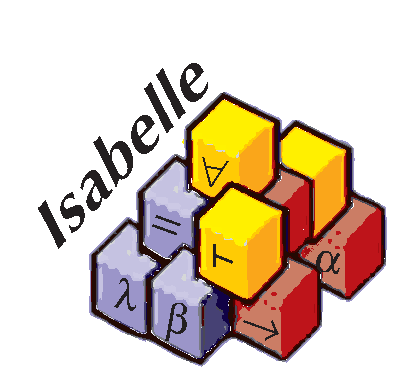
\includegraphics[scale=0.5]{isabelle.eps} \\[4ex] Isabelle's Object-Logics}

\author{{\em Lawrence C. Paulson}\\
        Computer Laboratory \\ University of Cambridge \\
        \texttt{lcp@cl.cam.ac.uk}\\[3ex] 
        With Contributions by Tobias Nipkow and Markus Wenzel%
\thanks{Tobias Nipkow revised and extended
    the chapter on \HOL.  Markus Wenzel made numerous improvements.
    Philippe de Groote wrote the
    first version of the logic~\LK{} and contributed to~\ZF{}.  Tobias
    Nipkow developed~\HOL{}, \LCF{} and~\Cube{}.  Philippe No\"el and
    Martin Coen made many contributions to~\ZF{}.  Martin Coen
    developed~\Modal{} with assistance from Rajeev Gor\'e.  The research has 
    been funded by the EPSRC (grants GR/G53279, GR/H40570, GR/K57381,
    GR/K77051) and by ESPRIT project 6453: Types.}
}

\newcommand\subcaption[1]{\par {\centering\normalsize\sc#1\par}\bigskip
  \hrule\bigskip}
\newenvironment{constants}{\begin{center}\small\begin{tabular}{rrrr}}{\end{tabular}\end{center}}

\makeindex

%%\newenvironment{example}{\begin{Example}\rm}{\end{Example}}
%%\newtheorem{Example}{Example}[chapter]

\underscoreoff

\setcounter{secnumdepth}{2} \setcounter{tocdepth}{2}  %% {secnumdepth}{2}???

\pagestyle{headings}
\sloppy
\binperiod     %%%treat . like a binary operator

\begin{document}
\maketitle 
\pagenumbering{roman} \tableofcontents \clearfirst

\chapter{Introduction}

\section{Quick start}

FIXME examples, ProofGeneral setup

\section{Examples}

\section{How to write Isar proofs anyway?}


%%% Local Variables: 
%%% mode: latex
%%% TeX-master: "isar-ref"
%%% End: 

%% $Id$
\chapter{First-Order Logic}
\index{first-order logic|(}

Isabelle implements Gentzen's natural deduction systems {\sc nj} and {\sc
  nk}.  Intuitionistic first-order logic is defined first, as theory
\thydx{IFOL}.  Classical logic, theory \thydx{FOL}, is
obtained by adding the double negation rule.  Basic proof procedures are
provided.  The intuitionistic prover works with derived rules to simplify
implications in the assumptions.  Classical~\texttt{FOL} employs Isabelle's
classical reasoner, which simulates a sequent calculus.

\section{Syntax and rules of inference}
The logic is many-sorted, using Isabelle's type classes.  The class of
first-order terms is called \cldx{term} and is a subclass of \texttt{logic}.
No types of individuals are provided, but extensions can define types such
as \texttt{nat::term} and type constructors such as \texttt{list::(term)term}
(see the examples directory, \texttt{FOL/ex}).  Below, the type variable
$\alpha$ ranges over class \texttt{term}; the equality symbol and quantifiers
are polymorphic (many-sorted).  The type of formulae is~\tydx{o}, which
belongs to class~\cldx{logic}.  Figure~\ref{fol-syntax} gives the syntax.
Note that $a$\verb|~=|$b$ is translated to $\neg(a=b)$.

Figure~\ref{fol-rules} shows the inference rules with their~\ML\ names.
Negation is defined in the usual way for intuitionistic logic; $\neg P$
abbreviates $P\imp\bot$.  The biconditional~($\bimp$) is defined through
$\conj$ and~$\imp$; introduction and elimination rules are derived for it.

The unique existence quantifier, $\exists!x.P(x)$, is defined in terms
of~$\exists$ and~$\forall$.  An Isabelle binder, it admits nested
quantifications.  For instance, $\exists!x\;y.P(x,y)$ abbreviates
$\exists!x. \exists!y.P(x,y)$; note that this does not mean that there
exists a unique pair $(x,y)$ satisfying~$P(x,y)$.

Some intuitionistic derived rules are shown in
Fig.\ts\ref{fol-int-derived}, again with their \ML\ names.  These include
rules for the defined symbols $\neg$, $\bimp$ and $\exists!$.  Natural
deduction typically involves a combination of forward and backward
reasoning, particularly with the destruction rules $(\conj E)$,
$({\imp}E)$, and~$(\forall E)$.  Isabelle's backward style handles these
rules badly, so sequent-style rules are derived to eliminate conjunctions,
implications, and universal quantifiers.  Used with elim-resolution,
\tdx{allE} eliminates a universal quantifier while \tdx{all_dupE}
re-inserts the quantified formula for later use.  The rules {\tt
conj_impE}, etc., support the intuitionistic proof procedure
(see~\S\ref{fol-int-prover}).

See the files \texttt{FOL/IFOL.thy}, \texttt{FOL/IFOL.ML} and
\texttt{FOL/intprover.ML} for complete listings of the rules and
derived rules.

\begin{figure} 
\begin{center}
\begin{tabular}{rrr} 
  \it name      &\it meta-type  & \it description \\ 
  \cdx{Trueprop}& $o\To prop$           & coercion to $prop$\\
  \cdx{Not}     & $o\To o$              & negation ($\neg$) \\
  \cdx{True}    & $o$                   & tautology ($\top$) \\
  \cdx{False}   & $o$                   & absurdity ($\bot$)
\end{tabular}
\end{center}
\subcaption{Constants}

\begin{center}
\begin{tabular}{llrrr} 
  \it symbol &\it name     &\it meta-type & \it priority & \it description \\
  \sdx{ALL}  & \cdx{All}  & $(\alpha\To o)\To o$ & 10 & 
        universal quantifier ($\forall$) \\
  \sdx{EX}   & \cdx{Ex}   & $(\alpha\To o)\To o$ & 10 & 
        existential quantifier ($\exists$) \\
  \texttt{EX!}  & \cdx{Ex1}  & $(\alpha\To o)\To o$ & 10 & 
        unique existence ($\exists!$)
\end{tabular}
\index{*"E"X"! symbol}
\end{center}
\subcaption{Binders} 

\begin{center}
\index{*"= symbol}
\index{&@{\tt\&} symbol}
\index{*"| symbol}
\index{*"-"-"> symbol}
\index{*"<"-"> symbol}
\begin{tabular}{rrrr} 
  \it symbol    & \it meta-type         & \it priority & \it description \\ 
  \tt =         & $[\alpha,\alpha]\To o$ & Left 50 & equality ($=$) \\
  \tt \&        & $[o,o]\To o$          & Right 35 & conjunction ($\conj$) \\
  \tt |         & $[o,o]\To o$          & Right 30 & disjunction ($\disj$) \\
  \tt -->       & $[o,o]\To o$          & Right 25 & implication ($\imp$) \\
  \tt <->       & $[o,o]\To o$          & Right 25 & biconditional ($\bimp$) 
\end{tabular}
\end{center}
\subcaption{Infixes}

\dquotes
\[\begin{array}{rcl}
 formula & = & \hbox{expression of type~$o$} \\
         & | & term " = " term \quad| \quad term " \ttilde= " term \\
         & | & "\ttilde\ " formula \\
         & | & formula " \& " formula \\
         & | & formula " | " formula \\
         & | & formula " --> " formula \\
         & | & formula " <-> " formula \\
         & | & "ALL~" id~id^* " . " formula \\
         & | & "EX~~" id~id^* " . " formula \\
         & | & "EX!~" id~id^* " . " formula
  \end{array}
\]
\subcaption{Grammar}
\caption{Syntax of \texttt{FOL}} \label{fol-syntax}
\end{figure}


\begin{figure} 
\begin{ttbox}
\tdx{refl}        a=a
\tdx{subst}       [| a=b;  P(a) |] ==> P(b)
\subcaption{Equality rules}

\tdx{conjI}       [| P;  Q |] ==> P&Q
\tdx{conjunct1}   P&Q ==> P
\tdx{conjunct2}   P&Q ==> Q

\tdx{disjI1}      P ==> P|Q
\tdx{disjI2}      Q ==> P|Q
\tdx{disjE}       [| P|Q;  P ==> R;  Q ==> R |] ==> R

\tdx{impI}        (P ==> Q) ==> P-->Q
\tdx{mp}          [| P-->Q;  P |] ==> Q

\tdx{FalseE}      False ==> P
\subcaption{Propositional rules}

\tdx{allI}        (!!x. P(x))  ==> (ALL x.P(x))
\tdx{spec}        (ALL x.P(x)) ==> P(x)

\tdx{exI}         P(x) ==> (EX x.P(x))
\tdx{exE}         [| EX x.P(x);  !!x. P(x) ==> R |] ==> R
\subcaption{Quantifier rules}

\tdx{True_def}    True        == False-->False
\tdx{not_def}     ~P          == P-->False
\tdx{iff_def}     P<->Q       == (P-->Q) & (Q-->P)
\tdx{ex1_def}     EX! x. P(x) == EX x. P(x) & (ALL y. P(y) --> y=x)
\subcaption{Definitions}
\end{ttbox}

\caption{Rules of intuitionistic logic} \label{fol-rules}
\end{figure}


\begin{figure} 
\begin{ttbox}
\tdx{sym}       a=b ==> b=a
\tdx{trans}     [| a=b;  b=c |] ==> a=c
\tdx{ssubst}    [| b=a;  P(a) |] ==> P(b)
\subcaption{Derived equality rules}

\tdx{TrueI}     True

\tdx{notI}      (P ==> False) ==> ~P
\tdx{notE}      [| ~P;  P |] ==> R

\tdx{iffI}      [| P ==> Q;  Q ==> P |] ==> P<->Q
\tdx{iffE}      [| P <-> Q;  [| P-->Q; Q-->P |] ==> R |] ==> R
\tdx{iffD1}     [| P <-> Q;  P |] ==> Q            
\tdx{iffD2}     [| P <-> Q;  Q |] ==> P

\tdx{ex1I}      [| P(a);  !!x. P(x) ==> x=a |]  ==>  EX! x. P(x)
\tdx{ex1E}      [| EX! x.P(x);  !!x.[| P(x);  ALL y. P(y) --> y=x |] ==> R 
          |] ==> R
\subcaption{Derived rules for \(\top\), \(\neg\), \(\bimp\) and \(\exists!\)}

\tdx{conjE}     [| P&Q;  [| P; Q |] ==> R |] ==> R
\tdx{impE}      [| P-->Q;  P;  Q ==> R |] ==> R
\tdx{allE}      [| ALL x.P(x);  P(x) ==> R |] ==> R
\tdx{all_dupE}  [| ALL x.P(x);  [| P(x); ALL x.P(x) |] ==> R |] ==> R
\subcaption{Sequent-style elimination rules}

\tdx{conj_impE} [| (P&Q)-->S;  P-->(Q-->S) ==> R |] ==> R
\tdx{disj_impE} [| (P|Q)-->S;  [| P-->S; Q-->S |] ==> R |] ==> R
\tdx{imp_impE}  [| (P-->Q)-->S;  [| P; Q-->S |] ==> Q;  S ==> R |] ==> R
\tdx{not_impE}  [| ~P --> S;  P ==> False;  S ==> R |] ==> R
\tdx{iff_impE}  [| (P<->Q)-->S; [| P; Q-->S |] ==> Q; [| Q; P-->S |] ==> P;
             S ==> R |] ==> R
\tdx{all_impE}  [| (ALL x.P(x))-->S;  !!x.P(x);  S ==> R |] ==> R
\tdx{ex_impE}   [| (EX x.P(x))-->S;  P(a)-->S ==> R |] ==> R
\end{ttbox}
\subcaption{Intuitionistic simplification of implication}
\caption{Derived rules for intuitionistic logic} \label{fol-int-derived}
\end{figure}


\section{Generic packages}
FOL instantiates most of Isabelle's generic packages.
\begin{itemize}
\item 
It instantiates the simplifier.  Both equality ($=$) and the biconditional
($\bimp$) may be used for rewriting.  Tactics such as \texttt{Asm_simp_tac} and
\texttt{Full_simp_tac} refer to the default simpset (\texttt{simpset()}), which works for
most purposes.  Named simplification sets include \ttindexbold{IFOL_ss},
for intuitionistic first-order logic, and \ttindexbold{FOL_ss},
for classical logic.  See the file
\texttt{FOL/simpdata.ML} for a complete listing of the simplification
rules%
\iflabelundefined{sec:setting-up-simp}{}%
        {, and \S\ref{sec:setting-up-simp} for discussion}.

\item 
It instantiates the classical reasoner.  See~\S\ref{fol-cla-prover}
for details. 

\item FOL provides the tactic \ttindex{hyp_subst_tac}, which substitutes for
  an equality throughout a subgoal and its hypotheses.  This tactic uses FOL's
  general substitution rule.
\end{itemize}

\begin{warn}\index{simplification!of conjunctions}%
  Reducing $a=b\conj P(a)$ to $a=b\conj P(b)$ is sometimes advantageous.  The
  left part of a conjunction helps in simplifying the right part.  This effect
  is not available by default: it can be slow.  It can be obtained by
  including \ttindex{conj_cong} in a simpset, \verb$addcongs [conj_cong]$.
\end{warn}


\section{Intuitionistic proof procedures} \label{fol-int-prover}
Implication elimination (the rules~\texttt{mp} and~\texttt{impE}) pose
difficulties for automated proof.  In intuitionistic logic, the assumption
$P\imp Q$ cannot be treated like $\neg P\disj Q$.  Given $P\imp Q$, we may
use~$Q$ provided we can prove~$P$; the proof of~$P$ may require repeated
use of $P\imp Q$.  If the proof of~$P$ fails then the whole branch of the
proof must be abandoned.  Thus intuitionistic propositional logic requires
backtracking.  

For an elementary example, consider the intuitionistic proof of $Q$ from
$P\imp Q$ and $(P\imp Q)\imp P$.  The implication $P\imp Q$ is needed
twice:
\[ \infer[({\imp}E)]{Q}{P\imp Q &
       \infer[({\imp}E)]{P}{(P\imp Q)\imp P & P\imp Q}} 
\]
The theorem prover for intuitionistic logic does not use~\texttt{impE}.\@
Instead, it simplifies implications using derived rules
(Fig.\ts\ref{fol-int-derived}).  It reduces the antecedents of implications
to atoms and then uses Modus Ponens: from $P\imp Q$ and~$P$ deduce~$Q$.
The rules \tdx{conj_impE} and \tdx{disj_impE} are 
straightforward: $(P\conj Q)\imp S$ is equivalent to $P\imp (Q\imp S)$, and
$(P\disj Q)\imp S$ is equivalent to the conjunction of $P\imp S$ and $Q\imp
S$.  The other \ldots{\tt_impE} rules are unsafe; the method requires
backtracking.  All the rules are derived in the same simple manner.

Dyckhoff has independently discovered similar rules, and (more importantly)
has demonstrated their completeness for propositional
logic~\cite{dyckhoff}.  However, the tactics given below are not complete
for first-order logic because they discard universally quantified
assumptions after a single use.
\begin{ttbox} 
mp_tac              : int -> tactic
eq_mp_tac           : int -> tactic
IntPr.safe_step_tac : int -> tactic
IntPr.safe_tac      :        tactic
IntPr.inst_step_tac : int -> tactic
IntPr.step_tac      : int -> tactic
IntPr.fast_tac      : int -> tactic
IntPr.best_tac      : int -> tactic
\end{ttbox}
Most of these belong to the structure \texttt{IntPr} and resemble the
tactics of Isabelle's classical reasoner.

\begin{ttdescription}
\item[\ttindexbold{mp_tac} {\it i}] 
attempts to use \tdx{notE} or \tdx{impE} within the assumptions in
subgoal $i$.  For each assumption of the form $\neg P$ or $P\imp Q$, it
searches for another assumption unifiable with~$P$.  By
contradiction with $\neg P$ it can solve the subgoal completely; by Modus
Ponens it can replace the assumption $P\imp Q$ by $Q$.  The tactic can
produce multiple outcomes, enumerating all suitable pairs of assumptions.

\item[\ttindexbold{eq_mp_tac} {\it i}] 
is like \texttt{mp_tac} {\it i}, but may not instantiate unknowns --- thus, it
is safe.

\item[\ttindexbold{IntPr.safe_step_tac} $i$] performs a safe step on
subgoal~$i$.  This may include proof by assumption or Modus Ponens (taking
care not to instantiate unknowns), or \texttt{hyp_subst_tac}. 

\item[\ttindexbold{IntPr.safe_tac}] repeatedly performs safe steps on all 
subgoals.  It is deterministic, with at most one outcome.

\item[\ttindexbold{IntPr.inst_step_tac} $i$] is like \texttt{safe_step_tac},
but allows unknowns to be instantiated.

\item[\ttindexbold{IntPr.step_tac} $i$] tries \texttt{safe_tac} or {\tt
    inst_step_tac}, or applies an unsafe rule.  This is the basic step of
  the intuitionistic proof procedure.

\item[\ttindexbold{IntPr.fast_tac} $i$] applies \texttt{step_tac}, using
depth-first search, to solve subgoal~$i$.

\item[\ttindexbold{IntPr.best_tac} $i$] applies \texttt{step_tac}, using
best-first search (guided by the size of the proof state) to solve subgoal~$i$.
\end{ttdescription}
Here are some of the theorems that \texttt{IntPr.fast_tac} proves
automatically.  The latter three date from {\it Principia Mathematica}
(*11.53, *11.55, *11.61)~\cite{principia}.
\begin{ttbox}
~~P & ~~(P --> Q) --> ~~Q
(ALL x y. P(x) --> Q(y)) <-> ((EX x. P(x)) --> (ALL y. Q(y)))
(EX x y. P(x) & Q(x,y)) <-> (EX x. P(x) & (EX y. Q(x,y)))
(EX y. ALL x. P(x) --> Q(x,y)) --> (ALL x. P(x) --> (EX y. Q(x,y)))
\end{ttbox}



\begin{figure} 
\begin{ttbox}
\tdx{excluded_middle}    ~P | P

\tdx{disjCI}    (~Q ==> P) ==> P|Q
\tdx{exCI}      (ALL x. ~P(x) ==> P(a)) ==> EX x.P(x)
\tdx{impCE}     [| P-->Q; ~P ==> R; Q ==> R |] ==> R
\tdx{iffCE}     [| P<->Q;  [| P; Q |] ==> R;  [| ~P; ~Q |] ==> R |] ==> R
\tdx{notnotD}   ~~P ==> P
\tdx{swap}      ~P ==> (~Q ==> P) ==> Q
\end{ttbox}
\caption{Derived rules for classical logic} \label{fol-cla-derived}
\end{figure}


\section{Classical proof procedures} \label{fol-cla-prover}
The classical theory, \thydx{FOL}, consists of intuitionistic logic plus
the rule
$$ \vcenter{\infer{P}{\infer*{P}{[\neg P]}}} \eqno(classical) $$
\noindent
Natural deduction in classical logic is not really all that natural.  FOL
derives classical introduction rules for $\disj$ and~$\exists$, as well as
classical elimination rules for~$\imp$ and~$\bimp$, and the swap rule (see
Fig.\ts\ref{fol-cla-derived}).

The classical reasoner is installed.  Tactics such as \texttt{Blast_tac} and {\tt
Best_tac} refer to the default claset (\texttt{claset()}), which works for most
purposes.  Named clasets include \ttindexbold{prop_cs}, which includes the
propositional rules, and \ttindexbold{FOL_cs}, which also includes quantifier
rules.  See the file \texttt{FOL/cladata.ML} for lists of the
classical rules, and 
\iflabelundefined{chap:classical}{the {\em Reference Manual\/}}%
        {Chap.\ts\ref{chap:classical}} 
for more discussion of classical proof methods.


\section{An intuitionistic example}
Here is a session similar to one in {\em Logic and Computation}
\cite[pages~222--3]{paulson87}.  Isabelle treats quantifiers differently
from {\sc lcf}-based theorem provers such as {\sc hol}.  

First, we specify that we are working in intuitionistic logic:
\begin{ttbox}
context IFOL.thy;
\end{ttbox}
The proof begins by entering the goal, then applying the rule $({\imp}I)$.
\begin{ttbox}
Goal "(EX y. ALL x. Q(x,y)) -->  (ALL x. EX y. Q(x,y))";
{\out Level 0}
{\out (EX y. ALL x. Q(x,y)) --> (ALL x. EX y. Q(x,y))}
{\out  1. (EX y. ALL x. Q(x,y)) --> (ALL x. EX y. Q(x,y))}
\ttbreak
by (resolve_tac [impI] 1);
{\out Level 1}
{\out (EX y. ALL x. Q(x,y)) --> (ALL x. EX y. Q(x,y))}
{\out  1. EX y. ALL x. Q(x,y) ==> ALL x. EX y. Q(x,y)}
\end{ttbox}
In this example, we shall never have more than one subgoal.  Applying
$({\imp}I)$ replaces~\verb|-->| by~\verb|==>|, making
\(\ex{y}\all{x}Q(x,y)\) an assumption.  We have the choice of
$({\exists}E)$ and $({\forall}I)$; let us try the latter.
\begin{ttbox}
by (resolve_tac [allI] 1);
{\out Level 2}
{\out (EX y. ALL x. Q(x,y)) --> (ALL x. EX y. Q(x,y))}
{\out  1. !!x. EX y. ALL x. Q(x,y) ==> EX y. Q(x,y)}
\end{ttbox}
Applying $({\forall}I)$ replaces the \texttt{ALL~x} by \hbox{\tt!!x},
changing the universal quantifier from object~($\forall$) to
meta~($\Forall$).  The bound variable is a {\bf parameter} of the
subgoal.  We now must choose between $({\exists}I)$ and $({\exists}E)$.  What
happens if the wrong rule is chosen?
\begin{ttbox}
by (resolve_tac [exI] 1);
{\out Level 3}
{\out (EX y. ALL x. Q(x,y)) --> (ALL x. EX y. Q(x,y))}
{\out  1. !!x. EX y. ALL x. Q(x,y) ==> Q(x,?y2(x))}
\end{ttbox}
The new subgoal~1 contains the function variable {\tt?y2}.  Instantiating
{\tt?y2} can replace~{\tt?y2(x)} by a term containing~\texttt{x}, even
though~\texttt{x} is a bound variable.  Now we analyse the assumption
\(\exists y.\forall x. Q(x,y)\) using elimination rules:
\begin{ttbox}
by (eresolve_tac [exE] 1);
{\out Level 4}
{\out (EX y. ALL x. Q(x,y)) --> (ALL x. EX y. Q(x,y))}
{\out  1. !!x y. ALL x. Q(x,y) ==> Q(x,?y2(x))}
\end{ttbox}
Applying $(\exists E)$ has produced the parameter \texttt{y} and stripped the
existential quantifier from the assumption.  But the subgoal is unprovable:
there is no way to unify \texttt{?y2(x)} with the bound variable~\texttt{y}.
Using \texttt{choplev} we can return to the critical point.  This time we
apply $({\exists}E)$:
\begin{ttbox}
choplev 2;
{\out Level 2}
{\out (EX y. ALL x. Q(x,y)) --> (ALL x. EX y. Q(x,y))}
{\out  1. !!x. EX y. ALL x. Q(x,y) ==> EX y. Q(x,y)}
\ttbreak
by (eresolve_tac [exE] 1);
{\out Level 3}
{\out (EX y. ALL x. Q(x,y)) --> (ALL x. EX y. Q(x,y))}
{\out  1. !!x y. ALL x. Q(x,y) ==> EX y. Q(x,y)}
\end{ttbox}
We now have two parameters and no scheme variables.  Applying
$({\exists}I)$ and $({\forall}E)$ produces two scheme variables, which are
applied to those parameters.  Parameters should be produced early, as this
example demonstrates.
\begin{ttbox}
by (resolve_tac [exI] 1);
{\out Level 4}
{\out (EX y. ALL x. Q(x,y)) --> (ALL x. EX y. Q(x,y))}
{\out  1. !!x y. ALL x. Q(x,y) ==> Q(x,?y3(x,y))}
\ttbreak
by (eresolve_tac [allE] 1);
{\out Level 5}
{\out (EX y. ALL x. Q(x,y)) --> (ALL x. EX y. Q(x,y))}
{\out  1. !!x y. Q(?x4(x,y),y) ==> Q(x,?y3(x,y))}
\end{ttbox}
The subgoal has variables \texttt{?y3} and \texttt{?x4} applied to both
parameters.  The obvious projection functions unify {\tt?x4(x,y)} with~{\tt
x} and \verb|?y3(x,y)| with~\texttt{y}.
\begin{ttbox}
by (assume_tac 1);
{\out Level 6}
{\out (EX y. ALL x. Q(x,y)) --> (ALL x. EX y. Q(x,y))}
{\out No subgoals!}
\end{ttbox}
The theorem was proved in six tactic steps, not counting the abandoned
ones.  But proof checking is tedious; \ttindex{IntPr.fast_tac} proves the
theorem in one step.
\begin{ttbox}
Goal "(EX y. ALL x. Q(x,y)) -->  (ALL x. EX y. Q(x,y))";
{\out Level 0}
{\out (EX y. ALL x. Q(x,y)) --> (ALL x. EX y. Q(x,y))}
{\out  1. (EX y. ALL x. Q(x,y)) --> (ALL x. EX y. Q(x,y))}
by (IntPr.fast_tac 1);
{\out Level 1}
{\out (EX y. ALL x. Q(x,y)) --> (ALL x. EX y. Q(x,y))}
{\out No subgoals!}
\end{ttbox}


\section{An example of intuitionistic negation}
The following example demonstrates the specialized forms of implication
elimination.  Even propositional formulae can be difficult to prove from
the basic rules; the specialized rules help considerably.  

Propositional examples are easy to invent.  As Dummett notes~\cite[page
28]{dummett}, $\neg P$ is classically provable if and only if it is
intuitionistically provable;  therefore, $P$ is classically provable if and
only if $\neg\neg P$ is intuitionistically provable.%
\footnote{Of course this holds only for propositional logic, not if $P$ is
  allowed to contain quantifiers.} Proving $\neg\neg P$ intuitionistically is
much harder than proving~$P$ classically.

Our example is the double negation of the classical tautology $(P\imp
Q)\disj (Q\imp P)$.  When stating the goal, we command Isabelle to expand
negations to implications using the definition $\neg P\equiv P\imp\bot$.
This allows use of the special implication rules.
\begin{ttbox}
Goalw [not_def] "~ ~ ((P-->Q) | (Q-->P))";
{\out Level 0}
{\out ~ ~ ((P --> Q) | (Q --> P))}
{\out  1. ((P --> Q) | (Q --> P) --> False) --> False}
\end{ttbox}
The first step is trivial.
\begin{ttbox}
by (resolve_tac [impI] 1);
{\out Level 1}
{\out ~ ~ ((P --> Q) | (Q --> P))}
{\out  1. (P --> Q) | (Q --> P) --> False ==> False}
\end{ttbox}
By $(\imp E)$ it would suffice to prove $(P\imp Q)\disj (Q\imp P)$, but
that formula is not a theorem of intuitionistic logic.  Instead we apply
the specialized implication rule \tdx{disj_impE}.  It splits the
assumption into two assumptions, one for each disjunct.
\begin{ttbox}
by (eresolve_tac [disj_impE] 1);
{\out Level 2}
{\out ~ ~ ((P --> Q) | (Q --> P))}
{\out  1. [| (P --> Q) --> False; (Q --> P) --> False |] ==> False}
\end{ttbox}
We cannot hope to prove $P\imp Q$ or $Q\imp P$ separately, but
their negations are inconsistent.  Applying \tdx{imp_impE} breaks down
the assumption $\neg(P\imp Q)$, asking to show~$Q$ while providing new
assumptions~$P$ and~$\neg Q$.
\begin{ttbox}
by (eresolve_tac [imp_impE] 1);
{\out Level 3}
{\out ~ ~ ((P --> Q) | (Q --> P))}
{\out  1. [| (Q --> P) --> False; P; Q --> False |] ==> Q}
{\out  2. [| (Q --> P) --> False; False |] ==> False}
\end{ttbox}
Subgoal~2 holds trivially; let us ignore it and continue working on
subgoal~1.  Thanks to the assumption~$P$, we could prove $Q\imp P$;
applying \tdx{imp_impE} is simpler.
\begin{ttbox}
by (eresolve_tac [imp_impE] 1);
{\out Level 4}
{\out ~ ~ ((P --> Q) | (Q --> P))}
{\out  1. [| P; Q --> False; Q; P --> False |] ==> P}
{\out  2. [| P; Q --> False; False |] ==> Q}
{\out  3. [| (Q --> P) --> False; False |] ==> False}
\end{ttbox}
The three subgoals are all trivial.
\begin{ttbox}
by (REPEAT (eresolve_tac [FalseE] 2));
{\out Level 5}
{\out ~ ~ ((P --> Q) | (Q --> P))}
{\out  1. [| P; Q --> False; Q; P --> False |] ==> P}
\ttbreak
by (assume_tac 1);
{\out Level 6}
{\out ~ ~ ((P --> Q) | (Q --> P))}
{\out No subgoals!}
\end{ttbox}
This proof is also trivial for \texttt{IntPr.fast_tac}.


\section{A classical example} \label{fol-cla-example}
To illustrate classical logic, we shall prove the theorem
$\ex{y}\all{x}P(y)\imp P(x)$.  Informally, the theorem can be proved as
follows.  Choose~$y$ such that~$\neg P(y)$, if such exists; otherwise
$\all{x}P(x)$ is true.  Either way the theorem holds.  First, we switch to
classical logic:
\begin{ttbox}
context FOL.thy;
\end{ttbox}

The formal proof does not conform in any obvious way to the sketch given
above.  The key inference is the first one, \tdx{exCI}; this classical
version of~$(\exists I)$ allows multiple instantiation of the quantifier.
\begin{ttbox}
Goal "EX y. ALL x. P(y)-->P(x)";
{\out Level 0}
{\out EX y. ALL x. P(y) --> P(x)}
{\out  1. EX y. ALL x. P(y) --> P(x)}
\ttbreak
by (resolve_tac [exCI] 1);
{\out Level 1}
{\out EX y. ALL x. P(y) --> P(x)}
{\out  1. ALL y. ~ (ALL x. P(y) --> P(x)) ==> ALL x. P(?a) --> P(x)}
\end{ttbox}
We can either exhibit a term {\tt?a} to satisfy the conclusion of
subgoal~1, or produce a contradiction from the assumption.  The next
steps are routine.
\begin{ttbox}
by (resolve_tac [allI] 1);
{\out Level 2}
{\out EX y. ALL x. P(y) --> P(x)}
{\out  1. !!x. ALL y. ~ (ALL x. P(y) --> P(x)) ==> P(?a) --> P(x)}
\ttbreak
by (resolve_tac [impI] 1);
{\out Level 3}
{\out EX y. ALL x. P(y) --> P(x)}
{\out  1. !!x. [| ALL y. ~ (ALL x. P(y) --> P(x)); P(?a) |] ==> P(x)}
\end{ttbox}
By the duality between $\exists$ and~$\forall$, applying~$(\forall E)$
in effect applies~$(\exists I)$ again.
\begin{ttbox}
by (eresolve_tac [allE] 1);
{\out Level 4}
{\out EX y. ALL x. P(y) --> P(x)}
{\out  1. !!x. [| P(?a); ~ (ALL xa. P(?y3(x)) --> P(xa)) |] ==> P(x)}
\end{ttbox}
In classical logic, a negated assumption is equivalent to a conclusion.  To
get this effect, we create a swapped version of $(\forall I)$ and apply it
using \ttindex{eresolve_tac}; we could equivalently have applied $(\forall
I)$ using \ttindex{swap_res_tac}.
\begin{ttbox}
allI RSN (2,swap);
{\out val it = "[| ~(ALL x. ?P1(x)); !!x. ~ ?Q ==> ?P1(x) |] ==> ?Q" : thm}
by (eresolve_tac [it] 1);
{\out Level 5}
{\out EX y. ALL x. P(y) --> P(x)}
{\out  1. !!x xa. [| P(?a); ~ P(x) |] ==> P(?y3(x)) --> P(xa)}
\end{ttbox}
The previous conclusion, \texttt{P(x)}, has become a negated assumption.
\begin{ttbox}
by (resolve_tac [impI] 1);
{\out Level 6}
{\out EX y. ALL x. P(y) --> P(x)}
{\out  1. !!x xa. [| P(?a); ~ P(x); P(?y3(x)) |] ==> P(xa)}
\end{ttbox}
The subgoal has three assumptions.  We produce a contradiction between the
\index{assumptions!contradictory} assumptions~\verb|~P(x)| and~{\tt
  P(?y3(x))}.  The proof never instantiates the unknown~{\tt?a}.
\begin{ttbox}
by (eresolve_tac [notE] 1);
{\out Level 7}
{\out EX y. ALL x. P(y) --> P(x)}
{\out  1. !!x xa. [| P(?a); P(?y3(x)) |] ==> P(x)}
\ttbreak
by (assume_tac 1);
{\out Level 8}
{\out EX y. ALL x. P(y) --> P(x)}
{\out No subgoals!}
\end{ttbox}
The civilised way to prove this theorem is through \ttindex{Blast_tac},
which automatically uses the classical version of~$(\exists I)$:
\begin{ttbox}
Goal "EX y. ALL x. P(y)-->P(x)";
{\out Level 0}
{\out EX y. ALL x. P(y) --> P(x)}
{\out  1. EX y. ALL x. P(y) --> P(x)}
by (Blast_tac 1);
{\out Depth = 0}
{\out Depth = 1}
{\out Depth = 2}
{\out Level 1}
{\out EX y. ALL x. P(y) --> P(x)}
{\out No subgoals!}
\end{ttbox}
If this theorem seems counterintuitive, then perhaps you are an
intuitionist.  In constructive logic, proving $\ex{y}\all{x}P(y)\imp P(x)$
requires exhibiting a particular term~$t$ such that $\all{x}P(t)\imp P(x)$,
which we cannot do without further knowledge about~$P$.


\section{Derived rules and the classical tactics}
Classical first-order logic can be extended with the propositional
connective $if(P,Q,R)$, where 
$$ if(P,Q,R) \equiv P\conj Q \disj \neg P \conj R. \eqno(if) $$
Theorems about $if$ can be proved by treating this as an abbreviation,
replacing $if(P,Q,R)$ by $P\conj Q \disj \neg P \conj R$ in subgoals.  But
this duplicates~$P$, causing an exponential blowup and an unreadable
formula.  Introducing further abbreviations makes the problem worse.

Natural deduction demands rules that introduce and eliminate $if(P,Q,R)$
directly, without reference to its definition.  The simple identity
\[ if(P,Q,R) \,\bimp\, (P\imp Q)\conj (\neg P\imp R) \]
suggests that the
$if$-introduction rule should be
\[ \infer[({if}\,I)]{if(P,Q,R)}{\infer*{Q}{[P]}  &  \infer*{R}{[\neg P]}} \]
The $if$-elimination rule reflects the definition of $if(P,Q,R)$ and the
elimination rules for~$\disj$ and~$\conj$.
\[ \infer[({if}\,E)]{S}{if(P,Q,R) & \infer*{S}{[P,Q]}
                                  & \infer*{S}{[\neg P,R]}} 
\]
Having made these plans, we get down to work with Isabelle.  The theory of
classical logic, \texttt{FOL}, is extended with the constant
$if::[o,o,o]\To o$.  The axiom \tdx{if_def} asserts the
equation~$(if)$.
\begin{ttbox}
If = FOL +
consts  if     :: [o,o,o]=>o
rules   if_def "if(P,Q,R) == P&Q | ~P&R"
end
\end{ttbox}
We create the file \texttt{If.thy} containing these declarations.  (This file
is on directory \texttt{FOL/ex} in the Isabelle distribution.)  Typing
\begin{ttbox}
use_thy "If";  
\end{ttbox}
loads that theory and sets it to be the current context.


\subsection{Deriving the introduction rule}

The derivations of the introduction and elimination rules demonstrate the
methods for rewriting with definitions.  Classical reasoning is required,
so we use \texttt{blast_tac}.

The introduction rule, given the premises $P\Imp Q$ and $\neg P\Imp R$,
concludes $if(P,Q,R)$.  We propose the conclusion as the main goal
using~\ttindex{Goalw}, which uses \texttt{if_def} to rewrite occurrences
of $if$ in the subgoal.
\begin{ttbox}
val prems = Goalw [if_def]
    "[| P ==> Q; ~ P ==> R |] ==> if(P,Q,R)";
{\out Level 0}
{\out if(P,Q,R)}
{\out  1. P & Q | ~ P & R}
\end{ttbox}
The premises (bound to the {\ML} variable \texttt{prems}) are passed as
introduction rules to \ttindex{blast_tac}.  Remember that \texttt{claset()} refers
to the default classical set.
\begin{ttbox}
by (blast_tac (claset() addIs prems) 1);
{\out Level 1}
{\out if(P,Q,R)}
{\out No subgoals!}
qed "ifI";
\end{ttbox}


\subsection{Deriving the elimination rule}
The elimination rule has three premises, two of which are themselves rules.
The conclusion is simply $S$.
\begin{ttbox}
val major::prems = Goalw [if_def]
   "[| if(P,Q,R);  [| P; Q |] ==> S; [| ~ P; R |] ==> S |] ==> S";
{\out Level 0}
{\out S}
{\out  1. S}
\end{ttbox}
The major premise contains an occurrence of~$if$, but the version returned
by \ttindex{Goalw} (and bound to the {\ML} variable~\texttt{major}) has the
definition expanded.  Now \ttindex{cut_facts_tac} inserts~\texttt{major} as an
assumption in the subgoal, so that \ttindex{blast_tac} can break it down.
\begin{ttbox}
by (cut_facts_tac [major] 1);
{\out Level 1}
{\out S}
{\out  1. P & Q | ~ P & R ==> S}
\ttbreak
by (blast_tac (claset() addIs prems) 1);
{\out Level 2}
{\out S}
{\out No subgoals!}
qed "ifE";
\end{ttbox}
As you may recall from
\iflabelundefined{definitions}{{\em Introduction to Isabelle}}%
        {\S\ref{definitions}}, there are other
ways of treating definitions when deriving a rule.  We can start the
proof using \texttt{Goal}, which does not expand definitions, instead of
\texttt{Goalw}.  We can use \ttindex{rew_tac}
to expand definitions in the subgoals---perhaps after calling
\ttindex{cut_facts_tac} to insert the rule's premises.  We can use
\ttindex{rewrite_rule}, which is a meta-inference rule, to expand
definitions in the premises directly.


\subsection{Using the derived rules}
The rules just derived have been saved with the {\ML} names \tdx{ifI}
and~\tdx{ifE}.  They permit natural proofs of theorems such as the
following:
\begin{eqnarray*}
    if(P, if(Q,A,B), if(Q,C,D)) & \bimp & if(Q,if(P,A,C),if(P,B,D)) \\
    if(if(P,Q,R), A, B)         & \bimp & if(P,if(Q,A,B),if(R,A,B))
\end{eqnarray*}
Proofs also require the classical reasoning rules and the $\bimp$
introduction rule (called~\tdx{iffI}: do not confuse with~\texttt{ifI}). 

To display the $if$-rules in action, let us analyse a proof step by step.
\begin{ttbox}
Goal "if(P, if(Q,A,B), if(Q,C,D)) <-> if(Q, if(P,A,C), if(P,B,D))";
{\out Level 0}
{\out if(P,if(Q,A,B),if(Q,C,D)) <-> if(Q,if(P,A,C),if(P,B,D))}
{\out  1. if(P,if(Q,A,B),if(Q,C,D)) <-> if(Q,if(P,A,C),if(P,B,D))}
\ttbreak
by (resolve_tac [iffI] 1);
{\out Level 1}
{\out if(P,if(Q,A,B),if(Q,C,D)) <-> if(Q,if(P,A,C),if(P,B,D))}
{\out  1. if(P,if(Q,A,B),if(Q,C,D)) ==> if(Q,if(P,A,C),if(P,B,D))}
{\out  2. if(Q,if(P,A,C),if(P,B,D)) ==> if(P,if(Q,A,B),if(Q,C,D))}
\end{ttbox}
The $if$-elimination rule can be applied twice in succession.
\begin{ttbox}
by (eresolve_tac [ifE] 1);
{\out Level 2}
{\out if(P,if(Q,A,B),if(Q,C,D)) <-> if(Q,if(P,A,C),if(P,B,D))}
{\out  1. [| P; if(Q,A,B) |] ==> if(Q,if(P,A,C),if(P,B,D))}
{\out  2. [| ~ P; if(Q,C,D) |] ==> if(Q,if(P,A,C),if(P,B,D))}
{\out  3. if(Q,if(P,A,C),if(P,B,D)) ==> if(P,if(Q,A,B),if(Q,C,D))}
\ttbreak
by (eresolve_tac [ifE] 1);
{\out Level 3}
{\out if(P,if(Q,A,B),if(Q,C,D)) <-> if(Q,if(P,A,C),if(P,B,D))}
{\out  1. [| P; Q; A |] ==> if(Q,if(P,A,C),if(P,B,D))}
{\out  2. [| P; ~ Q; B |] ==> if(Q,if(P,A,C),if(P,B,D))}
{\out  3. [| ~ P; if(Q,C,D) |] ==> if(Q,if(P,A,C),if(P,B,D))}
{\out  4. if(Q,if(P,A,C),if(P,B,D)) ==> if(P,if(Q,A,B),if(Q,C,D))}
\end{ttbox}
%
In the first two subgoals, all assumptions have been reduced to atoms.  Now
$if$-introduction can be applied.  Observe how the $if$-rules break down
occurrences of $if$ when they become the outermost connective.
\begin{ttbox}
by (resolve_tac [ifI] 1);
{\out Level 4}
{\out if(P,if(Q,A,B),if(Q,C,D)) <-> if(Q,if(P,A,C),if(P,B,D))}
{\out  1. [| P; Q; A; Q |] ==> if(P,A,C)}
{\out  2. [| P; Q; A; ~ Q |] ==> if(P,B,D)}
{\out  3. [| P; ~ Q; B |] ==> if(Q,if(P,A,C),if(P,B,D))}
{\out  4. [| ~ P; if(Q,C,D) |] ==> if(Q,if(P,A,C),if(P,B,D))}
{\out  5. if(Q,if(P,A,C),if(P,B,D)) ==> if(P,if(Q,A,B),if(Q,C,D))}
\ttbreak
by (resolve_tac [ifI] 1);
{\out Level 5}
{\out if(P,if(Q,A,B),if(Q,C,D)) <-> if(Q,if(P,A,C),if(P,B,D))}
{\out  1. [| P; Q; A; Q; P |] ==> A}
{\out  2. [| P; Q; A; Q; ~ P |] ==> C}
{\out  3. [| P; Q; A; ~ Q |] ==> if(P,B,D)}
{\out  4. [| P; ~ Q; B |] ==> if(Q,if(P,A,C),if(P,B,D))}
{\out  5. [| ~ P; if(Q,C,D) |] ==> if(Q,if(P,A,C),if(P,B,D))}
{\out  6. if(Q,if(P,A,C),if(P,B,D)) ==> if(P,if(Q,A,B),if(Q,C,D))}
\end{ttbox}
Where do we stand?  The first subgoal holds by assumption; the second and
third, by contradiction.  This is getting tedious.  We could use the classical
reasoner, but first let us extend the default claset with the derived rules
for~$if$.
\begin{ttbox}
AddSIs [ifI];
AddSEs [ifE];
\end{ttbox}
Now we can revert to the
initial proof state and let \ttindex{blast_tac} solve it.  
\begin{ttbox}
choplev 0;
{\out Level 0}
{\out if(P,if(Q,A,B),if(Q,C,D)) <-> if(Q,if(P,A,C),if(P,B,D))}
{\out  1. if(P,if(Q,A,B),if(Q,C,D)) <-> if(Q,if(P,A,C),if(P,B,D))}
by (Blast_tac 1);
{\out Level 1}
{\out if(P,if(Q,A,B),if(Q,C,D)) <-> if(Q,if(P,A,C),if(P,B,D))}
{\out No subgoals!}
\end{ttbox}
This tactic also solves the other example.
\begin{ttbox}
Goal "if(if(P,Q,R), A, B) <-> if(P, if(Q,A,B), if(R,A,B))";
{\out Level 0}
{\out if(if(P,Q,R),A,B) <-> if(P,if(Q,A,B),if(R,A,B))}
{\out  1. if(if(P,Q,R),A,B) <-> if(P,if(Q,A,B),if(R,A,B))}
\ttbreak
by (Blast_tac 1);
{\out Level 1}
{\out if(if(P,Q,R),A,B) <-> if(P,if(Q,A,B),if(R,A,B))}
{\out No subgoals!}
\end{ttbox}


\subsection{Derived rules versus definitions}
Dispensing with the derived rules, we can treat $if$ as an
abbreviation, and let \ttindex{blast_tac} prove the expanded formula.  Let
us redo the previous proof:
\begin{ttbox}
choplev 0;
{\out Level 0}
{\out if(if(P,Q,R),A,B) <-> if(P,if(Q,A,B),if(R,A,B))}
{\out  1. if(if(P,Q,R),A,B) <-> if(P,if(Q,A,B),if(R,A,B))}
\end{ttbox}
This time, simply unfold using the definition of $if$:
\begin{ttbox}
by (rewtac if_def);
{\out Level 1}
{\out if(if(P,Q,R),A,B) <-> if(P,if(Q,A,B),if(R,A,B))}
{\out  1. (P & Q | ~ P & R) & A | ~ (P & Q | ~ P & R) & B <->}
{\out     P & (Q & A | ~ Q & B) | ~ P & (R & A | ~ R & B)}
\end{ttbox}
We are left with a subgoal in pure first-order logic, which is why the 
classical reasoner can prove it given \texttt{FOL_cs} alone.  (We could, of 
course, have used \texttt{Blast_tac}.)
\begin{ttbox}
by (blast_tac FOL_cs 1);
{\out Level 2}
{\out if(if(P,Q,R),A,B) <-> if(P,if(Q,A,B),if(R,A,B))}
{\out No subgoals!}
\end{ttbox}
Expanding definitions reduces the extended logic to the base logic.  This
approach has its merits --- especially if the prover for the base logic is
good --- but can be slow.  In these examples, proofs using the default
claset (which includes the derived rules) run about six times faster 
than proofs using \texttt{FOL_cs}.

Expanding definitions also complicates error diagnosis.  Suppose we are having
difficulties in proving some goal.  If by expanding definitions we have
made it unreadable, then we have little hope of diagnosing the problem.

Attempts at program verification often yield invalid assertions.
Let us try to prove one:
\begin{ttbox}
Goal "if(if(P,Q,R), A, B) <-> if(P, if(Q,A,B), if(R,B,A))";
{\out Level 0}
{\out if(if(P,Q,R),A,B) <-> if(P,if(Q,A,B),if(R,B,A))}
{\out  1. if(if(P,Q,R),A,B) <-> if(P,if(Q,A,B),if(R,B,A))}
by (Blast_tac 1);
{\out by: tactic failed}
\end{ttbox}
This failure message is uninformative, but we can get a closer look at the
situation by applying \ttindex{Step_tac}.
\begin{ttbox}
by (REPEAT (Step_tac 1));
{\out Level 1}
{\out if(if(P,Q,R),A,B) <-> if(P,if(Q,A,B),if(R,B,A))}
{\out  1. [| A; ~ P; R; ~ P; R |] ==> B}
{\out  2. [| B; ~ P; ~ R; ~ P; ~ R |] ==> A}
{\out  3. [| ~ P; R; B; ~ P; R |] ==> A}
{\out  4. [| ~ P; ~ R; A; ~ B; ~ P |] ==> R}
\end{ttbox}
Subgoal~1 is unprovable and yields a countermodel: $P$ and~$B$ are false
while~$R$ and~$A$ are true.  This truth assignment reduces the main goal to
$true\bimp false$, which is of course invalid.

We can repeat this analysis by expanding definitions, using just the rules of
FOL:
\begin{ttbox}
choplev 0;
{\out Level 0}
{\out if(if(P,Q,R),A,B) <-> if(P,if(Q,A,B),if(R,B,A))}
{\out  1. if(if(P,Q,R),A,B) <-> if(P,if(Q,A,B),if(R,B,A))}
\ttbreak
by (rewtac if_def);
{\out Level 1}
{\out if(if(P,Q,R),A,B) <-> if(P,if(Q,A,B),if(R,B,A))}
{\out  1. (P & Q | ~ P & R) & A | ~ (P & Q | ~ P & R) & B <->}
{\out     P & (Q & A | ~ Q & B) | ~ P & (R & B | ~ R & A)}
by (blast_tac FOL_cs 1);
{\out by: tactic failed}
\end{ttbox}
Again we apply \ttindex{step_tac}:
\begin{ttbox}
by (REPEAT (step_tac FOL_cs 1));
{\out Level 2}
{\out if(if(P,Q,R),A,B) <-> if(P,if(Q,A,B),if(R,B,A))}
{\out  1. [| A; ~ P; R; ~ P; R; ~ False |] ==> B}
{\out  2. [| A; ~ P; R; R; ~ False; ~ B; ~ B |] ==> Q}
{\out  3. [| B; ~ P; ~ R; ~ P; ~ A |] ==> R}
{\out  4. [| B; ~ P; ~ R; ~ Q; ~ A |] ==> R}
{\out  5. [| B; ~ R; ~ P; ~ A; ~ R; Q; ~ False |] ==> A}
{\out  6. [| ~ P; R; B; ~ P; R; ~ False |] ==> A}
{\out  7. [| ~ P; ~ R; A; ~ B; ~ R |] ==> P}
{\out  8. [| ~ P; ~ R; A; ~ B; ~ R |] ==> Q}
\end{ttbox}
Subgoal~1 yields the same countermodel as before.  But each proof step has
taken six times as long, and the final result contains twice as many subgoals.

Expanding definitions causes a great increase in complexity.  This is why
the classical prover has been designed to accept derived rules.

\index{first-order logic|)}

%% $Id$
\chapter{Zermelo-Fraenkel Set Theory}
\index{set theory|(}

The theory~\thydx{ZF} implements Zermelo-Fraenkel set
theory~\cite{halmos60,suppes72} as an extension of~\texttt{FOL}, classical
first-order logic.  The theory includes a collection of derived natural
deduction rules, for use with Isabelle's classical reasoner.  Much
of it is based on the work of No\"el~\cite{noel}.

A tremendous amount of set theory has been formally developed, including the
basic properties of relations, functions, ordinals and cardinals.  Significant
results have been proved, such as the Schr\"oder-Bernstein Theorem, the
Wellordering Theorem and a version of Ramsey's Theorem.  \texttt{ZF} provides
both the integers and the natural numbers.  General methods have been
developed for solving recursion equations over monotonic functors; these have
been applied to yield constructions of lists, trees, infinite lists, etc.

\texttt{ZF} has a flexible package for handling inductive definitions,
such as inference systems, and datatype definitions, such as lists and
trees.  Moreover it handles coinductive definitions, such as
bisimulation relations, and codatatype definitions, such as streams.  It
provides a streamlined syntax for defining primitive recursive functions over
datatypes. 

Because {\ZF} is an extension of {\FOL}, it provides the same
packages, namely \texttt{hyp_subst_tac}, the simplifier, and the
classical reasoner.  The default simpset and claset are usually
satisfactory.

Published articles~\cite{paulson-set-I,paulson-set-II} describe \texttt{ZF}
less formally than this chapter.  Isabelle employs a novel treatment of
non-well-founded data structures within the standard {\sc zf} axioms including
the Axiom of Foundation~\cite{paulson-mscs}.


\section{Which version of axiomatic set theory?}
The two main axiom systems for set theory are Bernays-G\"odel~({\sc bg})
and Zermelo-Fraenkel~({\sc zf}).  Resolution theorem provers can use {\sc
  bg} because it is finite~\cite{boyer86,quaife92}.  {\sc zf} does not
have a finite axiom system because of its Axiom Scheme of Replacement.
This makes it awkward to use with many theorem provers, since instances
of the axiom scheme have to be invoked explicitly.  Since Isabelle has no
difficulty with axiom schemes, we may adopt either axiom system.

These two theories differ in their treatment of {\bf classes}, which are
collections that are `too big' to be sets.  The class of all sets,~$V$,
cannot be a set without admitting Russell's Paradox.  In {\sc bg}, both
classes and sets are individuals; $x\in V$ expresses that $x$ is a set.  In
{\sc zf}, all variables denote sets; classes are identified with unary
predicates.  The two systems define essentially the same sets and classes,
with similar properties.  In particular, a class cannot belong to another
class (let alone a set).

Modern set theorists tend to prefer {\sc zf} because they are mainly concerned
with sets, rather than classes.  {\sc bg} requires tiresome proofs that various
collections are sets; for instance, showing $x\in\{x\}$ requires showing that
$x$ is a set.


\begin{figure} \small
\begin{center}
\begin{tabular}{rrr} 
  \it name      &\it meta-type  & \it description \\ 
  \cdx{Let}     & $[\alpha,\alpha\To\beta]\To\beta$ & let binder\\
  \cdx{0}       & $i$           & empty set\\
  \cdx{cons}    & $[i,i]\To i$  & finite set constructor\\
  \cdx{Upair}   & $[i,i]\To i$  & unordered pairing\\
  \cdx{Pair}    & $[i,i]\To i$  & ordered pairing\\
  \cdx{Inf}     & $i$   & infinite set\\
  \cdx{Pow}     & $i\To i$      & powerset\\
  \cdx{Union} \cdx{Inter} & $i\To i$    & set union/intersection \\
  \cdx{split}   & $[[i,i]\To i, i] \To i$ & generalized projection\\
  \cdx{fst} \cdx{snd}   & $i\To i$      & projections\\
  \cdx{converse}& $i\To i$      & converse of a relation\\
  \cdx{succ}    & $i\To i$      & successor\\
  \cdx{Collect} & $[i,i\To o]\To i$     & separation\\
  \cdx{Replace} & $[i, [i,i]\To o] \To i$       & replacement\\
  \cdx{PrimReplace} & $[i, [i,i]\To o] \To i$   & primitive replacement\\
  \cdx{RepFun}  & $[i, i\To i] \To i$   & functional replacement\\
  \cdx{Pi} \cdx{Sigma}  & $[i,i\To i]\To i$     & general product/sum\\
  \cdx{domain}  & $i\To i$      & domain of a relation\\
  \cdx{range}   & $i\To i$      & range of a relation\\
  \cdx{field}   & $i\To i$      & field of a relation\\
  \cdx{Lambda}  & $[i, i\To i]\To i$    & $\lambda$-abstraction\\
  \cdx{restrict}& $[i, i] \To i$        & restriction of a function\\
  \cdx{The}     & $[i\To o]\To i$       & definite description\\
  \cdx{if}      & $[o,i,i]\To i$        & conditional\\
  \cdx{Ball} \cdx{Bex}  & $[i, i\To o]\To o$    & bounded quantifiers
\end{tabular}
\end{center}
\subcaption{Constants}

\begin{center}
\index{*"`"` symbol}
\index{*"-"`"` symbol}
\index{*"` symbol}\index{function applications!in \ZF}
\index{*"- symbol}
\index{*": symbol}
\index{*"<"= symbol}
\begin{tabular}{rrrr} 
  \it symbol  & \it meta-type & \it priority & \it description \\ 
  \tt ``        & $[i,i]\To i$  &  Left 90      & image \\
  \tt -``       & $[i,i]\To i$  &  Left 90      & inverse image \\
  \tt `         & $[i,i]\To i$  &  Left 90      & application \\
  \sdx{Int}     & $[i,i]\To i$  &  Left 70      & intersection ($\int$) \\
  \sdx{Un}      & $[i,i]\To i$  &  Left 65      & union ($\un$) \\
  \tt -         & $[i,i]\To i$  &  Left 65      & set difference ($-$) \\[1ex]
  \tt:          & $[i,i]\To o$  &  Left 50      & membership ($\in$) \\
  \tt <=        & $[i,i]\To o$  &  Left 50      & subset ($\subseteq$) 
\end{tabular}
\end{center}
\subcaption{Infixes}
\caption{Constants of {\ZF}} \label{zf-constants}
\end{figure} 


\section{The syntax of set theory}
The language of set theory, as studied by logicians, has no constants.  The
traditional axioms merely assert the existence of empty sets, unions,
powersets, etc.; this would be intolerable for practical reasoning.  The
Isabelle theory declares constants for primitive sets.  It also extends
\texttt{FOL} with additional syntax for finite sets, ordered pairs,
comprehension, general union/intersection, general sums/products, and
bounded quantifiers.  In most other respects, Isabelle implements precisely
Zermelo-Fraenkel set theory.

Figure~\ref{zf-constants} lists the constants and infixes of~\ZF, while
Figure~\ref{zf-trans} presents the syntax translations.  Finally,
Figure~\ref{zf-syntax} presents the full grammar for set theory, including
the constructs of \FOL.

Local abbreviations can be introduced by a \texttt{let} construct whose
syntax appears in Fig.\ts\ref{zf-syntax}.  Internally it is translated into
the constant~\cdx{Let}.  It can be expanded by rewriting with its
definition, \tdx{Let_def}.

Apart from \texttt{let}, set theory does not use polymorphism.  All terms in
{\ZF} have type~\tydx{i}, which is the type of individuals and has class~{\tt
  term}.  The type of first-order formulae, remember, is~\textit{o}.

Infix operators include binary union and intersection ($A\un B$ and
$A\int B$), set difference ($A-B$), and the subset and membership
relations.  Note that $a$\verb|~:|$b$ is translated to $\neg(a\in b)$.  The
union and intersection operators ($\bigcup A$ and $\bigcap A$) form the
union or intersection of a set of sets; $\bigcup A$ means the same as
$\bigcup@{x\in A}x$.  Of these operators, only $\bigcup A$ is primitive.

The constant \cdx{Upair} constructs unordered pairs; thus {\tt
  Upair($A$,$B$)} denotes the set~$\{A,B\}$ and \texttt{Upair($A$,$A$)}
denotes the singleton~$\{A\}$.  General union is used to define binary
union.  The Isabelle version goes on to define the constant
\cdx{cons}:
\begin{eqnarray*}
   A\cup B              & \equiv &       \bigcup(\texttt{Upair}(A,B)) \\
   \texttt{cons}(a,B)      & \equiv &        \texttt{Upair}(a,a) \un B
\end{eqnarray*}
The $\{a@1, \ldots\}$ notation abbreviates finite sets constructed in the
obvious manner using~\texttt{cons} and~$\emptyset$ (the empty set):
\begin{eqnarray*}
 \{a,b,c\} & \equiv & \texttt{cons}(a,\texttt{cons}(b,\texttt{cons}(c,\emptyset)))
\end{eqnarray*}

The constant \cdx{Pair} constructs ordered pairs, as in {\tt
Pair($a$,$b$)}.  Ordered pairs may also be written within angle brackets,
as {\tt<$a$,$b$>}.  The $n$-tuple {\tt<$a@1$,\ldots,$a@{n-1}$,$a@n$>}
abbreviates the nest of pairs\par\nobreak
\centerline{\texttt{Pair($a@1$,\ldots,Pair($a@{n-1}$,$a@n$)\ldots).}}

In {\ZF}, a function is a set of pairs.  A {\ZF} function~$f$ is simply an
individual as far as Isabelle is concerned: its Isabelle type is~$i$, not
say $i\To i$.  The infix operator~{\tt`} denotes the application of a
function set to its argument; we must write~$f{\tt`}x$, not~$f(x)$.  The
syntax for image is~$f{\tt``}A$ and that for inverse image is~$f{\tt-``}A$.


\begin{figure} 
\index{lambda abs@$\lambda$-abstractions!in \ZF}
\index{*"-"> symbol}
\index{*"* symbol}
\begin{center} \footnotesize\tt\frenchspacing
\begin{tabular}{rrr} 
  \it external          & \it internal  & \it description \\ 
  $a$ \ttilde: $b$      & \ttilde($a$ : $b$)    & \rm negated membership\\
  \ttlbrace$a@1$, $\ldots$, $a@n$\ttrbrace  &  cons($a@1$,$\ldots$,cons($a@n$,0)) &
        \rm finite set \\
  <$a@1$, $\ldots$, $a@{n-1}$, $a@n$> & 
        Pair($a@1$,\ldots,Pair($a@{n-1}$,$a@n$)\ldots) &
        \rm ordered $n$-tuple \\
  \ttlbrace$x$:$A . P[x]$\ttrbrace    &  Collect($A$,$\lambda x. P[x]$) &
        \rm separation \\
  \ttlbrace$y . x$:$A$, $Q[x,y]$\ttrbrace  &  Replace($A$,$\lambda x\,y. Q[x,y]$) &
        \rm replacement \\
  \ttlbrace$b[x] . x$:$A$\ttrbrace  &  RepFun($A$,$\lambda x. b[x]$) &
        \rm functional replacement \\
  \sdx{INT} $x$:$A . B[x]$      & Inter(\ttlbrace$B[x] . x$:$A$\ttrbrace) &
        \rm general intersection \\
  \sdx{UN}  $x$:$A . B[x]$      & Union(\ttlbrace$B[x] . x$:$A$\ttrbrace) &
        \rm general union \\
  \sdx{PROD} $x$:$A . B[x]$     & Pi($A$,$\lambda x. B[x]$) & 
        \rm general product \\
  \sdx{SUM}  $x$:$A . B[x]$     & Sigma($A$,$\lambda x. B[x]$) & 
        \rm general sum \\
  $A$ -> $B$            & Pi($A$,$\lambda x. B$) & 
        \rm function space \\
  $A$ * $B$             & Sigma($A$,$\lambda x. B$) & 
        \rm binary product \\
  \sdx{THE}  $x . P[x]$ & The($\lambda x. P[x]$) & 
        \rm definite description \\
  \sdx{lam}  $x$:$A . b[x]$     & Lambda($A$,$\lambda x. b[x]$) & 
        \rm $\lambda$-abstraction\\[1ex]
  \sdx{ALL} $x$:$A . P[x]$      & Ball($A$,$\lambda x. P[x]$) & 
        \rm bounded $\forall$ \\
  \sdx{EX}  $x$:$A . P[x]$      & Bex($A$,$\lambda x. P[x]$) & 
        \rm bounded $\exists$
\end{tabular}
\end{center}
\caption{Translations for {\ZF}} \label{zf-trans}
\end{figure} 


\begin{figure} 
\index{*let symbol}
\index{*in symbol}
\dquotes
\[\begin{array}{rcl}
    term & = & \hbox{expression of type~$i$} \\
         & | & "let"~id~"="~term";"\dots";"~id~"="~term~"in"~term \\
         & | & "if"~term~"then"~term~"else"~term \\
         & | & "{\ttlbrace} " term\; ("," term)^* " {\ttrbrace}" \\
         & | & "< "  term\; ("," term)^* " >"  \\
         & | & "{\ttlbrace} " id ":" term " . " formula " {\ttrbrace}" \\
         & | & "{\ttlbrace} " id " . " id ":" term ", " formula " {\ttrbrace}" \\
         & | & "{\ttlbrace} " term " . " id ":" term " {\ttrbrace}" \\
         & | & term " `` " term \\
         & | & term " -`` " term \\
         & | & term " ` " term \\
         & | & term " * " term \\
         & | & term " Int " term \\
         & | & term " Un " term \\
         & | & term " - " term \\
         & | & term " -> " term \\
         & | & "THE~~"  id  " . " formula\\
         & | & "lam~~"  id ":" term " . " term \\
         & | & "INT~~"  id ":" term " . " term \\
         & | & "UN~~~"  id ":" term " . " term \\
         & | & "PROD~"  id ":" term " . " term \\
         & | & "SUM~~"  id ":" term " . " term \\[2ex]
 formula & = & \hbox{expression of type~$o$} \\
         & | & term " : " term \\
         & | & term " \ttilde: " term \\
         & | & term " <= " term \\
         & | & term " = " term \\
         & | & term " \ttilde= " term \\
         & | & "\ttilde\ " formula \\
         & | & formula " \& " formula \\
         & | & formula " | " formula \\
         & | & formula " --> " formula \\
         & | & formula " <-> " formula \\
         & | & "ALL " id ":" term " . " formula \\
         & | & "EX~~" id ":" term " . " formula \\
         & | & "ALL~" id~id^* " . " formula \\
         & | & "EX~~" id~id^* " . " formula \\
         & | & "EX!~" id~id^* " . " formula
  \end{array}
\]
\caption{Full grammar for {\ZF}} \label{zf-syntax}
\end{figure} 


\section{Binding operators}
The constant \cdx{Collect} constructs sets by the principle of {\bf
  separation}.  The syntax for separation is
\hbox{\tt\ttlbrace$x$:$A$.\ $P[x]$\ttrbrace}, where $P[x]$ is a formula
that may contain free occurrences of~$x$.  It abbreviates the set {\tt
  Collect($A$,$\lambda x. P[x]$)}, which consists of all $x\in A$ that
satisfy~$P[x]$.  Note that \texttt{Collect} is an unfortunate choice of
name: some set theories adopt a set-formation principle, related to
replacement, called collection.

The constant \cdx{Replace} constructs sets by the principle of {\bf
  replacement}.  The syntax
\hbox{\tt\ttlbrace$y$.\ $x$:$A$,$Q[x,y]$\ttrbrace} denotes the set {\tt
  Replace($A$,$\lambda x\,y. Q[x,y]$)}, which consists of all~$y$ such
that there exists $x\in A$ satisfying~$Q[x,y]$.  The Replacement Axiom
has the condition that $Q$ must be single-valued over~$A$: for
all~$x\in A$ there exists at most one $y$ satisfying~$Q[x,y]$.  A
single-valued binary predicate is also called a {\bf class function}.

The constant \cdx{RepFun} expresses a special case of replacement,
where $Q[x,y]$ has the form $y=b[x]$.  Such a $Q$ is trivially
single-valued, since it is just the graph of the meta-level
function~$\lambda x. b[x]$.  The resulting set consists of all $b[x]$
for~$x\in A$.  This is analogous to the \ML{} functional \texttt{map},
since it applies a function to every element of a set.  The syntax is
\hbox{\tt\ttlbrace$b[x]$.\ $x$:$A$\ttrbrace}, which expands to {\tt
  RepFun($A$,$\lambda x. b[x]$)}.

\index{*INT symbol}\index{*UN symbol} 
General unions and intersections of indexed
families of sets, namely $\bigcup@{x\in A}B[x]$ and $\bigcap@{x\in A}B[x]$,
are written \hbox{\tt UN $x$:$A$.\ $B[x]$} and \hbox{\tt INT $x$:$A$.\ $B[x]$}.
Their meaning is expressed using \texttt{RepFun} as
\[
\bigcup(\{B[x]. x\in A\}) \qquad\hbox{and}\qquad 
\bigcap(\{B[x]. x\in A\}). 
\]
General sums $\sum@{x\in A}B[x]$ and products $\prod@{x\in A}B[x]$ can be
constructed in set theory, where $B[x]$ is a family of sets over~$A$.  They
have as special cases $A\times B$ and $A\to B$, where $B$ is simply a set.
This is similar to the situation in Constructive Type Theory (set theory
has `dependent sets') and calls for similar syntactic conventions.  The
constants~\cdx{Sigma} and~\cdx{Pi} construct general sums and
products.  Instead of \texttt{Sigma($A$,$B$)} and \texttt{Pi($A$,$B$)} we may
write 
\hbox{\tt SUM $x$:$A$.\ $B[x]$} and \hbox{\tt PROD $x$:$A$.\ $B[x]$}.  
\index{*SUM symbol}\index{*PROD symbol}%
The special cases as \hbox{\tt$A$*$B$} and \hbox{\tt$A$->$B$} abbreviate
general sums and products over a constant family.\footnote{Unlike normal
infix operators, {\tt*} and {\tt->} merely define abbreviations; there are
no constants~\texttt{op~*} and~\hbox{\tt op~->}.} Isabelle accepts these
abbreviations in parsing and uses them whenever possible for printing.

\index{*THE symbol} 
As mentioned above, whenever the axioms assert the existence and uniqueness
of a set, Isabelle's set theory declares a constant for that set.  These
constants can express the {\bf definite description} operator~$\iota
x. P[x]$, which stands for the unique~$a$ satisfying~$P[a]$, if such exists.
Since all terms in {\ZF} denote something, a description is always
meaningful, but we do not know its value unless $P[x]$ defines it uniquely.
Using the constant~\cdx{The}, we may write descriptions as {\tt
  The($\lambda x. P[x]$)} or use the syntax \hbox{\tt THE $x$.\ $P[x]$}.

\index{*lam symbol}
Function sets may be written in $\lambda$-notation; $\lambda x\in A. b[x]$
stands for the set of all pairs $\pair{x,b[x]}$ for $x\in A$.  In order for
this to be a set, the function's domain~$A$ must be given.  Using the
constant~\cdx{Lambda}, we may express function sets as {\tt
Lambda($A$,$\lambda x. b[x]$)} or use the syntax \hbox{\tt lam $x$:$A$.\ $b[x]$}.

Isabelle's set theory defines two {\bf bounded quantifiers}:
\begin{eqnarray*}
   \forall x\in A. P[x] &\hbox{abbreviates}& \forall x. x\in A\imp P[x] \\
   \exists x\in A. P[x] &\hbox{abbreviates}& \exists x. x\in A\conj P[x]
\end{eqnarray*}
The constants~\cdx{Ball} and~\cdx{Bex} are defined
accordingly.  Instead of \texttt{Ball($A$,$P$)} and \texttt{Bex($A$,$P$)} we may
write
\hbox{\tt ALL $x$:$A$.\ $P[x]$} and \hbox{\tt EX $x$:$A$.\ $P[x]$}.


%%%% ZF.thy

\begin{figure}
\begin{ttbox}
\tdx{Let_def}            Let(s, f) == f(s)

\tdx{Ball_def}           Ball(A,P) == ALL x. x:A --> P(x)
\tdx{Bex_def}            Bex(A,P)  == EX x. x:A & P(x)

\tdx{subset_def}         A <= B  == ALL x:A. x:B
\tdx{extension}          A = B  <->  A <= B & B <= A

\tdx{Union_iff}          A : Union(C) <-> (EX B:C. A:B)
\tdx{Pow_iff}            A : Pow(B) <-> A <= B
\tdx{foundation}         A=0 | (EX x:A. ALL y:x. ~ y:A)

\tdx{replacement}        (ALL x:A. ALL y z. P(x,y) & P(x,z) --> y=z) ==>
                   b : PrimReplace(A,P) <-> (EX x:A. P(x,b))
\subcaption{The Zermelo-Fraenkel Axioms}

\tdx{Replace_def}  Replace(A,P) == 
                   PrimReplace(A, \%x y. (EX!z. P(x,z)) & P(x,y))
\tdx{RepFun_def}   RepFun(A,f)  == {\ttlbrace}y . x:A, y=f(x)\ttrbrace
\tdx{the_def}      The(P)       == Union({\ttlbrace}y . x:{\ttlbrace}0{\ttrbrace}, P(y){\ttrbrace})
\tdx{if_def}       if(P,a,b)    == THE z. P & z=a | ~P & z=b
\tdx{Collect_def}  Collect(A,P) == {\ttlbrace}y . x:A, x=y & P(x){\ttrbrace}
\tdx{Upair_def}    Upair(a,b)   == 
                 {\ttlbrace}y. x:Pow(Pow(0)), (x=0 & y=a) | (x=Pow(0) & y=b){\ttrbrace}
\subcaption{Consequences of replacement}

\tdx{Inter_def}    Inter(A) == {\ttlbrace}x:Union(A) . ALL y:A. x:y{\ttrbrace}
\tdx{Un_def}       A Un  B  == Union(Upair(A,B))
\tdx{Int_def}      A Int B  == Inter(Upair(A,B))
\tdx{Diff_def}     A - B    == {\ttlbrace}x:A . x~:B{\ttrbrace}
\subcaption{Union, intersection, difference}
\end{ttbox}
\caption{Rules and axioms of {\ZF}} \label{zf-rules}
\end{figure}


\begin{figure}
\begin{ttbox}
\tdx{cons_def}     cons(a,A) == Upair(a,a) Un A
\tdx{succ_def}     succ(i) == cons(i,i)
\tdx{infinity}     0:Inf & (ALL y:Inf. succ(y): Inf)
\subcaption{Finite and infinite sets}

\tdx{Pair_def}       <a,b>      == {\ttlbrace}{\ttlbrace}a,a{\ttrbrace}, {\ttlbrace}a,b{\ttrbrace}{\ttrbrace}
\tdx{split_def}      split(c,p) == THE y. EX a b. p=<a,b> & y=c(a,b)
\tdx{fst_def}        fst(A)     == split(\%x y. x, p)
\tdx{snd_def}        snd(A)     == split(\%x y. y, p)
\tdx{Sigma_def}      Sigma(A,B) == UN x:A. UN y:B(x). {\ttlbrace}<x,y>{\ttrbrace}
\subcaption{Ordered pairs and Cartesian products}

\tdx{converse_def}   converse(r) == {\ttlbrace}z. w:r, EX x y. w=<x,y> & z=<y,x>{\ttrbrace}
\tdx{domain_def}     domain(r)   == {\ttlbrace}x. w:r, EX y. w=<x,y>{\ttrbrace}
\tdx{range_def}      range(r)    == domain(converse(r))
\tdx{field_def}      field(r)    == domain(r) Un range(r)
\tdx{image_def}      r `` A      == {\ttlbrace}y : range(r) . EX x:A. <x,y> : r{\ttrbrace}
\tdx{vimage_def}     r -`` A     == converse(r)``A
\subcaption{Operations on relations}

\tdx{lam_def}    Lambda(A,b) == {\ttlbrace}<x,b(x)> . x:A{\ttrbrace}
\tdx{apply_def}  f`a         == THE y. <a,y> : f
\tdx{Pi_def}     Pi(A,B) == {\ttlbrace}f: Pow(Sigma(A,B)). ALL x:A. EX! y. <x,y>: f{\ttrbrace}
\tdx{restrict_def}   restrict(f,A) == lam x:A. f`x
\subcaption{Functions and general product}
\end{ttbox}
\caption{Further definitions of {\ZF}} \label{zf-defs}
\end{figure}



\section{The Zermelo-Fraenkel axioms}
The axioms appear in Fig.\ts \ref{zf-rules}.  They resemble those
presented by Suppes~\cite{suppes72}.  Most of the theory consists of
definitions.  In particular, bounded quantifiers and the subset relation
appear in other axioms.  Object-level quantifiers and implications have
been replaced by meta-level ones wherever possible, to simplify use of the
axioms.  See the file \texttt{ZF/ZF.thy} for details.

The traditional replacement axiom asserts
\[ y \in \texttt{PrimReplace}(A,P) \bimp (\exists x\in A. P(x,y)) \]
subject to the condition that $P(x,y)$ is single-valued for all~$x\in A$.
The Isabelle theory defines \cdx{Replace} to apply
\cdx{PrimReplace} to the single-valued part of~$P$, namely
\[ (\exists!z. P(x,z)) \conj P(x,y). \]
Thus $y\in \texttt{Replace}(A,P)$ if and only if there is some~$x$ such that
$P(x,-)$ holds uniquely for~$y$.  Because the equivalence is unconditional,
\texttt{Replace} is much easier to use than \texttt{PrimReplace}; it defines the
same set, if $P(x,y)$ is single-valued.  The nice syntax for replacement
expands to \texttt{Replace}.

Other consequences of replacement include functional replacement
(\cdx{RepFun}) and definite descriptions (\cdx{The}).
Axioms for separation (\cdx{Collect}) and unordered pairs
(\cdx{Upair}) are traditionally assumed, but they actually follow
from replacement~\cite[pages 237--8]{suppes72}.

The definitions of general intersection, etc., are straightforward.  Note
the definition of \texttt{cons}, which underlies the finite set notation.
The axiom of infinity gives us a set that contains~0 and is closed under
successor (\cdx{succ}).  Although this set is not uniquely defined,
the theory names it (\cdx{Inf}) in order to simplify the
construction of the natural numbers.
                                             
Further definitions appear in Fig.\ts\ref{zf-defs}.  Ordered pairs are
defined in the standard way, $\pair{a,b}\equiv\{\{a\},\{a,b\}\}$.  Recall
that \cdx{Sigma}$(A,B)$ generalizes the Cartesian product of two
sets.  It is defined to be the union of all singleton sets
$\{\pair{x,y}\}$, for $x\in A$ and $y\in B(x)$.  This is a typical usage of
general union.

The projections \cdx{fst} and~\cdx{snd} are defined in terms of the
generalized projection \cdx{split}.  The latter has been borrowed from
Martin-L\"of's Type Theory, and is often easier to use than \cdx{fst}
and~\cdx{snd}.

Operations on relations include converse, domain, range, and image.  The
set ${\tt Pi}(A,B)$ generalizes the space of functions between two sets.
Note the simple definitions of $\lambda$-abstraction (using
\cdx{RepFun}) and application (using a definite description).  The
function \cdx{restrict}$(f,A)$ has the same values as~$f$, but only
over the domain~$A$.


%%%% zf.ML

\begin{figure}
\begin{ttbox}
\tdx{ballI}       [| !!x. x:A ==> P(x) |] ==> ALL x:A. P(x)
\tdx{bspec}       [| ALL x:A. P(x);  x: A |] ==> P(x)
\tdx{ballE}       [| ALL x:A. P(x);  P(x) ==> Q;  ~ x:A ==> Q |] ==> Q

\tdx{ball_cong}   [| A=A';  !!x. x:A' ==> P(x) <-> P'(x) |] ==> 
            (ALL x:A. P(x)) <-> (ALL x:A'. P'(x))

\tdx{bexI}        [| P(x);  x: A |] ==> EX x:A. P(x)
\tdx{bexCI}       [| ALL x:A. ~P(x) ==> P(a);  a: A |] ==> EX x:A. P(x)
\tdx{bexE}        [| EX x:A. P(x);  !!x. [| x:A; P(x) |] ==> Q |] ==> Q

\tdx{bex_cong}    [| A=A';  !!x. x:A' ==> P(x) <-> P'(x) |] ==> 
            (EX x:A. P(x)) <-> (EX x:A'. P'(x))
\subcaption{Bounded quantifiers}

\tdx{subsetI}       (!!x. x:A ==> x:B) ==> A <= B
\tdx{subsetD}       [| A <= B;  c:A |] ==> c:B
\tdx{subsetCE}      [| A <= B;  ~(c:A) ==> P;  c:B ==> P |] ==> P
\tdx{subset_refl}   A <= A
\tdx{subset_trans}  [| A<=B;  B<=C |] ==> A<=C

\tdx{equalityI}     [| A <= B;  B <= A |] ==> A = B
\tdx{equalityD1}    A = B ==> A<=B
\tdx{equalityD2}    A = B ==> B<=A
\tdx{equalityE}     [| A = B;  [| A<=B; B<=A |] ==> P |]  ==>  P
\subcaption{Subsets and extensionality}

\tdx{emptyE}          a:0 ==> P
\tdx{empty_subsetI}   0 <= A
\tdx{equals0I}        [| !!y. y:A ==> False |] ==> A=0
\tdx{equals0D}        [| A=0;  a:A |] ==> P

\tdx{PowI}            A <= B ==> A : Pow(B)
\tdx{PowD}            A : Pow(B)  ==>  A<=B
\subcaption{The empty set; power sets}
\end{ttbox}
\caption{Basic derived rules for {\ZF}} \label{zf-lemmas1}
\end{figure}


\section{From basic lemmas to function spaces}
Faced with so many definitions, it is essential to prove lemmas.  Even
trivial theorems like $A \int B = B \int A$ would be difficult to
prove from the definitions alone.  Isabelle's set theory derives many
rules using a natural deduction style.  Ideally, a natural deduction
rule should introduce or eliminate just one operator, but this is not
always practical.  For most operators, we may forget its definition
and use its derived rules instead.

\subsection{Fundamental lemmas}
Figure~\ref{zf-lemmas1} presents the derived rules for the most basic
operators.  The rules for the bounded quantifiers resemble those for the
ordinary quantifiers, but note that \tdx{ballE} uses a negated assumption
in the style of Isabelle's classical reasoner.  The \rmindex{congruence
  rules} \tdx{ball_cong} and \tdx{bex_cong} are required by Isabelle's
simplifier, but have few other uses.  Congruence rules must be specially
derived for all binding operators, and henceforth will not be shown.

Figure~\ref{zf-lemmas1} also shows rules for the subset and equality
relations (proof by extensionality), and rules about the empty set and the
power set operator.

Figure~\ref{zf-lemmas2} presents rules for replacement and separation.
The rules for \cdx{Replace} and \cdx{RepFun} are much simpler than
comparable rules for \texttt{PrimReplace} would be.  The principle of
separation is proved explicitly, although most proofs should use the
natural deduction rules for \texttt{Collect}.  The elimination rule
\tdx{CollectE} is equivalent to the two destruction rules
\tdx{CollectD1} and \tdx{CollectD2}, but each rule is suited to
particular circumstances.  Although too many rules can be confusing, there
is no reason to aim for a minimal set of rules.  See the file
\texttt{ZF/ZF.ML} for a complete listing.

Figure~\ref{zf-lemmas3} presents rules for general union and intersection.
The empty intersection should be undefined.  We cannot have
$\bigcap(\emptyset)=V$ because $V$, the universal class, is not a set.  All
expressions denote something in {\ZF} set theory; the definition of
intersection implies $\bigcap(\emptyset)=\emptyset$, but this value is
arbitrary.  The rule \tdx{InterI} must have a premise to exclude
the empty intersection.  Some of the laws governing intersections require
similar premises.


%the [p] gives better page breaking for the book
\begin{figure}[p]
\begin{ttbox}
\tdx{ReplaceI}      [| x: A;  P(x,b);  !!y. P(x,y) ==> y=b |] ==> 
              b : {\ttlbrace}y. x:A, P(x,y){\ttrbrace}

\tdx{ReplaceE}      [| b : {\ttlbrace}y. x:A, P(x,y){\ttrbrace};  
                 !!x. [| x: A;  P(x,b);  ALL y. P(x,y)-->y=b |] ==> R 
              |] ==> R

\tdx{RepFunI}       [| a : A |] ==> f(a) : {\ttlbrace}f(x). x:A{\ttrbrace}
\tdx{RepFunE}       [| b : {\ttlbrace}f(x). x:A{\ttrbrace};  
                 !!x.[| x:A;  b=f(x) |] ==> P |] ==> P

\tdx{separation}     a : {\ttlbrace}x:A. P(x){\ttrbrace} <-> a:A & P(a)
\tdx{CollectI}       [| a:A;  P(a) |] ==> a : {\ttlbrace}x:A. P(x){\ttrbrace}
\tdx{CollectE}       [| a : {\ttlbrace}x:A. P(x){\ttrbrace};  [| a:A; P(a) |] ==> R |] ==> R
\tdx{CollectD1}      a : {\ttlbrace}x:A. P(x){\ttrbrace} ==> a:A
\tdx{CollectD2}      a : {\ttlbrace}x:A. P(x){\ttrbrace} ==> P(a)
\end{ttbox}
\caption{Replacement and separation} \label{zf-lemmas2}
\end{figure}


\begin{figure}
\begin{ttbox}
\tdx{UnionI}    [| B: C;  A: B |] ==> A: Union(C)
\tdx{UnionE}    [| A : Union(C);  !!B.[| A: B;  B: C |] ==> R |] ==> R

\tdx{InterI}    [| !!x. x: C ==> A: x;  c:C |] ==> A : Inter(C)
\tdx{InterD}    [| A : Inter(C);  B : C |] ==> A : B
\tdx{InterE}    [| A : Inter(C);  A:B ==> R;  ~ B:C ==> R |] ==> R

\tdx{UN_I}      [| a: A;  b: B(a) |] ==> b: (UN x:A. B(x))
\tdx{UN_E}      [| b : (UN x:A. B(x));  !!x.[| x: A;  b: B(x) |] ==> R 
          |] ==> R

\tdx{INT_I}     [| !!x. x: A ==> b: B(x);  a: A |] ==> b: (INT x:A. B(x))
\tdx{INT_E}     [| b : (INT x:A. B(x));  a: A |] ==> b : B(a)
\end{ttbox}
\caption{General union and intersection} \label{zf-lemmas3}
\end{figure}


%%% upair.ML

\begin{figure}
\begin{ttbox}
\tdx{pairing}      a:Upair(b,c) <-> (a=b | a=c)
\tdx{UpairI1}      a : Upair(a,b)
\tdx{UpairI2}      b : Upair(a,b)
\tdx{UpairE}       [| a : Upair(b,c);  a = b ==> P;  a = c ==> P |] ==> P
\end{ttbox}
\caption{Unordered pairs} \label{zf-upair1}
\end{figure}


\begin{figure}
\begin{ttbox}
\tdx{UnI1}         c : A ==> c : A Un B
\tdx{UnI2}         c : B ==> c : A Un B
\tdx{UnCI}         (~c : B ==> c : A) ==> c : A Un B
\tdx{UnE}          [| c : A Un B;  c:A ==> P;  c:B ==> P |] ==> P

\tdx{IntI}         [| c : A;  c : B |] ==> c : A Int B
\tdx{IntD1}        c : A Int B ==> c : A
\tdx{IntD2}        c : A Int B ==> c : B
\tdx{IntE}         [| c : A Int B;  [| c:A; c:B |] ==> P |] ==> P

\tdx{DiffI}        [| c : A;  ~ c : B |] ==> c : A - B
\tdx{DiffD1}       c : A - B ==> c : A
\tdx{DiffD2}       c : A - B ==> c ~: B
\tdx{DiffE}        [| c : A - B;  [| c:A; ~ c:B |] ==> P |] ==> P
\end{ttbox}
\caption{Union, intersection, difference} \label{zf-Un}
\end{figure}


\begin{figure}
\begin{ttbox}
\tdx{consI1}       a : cons(a,B)
\tdx{consI2}       a : B ==> a : cons(b,B)
\tdx{consCI}       (~ a:B ==> a=b) ==> a: cons(b,B)
\tdx{consE}        [| a : cons(b,A);  a=b ==> P;  a:A ==> P |] ==> P

\tdx{singletonI}   a : {\ttlbrace}a{\ttrbrace}
\tdx{singletonE}   [| a : {\ttlbrace}b{\ttrbrace}; a=b ==> P |] ==> P
\end{ttbox}
\caption{Finite and singleton sets} \label{zf-upair2}
\end{figure}


\begin{figure}
\begin{ttbox}
\tdx{succI1}       i : succ(i)
\tdx{succI2}       i : j ==> i : succ(j)
\tdx{succCI}       (~ i:j ==> i=j) ==> i: succ(j)
\tdx{succE}        [| i : succ(j);  i=j ==> P;  i:j ==> P |] ==> P
\tdx{succ_neq_0}   [| succ(n)=0 |] ==> P
\tdx{succ_inject}  succ(m) = succ(n) ==> m=n
\end{ttbox}
\caption{The successor function} \label{zf-succ}
\end{figure}


\begin{figure}
\begin{ttbox}
\tdx{the_equality}     [| P(a);  !!x. P(x) ==> x=a |] ==> (THE x. P(x)) = a
\tdx{theI}             EX! x. P(x) ==> P(THE x. P(x))

\tdx{if_P}              P ==> (if P then a else b) = a
\tdx{if_not_P}         ~P ==> (if P then a else b) = b

\tdx{mem_asym}         [| a:b;  b:a |] ==> P
\tdx{mem_irrefl}       a:a ==> P
\end{ttbox}
\caption{Descriptions; non-circularity} \label{zf-the}
\end{figure}


\subsection{Unordered pairs and finite sets}
Figure~\ref{zf-upair1} presents the principle of unordered pairing, along
with its derived rules.  Binary union and intersection are defined in terms
of ordered pairs (Fig.\ts\ref{zf-Un}).  Set difference is also included.  The
rule \tdx{UnCI} is useful for classical reasoning about unions,
like \texttt{disjCI}\@; it supersedes \tdx{UnI1} and
\tdx{UnI2}, but these rules are often easier to work with.  For
intersection and difference we have both elimination and destruction rules.
Again, there is no reason to provide a minimal rule set.

Figure~\ref{zf-upair2} is concerned with finite sets: it presents rules
for~\texttt{cons}, the finite set constructor, and rules for singleton
sets.  Figure~\ref{zf-succ} presents derived rules for the successor
function, which is defined in terms of~\texttt{cons}.  The proof that {\tt
  succ} is injective appears to require the Axiom of Foundation.

Definite descriptions (\sdx{THE}) are defined in terms of the singleton
set~$\{0\}$, but their derived rules fortunately hide this
(Fig.\ts\ref{zf-the}).  The rule~\tdx{theI} is difficult to apply
because of the two occurrences of~$\Var{P}$.  However,
\tdx{the_equality} does not have this problem and the files contain
many examples of its use.

Finally, the impossibility of having both $a\in b$ and $b\in a$
(\tdx{mem_asym}) is proved by applying the Axiom of Foundation to
the set $\{a,b\}$.  The impossibility of $a\in a$ is a trivial consequence.

See the file \texttt{ZF/upair.ML} for full proofs of the rules discussed in
this section.


%%% subset.ML

\begin{figure}
\begin{ttbox}
\tdx{Union_upper}       B:A ==> B <= Union(A)
\tdx{Union_least}       [| !!x. x:A ==> x<=C |] ==> Union(A) <= C

\tdx{Inter_lower}       B:A ==> Inter(A) <= B
\tdx{Inter_greatest}    [| a:A;  !!x. x:A ==> C<=x |] ==> C <= Inter(A)

\tdx{Un_upper1}         A <= A Un B
\tdx{Un_upper2}         B <= A Un B
\tdx{Un_least}          [| A<=C;  B<=C |] ==> A Un B <= C

\tdx{Int_lower1}        A Int B <= A
\tdx{Int_lower2}        A Int B <= B
\tdx{Int_greatest}      [| C<=A;  C<=B |] ==> C <= A Int B

\tdx{Diff_subset}       A-B <= A
\tdx{Diff_contains}     [| C<=A;  C Int B = 0 |] ==> C <= A-B

\tdx{Collect_subset}    Collect(A,P) <= A
\end{ttbox}
\caption{Subset and lattice properties} \label{zf-subset}
\end{figure}


\subsection{Subset and lattice properties}
The subset relation is a complete lattice.  Unions form least upper bounds;
non-empty intersections form greatest lower bounds.  Figure~\ref{zf-subset}
shows the corresponding rules.  A few other laws involving subsets are
included.  Proofs are in the file \texttt{ZF/subset.ML}.

Reasoning directly about subsets often yields clearer proofs than
reasoning about the membership relation.  Section~\ref{sec:ZF-pow-example}
below presents an example of this, proving the equation ${{\tt Pow}(A)\cap
  {\tt Pow}(B)}= {\tt Pow}(A\cap B)$.

%%% pair.ML

\begin{figure}
\begin{ttbox}
\tdx{Pair_inject1}    <a,b> = <c,d> ==> a=c
\tdx{Pair_inject2}    <a,b> = <c,d> ==> b=d
\tdx{Pair_inject}     [| <a,b> = <c,d>;  [| a=c; b=d |] ==> P |] ==> P
\tdx{Pair_neq_0}      <a,b>=0 ==> P

\tdx{fst_conv}        fst(<a,b>) = a
\tdx{snd_conv}        snd(<a,b>) = b
\tdx{split}           split(\%x y. c(x,y), <a,b>) = c(a,b)

\tdx{SigmaI}          [| a:A;  b:B(a) |] ==> <a,b> : Sigma(A,B)

\tdx{SigmaE}          [| c: Sigma(A,B);  
                   !!x y.[| x:A; y:B(x); c=<x,y> |] ==> P |] ==> P

\tdx{SigmaE2}         [| <a,b> : Sigma(A,B);    
                   [| a:A;  b:B(a) |] ==> P   |] ==> P
\end{ttbox}
\caption{Ordered pairs; projections; general sums} \label{zf-pair}
\end{figure}


\subsection{Ordered pairs} \label{sec:pairs}

Figure~\ref{zf-pair} presents the rules governing ordered pairs,
projections and general sums.  File \texttt{ZF/pair.ML} contains the
full (and tedious) proof that $\{\{a\},\{a,b\}\}$ functions as an ordered
pair.  This property is expressed as two destruction rules,
\tdx{Pair_inject1} and \tdx{Pair_inject2}, and equivalently
as the elimination rule \tdx{Pair_inject}.

The rule \tdx{Pair_neq_0} asserts $\pair{a,b}\neq\emptyset$.  This
is a property of $\{\{a\},\{a,b\}\}$, and need not hold for other 
encodings of ordered pairs.  The non-standard ordered pairs mentioned below
satisfy $\pair{\emptyset;\emptyset}=\emptyset$.

The natural deduction rules \tdx{SigmaI} and \tdx{SigmaE}
assert that \cdx{Sigma}$(A,B)$ consists of all pairs of the form
$\pair{x,y}$, for $x\in A$ and $y\in B(x)$.  The rule \tdx{SigmaE2}
merely states that $\pair{a,b}\in \texttt{Sigma}(A,B)$ implies $a\in A$ and
$b\in B(a)$.

In addition, it is possible to use tuples as patterns in abstractions:
\begin{center}
{\tt\%<$x$,$y$>. $t$} \quad stands for\quad \texttt{split(\%$x$ $y$.\ $t$)}
\end{center}
Nested patterns are translated recursively:
{\tt\%<$x$,$y$,$z$>. $t$} $\leadsto$ {\tt\%<$x$,<$y$,$z$>>. $t$} $\leadsto$
\texttt{split(\%$x$.\%<$y$,$z$>. $t$)} $\leadsto$ \texttt{split(\%$x$. split(\%$y$
  $z$.\ $t$))}.  The reverse translation is performed upon printing.
\begin{warn}
  The translation between patterns and \texttt{split} is performed automatically
  by the parser and printer.  Thus the internal and external form of a term
  may differ, which affects proofs.  For example the term {\tt
    (\%<x,y>.<y,x>)<a,b>} requires the theorem \texttt{split} to rewrite to
  {\tt<b,a>}.
\end{warn}
In addition to explicit $\lambda$-abstractions, patterns can be used in any
variable binding construct which is internally described by a
$\lambda$-abstraction.  Here are some important examples:
\begin{description}
\item[Let:] \texttt{let {\it pattern} = $t$ in $u$}
\item[Choice:] \texttt{THE~{\it pattern}~.~$P$}
\item[Set operations:] \texttt{UN~{\it pattern}:$A$.~$B$}
\item[Comprehension:] \texttt{{\ttlbrace}~{\it pattern}:$A$~.~$P$~{\ttrbrace}}
\end{description}


%%% domrange.ML

\begin{figure}
\begin{ttbox}
\tdx{domainI}        <a,b>: r ==> a : domain(r)
\tdx{domainE}        [| a : domain(r);  !!y. <a,y>: r ==> P |] ==> P
\tdx{domain_subset}  domain(Sigma(A,B)) <= A

\tdx{rangeI}         <a,b>: r ==> b : range(r)
\tdx{rangeE}         [| b : range(r);  !!x. <x,b>: r ==> P |] ==> P
\tdx{range_subset}   range(A*B) <= B

\tdx{fieldI1}        <a,b>: r ==> a : field(r)
\tdx{fieldI2}        <a,b>: r ==> b : field(r)
\tdx{fieldCI}        (~ <c,a>:r ==> <a,b>: r) ==> a : field(r)

\tdx{fieldE}         [| a : field(r);  
                  !!x. <a,x>: r ==> P;  
                  !!x. <x,a>: r ==> P      
               |] ==> P

\tdx{field_subset}   field(A*A) <= A
\end{ttbox}
\caption{Domain, range and field of a relation} \label{zf-domrange}
\end{figure}

\begin{figure}
\begin{ttbox}
\tdx{imageI}         [| <a,b>: r;  a:A |] ==> b : r``A
\tdx{imageE}         [| b: r``A;  !!x.[| <x,b>: r;  x:A |] ==> P |] ==> P

\tdx{vimageI}        [| <a,b>: r;  b:B |] ==> a : r-``B
\tdx{vimageE}        [| a: r-``B;  !!x.[| <a,x>: r;  x:B |] ==> P |] ==> P
\end{ttbox}
\caption{Image and inverse image} \label{zf-domrange2}
\end{figure}


\subsection{Relations}
Figure~\ref{zf-domrange} presents rules involving relations, which are sets
of ordered pairs.  The converse of a relation~$r$ is the set of all pairs
$\pair{y,x}$ such that $\pair{x,y}\in r$; if $r$ is a function, then
{\cdx{converse}$(r)$} is its inverse.  The rules for the domain
operation, namely \tdx{domainI} and~\tdx{domainE}, assert that
\cdx{domain}$(r)$ consists of all~$x$ such that $r$ contains
some pair of the form~$\pair{x,y}$.  The range operation is similar, and
the field of a relation is merely the union of its domain and range.  

Figure~\ref{zf-domrange2} presents rules for images and inverse images.
Note that these operations are generalisations of range and domain,
respectively.  See the file \texttt{ZF/domrange.ML} for derivations of the
rules.


%%% func.ML

\begin{figure}
\begin{ttbox}
\tdx{fun_is_rel}      f: Pi(A,B) ==> f <= Sigma(A,B)

\tdx{apply_equality}  [| <a,b>: f;  f: Pi(A,B) |] ==> f`a = b
\tdx{apply_equality2} [| <a,b>: f;  <a,c>: f;  f: Pi(A,B) |] ==> b=c

\tdx{apply_type}      [| f: Pi(A,B);  a:A |] ==> f`a : B(a)
\tdx{apply_Pair}      [| f: Pi(A,B);  a:A |] ==> <a,f`a>: f
\tdx{apply_iff}       f: Pi(A,B) ==> <a,b>: f <-> a:A & f`a = b

\tdx{fun_extension}   [| f : Pi(A,B);  g: Pi(A,D);
                   !!x. x:A ==> f`x = g`x     |] ==> f=g

\tdx{domain_type}     [| <a,b> : f;  f: Pi(A,B) |] ==> a : A
\tdx{range_type}      [| <a,b> : f;  f: Pi(A,B) |] ==> b : B(a)

\tdx{Pi_type}         [| f: A->C;  !!x. x:A ==> f`x: B(x) |] ==> f: Pi(A,B)
\tdx{domain_of_fun}   f: Pi(A,B) ==> domain(f)=A
\tdx{range_of_fun}    f: Pi(A,B) ==> f: A->range(f)

\tdx{restrict}        a : A ==> restrict(f,A) ` a = f`a
\tdx{restrict_type}   [| !!x. x:A ==> f`x: B(x) |] ==> 
                restrict(f,A) : Pi(A,B)
\end{ttbox}
\caption{Functions} \label{zf-func1}
\end{figure}


\begin{figure}
\begin{ttbox}
\tdx{lamI}         a:A ==> <a,b(a)> : (lam x:A. b(x))
\tdx{lamE}         [| p: (lam x:A. b(x));  !!x.[| x:A; p=<x,b(x)> |] ==> P 
             |] ==>  P

\tdx{lam_type}     [| !!x. x:A ==> b(x): B(x) |] ==> (lam x:A. b(x)) : Pi(A,B)

\tdx{beta}         a : A ==> (lam x:A. b(x)) ` a = b(a)
\tdx{eta}          f : Pi(A,B) ==> (lam x:A. f`x) = f
\end{ttbox}
\caption{$\lambda$-abstraction} \label{zf-lam}
\end{figure}


\begin{figure}
\begin{ttbox}
\tdx{fun_empty}            0: 0->0
\tdx{fun_single}           {\ttlbrace}<a,b>{\ttrbrace} : {\ttlbrace}a{\ttrbrace} -> {\ttlbrace}b{\ttrbrace}

\tdx{fun_disjoint_Un}      [| f: A->B;  g: C->D;  A Int C = 0  |] ==>  
                     (f Un g) : (A Un C) -> (B Un D)

\tdx{fun_disjoint_apply1}  [| a:A;  f: A->B;  g: C->D;  A Int C = 0 |] ==>  
                     (f Un g)`a = f`a

\tdx{fun_disjoint_apply2}  [| c:C;  f: A->B;  g: C->D;  A Int C = 0 |] ==>  
                     (f Un g)`c = g`c
\end{ttbox}
\caption{Constructing functions from smaller sets} \label{zf-func2}
\end{figure}


\subsection{Functions}
Functions, represented by graphs, are notoriously difficult to reason
about.  The file \texttt{ZF/func.ML} derives many rules, which overlap more
than they ought.  This section presents the more important rules.

Figure~\ref{zf-func1} presents the basic properties of \cdx{Pi}$(A,B)$,
the generalized function space.  For example, if $f$ is a function and
$\pair{a,b}\in f$, then $f`a=b$ (\tdx{apply_equality}).  Two functions
are equal provided they have equal domains and deliver equals results
(\tdx{fun_extension}).

By \tdx{Pi_type}, a function typing of the form $f\in A\to C$ can be
refined to the dependent typing $f\in\prod@{x\in A}B(x)$, given a suitable
family of sets $\{B(x)\}@{x\in A}$.  Conversely, by \tdx{range_of_fun},
any dependent typing can be flattened to yield a function type of the form
$A\to C$; here, $C={\tt range}(f)$.

Among the laws for $\lambda$-abstraction, \tdx{lamI} and \tdx{lamE}
describe the graph of the generated function, while \tdx{beta} and
\tdx{eta} are the standard conversions.  We essentially have a
dependently-typed $\lambda$-calculus (Fig.\ts\ref{zf-lam}).

Figure~\ref{zf-func2} presents some rules that can be used to construct
functions explicitly.  We start with functions consisting of at most one
pair, and may form the union of two functions provided their domains are
disjoint.  


\begin{figure}
\begin{ttbox}
\tdx{Int_absorb}         A Int A = A
\tdx{Int_commute}        A Int B = B Int A
\tdx{Int_assoc}          (A Int B) Int C  =  A Int (B Int C)
\tdx{Int_Un_distrib}     (A Un B) Int C  =  (A Int C) Un (B Int C)

\tdx{Un_absorb}          A Un A = A
\tdx{Un_commute}         A Un B = B Un A
\tdx{Un_assoc}           (A Un B) Un C  =  A Un (B Un C)
\tdx{Un_Int_distrib}     (A Int B) Un C  =  (A Un C) Int (B Un C)

\tdx{Diff_cancel}        A-A = 0
\tdx{Diff_disjoint}      A Int (B-A) = 0
\tdx{Diff_partition}     A<=B ==> A Un (B-A) = B
\tdx{double_complement}  [| A<=B; B<= C |] ==> (B - (C-A)) = A
\tdx{Diff_Un}            A - (B Un C) = (A-B) Int (A-C)
\tdx{Diff_Int}           A - (B Int C) = (A-B) Un (A-C)

\tdx{Union_Un_distrib}   Union(A Un B) = Union(A) Un Union(B)
\tdx{Inter_Un_distrib}   [| a:A;  b:B |] ==> 
                   Inter(A Un B) = Inter(A) Int Inter(B)

\tdx{Int_Union_RepFun}   A Int Union(B) = (UN C:B. A Int C)

\tdx{Un_Inter_RepFun}    b:B ==> 
                   A Un Inter(B) = (INT C:B. A Un C)

\tdx{SUM_Un_distrib1}    (SUM x:A Un B. C(x)) = 
                   (SUM x:A. C(x)) Un (SUM x:B. C(x))

\tdx{SUM_Un_distrib2}    (SUM x:C. A(x) Un B(x)) =
                   (SUM x:C. A(x))  Un  (SUM x:C. B(x))

\tdx{SUM_Int_distrib1}   (SUM x:A Int B. C(x)) =
                   (SUM x:A. C(x)) Int (SUM x:B. C(x))

\tdx{SUM_Int_distrib2}   (SUM x:C. A(x) Int B(x)) =
                   (SUM x:C. A(x)) Int (SUM x:C. B(x))
\end{ttbox}
\caption{Equalities} \label{zf-equalities}
\end{figure}


\begin{figure}
%\begin{constants} 
%  \cdx{1}       & $i$           &       & $\{\emptyset\}$       \\
%  \cdx{bool}    & $i$           &       & the set $\{\emptyset,1\}$     \\
%  \cdx{cond}   & $[i,i,i]\To i$ &       & conditional for \texttt{bool}    \\
%  \cdx{not}    & $i\To i$       &       & negation for \texttt{bool}       \\
%  \sdx{and}    & $[i,i]\To i$   & Left 70 & conjunction for \texttt{bool}  \\
%  \sdx{or}     & $[i,i]\To i$   & Left 65 & disjunction for \texttt{bool}  \\
%  \sdx{xor}    & $[i,i]\To i$   & Left 65 & exclusive-or for \texttt{bool}
%\end{constants}
%
\begin{ttbox}
\tdx{bool_def}       bool == {\ttlbrace}0,1{\ttrbrace}
\tdx{cond_def}       cond(b,c,d) == if b=1 then c else d
\tdx{not_def}        not(b)  == cond(b,0,1)
\tdx{and_def}        a and b == cond(a,b,0)
\tdx{or_def}         a or b  == cond(a,1,b)
\tdx{xor_def}        a xor b == cond(a,not(b),b)

\tdx{bool_1I}        1 : bool
\tdx{bool_0I}        0 : bool
\tdx{boolE}          [| c: bool;  c=1 ==> P;  c=0 ==> P |] ==> P
\tdx{cond_1}         cond(1,c,d) = c
\tdx{cond_0}         cond(0,c,d) = d
\end{ttbox}
\caption{The booleans} \label{zf-bool}
\end{figure}


\section{Further developments}
The next group of developments is complex and extensive, and only
highlights can be covered here.  It involves many theories and ML files of
proofs. 

Figure~\ref{zf-equalities} presents commutative, associative, distributive,
and idempotency laws of union and intersection, along with other equations.
See file \texttt{ZF/equalities.ML}.

Theory \thydx{Bool} defines $\{0,1\}$ as a set of booleans, with the usual
operators including a conditional (Fig.\ts\ref{zf-bool}).  Although {\ZF} is a
first-order theory, you can obtain the effect of higher-order logic using
\texttt{bool}-valued functions, for example.  The constant~\texttt{1} is
translated to \texttt{succ(0)}.

\begin{figure}
\index{*"+ symbol}
\begin{constants}
  \it symbol    & \it meta-type & \it priority & \it description \\ 
  \tt +         & $[i,i]\To i$  &  Right 65     & disjoint union operator\\
  \cdx{Inl}~~\cdx{Inr}  & $i\To i$      &       & injections\\
  \cdx{case}    & $[i\To i,i\To i, i]\To i$ &   & conditional for $A+B$
\end{constants}
\begin{ttbox}
\tdx{sum_def}        A+B == {\ttlbrace}0{\ttrbrace}*A Un {\ttlbrace}1{\ttrbrace}*B
\tdx{Inl_def}        Inl(a) == <0,a>
\tdx{Inr_def}        Inr(b) == <1,b>
\tdx{case_def}       case(c,d,u) == split(\%y z. cond(y, d(z), c(z)), u)

\tdx{sum_InlI}       a : A ==> Inl(a) : A+B
\tdx{sum_InrI}       b : B ==> Inr(b) : A+B

\tdx{Inl_inject}     Inl(a)=Inl(b) ==> a=b
\tdx{Inr_inject}     Inr(a)=Inr(b) ==> a=b
\tdx{Inl_neq_Inr}    Inl(a)=Inr(b) ==> P

\tdx{sumE2}   u: A+B ==> (EX x. x:A & u=Inl(x)) | (EX y. y:B & u=Inr(y))

\tdx{case_Inl}       case(c,d,Inl(a)) = c(a)
\tdx{case_Inr}       case(c,d,Inr(b)) = d(b)
\end{ttbox}
\caption{Disjoint unions} \label{zf-sum}
\end{figure}


Theory \thydx{Sum} defines the disjoint union of two sets, with
injections and a case analysis operator (Fig.\ts\ref{zf-sum}).  Disjoint
unions play a role in datatype definitions, particularly when there is
mutual recursion~\cite{paulson-set-II}.

\begin{figure}
\begin{ttbox}
\tdx{QPair_def}       <a;b> == a+b
\tdx{qsplit_def}      qsplit(c,p)  == THE y. EX a b. p=<a;b> & y=c(a,b)
\tdx{qfsplit_def}     qfsplit(R,z) == EX x y. z=<x;y> & R(x,y)
\tdx{qconverse_def}   qconverse(r) == {\ttlbrace}z. w:r, EX x y. w=<x;y> & z=<y;x>{\ttrbrace}
\tdx{QSigma_def}      QSigma(A,B)  == UN x:A. UN y:B(x). {\ttlbrace}<x;y>{\ttrbrace}

\tdx{qsum_def}        A <+> B      == ({\ttlbrace}0{\ttrbrace} <*> A) Un ({\ttlbrace}1{\ttrbrace} <*> B)
\tdx{QInl_def}        QInl(a)      == <0;a>
\tdx{QInr_def}        QInr(b)      == <1;b>
\tdx{qcase_def}       qcase(c,d)   == qsplit(\%y z. cond(y, d(z), c(z)))
\end{ttbox}
\caption{Non-standard pairs, products and sums} \label{zf-qpair}
\end{figure}

Theory \thydx{QPair} defines a notion of ordered pair that admits
non-well-founded tupling (Fig.\ts\ref{zf-qpair}).  Such pairs are written
{\tt<$a$;$b$>}.  It also defines the eliminator \cdx{qsplit}, the
converse operator \cdx{qconverse}, and the summation operator
\cdx{QSigma}.  These are completely analogous to the corresponding
versions for standard ordered pairs.  The theory goes on to define a
non-standard notion of disjoint sum using non-standard pairs.  All of these
concepts satisfy the same properties as their standard counterparts; in
addition, {\tt<$a$;$b$>} is continuous.  The theory supports coinductive
definitions, for example of infinite lists~\cite{paulson-mscs}.

\begin{figure}
\begin{ttbox}
\tdx{bnd_mono_def}   bnd_mono(D,h) == 
                 h(D)<=D & (ALL W X. W<=X --> X<=D --> h(W) <= h(X))

\tdx{lfp_def}        lfp(D,h) == Inter({\ttlbrace}X: Pow(D). h(X) <= X{\ttrbrace})
\tdx{gfp_def}        gfp(D,h) == Union({\ttlbrace}X: Pow(D). X <= h(X){\ttrbrace})


\tdx{lfp_lowerbound} [| h(A) <= A;  A<=D |] ==> lfp(D,h) <= A

\tdx{lfp_subset}     lfp(D,h) <= D

\tdx{lfp_greatest}   [| bnd_mono(D,h);  
                  !!X. [| h(X) <= X;  X<=D |] ==> A<=X 
               |] ==> A <= lfp(D,h)

\tdx{lfp_Tarski}     bnd_mono(D,h) ==> lfp(D,h) = h(lfp(D,h))

\tdx{induct}         [| a : lfp(D,h);  bnd_mono(D,h);
                  !!x. x : h(Collect(lfp(D,h),P)) ==> P(x)
               |] ==> P(a)

\tdx{lfp_mono}       [| bnd_mono(D,h);  bnd_mono(E,i);
                  !!X. X<=D ==> h(X) <= i(X)  
               |] ==> lfp(D,h) <= lfp(E,i)

\tdx{gfp_upperbound} [| A <= h(A);  A<=D |] ==> A <= gfp(D,h)

\tdx{gfp_subset}     gfp(D,h) <= D

\tdx{gfp_least}      [| bnd_mono(D,h);  
                  !!X. [| X <= h(X);  X<=D |] ==> X<=A
               |] ==> gfp(D,h) <= A

\tdx{gfp_Tarski}     bnd_mono(D,h) ==> gfp(D,h) = h(gfp(D,h))

\tdx{coinduct}       [| bnd_mono(D,h); a: X; X <= h(X Un gfp(D,h)); X <= D 
               |] ==> a : gfp(D,h)

\tdx{gfp_mono}       [| bnd_mono(D,h);  D <= E;
                  !!X. X<=D ==> h(X) <= i(X)  
               |] ==> gfp(D,h) <= gfp(E,i)
\end{ttbox}
\caption{Least and greatest fixedpoints} \label{zf-fixedpt}
\end{figure}

The Knaster-Tarski Theorem states that every monotone function over a
complete lattice has a fixedpoint.  Theory \thydx{Fixedpt} proves the
Theorem only for a particular lattice, namely the lattice of subsets of a
set (Fig.\ts\ref{zf-fixedpt}).  The theory defines least and greatest
fixedpoint operators with corresponding induction and coinduction rules.
These are essential to many definitions that follow, including the natural
numbers and the transitive closure operator.  The (co)inductive definition
package also uses the fixedpoint operators~\cite{paulson-CADE}.  See
Davey and Priestley~\cite{davey&priestley} for more on the Knaster-Tarski
Theorem and my paper~\cite{paulson-set-II} for discussion of the Isabelle
proofs.

Monotonicity properties are proved for most of the set-forming operations:
union, intersection, Cartesian product, image, domain, range, etc.  These
are useful for applying the Knaster-Tarski Fixedpoint Theorem.  The proofs
themselves are trivial applications of Isabelle's classical reasoner.  See
file \texttt{ZF/mono.ML}.


\begin{figure}
\begin{constants} 
  \it symbol  & \it meta-type & \it priority & \it description \\ 
  \sdx{O}       & $[i,i]\To i$  &  Right 60     & composition ($\circ$) \\
  \cdx{id}      & $i\To i$      &       & identity function \\
  \cdx{inj}     & $[i,i]\To i$  &       & injective function space\\
  \cdx{surj}    & $[i,i]\To i$  &       & surjective function space\\
  \cdx{bij}     & $[i,i]\To i$  &       & bijective function space
\end{constants}

\begin{ttbox}
\tdx{comp_def}  r O s     == {\ttlbrace}xz : domain(s)*range(r) . 
                        EX x y z. xz=<x,z> & <x,y>:s & <y,z>:r{\ttrbrace}
\tdx{id_def}    id(A)     == (lam x:A. x)
\tdx{inj_def}   inj(A,B)  == {\ttlbrace} f: A->B. ALL w:A. ALL x:A. f`w=f`x --> w=x {\ttrbrace}
\tdx{surj_def}  surj(A,B) == {\ttlbrace} f: A->B . ALL y:B. EX x:A. f`x=y {\ttrbrace}
\tdx{bij_def}   bij(A,B)  == inj(A,B) Int surj(A,B)


\tdx{left_inverse}     [| f: inj(A,B);  a: A |] ==> converse(f)`(f`a) = a
\tdx{right_inverse}    [| f: inj(A,B);  b: range(f) |] ==> 
                 f`(converse(f)`b) = b

\tdx{inj_converse_inj} f: inj(A,B) ==> converse(f): inj(range(f), A)
\tdx{bij_converse_bij} f: bij(A,B) ==> converse(f): bij(B,A)

\tdx{comp_type}        [| s<=A*B;  r<=B*C |] ==> (r O s) <= A*C
\tdx{comp_assoc}       (r O s) O t = r O (s O t)

\tdx{left_comp_id}     r<=A*B ==> id(B) O r = r
\tdx{right_comp_id}    r<=A*B ==> r O id(A) = r

\tdx{comp_func}        [| g:A->B; f:B->C |] ==> (f O g):A->C
\tdx{comp_func_apply}  [| g:A->B; f:B->C; a:A |] ==> (f O g)`a = f`(g`a)

\tdx{comp_inj}         [| g:inj(A,B);  f:inj(B,C)  |] ==> (f O g):inj(A,C)
\tdx{comp_surj}        [| g:surj(A,B); f:surj(B,C) |] ==> (f O g):surj(A,C)
\tdx{comp_bij}         [| g:bij(A,B); f:bij(B,C) |] ==> (f O g):bij(A,C)

\tdx{left_comp_inverse}     f: inj(A,B) ==> converse(f) O f = id(A)
\tdx{right_comp_inverse}    f: surj(A,B) ==> f O converse(f) = id(B)

\tdx{bij_disjoint_Un}   
    [| f: bij(A,B);  g: bij(C,D);  A Int C = 0;  B Int D = 0 |] ==> 
    (f Un g) : bij(A Un C, B Un D)

\tdx{restrict_bij}  [| f:inj(A,B);  C<=A |] ==> restrict(f,C): bij(C, f``C)
\end{ttbox}
\caption{Permutations} \label{zf-perm}
\end{figure}

The theory \thydx{Perm} is concerned with permutations (bijections) and
related concepts.  These include composition of relations, the identity
relation, and three specialized function spaces: injective, surjective and
bijective.  Figure~\ref{zf-perm} displays many of their properties that
have been proved.  These results are fundamental to a treatment of
equipollence and cardinality.

\begin{figure}\small
\index{#*@{\tt\#*} symbol}
\index{*div symbol}
\index{*mod symbol}
\index{#+@{\tt\#+} symbol}
\index{#-@{\tt\#-} symbol}
\begin{constants}
  \it symbol  & \it meta-type & \it priority & \it description \\ 
  \cdx{nat}     & $i$                   &       & set of natural numbers \\
  \cdx{nat_case}& $[i,i\To i,i]\To i$     &     & conditional for $nat$\\
  \tt \#*       & $[i,i]\To i$  &  Left 70      & multiplication \\
  \tt div       & $[i,i]\To i$  &  Left 70      & division\\
  \tt mod       & $[i,i]\To i$  &  Left 70      & modulus\\
  \tt \#+       & $[i,i]\To i$  &  Left 65      & addition\\
  \tt \#-       & $[i,i]\To i$  &  Left 65      & subtraction
\end{constants}

\begin{ttbox}
\tdx{nat_def}  nat == lfp(lam r: Pow(Inf). {\ttlbrace}0{\ttrbrace} Un {\ttlbrace}succ(x). x:r{\ttrbrace}

\tdx{mod_def}  m mod n == transrec(m, \%j f. if j:n then j else f`(j#-n))
\tdx{div_def}  m div n == transrec(m, \%j f. if j:n then 0 else succ(f`(j#-n)))

\tdx{nat_case_def}  nat_case(a,b,k) == 
              THE y. k=0 & y=a | (EX x. k=succ(x) & y=b(x))

\tdx{nat_0I}        0 : nat
\tdx{nat_succI}     n : nat ==> succ(n) : nat

\tdx{nat_induct}        
    [| n: nat;  P(0);  !!x. [| x: nat;  P(x) |] ==> P(succ(x)) 
    |] ==> P(n)

\tdx{nat_case_0}    nat_case(a,b,0) = a
\tdx{nat_case_succ} nat_case(a,b,succ(m)) = b(m)

\tdx{add_0}        0 #+ n = n
\tdx{add_succ}     succ(m) #+ n = succ(m #+ n)

\tdx{mult_type}     [| m:nat;  n:nat |] ==> m #* n : nat
\tdx{mult_0}        0 #* n = 0
\tdx{mult_succ}     succ(m) #* n = n #+ (m #* n)
\tdx{mult_commute}  [| m:nat; n:nat |] ==> m #* n = n #* m
\tdx{add_mult_dist} [| m:nat; k:nat |] ==> (m #+ n) #* k = (m #* k){\thinspace}#+{\thinspace}(n #* k)
\tdx{mult_assoc}
    [| m:nat;  n:nat;  k:nat |] ==> (m #* n) #* k = m #* (n #* k)
\tdx{mod_quo_equality}
    [| 0:n;  m:nat;  n:nat |] ==> (m div n)#*n #+ m mod n = m
\end{ttbox}
\caption{The natural numbers} \label{zf-nat}
\end{figure}

Theory \thydx{Nat} defines the natural numbers and mathematical
induction, along with a case analysis operator.  The set of natural
numbers, here called \texttt{nat}, is known in set theory as the ordinal~$\omega$.

Theory \thydx{Arith} develops arithmetic on the natural numbers
(Fig.\ts\ref{zf-nat}).  Addition, multiplication and subtraction are defined
by primitive recursion.  Division and remainder are defined by repeated
subtraction, which requires well-founded recursion; the termination argument
relies on the divisor's being non-zero.  Many properties are proved:
commutative, associative and distributive laws, identity and cancellation
laws, etc.  The most interesting result is perhaps the theorem $a \bmod b +
(a/b)\times b = a$.

Theory \thydx{Univ} defines a `universe' $\texttt{univ}(A)$, which is used by
the datatype package.  This set contains $A$ and the
natural numbers.  Vitally, it is closed under finite products: ${\tt
  univ}(A)\times{\tt univ}(A)\subseteq{\tt univ}(A)$.  This theory also
defines the cumulative hierarchy of axiomatic set theory, which
traditionally is written $V@\alpha$ for an ordinal~$\alpha$.  The
`universe' is a simple generalization of~$V@\omega$.

Theory \thydx{QUniv} defines a `universe' ${\tt quniv}(A)$, which is used by
the datatype package to construct codatatypes such as streams.  It is
analogous to ${\tt univ}(A)$ (and is defined in terms of it) but is closed
under the non-standard product and sum.

Theory \texttt{Finite} (Figure~\ref{zf-fin}) defines the finite set operator;
${\tt Fin}(A)$ is the set of all finite sets over~$A$.  The theory employs
Isabelle's inductive definition package, which proves various rules
automatically.  The induction rule shown is stronger than the one proved by
the package.  The theory also defines the set of all finite functions
between two given sets.

\begin{figure}
\begin{ttbox}
\tdx{Fin.emptyI}      0 : Fin(A)
\tdx{Fin.consI}       [| a: A;  b: Fin(A) |] ==> cons(a,b) : Fin(A)

\tdx{Fin_induct}
    [| b: Fin(A);
       P(0);
       !!x y. [| x: A;  y: Fin(A);  x~:y;  P(y) |] ==> P(cons(x,y))
    |] ==> P(b)

\tdx{Fin_mono}        A<=B ==> Fin(A) <= Fin(B)
\tdx{Fin_UnI}         [| b: Fin(A);  c: Fin(A) |] ==> b Un c : Fin(A)
\tdx{Fin_UnionI}      C : Fin(Fin(A)) ==> Union(C) : Fin(A)
\tdx{Fin_subset}      [| c<=b;  b: Fin(A) |] ==> c: Fin(A)
\end{ttbox}
\caption{The finite set operator} \label{zf-fin}
\end{figure}

\begin{figure}
\begin{constants}
  \it symbol  & \it meta-type & \it priority & \it description \\ 
  \cdx{list}    & $i\To i$      && lists over some set\\
  \cdx{list_case} & $[i, [i,i]\To i, i] \To i$  && conditional for $list(A)$ \\
  \cdx{map}     & $[i\To i, i] \To i$   &       & mapping functional\\
  \cdx{length}  & $i\To i$              &       & length of a list\\
  \cdx{rev}     & $i\To i$              &       & reverse of a list\\
  \tt \at       & $[i,i]\To i$  &  Right 60     & append for lists\\
  \cdx{flat}    & $i\To i$   &                  & append of list of lists
\end{constants}

\underscoreon %%because @ is used here
\begin{ttbox}
\tdx{NilI}            Nil : list(A)
\tdx{ConsI}           [| a: A;  l: list(A) |] ==> Cons(a,l) : list(A)

\tdx{List.induct}
    [| l: list(A);
       P(Nil);
       !!x y. [| x: A;  y: list(A);  P(y) |] ==> P(Cons(x,y))
    |] ==> P(l)

\tdx{Cons_iff}        Cons(a,l)=Cons(a',l') <-> a=a' & l=l'
\tdx{Nil_Cons_iff}    ~ Nil=Cons(a,l)

\tdx{list_mono}       A<=B ==> list(A) <= list(B)

\tdx{map_ident}       l: list(A) ==> map(\%u. u, l) = l
\tdx{map_compose}     l: list(A) ==> map(h, map(j,l)) = map(\%u. h(j(u)), l)
\tdx{map_app_distrib} xs: list(A) ==> map(h, xs@ys) = map(h,xs) @ map(h,ys)
\tdx{map_type}
    [| l: list(A);  !!x. x: A ==> h(x): B |] ==> map(h,l) : list(B)
\tdx{map_flat}
    ls: list(list(A)) ==> map(h, flat(ls)) = flat(map(map(h),ls))
\end{ttbox}
\caption{Lists} \label{zf-list}
\end{figure}


Figure~\ref{zf-list} presents the set of lists over~$A$, ${\tt list}(A)$.  The
definition employs Isabelle's datatype package, which defines the introduction
and induction rules automatically, as well as the constructors, case operator
(\verb|list_case|) and recursion operator.  The theory then defines the usual
list functions by primitive recursion.  See theory \texttt{List}.


\section{Automatic Tools}

{\ZF} provides the simplifier and the classical reasoner.   Moreover it
supplies a specialized tool to infer `types' of terms.

\subsection{Simplification}

{\ZF} inherits simplification from {\FOL} but adopts it for set theory.  The
extraction of rewrite rules takes the {\ZF} primitives into account.  It can
strip bounded universal quantifiers from a formula; for example, ${\forall
  x\in A. f(x)=g(x)}$ yields the conditional rewrite rule $x\in A \Imp
f(x)=g(x)$.  Given $a\in\{x\in A. P(x)\}$ it extracts rewrite rules from $a\in
A$ and~$P(a)$.  It can also break down $a\in A\int B$ and $a\in A-B$.

Simplification tactics tactics such as \texttt{Asm_simp_tac} and
\texttt{Full_simp_tac} use the default simpset (\texttt{simpset()}), which
works for most purposes.  A small simplification set for set theory is
called~\ttindexbold{ZF_ss}, and you can even use \ttindex{FOL_ss} as a minimal
starting point.  \texttt{ZF_ss} contains congruence rules for all the binding
operators of {\ZF}\@.  It contains all the conversion rules, such as
\texttt{fst} and \texttt{snd}, as well as the rewrites shown in
Fig.\ts\ref{zf-simpdata}.  See the file \texttt{ZF/simpdata.ML} for a fuller
list.


\subsection{Classical Reasoning}

As for the classical reasoner, tactics such as \texttt{Blast_tac} and {\tt
  Best_tac} refer to the default claset (\texttt{claset()}).  This works for
most purposes.  Named clasets include \ttindexbold{ZF_cs} (basic set theory)
and \ttindexbold{le_cs} (useful for reasoning about the relations $<$ and
$\le$).  You can use \ttindex{FOL_cs} as a minimal basis for building your own
clasets.  See \iflabelundefined{chap:classical}{the {\em Reference Manual\/}}%
{Chap.\ts\ref{chap:classical}} for more discussion of classical proof methods.


\begin{figure}
\begin{eqnarray*}
  a\in \emptyset        & \bimp &  \bot\\
  a \in A \un B      & \bimp &  a\in A \disj a\in B\\
  a \in A \int B      & \bimp &  a\in A \conj a\in B\\
  a \in A-B             & \bimp &  a\in A \conj \neg (a\in B)\\
  \pair{a,b}\in {\tt Sigma}(A,B)
                        & \bimp &  a\in A \conj b\in B(a)\\
  a \in {\tt Collect}(A,P)      & \bimp &  a\in A \conj P(a)\\
  (\forall x \in \emptyset. P(x)) & \bimp &  \top\\
  (\forall x \in A. \top)       & \bimp &  \top
\end{eqnarray*}
\caption{Some rewrite rules for set theory} \label{zf-simpdata}
\end{figure}


\subsection{Type-Checking Tactics}
\index{type-checking tactics}

Isabelle/{\ZF} provides simple tactics to help automate those proofs that are
essentially type-checking.  Such proofs are built by applying rules such as
these:
\begin{ttbox}
[| ?P ==> ?a : ?A; ~ ?P ==> ?b : ?A |] ==> (if ?P then ?a else ?b) : ?A

[| ?m : nat; ?n : nat |] ==> ?m #+ ?n : nat

?a : ?A ==> Inl(?a) : ?A + ?B  
\end{ttbox}
In typical applications, the goal has the form $t\in\Var{A}$: in other words,
we have a specific term~$t$ and need to infer its `type' by instantiating the
set variable~$\Var{A}$.  Neither the simplifier nor the classical reasoner
does this job well.  The if-then-else rule, and many similar ones, can make
the classical reasoner loop.  The simplifier refuses (on principle) to
instantiate variables during rewriting, so goals such as \texttt{i\#+j :\ ?A}
are left unsolved.

The simplifier calls the type-checker to solve rewritten subgoals: this stage
can indeed instantiate variables.  If you have defined new constants and
proved type-checking rules for them, then insert the rules using
\texttt{AddTCs} and the rest should be automatic.  In particular, the
simplifier will use type-checking to help satisfy conditional rewrite rules.
Call the tactic \ttindex{Typecheck_tac} to break down all subgoals using
type-checking rules.

Though the easiest way to invoke the type-checker is via the simplifier,
specialized applications may require more detailed knowledge of
the type-checking primitives.  They are modelled on the simplifier's:
\begin{ttdescription}
\item[\ttindexbold{tcset}] is the type of tcsets: sets of type-checking rules.

\item[\ttindexbold{addTCs}] is an infix operator to add type-checking rules to
  a tcset.
  
\item[\ttindexbold{delTCs}] is an infix operator to remove type-checking rules
  from a tcset.

\item[\ttindexbold{typecheck_tac}] is a tactic for attempting to prove all
  subgoals using the rules given in its argument, a tcset.
\end{ttdescription}

Tcsets, like simpsets, are associated with theories and are merged when
theories are merged.  There are further primitives that use the default tcset.
\begin{ttdescription}
\item[\ttindexbold{tcset}] is a function to return the default tcset; use the
  expression \texttt{tcset()}.

\item[\ttindexbold{AddTCs}] adds type-checking rules to the default tcset.
  
\item[\ttindexbold{DelTCs}] removes type-checking rules from the default
  tcset.

\item[\ttindexbold{Typecheck_tac}] calls \texttt{typecheck_tac} using the
  default tcset.
\end{ttdescription}

To supply some type-checking rules temporarily, using \texttt{Addrules} and
later \texttt{Delrules} is the simplest way.  There is also a high-tech
approach.  Call the simplifier with a new solver expressed using
\ttindexbold{type_solver_tac} and your temporary type-checking rules.
\begin{ttbox}
by (asm_simp_tac 
     (simpset() setSolver type_solver_tac (tcset() addTCs prems)) 2);
\end{ttbox}



\section{Datatype definitions}
\label{sec:ZF:datatype}
\index{*datatype|(}

The \ttindex{datatype} definition package of \ZF\ constructs inductive
datatypes similar to those of \ML.  It can also construct coinductive
datatypes (codatatypes), which are non-well-founded structures such as
streams.  It defines the set using a fixed-point construction and proves
induction rules, as well as theorems for recursion and case combinators.  It
supplies mechanisms for reasoning about freeness.  The datatype package can
handle both mutual and indirect recursion.


\subsection{Basics}
\label{subsec:datatype:basics}

A \texttt{datatype} definition has the following form:
\[
\begin{array}{llcl}
\mathtt{datatype} & t@1(A@1,\ldots,A@h) & = &
  constructor^1@1 ~\mid~ \ldots ~\mid~ constructor^1@{k@1} \\
 & & \vdots \\
\mathtt{and} & t@n(A@1,\ldots,A@h) & = &
  constructor^n@1~ ~\mid~ \ldots ~\mid~ constructor^n@{k@n}
\end{array}
\]
Here $t@1$, \ldots,~$t@n$ are identifiers and $A@1$, \ldots,~$A@h$ are
variables: the datatype's parameters.  Each constructor specification has the
form \dquotesoff
\[ C \hbox{\tt~( } \hbox{\tt"} x@1 \hbox{\tt:} T@1 \hbox{\tt"},\;
                   \ldots,\;
                   \hbox{\tt"} x@m \hbox{\tt:} T@m \hbox{\tt"}
     \hbox{\tt~)}
\]
Here $C$ is the constructor name, and variables $x@1$, \ldots,~$x@m$ are the
constructor arguments, belonging to the sets $T@1$, \ldots, $T@m$,
respectively.  Typically each $T@j$ is either a constant set, a datatype
parameter (one of $A@1$, \ldots, $A@h$) or a recursive occurrence of one of
the datatypes, say $t@i(A@1,\ldots,A@h)$.  More complex possibilities exist,
but they are much harder to realize.  Often, additional information must be
supplied in the form of theorems.

A datatype can occur recursively as the argument of some function~$F$.  This
is called a {\em nested} (or \emph{indirect}) occurrence.  It is only allowed
if the datatype package is given a theorem asserting that $F$ is monotonic.
If the datatype has indirect occurrences, then Isabelle/ZF does not support
recursive function definitions.

A simple example of a datatype is \texttt{list}, which is built-in, and is
defined by
\begin{ttbox}
consts     list :: i=>i
datatype  "list(A)" = Nil | Cons ("a:A", "l: list(A)")
\end{ttbox}
Note that the datatype operator must be declared as a constant first.
However, the package declares the constructors.  Here, \texttt{Nil} gets type
$i$ and \texttt{Cons} gets type $[i,i]\To i$.

Trees and forests can be modelled by the mutually recursive datatype
definition
\begin{ttbox}
consts     tree, forest, tree_forest :: i=>i
datatype  "tree(A)"   = Tcons ("a: A",  "f: forest(A)")
and       "forest(A)" = Fnil  |  Fcons ("t: tree(A)",  "f: forest(A)")
\end{ttbox}
Here $\texttt{tree}(A)$ is the set of trees over $A$, $\texttt{forest}(A)$ is
the set of forests over $A$, and  $\texttt{tree_forest}(A)$ is the union of
the previous two sets.  All three operators must be declared first.

The datatype \texttt{term}, which is defined by
\begin{ttbox}
consts     term :: i=>i
datatype  "term(A)" = Apply ("a: A", "l: list(term(A))")
  monos "[list_mono]"
\end{ttbox}
is an example of nested recursion.  (The theorem \texttt{list_mono} is proved
in file \texttt{List.ML}, and the \texttt{term} example is devaloped in theory
\thydx{ex/Term}.)

\subsubsection{Freeness of the constructors}

Constructors satisfy {\em freeness} properties.  Constructions are distinct,
for example $\texttt{Nil}\not=\texttt{Cons}(a,l)$, and they are injective, for
example $\texttt{Cons}(a,l)=\texttt{Cons}(a',l') \bimp a=a' \conj l=l'$.
Because the number of freeness is quadratic in the number of constructors, the
datatype package does not prove them.  Instead, it ensures that simplification
will prove them dynamically: when the simplifier encounters a formula
asserting the equality of two datatype constructors, it performs freeness
reasoning.  

Freeness reasoning can also be done using the classical reasoner, but it is
more complicated.  You have to add some safe elimination rules rules to the
claset.  For the \texttt{list} datatype, they are called
\texttt{list.free_SEs}.  Occasionally this exposes the underlying
representation of some constructor, which can be rectified using the command
\hbox{\tt fold_tac list.con_defs}.


\subsubsection{Structural induction}

The datatype package also provides structural induction rules.  For datatypes
without mutual or nested recursion, the rule has the form exemplified by
\texttt{list.induct} in Fig.\ts\ref{zf-list}.  For mutually recursive
datatypes, the induction rule is supplied in two forms.  Consider datatype
\texttt{TF}.  The rule \texttt{tree_forest.induct} performs induction over a
single predicate~\texttt{P}, which is presumed to be defined for both trees
and forests:
\begin{ttbox}
[| x : tree_forest(A);
   !!a f. [| a : A; f : forest(A); P(f) |] ==> P(Tcons(a, f)); P(Fnil);
   !!f t. [| t : tree(A); P(t); f : forest(A); P(f) |]
          ==> P(Fcons(t, f)) 
|] ==> P(x)
\end{ttbox}
The rule \texttt{tree_forest.mutual_induct} performs induction over two
distinct predicates, \texttt{P_tree} and \texttt{P_forest}.
\begin{ttbox}
[| !!a f.
      [| a : A; f : forest(A); P_forest(f) |] ==> P_tree(Tcons(a, f));
   P_forest(Fnil);
   !!f t. [| t : tree(A); P_tree(t); f : forest(A); P_forest(f) |]
          ==> P_forest(Fcons(t, f)) 
|] ==> (ALL za. za : tree(A) --> P_tree(za)) &
    (ALL za. za : forest(A) --> P_forest(za))
\end{ttbox}

For datatypes with nested recursion, such as the \texttt{term} example from
above, things are a bit more complicated.  The rule \texttt{term.induct}
refers to the monotonic operator, \texttt{list}:
\begin{ttbox}
[| x : term(A);
   !!a l. [| a : A; l : list(Collect(term(A), P)) |] ==> P(Apply(a, l)) 
|] ==> P(x)
\end{ttbox}
The file \texttt{ex/Term.ML} derives two higher-level induction rules, one of
which is particularly useful for proving equations:
\begin{ttbox}
[| t : term(A);
   !!x zs. [| x : A; zs : list(term(A)); map(f, zs) = map(g, zs) |]
           ==> f(Apply(x, zs)) = g(Apply(x, zs)) 
|] ==> f(t) = g(t)  
\end{ttbox}
How this can be generalized to other nested datatypes is a matter for future
research.


\subsubsection{The \texttt{case} operator}

The package defines an operator for performing case analysis over the
datatype.  For \texttt{list}, it is called \texttt{list_case} and satisfies
the equations
\begin{ttbox}
list_case(f_Nil, f_Cons, []) = f_Nil
list_case(f_Nil, f_Cons, Cons(a, l)) = f_Cons(a, l)
\end{ttbox}
Here \texttt{f_Nil} is the value to return if the argument is \texttt{Nil} and
\texttt{f_Cons} is a function that computes the value to return if the
argument has the form $\texttt{Cons}(a,l)$.  The function can be expressed as
an abstraction, over patterns if desired (\S\ref{sec:pairs}).

For mutually recursive datatypes, there is a single \texttt{case} operator.
In the tree/forest example, the constant \texttt{tree_forest_case} handles all
of the constructors of the two datatypes.




\subsection{Defining datatypes}

The theory syntax for datatype definitions is shown in
Fig.~\ref{datatype-grammar}.  In order to be well-formed, a datatype
definition has to obey the rules stated in the previous section.  As a result
the theory is extended with the new types, the constructors, and the theorems
listed in the previous section.  The quotation marks are necessary because
they enclose general Isabelle formul\ae.

\begin{figure}
\begin{rail}
datatype : ( 'datatype' | 'codatatype' ) datadecls;

datadecls: ( '"' id arglist '"' '=' (constructor + '|') ) + 'and'
         ;
constructor : name ( () | consargs )  ( () | ( '(' mixfix ')' ) )
         ;
consargs : '(' ('"' var ':' term '"' + ',') ')'
         ;
\end{rail}
\caption{Syntax of datatype declarations}
\label{datatype-grammar}
\end{figure}

Codatatypes are declared like datatypes and are identical to them in every
respect except that they have a coinduction rule instead of an induction rule.
Note that while an induction rule has the effect of limiting the values
contained in the set, a coinduction rule gives a way of constructing new
values of the set.

Most of the theorems about datatypes become part of the default simpset.  You
never need to see them again because the simplifier applies them
automatically.  Induction or exhaustion are usually invoked by hand,
usually via these special-purpose tactics:
\begin{ttdescription}
\item[\ttindexbold{induct_tac} {\tt"}$x${\tt"} $i$] applies structural
  induction on variable $x$ to subgoal $i$, provided the type of $x$ is a
  datatype.  The induction variable should not occur among other assumptions
  of the subgoal.
\end{ttdescription}
In some cases, induction is overkill and a case distinction over all
constructors of the datatype suffices.
\begin{ttdescription}
\item[\ttindexbold{exhaust_tac} {\tt"}$x${\tt"} $i$]
 performs an exhaustive case analysis for the variable~$x$.
\end{ttdescription}

Both tactics can only be applied to a variable, whose typing must be given in
some assumption, for example the assumption \texttt{x:\ list(A)}.  The tactics
also work for the natural numbers (\texttt{nat}) and disjoint sums, although
these sets were not defined using the datatype package.  (Disjoint sums are
not recursive, so only \texttt{exhaust_tac} is available.)

\bigskip
Here are some more details for the technically minded.  Processing the
theory file produces an \ML\ structure which, in addition to the usual
components, contains a structure named $t$ for each datatype $t$ defined in
the file.  Each structure $t$ contains the following elements:
\begin{ttbox}
val intrs         : thm list  \textrm{the introduction rules}
val elim          : thm       \textrm{the elimination (case analysis) rule}
val induct        : thm       \textrm{the standard induction rule}
val mutual_induct : thm       \textrm{the mutual induction rule, or \texttt{True}}
val case_eqns     : thm list  \textrm{equations for the case operator}
val recursor_eqns : thm list  \textrm{equations for the recursor}
val con_defs      : thm list  \textrm{definitions of the case operator and constructors}
val free_iffs     : thm list  \textrm{logical equivalences for proving freeness}
val free_SEs      : thm list  \textrm{elimination rules for proving freeness}
val mk_free       : string -> thm  \textrm{A function for proving freeness theorems}
val mk_cases      : string -> thm  \textrm{case analysis, see below}
val defs          : thm list  \textrm{definitions of operators}
val bnd_mono      : thm list  \textrm{monotonicity property}
val dom_subset    : thm list  \textrm{inclusion in `bounding set'}
\end{ttbox}
Furthermore there is the theorem $C$\texttt{_I} for every constructor~$C$; for
example, the \texttt{list} datatype's introduction rules are bound to the
identifiers \texttt{Nil_I} and \texttt{Cons_I}.

For a codatatype, the component \texttt{coinduct} is the coinduction rule,
replacing the \texttt{induct} component.

See the theories \texttt{ex/Ntree} and \texttt{ex/Brouwer} for examples of
infinitely branching datatypes.  See theory \texttt{ex/LList} for an example
of a codatatype.  Some of these theories illustrate the use of additional,
undocumented features of the datatype package.  Datatype definitions are
reduced to inductive definitions, and the advanced features should be
understood in that light.


\subsection{Examples}

\subsubsection{The datatype of binary trees}

Let us define the set $\texttt{bt}(A)$ of binary trees over~$A$.  The theory
must contain these lines:
\begin{ttbox}
consts   bt :: i=>i
datatype "bt(A)"  =  Lf  |  Br ("a: A",  "t1: bt(A)",  "t2: bt(A)")
\end{ttbox}
After loading the theory, we can prove, for example, that no tree equals its
left branch.  To ease the induction, we state the goal using quantifiers.
\begin{ttbox}
Goal "l : bt(A) ==> ALL x r. Br(x,l,r) ~= l";
{\out Level 0}
{\out l : bt(A) ==> ALL x r. Br(x, l, r) ~= l}
{\out  1. l : bt(A) ==> ALL x r. Br(x, l, r) ~= l}
\end{ttbox}
This can be proved by the structural induction tactic:
\begin{ttbox}
by (induct_tac "l" 1);
{\out Level 1}
{\out l : bt(A) ==> ALL x r. Br(x, l, r) ~= l}
{\out  1. ALL x r. Br(x, Lf, r) ~= Lf}
{\out  2. !!a t1 t2.}
{\out        [| a : A; t1 : bt(A); ALL x r. Br(x, t1, r) ~= t1; t2 : bt(A);}
{\out           ALL x r. Br(x, t2, r) ~= t2 |]}
{\out        ==> ALL x r. Br(x, Br(a, t1, t2), r) ~= Br(a, t1, t2)}
\end{ttbox}
Both subgoals are proved using \texttt{Auto_tac}, which performs the necessary
freeness reasoning. 
\begin{ttbox}
by Auto_tac;
{\out Level 2}
{\out l : bt(A) ==> ALL x r. Br(x, l, r) ~= l}
{\out No subgoals!}
\end{ttbox}
To remove the quantifiers from the induction formula, we save the theorem using
\ttindex{qed_spec_mp}.
\begin{ttbox}
qed_spec_mp "Br_neq_left";
{\out val Br_neq_left = "?l : bt(?A) ==> Br(?x, ?l, ?r) ~= ?l" : thm}
\end{ttbox}

When there are only a few constructors, we might prefer to prove the freenness
theorems for each constructor.  This is trivial, using the function given us
for that purpose:
\begin{ttbox}
val Br_iff = bt.mk_free "Br(a,l,r)=Br(a',l',r') <-> a=a' & l=l' & r=r'";
{\out val Br_iff =}
{\out   "Br(?a, ?l, ?r) = Br(?a', ?l', ?r') <->}
{\out                     ?a = ?a' & ?l = ?l' & ?r = ?r'" : thm}
\end{ttbox}

The purpose of \ttindex{mk_cases} is to generate instances of the elimination
(case analysis) rule that have been simplified using freeness reasoning.  For
example, this instance of the elimination rule propagates type-checking
information from the premise $\texttt{Br}(a,l,r)\in\texttt{bt}(A)$:
\begin{ttbox}
val BrE = bt.mk_cases "Br(a,l,r) : bt(A)";
{\out val BrE =}
{\out   "[| Br(?a, ?l, ?r) : bt(?A);}
{\out       [| ?a : ?A; ?l : bt(?A); ?r : bt(?A) |] ==> ?Q |] ==> ?Q" : thm}
\end{ttbox}


\subsubsection{Mixfix syntax in datatypes}

Mixfix syntax is sometimes convenient.  The theory \texttt{ex/PropLog} makes a
deep embedding of propositional logic:
\begin{ttbox}
consts     prop :: i
datatype  "prop" = Fls
                 | Var ("n: nat")                ("#_" [100] 100)
                 | "=>" ("p: prop", "q: prop")   (infixr 90)
\end{ttbox}
The second constructor has a special $\#n$ syntax, while the third constructor
is an infixed arrow.


\subsubsection{A giant enumeration type}

This example shows a datatype that consists of 60 constructors:
\begin{ttbox}
consts  enum :: i
datatype
  "enum" = C00 | C01 | C02 | C03 | C04 | C05 | C06 | C07 | C08 | C09
         | C10 | C11 | C12 | C13 | C14 | C15 | C16 | C17 | C18 | C19
         | C20 | C21 | C22 | C23 | C24 | C25 | C26 | C27 | C28 | C29
         | C30 | C31 | C32 | C33 | C34 | C35 | C36 | C37 | C38 | C39
         | C40 | C41 | C42 | C43 | C44 | C45 | C46 | C47 | C48 | C49
         | C50 | C51 | C52 | C53 | C54 | C55 | C56 | C57 | C58 | C59
end
\end{ttbox}
The datatype package scales well.  Even though all properties are proved
rather than assumed, full processing of this definition takes under 15 seconds
(on a 300 MHz Pentium).  The constructors have a balanced representation,
essentially binary notation, so freeness properties can be proved fast.
\begin{ttbox}
Goal "C00 ~= C01";
by (Simp_tac 1);
\end{ttbox}
You need not derive such inequalities explicitly.  The simplifier will dispose
of them automatically.

\index{*datatype|)}


\subsection{Recursive function definitions}\label{sec:ZF:recursive}
\index{recursive functions|see{recursion}}
\index{*primrec|(}
\index{recursion!primitive|(}

Datatypes come with a uniform way of defining functions, {\bf primitive
  recursion}.  Such definitions rely on the recursion operator defined by the
datatype package.  Isabelle proves the desired recursion equations as
theorems.

In principle, one could introduce primitive recursive functions by asserting
their reduction rules as new axioms.  Here is a dangerous way of defining the
append function for lists:
\begin{ttbox}\slshape
consts  "\at" :: [i,i]=>i                        (infixr 60)
rules 
   app_Nil   "[] \at ys = ys"
   app_Cons  "(Cons(a,l)) \at ys = Cons(a, l \at ys)"
\end{ttbox}
Asserting axioms brings the danger of accidentally asserting nonsense.  It
should be avoided at all costs!

The \ttindex{primrec} declaration is a safe means of defining primitive
recursive functions on datatypes:
\begin{ttbox}
consts  "\at" :: [i,i]=>i                        (infixr 60)
primrec 
   "[] \at ys = ys"
   "(Cons(a,l)) \at ys = Cons(a, l \at ys)"
\end{ttbox}
Isabelle will now check that the two rules do indeed form a primitive
recursive definition.  For example, the declaration
\begin{ttbox}
primrec
   "[] \at ys = us"
\end{ttbox}
is rejected with an error message ``\texttt{Extra variables on rhs}''.


\subsubsection{Syntax of recursive definitions}

The general form of a primitive recursive definition is
\begin{ttbox}
primrec
    {\it reduction rules}
\end{ttbox}
where \textit{reduction rules} specify one or more equations of the form
\[ f \, x@1 \, \dots \, x@m \, (C \, y@1 \, \dots \, y@k) \, z@1 \,
\dots \, z@n = r \] such that $C$ is a constructor of the datatype, $r$
contains only the free variables on the left-hand side, and all recursive
calls in $r$ are of the form $f \, \dots \, y@i \, \dots$ for some $i$.  
There must be at most one reduction rule for each constructor.  The order is
immaterial.  For missing constructors, the function is defined to return zero.

All reduction rules are added to the default simpset.
If you would like to refer to some rule by name, then you must prefix
the rule with an identifier.  These identifiers, like those in the
\texttt{rules} section of a theory, will be visible at the \ML\ level.

The reduction rules for {\tt\at} become part of the default simpset, which
leads to short proof scripts:
\begin{ttbox}\underscoreon
Goal "xs: list(A) ==> (xs @ ys) @ zs = xs @ (ys @ zs)";
by (induct\_tac "xs" 1);
by (ALLGOALS Asm\_simp\_tac);
\end{ttbox}

You can even use the \texttt{primrec} form with non-recursive datatypes and
with codatatypes.  Recursion is not allowed, but it provides a convenient
syntax for defining functions by cases.


\subsubsection{Example: varying arguments}

All arguments, other than the recursive one, must be the same in each equation
and in each recursive call.  To get around this restriction, use explict
$\lambda$-abstraction and function application.  Here is an example, drawn
from the theory \texttt{Resid/Substitution}.  The type of redexes is declared
as follows:
\begin{ttbox}
consts  redexes :: i
datatype
  "redexes" = Var ("n: nat")            
            | Fun ("t: redexes")
            | App ("b:bool" ,"f:redexes" , "a:redexes")
\end{ttbox}

The function \texttt{lift} takes a second argument, $k$, which varies in
recursive calls.
\begin{ttbox}
primrec
  "lift(Var(i)) = (lam k:nat. if i<k then Var(i) else Var(succ(i)))"
  "lift(Fun(t)) = (lam k:nat. Fun(lift(t) ` succ(k)))"
  "lift(App(b,f,a)) = (lam k:nat. App(b, lift(f)`k, lift(a)`k))"
\end{ttbox}
Now \texttt{lift(r)`k} satisfies the required recursion equations.

\index{recursion!primitive|)}
\index{*primrec|)}


\section{Inductive and coinductive definitions}
\index{*inductive|(}
\index{*coinductive|(}

An {\bf inductive definition} specifies the least set~$R$ closed under given
rules.  (Applying a rule to elements of~$R$ yields a result within~$R$.)  For
example, a structural operational semantics is an inductive definition of an
evaluation relation.  Dually, a {\bf coinductive definition} specifies the
greatest set~$R$ consistent with given rules.  (Every element of~$R$ can be
seen as arising by applying a rule to elements of~$R$.)  An important example
is using bisimulation relations to formalise equivalence of processes and
infinite data structures.

A theory file may contain any number of inductive and coinductive
definitions.  They may be intermixed with other declarations; in
particular, the (co)inductive sets {\bf must} be declared separately as
constants, and may have mixfix syntax or be subject to syntax translations.

Each (co)inductive definition adds definitions to the theory and also
proves some theorems.  Each definition creates an \ML\ structure, which is a
substructure of the main theory structure.
This package is described in detail in a separate paper,%
\footnote{It appeared in CADE~\cite{paulson-CADE}; a longer version is
  distributed with Isabelle as \emph{A Fixedpoint Approach to 
 (Co)Inductive and (Co)Datatype Definitions}.}  %
which you might refer to for background information.


\subsection{The syntax of a (co)inductive definition}
An inductive definition has the form
\begin{ttbox}
inductive
  domains    {\it domain declarations}
  intrs      {\it introduction rules}
  monos      {\it monotonicity theorems}
  con_defs   {\it constructor definitions}
  type_intrs {\it introduction rules for type-checking}
  type_elims {\it elimination rules for type-checking}
\end{ttbox}
A coinductive definition is identical, but starts with the keyword
{\tt coinductive}.  

The {\tt monos}, {\tt con\_defs}, {\tt type\_intrs} and {\tt type\_elims}
sections are optional.  If present, each is specified either as a list of
identifiers or as a string.  If the latter, then the string must be a valid
\textsc{ml} expression of type {\tt thm list}.  The string is simply inserted
into the {\tt _thy.ML} file; if it is ill-formed, it will trigger \textsc{ml}
error messages.  You can then inspect the file on the temporary directory.

\begin{description}
\item[\it domain declarations] consist of one or more items of the form
  {\it string\/}~{\tt <=}~{\it string}, associating each recursive set with
  its domain.  (The domain is some existing set that is large enough to
  hold the new set being defined.)

\item[\it introduction rules] specify one or more introduction rules in
  the form {\it ident\/}~{\it string}, where the identifier gives the name of
  the rule in the result structure.

\item[\it monotonicity theorems] are required for each operator applied to
  a recursive set in the introduction rules.  There \textbf{must} be a theorem
  of the form $A\subseteq B\Imp M(A)\subseteq M(B)$, for each premise $t\in M(R_i)$
  in an introduction rule!

\item[\it constructor definitions] contain definitions of constants
  appearing in the introduction rules.  The (co)datatype package supplies
  the constructors' definitions here.  Most (co)inductive definitions omit
  this section; one exception is the primitive recursive functions example;
  see theory \texttt{ex/Primrec}.
  
\item[\it type\_intrs] consists of introduction rules for type-checking the
  definition: for demonstrating that the new set is included in its domain.
  (The proof uses depth-first search.)

\item[\it type\_elims] consists of elimination rules for type-checking the
  definition.  They are presumed to be safe and are applied as often as
  possible prior to the {\tt type\_intrs} search.
\end{description}

The package has a few restrictions:
\begin{itemize}
\item The theory must separately declare the recursive sets as
  constants.

\item The names of the recursive sets must be identifiers, not infix
operators.  

\item Side-conditions must not be conjunctions.  However, an introduction rule
may contain any number of side-conditions.

\item Side-conditions of the form $x=t$, where the variable~$x$ does not
  occur in~$t$, will be substituted through the rule \verb|mutual_induct|.
\end{itemize}


\subsection{Example of an inductive definition}

Two declarations, included in a theory file, define the finite powerset
operator.  First we declare the constant~\texttt{Fin}.  Then we declare it
inductively, with two introduction rules:
\begin{ttbox}
consts  Fin :: i=>i

inductive
  domains   "Fin(A)" <= "Pow(A)"
  intrs
    emptyI  "0 : Fin(A)"
    consI   "[| a: A;  b: Fin(A) |] ==> cons(a,b) : Fin(A)"
  type_intrs empty_subsetI, cons_subsetI, PowI
  type_elims "[make_elim PowD]"
\end{ttbox}
The resulting theory structure contains a substructure, called~\texttt{Fin}.
It contains the \texttt{Fin}$~A$ introduction rules as the list
\texttt{Fin.intrs}, and also individually as \texttt{Fin.emptyI} and
\texttt{Fin.consI}.  The induction rule is \texttt{Fin.induct}.

The chief problem with making (co)inductive definitions involves type-checking
the rules.  Sometimes, additional theorems need to be supplied under
\texttt{type_intrs} or \texttt{type_elims}.  If the package fails when trying
to prove your introduction rules, then set the flag \ttindexbold{trace_induct}
to \texttt{true} and try again.  (See the manual \emph{A Fixedpoint Approach
  \ldots} for more discussion of type-checking.)

In the example above, $\texttt{Pow}(A)$ is given as the domain of
$\texttt{Fin}(A)$, for obviously every finite subset of~$A$ is a subset
of~$A$.  However, the inductive definition package can only prove that given a
few hints.
Here is the output that results (with the flag set) when the
\texttt{type_intrs} and \texttt{type_elims} are omitted from the inductive
definition above:
\begin{ttbox}
Inductive definition Finite.Fin
Fin(A) ==
lfp(Pow(A),
    \%X. {z: Pow(A) . z = 0 | (EX a b. z = cons(a, b) & a : A & b : X)})
  Proving monotonicity...
\ttbreak
  Proving the introduction rules...
The type-checking subgoal:
0 : Fin(A)
 1. 0 : Pow(A)
\ttbreak
The subgoal after monos, type_elims:
0 : Fin(A)
 1. 0 : Pow(A)
*** prove_goal: tactic failed
\end{ttbox}
We see the need to supply theorems to let the package prove
$\emptyset\in\texttt{Pow}(A)$.  Restoring the \texttt{type_intrs} but not the
\texttt{type_elims}, we again get an error message:
\begin{ttbox}
The type-checking subgoal:
0 : Fin(A)
 1. 0 : Pow(A)
\ttbreak
The subgoal after monos, type_elims:
0 : Fin(A)
 1. 0 : Pow(A)
\ttbreak
The type-checking subgoal:
cons(a, b) : Fin(A)
 1. [| a : A; b : Fin(A) |] ==> cons(a, b) : Pow(A)
\ttbreak
The subgoal after monos, type_elims:
cons(a, b) : Fin(A)
 1. [| a : A; b : Pow(A) |] ==> cons(a, b) : Pow(A)
*** prove_goal: tactic failed
\end{ttbox}
The first rule has been type-checked, but the second one has failed.  The
simplest solution to such problems is to prove the failed subgoal separately
and to supply it under \texttt{type_intrs}.  The solution actually used is
to supply, under \texttt{type_elims}, a rule that changes
$b\in\texttt{Pow}(A)$ to $b\subseteq A$; together with \texttt{cons_subsetI}
and \texttt{PowI}, it is enough to complete the type-checking.



\subsection{Further examples}

An inductive definition may involve arbitrary monotonic operators.  Here is a
standard example: the accessible part of a relation.  Note the use
of~\texttt{Pow} in the introduction rule and the corresponding mention of the
rule \verb|Pow_mono| in the \texttt{monos} list.  If the desired rule has a
universally quantified premise, usually the effect can be obtained using
\texttt{Pow}.
\begin{ttbox}
consts  acc :: i=>i
inductive
  domains "acc(r)" <= "field(r)"
  intrs
    vimage  "[| r-``{a}: Pow(acc(r)); a: field(r) |] ==> a: acc(r)"
  monos      Pow_mono
\end{ttbox}

Finally, here is a coinductive definition.  It captures (as a bisimulation)
the notion of equality on lazy lists, which are first defined as a codatatype:
\begin{ttbox}
consts  llist :: i=>i
codatatype  "llist(A)" = LNil | LCons ("a: A", "l: llist(A)")
\ttbreak

consts  lleq :: i=>i
coinductive
  domains "lleq(A)" <= "llist(A) * llist(A)"
  intrs
    LNil  "<LNil, LNil> : lleq(A)"
    LCons "[| a:A; <l,l'>: lleq(A) |] 
           ==> <LCons(a,l), LCons(a,l')>: lleq(A)"
  type_intrs  "llist.intrs"
\end{ttbox}
This use of \texttt{type_intrs} is typical: the relation concerns the
codatatype \texttt{llist}, so naturally the introduction rules for that
codatatype will be required for type-checking the rules.

The Isabelle distribution contains many other inductive definitions.  Simple
examples are collected on subdirectory \texttt{ZF/ex}.  The directory
\texttt{Coind} and the theory \texttt{ZF/ex/LList} contain coinductive
definitions.  Larger examples may be found on other subdirectories of
\texttt{ZF}, such as \texttt{IMP}, and \texttt{Resid}.


\subsection{The result structure}

Each (co)inductive set defined in a theory file generates an \ML\ substructure
having the same name.  The the substructure contains the following elements:

\begin{ttbox}
val intrs         : thm list  \textrm{the introduction rules}
val elim          : thm       \textrm{the elimination (case analysis) rule}
val mk_cases      : string -> thm  \textrm{case analysis, see below}
val induct        : thm       \textrm{the standard induction rule}
val mutual_induct : thm       \textrm{the mutual induction rule, or \texttt{True}}
val defs          : thm list  \textrm{definitions of operators}
val bnd_mono      : thm list  \textrm{monotonicity property}
val dom_subset    : thm list  \textrm{inclusion in `bounding set'}
\end{ttbox}
Furthermore there is the theorem $C$\texttt{_I} for every constructor~$C$; for
example, the \texttt{list} datatype's introduction rules are bound to the
identifiers \texttt{Nil_I} and \texttt{Cons_I}.

For a codatatype, the component \texttt{coinduct} is the coinduction rule,
replacing the \texttt{induct} component.

Recall that \ttindex{mk_cases} generates simplified instances of the
elimination (case analysis) rule.  It is as useful for inductive definitions
as it is for datatypes.  There are many examples in the theory
\texttt{ex/Comb}, which is discussed at length
elsewhere~\cite{paulson-generic}.  The theory first defines the datatype
\texttt{comb} of combinators:
\begin{ttbox}
consts comb :: i
datatype  "comb" = K
                 | S
                 | "#" ("p: comb", "q: comb")   (infixl 90)
\end{ttbox}
The theory goes on to define contraction and parallel contraction
inductively.  Then the file \texttt{ex/Comb.ML} defines special cases of
contraction using \texttt{mk_cases}:
\begin{ttbox}
val K_contractE = contract.mk_cases "K -1-> r";
{\out val K_contractE = "K -1-> ?r ==> ?Q" : thm}
\end{ttbox}
We can read this as saying that the combinator \texttt{K} cannot reduce to
anything.  Similar elimination rules for \texttt{S} and application are also
generated and are supplied to the classical reasoner.  Note that
\texttt{comb.con_defs} is given to \texttt{mk_cases} to allow freeness
reasoning on datatype \texttt{comb}.

\index{*coinductive|)} \index{*inductive|)}




\section{The outer reaches of set theory}

The constructions of the natural numbers and lists use a suite of
operators for handling recursive function definitions.  I have described
the developments in detail elsewhere~\cite{paulson-set-II}.  Here is a brief
summary:
\begin{itemize}
  \item Theory \texttt{Trancl} defines the transitive closure of a relation
    (as a least fixedpoint).

  \item Theory \texttt{WF} proves the Well-Founded Recursion Theorem, using an
    elegant approach of Tobias Nipkow.  This theorem permits general
    recursive definitions within set theory.

  \item Theory \texttt{Ord} defines the notions of transitive set and ordinal
    number.  It derives transfinite induction.  A key definition is {\bf
      less than}: $i<j$ if and only if $i$ and $j$ are both ordinals and
    $i\in j$.  As a special case, it includes less than on the natural
    numbers.
    
  \item Theory \texttt{Epsilon} derives $\varepsilon$-induction and
    $\varepsilon$-recursion, which are generalisations of transfinite
    induction and recursion.  It also defines \cdx{rank}$(x)$, which
    is the least ordinal $\alpha$ such that $x$ is constructed at
    stage $\alpha$ of the cumulative hierarchy (thus $x\in
    V@{\alpha+1}$).
\end{itemize}

Other important theories lead to a theory of cardinal numbers.  They have
not yet been written up anywhere.  Here is a summary:
\begin{itemize}
\item Theory \texttt{Rel} defines the basic properties of relations, such as
  (ir)reflexivity, (a)symmetry, and transitivity.

\item Theory \texttt{EquivClass} develops a theory of equivalence
  classes, not using the Axiom of Choice.

\item Theory \texttt{Order} defines partial orderings, total orderings and
  wellorderings.

\item Theory \texttt{OrderArith} defines orderings on sum and product sets.
  These can be used to define ordinal arithmetic and have applications to
  cardinal arithmetic.

\item Theory \texttt{OrderType} defines order types.  Every wellordering is
  equivalent to a unique ordinal, which is its order type.

\item Theory \texttt{Cardinal} defines equipollence and cardinal numbers.
 
\item Theory \texttt{CardinalArith} defines cardinal addition and
  multiplication, and proves their elementary laws.  It proves that there
  is no greatest cardinal.  It also proves a deep result, namely
  $\kappa\otimes\kappa=\kappa$ for every infinite cardinal~$\kappa$; see
  Kunen~\cite[page 29]{kunen80}.  None of these results assume the Axiom of
  Choice, which complicates their proofs considerably.  
\end{itemize}

The following developments involve the Axiom of Choice (AC):
\begin{itemize}
\item Theory \texttt{AC} asserts the Axiom of Choice and proves some simple
  equivalent forms.

\item Theory \texttt{Zorn} proves Hausdorff's Maximal Principle, Zorn's Lemma
  and the Wellordering Theorem, following Abrial and
  Laffitte~\cite{abrial93}.

\item Theory \verb|Cardinal_AC| uses AC to prove simplified theorems about
  the cardinals.  It also proves a theorem needed to justify
  infinitely branching datatype declarations: if $\kappa$ is an infinite
  cardinal and $|X(\alpha)| \le \kappa$ for all $\alpha<\kappa$ then
  $|\union\sb{\alpha<\kappa} X(\alpha)| \le \kappa$.

\item Theory \texttt{InfDatatype} proves theorems to justify infinitely
  branching datatypes.  Arbitrary index sets are allowed, provided their
  cardinalities have an upper bound.  The theory also justifies some
  unusual cases of finite branching, involving the finite powerset operator
  and the finite function space operator.
\end{itemize}



\section{The examples directories}
Directory \texttt{HOL/IMP} contains a mechanised version of a semantic
equivalence proof taken from Winskel~\cite{winskel93}.  It formalises the
denotational and operational semantics of a simple while-language, then
proves the two equivalent.  It contains several datatype and inductive
definitions, and demonstrates their use.

The directory \texttt{ZF/ex} contains further developments in {\ZF} set
theory.  Here is an overview; see the files themselves for more details.  I
describe much of this material in other
publications~\cite{paulson-set-I,paulson-set-II,paulson-CADE}. 
\begin{itemize}
\item File \texttt{misc.ML} contains miscellaneous examples such as
  Cantor's Theorem, the Schr\"oder-Bernstein Theorem and the `Composition
  of homomorphisms' challenge~\cite{boyer86}.

\item Theory \texttt{Ramsey} proves the finite exponent 2 version of
  Ramsey's Theorem, following Basin and Kaufmann's
  presentation~\cite{basin91}.

\item Theory \texttt{Integ} develops a theory of the integers as
  equivalence classes of pairs of natural numbers.

\item Theory \texttt{Primrec} develops some computation theory.  It
  inductively defines the set of primitive recursive functions and presents a
  proof that Ackermann's function is not primitive recursive.

\item Theory \texttt{Primes} defines the Greatest Common Divisor of two
  natural numbers and and the ``divides'' relation.

\item Theory \texttt{Bin} defines a datatype for two's complement binary
  integers, then proves rewrite rules to perform binary arithmetic.  For
  instance, $1359\times {-}2468 = {-}3354012$ takes under 14 seconds.

\item Theory \texttt{BT} defines the recursive data structure ${\tt
    bt}(A)$, labelled binary trees.

\item Theory \texttt{Term} defines a recursive data structure for terms
  and term lists.  These are simply finite branching trees.

\item Theory \texttt{TF} defines primitives for solving mutually
  recursive equations over sets.  It constructs sets of trees and forests
  as an example, including induction and recursion rules that handle the
  mutual recursion.

\item Theory \texttt{Prop} proves soundness and completeness of
  propositional logic~\cite{paulson-set-II}.  This illustrates datatype
  definitions, inductive definitions, structural induction and rule
  induction.

\item Theory \texttt{ListN} inductively defines the lists of $n$
  elements~\cite{paulin-tlca}.

\item Theory \texttt{Acc} inductively defines the accessible part of a
  relation~\cite{paulin-tlca}.

\item Theory \texttt{Comb} defines the datatype of combinators and
  inductively defines contraction and parallel contraction.  It goes on to
  prove the Church-Rosser Theorem.  This case study follows Camilleri and
  Melham~\cite{camilleri92}.

\item Theory \texttt{LList} defines lazy lists and a coinduction
  principle for proving equations between them.
\end{itemize}


\section{A proof about powersets}\label{sec:ZF-pow-example}
To demonstrate high-level reasoning about subsets, let us prove the
equation ${{\tt Pow}(A)\cap {\tt Pow}(B)}= {\tt Pow}(A\cap B)$.  Compared
with first-order logic, set theory involves a maze of rules, and theorems
have many different proofs.  Attempting other proofs of the theorem might
be instructive.  This proof exploits the lattice properties of
intersection.  It also uses the monotonicity of the powerset operation,
from \texttt{ZF/mono.ML}:
\begin{ttbox}
\tdx{Pow_mono}      A<=B ==> Pow(A) <= Pow(B)
\end{ttbox}
We enter the goal and make the first step, which breaks the equation into
two inclusions by extensionality:\index{*equalityI theorem}
\begin{ttbox}
Goal "Pow(A Int B) = Pow(A) Int Pow(B)";
{\out Level 0}
{\out Pow(A Int B) = Pow(A) Int Pow(B)}
{\out  1. Pow(A Int B) = Pow(A) Int Pow(B)}
\ttbreak
by (resolve_tac [equalityI] 1);
{\out Level 1}
{\out Pow(A Int B) = Pow(A) Int Pow(B)}
{\out  1. Pow(A Int B) <= Pow(A) Int Pow(B)}
{\out  2. Pow(A) Int Pow(B) <= Pow(A Int B)}
\end{ttbox}
Both inclusions could be tackled straightforwardly using \texttt{subsetI}.
A shorter proof results from noting that intersection forms the greatest
lower bound:\index{*Int_greatest theorem}
\begin{ttbox}
by (resolve_tac [Int_greatest] 1);
{\out Level 2}
{\out Pow(A Int B) = Pow(A) Int Pow(B)}
{\out  1. Pow(A Int B) <= Pow(A)}
{\out  2. Pow(A Int B) <= Pow(B)}
{\out  3. Pow(A) Int Pow(B) <= Pow(A Int B)}
\end{ttbox}
Subgoal~1 follows by applying the monotonicity of \texttt{Pow} to $A\int
B\subseteq A$; subgoal~2 follows similarly:
\index{*Int_lower1 theorem}\index{*Int_lower2 theorem}
\begin{ttbox}
by (resolve_tac [Int_lower1 RS Pow_mono] 1);
{\out Level 3}
{\out Pow(A Int B) = Pow(A) Int Pow(B)}
{\out  1. Pow(A Int B) <= Pow(B)}
{\out  2. Pow(A) Int Pow(B) <= Pow(A Int B)}
\ttbreak
by (resolve_tac [Int_lower2 RS Pow_mono] 1);
{\out Level 4}
{\out Pow(A Int B) = Pow(A) Int Pow(B)}
{\out  1. Pow(A) Int Pow(B) <= Pow(A Int B)}
\end{ttbox}
We are left with the opposite inclusion, which we tackle in the
straightforward way:\index{*subsetI theorem}
\begin{ttbox}
by (resolve_tac [subsetI] 1);
{\out Level 5}
{\out Pow(A Int B) = Pow(A) Int Pow(B)}
{\out  1. !!x. x : Pow(A) Int Pow(B) ==> x : Pow(A Int B)}
\end{ttbox}
The subgoal is to show $x\in {\tt Pow}(A\cap B)$ assuming $x\in{\tt
Pow}(A)\cap {\tt Pow}(B)$; eliminating this assumption produces two
subgoals.  The rule \tdx{IntE} treats the intersection like a conjunction
instead of unfolding its definition.
\begin{ttbox}
by (eresolve_tac [IntE] 1);
{\out Level 6}
{\out Pow(A Int B) = Pow(A) Int Pow(B)}
{\out  1. !!x. [| x : Pow(A); x : Pow(B) |] ==> x : Pow(A Int B)}
\end{ttbox}
The next step replaces the \texttt{Pow} by the subset
relation~($\subseteq$).\index{*PowI theorem}
\begin{ttbox}
by (resolve_tac [PowI] 1);
{\out Level 7}
{\out Pow(A Int B) = Pow(A) Int Pow(B)}
{\out  1. !!x. [| x : Pow(A); x : Pow(B) |] ==> x <= A Int B}
\end{ttbox}
We perform the same replacement in the assumptions.  This is a good
demonstration of the tactic \ttindex{dresolve_tac}:\index{*PowD theorem}
\begin{ttbox}
by (REPEAT (dresolve_tac [PowD] 1));
{\out Level 8}
{\out Pow(A Int B) = Pow(A) Int Pow(B)}
{\out  1. !!x. [| x <= A; x <= B |] ==> x <= A Int B}
\end{ttbox}
The assumptions are that $x$ is a lower bound of both $A$ and~$B$, but
$A\int B$ is the greatest lower bound:\index{*Int_greatest theorem}
\begin{ttbox}
by (resolve_tac [Int_greatest] 1);
{\out Level 9}
{\out Pow(A Int B) = Pow(A) Int Pow(B)}
{\out  1. !!x. [| x <= A; x <= B |] ==> x <= A}
{\out  2. !!x. [| x <= A; x <= B |] ==> x <= B}
\end{ttbox}
To conclude the proof, we clear up the trivial subgoals:
\begin{ttbox}
by (REPEAT (assume_tac 1));
{\out Level 10}
{\out Pow(A Int B) = Pow(A) Int Pow(B)}
{\out No subgoals!}
\end{ttbox}
\medskip
We could have performed this proof in one step by applying
\ttindex{Blast_tac}.  Let us
go back to the start:
\begin{ttbox}
choplev 0;
{\out Level 0}
{\out Pow(A Int B) = Pow(A) Int Pow(B)}
{\out  1. Pow(A Int B) = Pow(A) Int Pow(B)}
by (Blast_tac 1);
{\out Depth = 0}
{\out Depth = 1}
{\out Depth = 2}
{\out Depth = 3}
{\out Level 1}
{\out Pow(A Int B) = Pow(A) Int Pow(B)}
{\out No subgoals!}
\end{ttbox}
Past researchers regarded this as a difficult proof, as indeed it is if all
the symbols are replaced by their definitions.
\goodbreak

\section{Monotonicity of the union operator}
For another example, we prove that general union is monotonic:
${C\subseteq D}$ implies $\bigcup(C)\subseteq \bigcup(D)$.  To begin, we
tackle the inclusion using \tdx{subsetI}:
\begin{ttbox}
Goal "C<=D ==> Union(C) <= Union(D)";
{\out Level 0}
{\out C <= D ==> Union(C) <= Union(D)}
{\out  1. C <= D ==> Union(C) <= Union(D)}
\ttbreak
by (resolve_tac [subsetI] 1);
{\out Level 1}
{\out C <= D ==> Union(C) <= Union(D)}
{\out  1. !!x. [| C <= D; x : Union(C) |] ==> x : Union(D)}
\end{ttbox}
Big union is like an existential quantifier --- the occurrence in the
assumptions must be eliminated early, since it creates parameters.
\index{*UnionE theorem}
\begin{ttbox}
by (eresolve_tac [UnionE] 1);
{\out Level 2}
{\out C <= D ==> Union(C) <= Union(D)}
{\out  1. !!x B. [| C <= D; x : B; B : C |] ==> x : Union(D)}
\end{ttbox}
Now we may apply \tdx{UnionI}, which creates an unknown involving the
parameters.  To show $x\in \bigcup(D)$ it suffices to show that $x$ belongs
to some element, say~$\Var{B2}(x,B)$, of~$D$.
\begin{ttbox}
by (resolve_tac [UnionI] 1);
{\out Level 3}
{\out C <= D ==> Union(C) <= Union(D)}
{\out  1. !!x B. [| C <= D; x : B; B : C |] ==> ?B2(x,B) : D}
{\out  2. !!x B. [| C <= D; x : B; B : C |] ==> x : ?B2(x,B)}
\end{ttbox}
Combining \tdx{subsetD} with the assumption $C\subseteq D$ yields 
$\Var{a}\in C \Imp \Var{a}\in D$, which reduces subgoal~1.  Note that
\texttt{eresolve_tac} has removed that assumption.
\begin{ttbox}
by (eresolve_tac [subsetD] 1);
{\out Level 4}
{\out C <= D ==> Union(C) <= Union(D)}
{\out  1. !!x B. [| x : B; B : C |] ==> ?B2(x,B) : C}
{\out  2. !!x B. [| C <= D; x : B; B : C |] ==> x : ?B2(x,B)}
\end{ttbox}
The rest is routine.  Observe how~$\Var{B2}(x,B)$ is instantiated.
\begin{ttbox}
by (assume_tac 1);
{\out Level 5}
{\out C <= D ==> Union(C) <= Union(D)}
{\out  1. !!x B. [| C <= D; x : B; B : C |] ==> x : B}
by (assume_tac 1);
{\out Level 6}
{\out C <= D ==> Union(C) <= Union(D)}
{\out No subgoals!}
\end{ttbox}
Again, \ttindex{Blast_tac} can prove the theorem in one step.
\begin{ttbox}
by (Blast_tac 1);
{\out Depth = 0}
{\out Depth = 1}
{\out Depth = 2}
{\out Level 1}
{\out C <= D ==> Union(C) <= Union(D)}
{\out No subgoals!}
\end{ttbox}

The file \texttt{ZF/equalities.ML} has many similar proofs.  Reasoning about
general intersection can be difficult because of its anomalous behaviour on
the empty set.  However, \ttindex{Blast_tac} copes well with these.  Here is
a typical example, borrowed from Devlin~\cite[page 12]{devlin79}:
\begin{ttbox}
a:C ==> (INT x:C. A(x) Int B(x)) = (INT x:C. A(x)) Int (INT x:C. B(x))
\end{ttbox}
In traditional notation this is
\[ a\in C \,\Imp\, \inter@{x\in C} \Bigl(A(x) \int B(x)\Bigr) =        
       \Bigl(\inter@{x\in C} A(x)\Bigr)  \int  
       \Bigl(\inter@{x\in C} B(x)\Bigr)  \]

\section{Low-level reasoning about functions}
The derived rules \texttt{lamI}, \texttt{lamE}, \texttt{lam_type}, \texttt{beta}
and \texttt{eta} support reasoning about functions in a
$\lambda$-calculus style.  This is generally easier than regarding
functions as sets of ordered pairs.  But sometimes we must look at the
underlying representation, as in the following proof
of~\tdx{fun_disjoint_apply1}.  This states that if $f$ and~$g$ are
functions with disjoint domains~$A$ and~$C$, and if $a\in A$, then
$(f\un g)`a = f`a$:
\begin{ttbox}
Goal "[| a:A;  f: A->B;  g: C->D;  A Int C = 0 |] ==>  \ttback
\ttback    (f Un g)`a = f`a";
{\out Level 0}
{\out [| a : A; f : A -> B; g : C -> D; A Int C = 0 |]}
{\out ==> (f Un g) ` a = f ` a}
{\out  1. [| a : A; f : A -> B; g : C -> D; A Int C = 0 |]}
{\out     ==> (f Un g) ` a = f ` a}
\end{ttbox}
Using \tdx{apply_equality}, we reduce the equality to reasoning about
ordered pairs.  The second subgoal is to verify that $f\un g$ is a function.
To save space, the assumptions will be abbreviated below.
\begin{ttbox}
by (resolve_tac [apply_equality] 1);
{\out Level 1}
{\out [| \ldots |] ==> (f Un g) ` a = f ` a}
{\out  1. [| \ldots |] ==> <a,f ` a> : f Un g}
{\out  2. [| \ldots |] ==> f Un g : (PROD x:?A. ?B(x))}
\end{ttbox}
We must show that the pair belongs to~$f$ or~$g$; by~\tdx{UnI1} we
choose~$f$:
\begin{ttbox}
by (resolve_tac [UnI1] 1);
{\out Level 2}
{\out [| \ldots |] ==> (f Un g) ` a = f ` a}
{\out  1. [| \ldots |] ==> <a,f ` a> : f}
{\out  2. [| \ldots |] ==> f Un g : (PROD x:?A. ?B(x))}
\end{ttbox}
To show $\pair{a,f`a}\in f$ we use \tdx{apply_Pair}, which is
essentially the converse of \tdx{apply_equality}:
\begin{ttbox}
by (resolve_tac [apply_Pair] 1);
{\out Level 3}
{\out [| \ldots |] ==> (f Un g) ` a = f ` a}
{\out  1. [| \ldots |] ==> f : (PROD x:?A2. ?B2(x))}
{\out  2. [| \ldots |] ==> a : ?A2}
{\out  3. [| \ldots |] ==> f Un g : (PROD x:?A. ?B(x))}
\end{ttbox}
Using the assumptions $f\in A\to B$ and $a\in A$, we solve the two subgoals
from \tdx{apply_Pair}.  Recall that a $\Pi$-set is merely a generalized
function space, and observe that~{\tt?A2} is instantiated to~\texttt{A}.
\begin{ttbox}
by (assume_tac 1);
{\out Level 4}
{\out [| \ldots |] ==> (f Un g) ` a = f ` a}
{\out  1. [| \ldots |] ==> a : A}
{\out  2. [| \ldots |] ==> f Un g : (PROD x:?A. ?B(x))}
by (assume_tac 1);
{\out Level 5}
{\out [| \ldots |] ==> (f Un g) ` a = f ` a}
{\out  1. [| \ldots |] ==> f Un g : (PROD x:?A. ?B(x))}
\end{ttbox}
To construct functions of the form $f\un g$, we apply
\tdx{fun_disjoint_Un}:
\begin{ttbox}
by (resolve_tac [fun_disjoint_Un] 1);
{\out Level 6}
{\out [| \ldots |] ==> (f Un g) ` a = f ` a}
{\out  1. [| \ldots |] ==> f : ?A3 -> ?B3}
{\out  2. [| \ldots |] ==> g : ?C3 -> ?D3}
{\out  3. [| \ldots |] ==> ?A3 Int ?C3 = 0}
\end{ttbox}
The remaining subgoals are instances of the assumptions.  Again, observe how
unknowns are instantiated:
\begin{ttbox}
by (assume_tac 1);
{\out Level 7}
{\out [| \ldots |] ==> (f Un g) ` a = f ` a}
{\out  1. [| \ldots |] ==> g : ?C3 -> ?D3}
{\out  2. [| \ldots |] ==> A Int ?C3 = 0}
by (assume_tac 1);
{\out Level 8}
{\out [| \ldots |] ==> (f Un g) ` a = f ` a}
{\out  1. [| \ldots |] ==> A Int C = 0}
by (assume_tac 1);
{\out Level 9}
{\out [| \ldots |] ==> (f Un g) ` a = f ` a}
{\out No subgoals!}
\end{ttbox}
See the files \texttt{ZF/func.ML} and \texttt{ZF/WF.ML} for more
examples of reasoning about functions.

\index{set theory|)}

%% $Id$
\chapter{Higher-Order Logic}
\index{higher-order logic|(}
\index{HOL system@{\sc hol} system}

The theory~\thydx{HOL} implements higher-order logic.  It is based on
Gordon's~{\sc hol} system~\cite{mgordon-hol}, which itself is based on
Church's original paper~\cite{church40}.  Andrews's
book~\cite{andrews86} is a full description of the original
Church-style higher-order logic.  Experience with the {\sc hol} system
has demonstrated that higher-order logic is widely applicable in many
areas of mathematics and computer science, not just hardware
verification, {\sc hol}'s original {\it raison d'\^etre\/}.  It is
weaker than {\ZF} set theory but for most applications this does not
matter.  If you prefer {\ML} to Lisp, you will probably prefer \HOL\ 
to~{\ZF}.

The syntax of \HOL\footnote{Earlier versions of Isabelle's \HOL\ used a
different syntax. Ancient releases of Isabelle included still another version
of~\HOL, with explicit type inference rules~\cite{paulson-COLOG}.  This
version no longer exists, but \thydx{ZF} supports a similar style of
reasoning.} follows $\lambda$-calculus and functional programming.  Function
application is curried.  To apply the function~$f$ of type
$\tau@1\To\tau@2\To\tau@3$ to the arguments~$a$ and~$b$ in \HOL, you simply
write $f\,a\,b$. There is no `apply' operator as in \thydx{ZF}. Note that
$f(a,b)$ means ``$f$ applied to the pair $(a,b)$'' in \HOL.  We write ordered
pairs as $(a,b)$, not $\langle a,b\rangle$ as in {\ZF}.

\HOL\ has a distinct feel, compared with {\ZF} and {\CTT}.  It
identifies object-level types with meta-level types, taking advantage of
Isabelle's built-in type checker.  It identifies object-level functions
with meta-level functions, so it uses Isabelle's operations for abstraction
and application.

These identifications allow Isabelle to support \HOL\ particularly
nicely, but they also mean that \HOL\ requires more sophistication
from the user --- in particular, an understanding of Isabelle's type
system.  Beginners should work with {\tt show_types} (or even
\texttt{show_sorts}) set to {\tt true}.
%  Gain experience by
%working in first-order logic before attempting to use higher-order logic.
%This chapter assumes familiarity with~{\FOL{}}.


\begin{figure}
\begin{constants}
  \it name      &\it meta-type  & \it description \\
  \cdx{Trueprop}& $bool\To prop$                & coercion to $prop$\\
  \cdx{Not}     & $bool\To bool$                & negation ($\neg$) \\
  \cdx{True}    & $bool$                        & tautology ($\top$) \\
  \cdx{False}   & $bool$                        & absurdity ($\bot$) \\
  \cdx{If}      & $[bool,\alpha,\alpha]\To\alpha$ & conditional \\
  \cdx{Let}     & $[\alpha,\alpha\To\beta]\To\beta$ & let binder
\end{constants}
\subcaption{Constants}

\begin{constants}
\index{"@@{\tt\at} symbol}
\index{*"! symbol}\index{*"? symbol}
\index{*"?"! symbol}\index{*"E"X"! symbol}
  \it symbol &\it name     &\it meta-type & \it description \\
  \tt\at & \cdx{Eps}  & $(\alpha\To bool)\To\alpha$ & 
        Hilbert description ($\varepsilon$) \\
  {\tt!~} or \sdx{ALL}  & \cdx{All}  & $(\alpha\To bool)\To bool$ & 
        universal quantifier ($\forall$) \\
  {\tt?~} or \sdx{EX}   & \cdx{Ex}   & $(\alpha\To bool)\To bool$ & 
        existential quantifier ($\exists$) \\
  {\tt?!} or {\tt EX!}  & \cdx{Ex1}  & $(\alpha\To bool)\To bool$ & 
        unique existence ($\exists!$)\\
  {\tt LEAST}  & \cdx{Least}  & $(\alpha::ord \To bool)\To\alpha$ & 
        least element
\end{constants}
\subcaption{Binders} 

\begin{constants}
\index{*"= symbol}
\index{&@{\tt\&} symbol}
\index{*"| symbol}
\index{*"-"-"> symbol}
  \it symbol    & \it meta-type & \it priority & \it description \\ 
  \sdx{o}       & $[\beta\To\gamma,\alpha\To\beta]\To (\alpha\To\gamma)$ & 
        Left 55 & composition ($\circ$) \\
  \tt =         & $[\alpha,\alpha]\To bool$ & Left 50 & equality ($=$) \\
  \tt <         & $[\alpha::ord,\alpha]\To bool$ & Left 50 & less than ($<$) \\
  \tt <=        & $[\alpha::ord,\alpha]\To bool$ & Left 50 & 
                less than or equals ($\leq$)\\
  \tt \&        & $[bool,bool]\To bool$ & Right 35 & conjunction ($\conj$) \\
  \tt |         & $[bool,bool]\To bool$ & Right 30 & disjunction ($\disj$) \\
  \tt -->       & $[bool,bool]\To bool$ & Right 25 & implication ($\imp$)
\end{constants}
\subcaption{Infixes}
\caption{Syntax of {\tt HOL}} \label{hol-constants}
\end{figure}


\begin{figure}
\index{*let symbol}
\index{*in symbol}
\dquotes
\[\begin{array}{rclcl}
    term & = & \hbox{expression of class~$term$} \\
         & | & "\at~" id " . " formula \\
         & | & 
    \multicolumn{3}{l}{"let"~id~"="~term";"\dots";"~id~"="~term~"in"~term} \\
         & | & 
    \multicolumn{3}{l}{"if"~formula~"then"~term~"else"~term} \\
         & | & "LEAST"~ id " . " formula \\[2ex]
 formula & = & \hbox{expression of type~$bool$} \\
         & | & term " = " term \\
         & | & term " \ttilde= " term \\
         & | & term " < " term \\
         & | & term " <= " term \\
         & | & "\ttilde\ " formula \\
         & | & formula " \& " formula \\
         & | & formula " | " formula \\
         & | & formula " --> " formula \\
         & | & "!~~~" id~id^* " . " formula 
         & | & "ALL~" id~id^* " . " formula \\
         & | & "?~~~" id~id^* " . " formula 
         & | & "EX~~" id~id^* " . " formula \\
         & | & "?!~~" id~id^* " . " formula 
         & | & "EX!~" id~id^* " . " formula
  \end{array}
\]
\caption{Full grammar for \HOL} \label{hol-grammar}
\end{figure} 


\section{Syntax}

Figure~\ref{hol-constants} lists the constants (including infixes and
binders), while Fig.\ts\ref{hol-grammar} presents the grammar of
higher-order logic.  Note that $a$\verb|~=|$b$ is translated to
$\neg(a=b)$.

\begin{warn}
  \HOL\ has no if-and-only-if connective; logical equivalence is expressed
  using equality.  But equality has a high priority, as befitting a
  relation, while if-and-only-if typically has the lowest priority.  Thus,
  $\neg\neg P=P$ abbreviates $\neg\neg (P=P)$ and not $(\neg\neg P)=P$.
  When using $=$ to mean logical equivalence, enclose both operands in
  parentheses.
\end{warn}

\subsection{Types and classes}
The universal type class of higher-order terms is called~\cldx{term}.
By default, explicit type variables have class \cldx{term}.  In
particular the equality symbol and quantifiers are polymorphic over
class {\tt term}.

The type of formulae, \tydx{bool}, belongs to class \cldx{term}; thus,
formulae are terms.  The built-in type~\tydx{fun}, which constructs
function types, is overloaded with arity {\tt(term,\thinspace
  term)\thinspace term}.  Thus, $\sigma\To\tau$ belongs to class~{\tt
  term} if $\sigma$ and~$\tau$ do, allowing quantification over
functions.

\HOL\ offers various methods for introducing new types.
See~\S\ref{sec:HOL:Types} and~\S\ref{sec:HOL:datatype}.

Theory \thydx{Ord} defines the syntactic class \cldx{ord} of order
signatures; the relations $<$ and $\leq$ are polymorphic over this
class, as are the functions \cdx{mono}, \cdx{min} and \cdx{max}, and
the \cdx{LEAST} operator. \thydx{Ord} also defines a subclass
\cldx{order} of \cldx{ord} which axiomatizes partially ordered types
(w.r.t.\ $\le$).

Three other syntactic type classes --- \cldx{plus}, \cldx{minus} and
\cldx{times} --- permit overloading of the operators {\tt+},\index{*"+
  symbol} {\tt-}\index{*"- symbol} and {\tt*}.\index{*"* symbol} In
particular, {\tt-} is instantiated for set difference and subtraction
on natural numbers.

If you state a goal containing overloaded functions, you may need to include
type constraints.  Type inference may otherwise make the goal more
polymorphic than you intended, with confusing results. For example, the
variables $i$, $j$ and $k$ in the goal $i \le j \Imp i \le j+k$ have type
$\alpha::\{ord,plus\}$, although you may have expected them to have some
numeric type, e.g. $nat$. Instead you should have stated the goal as
$(i::nat) \le j \Imp i \le j+k$, which causes all three variables to have
type $nat$.

\begin{warn}
  If resolution fails for no obvious reason, try setting
  \ttindex{show_types} to {\tt true}, causing Isabelle to display
  types of terms.  Possibly set \ttindex{show_sorts} to {\tt true} as
  well, causing Isabelle to display type classes and sorts.

  \index{unification!incompleteness of}
  Where function types are involved, Isabelle's unification code does not
  guarantee to find instantiations for type variables automatically.  Be
  prepared to use \ttindex{res_inst_tac} instead of {\tt resolve_tac},
  possibly instantiating type variables.  Setting
  \ttindex{Unify.trace_types} to {\tt true} causes Isabelle to report
  omitted search paths during unification.\index{tracing!of unification}
\end{warn}


\subsection{Binders}

Hilbert's {\bf description} operator~$\varepsilon x.P[x]$ stands for
some~$x$ satisfying~$P$, if such exists.  Since all terms in \HOL\ 
denote something, a description is always meaningful, but we do not
know its value unless $P$ defines it uniquely.  We may write
descriptions as \cdx{Eps}($\lambda x.P[x]$) or use the syntax
\hbox{\tt \at $x$.$P[x]$}.

Existential quantification is defined by
\[ \exists x.P~x \;\equiv\; P(\varepsilon x.P~x). \]
The unique existence quantifier, $\exists!x.P$, is defined in terms
of~$\exists$ and~$\forall$.  An Isabelle binder, it admits nested
quantifications.  For instance, $\exists!x\,y.P\,x\,y$ abbreviates
$\exists!x. \exists!y.P\,x\,y$; note that this does not mean that there
exists a unique pair $(x,y)$ satisfying~$P\,x\,y$.

\index{*"! symbol}\index{*"? symbol}\index{HOL system@{\sc hol} system}
Quantifiers have two notations.  As in Gordon's {\sc hol} system, \HOL\
uses~{\tt!}\ and~{\tt?}\ to stand for $\forall$ and $\exists$.  The
existential quantifier must be followed by a space; thus {\tt?x} is an
unknown, while \verb'? x.f x=y' is a quantification.  Isabelle's usual
notation for quantifiers, \sdx{ALL} and \sdx{EX}, is also
available.  Both notations are accepted for input.  The {\ML} reference
\ttindexbold{HOL_quantifiers} governs the output notation.  If set to {\tt
true}, then~{\tt!}\ and~{\tt?}\ are displayed; this is the default.  If set
to {\tt false}, then~{\tt ALL} and~{\tt EX} are displayed.

If $\tau$ is a type of class \cldx{ord}, $P$ a formula and $x$ a
variable of type $\tau$, then the term \cdx{LEAST}~$x.P[x]$ is defined
to be the least (w.r.t.\ $\le$) $x$ such that $P~x$ holds (see
Fig.~\ref{hol-defs}). The definition uses Hilbert's $\varepsilon$
choice operator, so \texttt{Least} is always meaningful, but may yield
nothing useful in case there is not a unique least element satisfying
$P$.\footnote{Class $ord$ does not require much of its instances, so
  $\le$ need not be a well-ordering, not even an order at all!}

\medskip All these binders have priority 10.

\begin{warn}
The low priority of binders means that they need to be enclosed in
parenthesis when they occur in the context of other operations. For example,
instead of $P \land \forall x.Q$ you need to write $P \land (\forall x.Q)$.
\end{warn}


\subsection{The \sdx{let} and \sdx{case} constructions}
Local abbreviations can be introduced by a {\tt let} construct whose
syntax appears in Fig.\ts\ref{hol-grammar}.  Internally it is translated into
the constant~\cdx{Let}.  It can be expanded by rewriting with its
definition, \tdx{Let_def}.

\HOL\ also defines the basic syntax
\[\dquotes"case"~e~"of"~c@1~"=>"~e@1~"|" \dots "|"~c@n~"=>"~e@n\] 
as a uniform means of expressing {\tt case} constructs.  Therefore {\tt case}
and \sdx{of} are reserved words.  Initially, this is mere syntax and has no
logical meaning.  By declaring translations, you can cause instances of the
{\tt case} construct to denote applications of particular case operators.
This is what happens automatically for each {\tt datatype} definition
(see~\S\ref{sec:HOL:datatype}).

\begin{warn}
Both {\tt if} and {\tt case} constructs have as low a priority as
quantifiers, which requires additional enclosing parentheses in the context
of most other operations. For example, instead of $f~x = if \dots then \dots
else \dots$ you need to write $f~x = (if \dots then \dots else
\dots)$.
\end{warn}

\section{Rules of inference}

\begin{figure}
\begin{ttbox}\makeatother
\tdx{refl}           t = (t::'a)
\tdx{subst}          [| s = t; P s |] ==> P (t::'a)
\tdx{ext}            (!!x::'a. (f x :: 'b) = g x) ==> (\%x.f x) = (\%x.g x)
\tdx{impI}           (P ==> Q) ==> P-->Q
\tdx{mp}             [| P-->Q;  P |] ==> Q
\tdx{iff}            (P-->Q) --> (Q-->P) --> (P=Q)
\tdx{selectI}        P(x::'a) ==> P(@x.P x)
\tdx{True_or_False}  (P=True) | (P=False)
\end{ttbox}
\caption{The {\tt HOL} rules} \label{hol-rules}
\end{figure}

Figure~\ref{hol-rules} shows the primitive inference rules of~\HOL{},
with their~{\ML} names.  Some of the rules deserve additional
comments:
\begin{ttdescription}
\item[\tdx{ext}] expresses extensionality of functions.
\item[\tdx{iff}] asserts that logically equivalent formulae are
  equal.
\item[\tdx{selectI}] gives the defining property of the Hilbert
  $\varepsilon$-operator.  It is a form of the Axiom of Choice.  The derived rule
  \tdx{select_equality} (see below) is often easier to use.
\item[\tdx{True_or_False}] makes the logic classical.\footnote{In
    fact, the $\varepsilon$-operator already makes the logic classical, as
    shown by Diaconescu; see Paulson~\cite{paulson-COLOG} for details.}
\end{ttdescription}


\begin{figure}\hfuzz=4pt%suppress "Overfull \hbox" message
\begin{ttbox}\makeatother
\tdx{True_def}   True     == ((\%x::bool.x)=(\%x.x))
\tdx{All_def}    All      == (\%P. P = (\%x.True))
\tdx{Ex_def}     Ex       == (\%P. P(@x.P x))
\tdx{False_def}  False    == (!P.P)
\tdx{not_def}    not      == (\%P. P-->False)
\tdx{and_def}    op &     == (\%P Q. !R. (P-->Q-->R) --> R)
\tdx{or_def}     op |     == (\%P Q. !R. (P-->R) --> (Q-->R) --> R)
\tdx{Ex1_def}    Ex1      == (\%P. ? x. P x & (! y. P y --> y=x))

\tdx{o_def}      op o     == (\%(f::'b=>'c) g x::'a. f(g x))
\tdx{if_def}     If P x y ==
              (\%P x y. @z::'a.(P=True --> z=x) & (P=False --> z=y))
\tdx{Let_def}    Let s f  == f s
\tdx{Least_def}  Least P  == @x. P(x) & (ALL y. P(y) --> x <= y)"
\end{ttbox}
\caption{The {\tt HOL} definitions} \label{hol-defs}
\end{figure}


\HOL{} follows standard practice in higher-order logic: only a few
connectives are taken as primitive, with the remainder defined obscurely
(Fig.\ts\ref{hol-defs}).  Gordon's {\sc hol} system expresses the
corresponding definitions \cite[page~270]{mgordon-hol} using
object-equality~({\tt=}), which is possible because equality in
higher-order logic may equate formulae and even functions over formulae.
But theory~\HOL{}, like all other Isabelle theories, uses
meta-equality~({\tt==}) for definitions.
\begin{warn}
The definitions above should never be expanded and are shown for completeness
only. Instead users should reason in terms of the derived rules shown below
or, better still, using high-level tactics
(see~\S\ref{sec:HOL:generic-packages}).
\end{warn}

Some of the rules mention type variables; for example, {\tt refl}
mentions the type variable~{\tt'a}.  This allows you to instantiate
type variables explicitly by calling {\tt res_inst_tac}.


\begin{figure}
\begin{ttbox}
\tdx{sym}         s=t ==> t=s
\tdx{trans}       [| r=s; s=t |] ==> r=t
\tdx{ssubst}      [| t=s; P s |] ==> P t
\tdx{box_equals}  [| a=b;  a=c;  b=d |] ==> c=d  
\tdx{arg_cong}    x = y ==> f x = f y
\tdx{fun_cong}    f = g ==> f x = g x
\tdx{cong}        [| f = g; x = y |] ==> f x = g y
\tdx{not_sym}     t ~= s ==> s ~= t
\subcaption{Equality}

\tdx{TrueI}       True 
\tdx{FalseE}      False ==> P

\tdx{conjI}       [| P; Q |] ==> P&Q
\tdx{conjunct1}   [| P&Q |] ==> P
\tdx{conjunct2}   [| P&Q |] ==> Q 
\tdx{conjE}       [| P&Q;  [| P; Q |] ==> R |] ==> R

\tdx{disjI1}      P ==> P|Q
\tdx{disjI2}      Q ==> P|Q
\tdx{disjE}       [| P | Q; P ==> R; Q ==> R |] ==> R

\tdx{notI}        (P ==> False) ==> ~ P
\tdx{notE}        [| ~ P;  P |] ==> R
\tdx{impE}        [| P-->Q;  P;  Q ==> R |] ==> R
\subcaption{Propositional logic}

\tdx{iffI}        [| P ==> Q;  Q ==> P |] ==> P=Q
\tdx{iffD1}       [| P=Q; P |] ==> Q
\tdx{iffD2}       [| P=Q; Q |] ==> P
\tdx{iffE}        [| P=Q; [| P --> Q; Q --> P |] ==> R |] ==> R
%
%\tdx{eqTrueI}     P ==> P=True 
%\tdx{eqTrueE}     P=True ==> P 
\subcaption{Logical equivalence}

\end{ttbox}
\caption{Derived rules for \HOL} \label{hol-lemmas1}
\end{figure}


\begin{figure}
\begin{ttbox}\makeatother
\tdx{allI}      (!!x. P x) ==> !x. P x
\tdx{spec}      !x.P x ==> P x
\tdx{allE}      [| !x.P x;  P x ==> R |] ==> R
\tdx{all_dupE}  [| !x.P x;  [| P x; !x.P x |] ==> R |] ==> R

\tdx{exI}       P x ==> ? x. P x
\tdx{exE}       [| ? x. P x; !!x. P x ==> Q |] ==> Q

\tdx{ex1I}      [| P a;  !!x. P x ==> x=a |] ==> ?! x. P x
\tdx{ex1E}      [| ?! x.P x;  !!x. [| P x;  ! y. P y --> y=x |] ==> R 
          |] ==> R

\tdx{select_equality} [| P a;  !!x. P x ==> x=a |] ==> (@x.P x) = a
\subcaption{Quantifiers and descriptions}

\tdx{ccontr}          (~P ==> False) ==> P
\tdx{classical}       (~P ==> P) ==> P
\tdx{excluded_middle} ~P | P

\tdx{disjCI}          (~Q ==> P) ==> P|Q
\tdx{exCI}            (! x. ~ P x ==> P a) ==> ? x.P x
\tdx{impCE}           [| P-->Q; ~ P ==> R; Q ==> R |] ==> R
\tdx{iffCE}           [| P=Q;  [| P;Q |] ==> R;  [| ~P; ~Q |] ==> R |] ==> R
\tdx{notnotD}         ~~P ==> P
\tdx{swap}            ~P ==> (~Q ==> P) ==> Q
\subcaption{Classical logic}

%\tdx{if_True}         (if True then x else y) = x
%\tdx{if_False}        (if False then x else y) = y
\tdx{if_P}            P ==> (if P then x else y) = x
\tdx{if_not_P}        ~ P ==> (if P then x else y) = y
\tdx{expand_if}       P(if Q then x else y) = ((Q --> P x) & (~Q --> P y))
\subcaption{Conditionals}
\end{ttbox}
\caption{More derived rules} \label{hol-lemmas2}
\end{figure}

Some derived rules are shown in Figures~\ref{hol-lemmas1}
and~\ref{hol-lemmas2}, with their {\ML} names.  These include natural rules
for the logical connectives, as well as sequent-style elimination rules for
conjunctions, implications, and universal quantifiers.  

Note the equality rules: \tdx{ssubst} performs substitution in
backward proofs, while \tdx{box_equals} supports reasoning by
simplifying both sides of an equation.

The following simple tactics are occasionally useful:
\begin{ttdescription}
\item[\ttindexbold{strip_tac} $i$] applies {\tt allI} and {\tt impI}
  repeatedly to remove all outermost universal quantifiers and implications
  from subgoal $i$.
\item[\ttindexbold{case_tac} {\tt"}$P${\tt"} $i$] performs case distinction
  on $P$ for subgoal $i$: the latter is replaced by two identical subgoals
  with the added assumptions $P$ and $\neg P$, respectively.
\end{ttdescription}


\begin{figure} 
\begin{center}
\begin{tabular}{rrr}
  \it name      &\it meta-type  & \it description \\ 
\index{{}@\verb'{}' symbol}
  \verb|{}|     & $\alpha\,set$         & the empty set \\
  \cdx{insert}  & $[\alpha,\alpha\,set]\To \alpha\,set$
        & insertion of element \\
  \cdx{Collect} & $(\alpha\To bool)\To\alpha\,set$
        & comprehension \\
  \cdx{Compl}   & $\alpha\,set\To\alpha\,set$
        & complement \\
  \cdx{INTER} & $[\alpha\,set,\alpha\To\beta\,set]\To\beta\,set$
        & intersection over a set\\
  \cdx{UNION} & $[\alpha\,set,\alpha\To\beta\,set]\To\beta\,set$
        & union over a set\\
  \cdx{Inter} & $(\alpha\,set)set\To\alpha\,set$
        &set of sets intersection \\
  \cdx{Union} & $(\alpha\,set)set\To\alpha\,set$
        &set of sets union \\
  \cdx{Pow}   & $\alpha\,set \To (\alpha\,set)set$
        & powerset \\[1ex]
  \cdx{range}   & $(\alpha\To\beta )\To\beta\,set$
        & range of a function \\[1ex]
  \cdx{Ball}~~\cdx{Bex} & $[\alpha\,set,\alpha\To bool]\To bool$
        & bounded quantifiers
\end{tabular}
\end{center}
\subcaption{Constants}

\begin{center}
\begin{tabular}{llrrr} 
  \it symbol &\it name     &\it meta-type & \it priority & \it description \\
  \sdx{INT}  & \cdx{INTER1}  & $(\alpha\To\beta\,set)\To\beta\,set$ & 10 & 
        intersection over a type\\
  \sdx{UN}  & \cdx{UNION1}  & $(\alpha\To\beta\,set)\To\beta\,set$ & 10 & 
        union over a type
\end{tabular}
\end{center}
\subcaption{Binders} 

\begin{center}
\index{*"`"` symbol}
\index{*": symbol}
\index{*"<"= symbol}
\begin{tabular}{rrrr} 
  \it symbol    & \it meta-type & \it priority & \it description \\ 
  \tt ``        & $[\alpha\To\beta ,\alpha\,set]\To  \beta\,set$
        & Left 90 & image \\
  \sdx{Int}     & $[\alpha\,set,\alpha\,set]\To\alpha\,set$
        & Left 70 & intersection ($\int$) \\
  \sdx{Un}      & $[\alpha\,set,\alpha\,set]\To\alpha\,set$
        & Left 65 & union ($\un$) \\
  \tt:          & $[\alpha ,\alpha\,set]\To bool$       
        & Left 50 & membership ($\in$) \\
  \tt <=        & $[\alpha\,set,\alpha\,set]\To bool$
        & Left 50 & subset ($\subseteq$) 
\end{tabular}
\end{center}
\subcaption{Infixes}
\caption{Syntax of the theory {\tt Set}} \label{hol-set-syntax}
\end{figure} 


\begin{figure} 
\begin{center} \tt\frenchspacing
\index{*"! symbol}
\begin{tabular}{rrr} 
  \it external          & \it internal  & \it description \\ 
  $a$ \ttilde: $b$      & \ttilde($a$ : $b$)    & \rm non-membership\\
  {\ttlbrace}$a@1$, $\ldots${\ttrbrace}  &  insert $a@1$ $\ldots$ {\ttlbrace}{\ttrbrace} & \rm finite set \\
  {\ttlbrace}$x$.$P[x]${\ttrbrace}        &  Collect($\lambda x.P[x]$) &
        \rm comprehension \\
  \sdx{INT} $x$:$A$.$B[x]$      & INTER $A$ $\lambda x.B[x]$ &
        \rm intersection \\
  \sdx{UN}{\tt\ }  $x$:$A$.$B[x]$      & UNION $A$ $\lambda x.B[x]$ &
        \rm union \\
  \tt ! $x$:$A$.$P[x]$ or \sdx{ALL} $x$:$A$.$P[x]$ & 
        Ball $A$ $\lambda x.P[x]$ & 
        \rm bounded $\forall$ \\
  \sdx{?} $x$:$A$.$P[x]$ or \sdx{EX}{\tt\ } $x$:$A$.$P[x]$ & 
        Bex $A$ $\lambda x.P[x]$ & \rm bounded $\exists$
\end{tabular}
\end{center}
\subcaption{Translations}

\dquotes
\[\begin{array}{rclcl}
    term & = & \hbox{other terms\ldots} \\
         & | & "{\ttlbrace}{\ttrbrace}" \\
         & | & "{\ttlbrace} " term\; ("," term)^* " {\ttrbrace}" \\
         & | & "{\ttlbrace} " id " . " formula " {\ttrbrace}" \\
         & | & term " `` " term \\
         & | & term " Int " term \\
         & | & term " Un " term \\
         & | & "INT~~"  id ":" term " . " term \\
         & | & "UN~~~"  id ":" term " . " term \\
         & | & "INT~~"  id~id^* " . " term \\
         & | & "UN~~~"  id~id^* " . " term \\[2ex]
 formula & = & \hbox{other formulae\ldots} \\
         & | & term " : " term \\
         & | & term " \ttilde: " term \\
         & | & term " <= " term \\
         & | & "!~" id ":" term " . " formula 
         & | & "ALL " id ":" term " . " formula \\
         & | & "?~" id ":" term " . " formula 
         & | & "EX~~" id ":" term " . " formula
  \end{array}
\]
\subcaption{Full Grammar}
\caption{Syntax of the theory {\tt Set} (continued)} \label{hol-set-syntax2}
\end{figure} 


\section{A formulation of set theory}
Historically, higher-order logic gives a foundation for Russell and
Whitehead's theory of classes.  Let us use modern terminology and call them
{\bf sets}, but note that these sets are distinct from those of {\ZF} set
theory, and behave more like {\ZF} classes.
\begin{itemize}
\item
Sets are given by predicates over some type~$\sigma$.  Types serve to
define universes for sets, but type checking is still significant.
\item
There is a universal set (for each type).  Thus, sets have complements, and
may be defined by absolute comprehension.
\item
Although sets may contain other sets as elements, the containing set must
have a more complex type.
\end{itemize}
Finite unions and intersections have the same behaviour in \HOL\ as they
do in~{\ZF}.  In \HOL\ the intersection of the empty set is well-defined,
denoting the universal set for the given type.

\subsection{Syntax of set theory}\index{*set type}
\HOL's set theory is called \thydx{Set}.  The type $\alpha\,set$ is
essentially the same as $\alpha\To bool$.  The new type is defined for
clarity and to avoid complications involving function types in unification.
The isomorphisms between the two types are declared explicitly.  They are
very natural: {\tt Collect} maps $\alpha\To bool$ to $\alpha\,set$, while
\hbox{\tt op :} maps in the other direction (ignoring argument order).

Figure~\ref{hol-set-syntax} lists the constants, infixes, and syntax
translations.  Figure~\ref{hol-set-syntax2} presents the grammar of the new
constructs.  Infix operators include union and intersection ($A\un B$
and $A\int B$), the subset and membership relations, and the image
operator~{\tt``}\@.  Note that $a$\verb|~:|$b$ is translated to
$\neg(a\in b)$.  

The $\{a@1,\ldots\}$ notation abbreviates finite sets constructed in
the obvious manner using~{\tt insert} and~$\{\}$:
\begin{eqnarray*}
  \{a, b, c\} & \equiv &
  {\tt insert} \, a \, ({\tt insert} \, b \, ({\tt insert} \, c \, \{\}))
\end{eqnarray*}

The set \hbox{\tt{\ttlbrace}$x$.$P[x]${\ttrbrace}} consists of all $x$ (of suitable type)
that satisfy~$P[x]$, where $P[x]$ is a formula that may contain free
occurrences of~$x$.  This syntax expands to \cdx{Collect}$(\lambda
x.P[x])$.  It defines sets by absolute comprehension, which is impossible
in~{\ZF}; the type of~$x$ implicitly restricts the comprehension.

The set theory defines two {\bf bounded quantifiers}:
\begin{eqnarray*}
   \forall x\in A.P[x] &\hbox{abbreviates}& \forall x. x\in A\imp P[x] \\
   \exists x\in A.P[x] &\hbox{abbreviates}& \exists x. x\in A\conj P[x]
\end{eqnarray*}
The constants~\cdx{Ball} and~\cdx{Bex} are defined
accordingly.  Instead of {\tt Ball $A$ $P$} and {\tt Bex $A$ $P$} we may
write\index{*"! symbol}\index{*"? symbol}
\index{*ALL symbol}\index{*EX symbol} 
%
\hbox{\tt !~$x$:$A$.$P[x]$} and \hbox{\tt ?~$x$:$A$.$P[x]$}.  Isabelle's
usual quantifier symbols, \sdx{ALL} and \sdx{EX}, are also accepted
for input.  As with the primitive quantifiers, the {\ML} reference
\ttindex{HOL_quantifiers} specifies which notation to use for output.

Unions and intersections over sets, namely $\bigcup@{x\in A}B[x]$ and
$\bigcap@{x\in A}B[x]$, are written 
\sdx{UN}~\hbox{\tt$x$:$A$.$B[x]$} and
\sdx{INT}~\hbox{\tt$x$:$A$.$B[x]$}.  

Unions and intersections over types, namely $\bigcup@x B[x]$ and $\bigcap@x
B[x]$, are written \sdx{UN}~\hbox{\tt$x$.$B[x]$} and
\sdx{INT}~\hbox{\tt$x$.$B[x]$}.  They are equivalent to the previous
union and intersection operators when $A$ is the universal set.

The operators $\bigcup A$ and $\bigcap A$ act upon sets of sets.  They are
not binders, but are equal to $\bigcup@{x\in A}x$ and $\bigcap@{x\in A}x$,
respectively.



\begin{figure} \underscoreon
\begin{ttbox}
\tdx{mem_Collect_eq}    (a : {\ttlbrace}x.P x{\ttrbrace}) = P a
\tdx{Collect_mem_eq}    {\ttlbrace}x.x:A{\ttrbrace} = A

\tdx{empty_def}         {\ttlbrace}{\ttrbrace}          == {\ttlbrace}x.False{\ttrbrace}
\tdx{insert_def}        insert a B  == {\ttlbrace}x.x=a{\ttrbrace} Un B
\tdx{Ball_def}          Ball A P    == ! x. x:A --> P x
\tdx{Bex_def}           Bex A P     == ? x. x:A & P x
\tdx{subset_def}        A <= B      == ! x:A. x:B
\tdx{Un_def}            A Un B      == {\ttlbrace}x.x:A | x:B{\ttrbrace}
\tdx{Int_def}           A Int B     == {\ttlbrace}x.x:A & x:B{\ttrbrace}
\tdx{set_diff_def}      A - B       == {\ttlbrace}x.x:A & x~:B{\ttrbrace}
\tdx{Compl_def}         Compl A     == {\ttlbrace}x. ~ x:A{\ttrbrace}
\tdx{INTER_def}         INTER A B   == {\ttlbrace}y. ! x:A. y: B x{\ttrbrace}
\tdx{UNION_def}         UNION A B   == {\ttlbrace}y. ? x:A. y: B x{\ttrbrace}
\tdx{INTER1_def}        INTER1 B    == INTER {\ttlbrace}x.True{\ttrbrace} B 
\tdx{UNION1_def}        UNION1 B    == UNION {\ttlbrace}x.True{\ttrbrace} B 
\tdx{Inter_def}         Inter S     == (INT x:S. x)
\tdx{Union_def}         Union S     == (UN  x:S. x)
\tdx{Pow_def}           Pow A       == {\ttlbrace}B. B <= A{\ttrbrace}
\tdx{image_def}         f``A        == {\ttlbrace}y. ? x:A. y=f x{\ttrbrace}
\tdx{range_def}         range f     == {\ttlbrace}y. ? x. y=f x{\ttrbrace}
\end{ttbox}
\caption{Rules of the theory {\tt Set}} \label{hol-set-rules}
\end{figure}


\begin{figure} \underscoreon
\begin{ttbox}
\tdx{CollectI}        [| P a |] ==> a : {\ttlbrace}x.P x{\ttrbrace}
\tdx{CollectD}        [| a : {\ttlbrace}x.P x{\ttrbrace} |] ==> P a
\tdx{CollectE}        [| a : {\ttlbrace}x.P x{\ttrbrace};  P a ==> W |] ==> W

\tdx{ballI}           [| !!x. x:A ==> P x |] ==> ! x:A. P x
\tdx{bspec}           [| ! x:A. P x;  x:A |] ==> P x
\tdx{ballE}           [| ! x:A. P x;  P x ==> Q;  ~ x:A ==> Q |] ==> Q

\tdx{bexI}            [| P x;  x:A |] ==> ? x:A. P x
\tdx{bexCI}           [| ! x:A. ~ P x ==> P a;  a:A |] ==> ? x:A.P x
\tdx{bexE}            [| ? x:A. P x;  !!x. [| x:A; P x |] ==> Q  |] ==> Q
\subcaption{Comprehension and Bounded quantifiers}

\tdx{subsetI}         (!!x.x:A ==> x:B) ==> A <= B
\tdx{subsetD}         [| A <= B;  c:A |] ==> c:B
\tdx{subsetCE}        [| A <= B;  ~ (c:A) ==> P;  c:B ==> P |] ==> P

\tdx{subset_refl}     A <= A
\tdx{subset_trans}    [| A<=B;  B<=C |] ==> A<=C

\tdx{equalityI}       [| A <= B;  B <= A |] ==> A = B
\tdx{equalityD1}      A = B ==> A<=B
\tdx{equalityD2}      A = B ==> B<=A
\tdx{equalityE}       [| A = B;  [| A<=B; B<=A |] ==> P |]  ==>  P

\tdx{equalityCE}      [| A = B;  [| c:A; c:B |] ==> P;  
                           [| ~ c:A; ~ c:B |] ==> P 
                |]  ==>  P
\subcaption{The subset and equality relations}
\end{ttbox}
\caption{Derived rules for set theory} \label{hol-set1}
\end{figure}


\begin{figure} \underscoreon
\begin{ttbox}
\tdx{emptyE}   a : {\ttlbrace}{\ttrbrace} ==> P

\tdx{insertI1} a : insert a B
\tdx{insertI2} a : B ==> a : insert b B
\tdx{insertE}  [| a : insert b A;  a=b ==> P;  a:A ==> P |] ==> P

\tdx{ComplI}   [| c:A ==> False |] ==> c : Compl A
\tdx{ComplD}   [| c : Compl A |] ==> ~ c:A

\tdx{UnI1}     c:A ==> c : A Un B
\tdx{UnI2}     c:B ==> c : A Un B
\tdx{UnCI}     (~c:B ==> c:A) ==> c : A Un B
\tdx{UnE}      [| c : A Un B;  c:A ==> P;  c:B ==> P |] ==> P

\tdx{IntI}     [| c:A;  c:B |] ==> c : A Int B
\tdx{IntD1}    c : A Int B ==> c:A
\tdx{IntD2}    c : A Int B ==> c:B
\tdx{IntE}     [| c : A Int B;  [| c:A; c:B |] ==> P |] ==> P

\tdx{UN_I}     [| a:A;  b: B a |] ==> b: (UN x:A. B x)
\tdx{UN_E}     [| b: (UN x:A. B x);  !!x.[| x:A;  b:B x |] ==> R |] ==> R

\tdx{INT_I}    (!!x. x:A ==> b: B x) ==> b : (INT x:A. B x)
\tdx{INT_D}    [| b: (INT x:A. B x);  a:A |] ==> b: B a
\tdx{INT_E}    [| b: (INT x:A. B x);  b: B a ==> R;  ~ a:A ==> R |] ==> R

\tdx{UnionI}   [| X:C;  A:X |] ==> A : Union C
\tdx{UnionE}   [| A : Union C;  !!X.[| A:X;  X:C |] ==> R |] ==> R

\tdx{InterI}   [| !!X. X:C ==> A:X |] ==> A : Inter C
\tdx{InterD}   [| A : Inter C;  X:C |] ==> A:X
\tdx{InterE}   [| A : Inter C;  A:X ==> R;  ~ X:C ==> R |] ==> R

\tdx{PowI}     A<=B ==> A: Pow B
\tdx{PowD}     A: Pow B ==> A<=B

\tdx{imageI}   [| x:A |] ==> f x : f``A
\tdx{imageE}   [| b : f``A;  !!x.[| b=f x;  x:A |] ==> P |] ==> P

\tdx{rangeI}   f x : range f
\tdx{rangeE}   [| b : range f;  !!x.[| b=f x |] ==> P |] ==> P
\end{ttbox}
\caption{Further derived rules for set theory} \label{hol-set2}
\end{figure}


\subsection{Axioms and rules of set theory}
Figure~\ref{hol-set-rules} presents the rules of theory \thydx{Set}.  The
axioms \tdx{mem_Collect_eq} and \tdx{Collect_mem_eq} assert
that the functions {\tt Collect} and \hbox{\tt op :} are isomorphisms.  Of
course, \hbox{\tt op :} also serves as the membership relation.

All the other axioms are definitions.  They include the empty set, bounded
quantifiers, unions, intersections, complements and the subset relation.
They also include straightforward constructions on functions: image~({\tt``})
and {\tt range}.

%The predicate \cdx{inj_onto} is used for simulating type definitions.
%The statement ${\tt inj_onto}~f~A$ asserts that $f$ is injective on the
%set~$A$, which specifies a subset of its domain type.  In a type
%definition, $f$ is the abstraction function and $A$ is the set of valid
%representations; we should not expect $f$ to be injective outside of~$A$.

%\begin{figure} \underscoreon
%\begin{ttbox}
%\tdx{Inv_f_f}    inj f ==> Inv f (f x) = x
%\tdx{f_Inv_f}    y : range f ==> f(Inv f y) = y
%
%\tdx{Inv_injective}
%    [| Inv f x=Inv f y; x: range f;  y: range f |] ==> x=y
%
%
%\tdx{monoI}      [| !!A B. A <= B ==> f A <= f B |] ==> mono f
%\tdx{monoD}      [| mono f;  A <= B |] ==> f A <= f B
%
%\tdx{injI}       [| !! x y. f x = f y ==> x=y |] ==> inj f
%\tdx{inj_inverseI}              (!!x. g(f x) = x) ==> inj f
%\tdx{injD}       [| inj f; f x = f y |] ==> x=y
%
%\tdx{inj_ontoI}  (!!x y. [| f x=f y; x:A; y:A |] ==> x=y) ==> inj_onto f A
%\tdx{inj_ontoD}  [| inj_onto f A;  f x=f y;  x:A;  y:A |] ==> x=y
%
%\tdx{inj_onto_inverseI}
%    (!!x. x:A ==> g(f x) = x) ==> inj_onto f A
%\tdx{inj_onto_contraD}
%    [| inj_onto f A;  x~=y;  x:A;  y:A |] ==> ~ f x=f y
%\end{ttbox}
%\caption{Derived rules involving functions} \label{hol-fun}
%\end{figure}


\begin{figure} \underscoreon
\begin{ttbox}
\tdx{Union_upper}     B:A ==> B <= Union A
\tdx{Union_least}     [| !!X. X:A ==> X<=C |] ==> Union A <= C

\tdx{Inter_lower}     B:A ==> Inter A <= B
\tdx{Inter_greatest}  [| !!X. X:A ==> C<=X |] ==> C <= Inter A

\tdx{Un_upper1}       A <= A Un B
\tdx{Un_upper2}       B <= A Un B
\tdx{Un_least}        [| A<=C;  B<=C |] ==> A Un B <= C

\tdx{Int_lower1}      A Int B <= A
\tdx{Int_lower2}      A Int B <= B
\tdx{Int_greatest}    [| C<=A;  C<=B |] ==> C <= A Int B
\end{ttbox}
\caption{Derived rules involving subsets} \label{hol-subset}
\end{figure}


\begin{figure} \underscoreon   \hfuzz=4pt%suppress "Overfull \hbox" message
\begin{ttbox}
\tdx{Int_absorb}        A Int A = A
\tdx{Int_commute}       A Int B = B Int A
\tdx{Int_assoc}         (A Int B) Int C  =  A Int (B Int C)
\tdx{Int_Un_distrib}    (A Un B)  Int C  =  (A Int C) Un (B Int C)

\tdx{Un_absorb}         A Un A = A
\tdx{Un_commute}        A Un B = B Un A
\tdx{Un_assoc}          (A Un B)  Un C  =  A Un (B Un C)
\tdx{Un_Int_distrib}    (A Int B) Un C  =  (A Un C) Int (B Un C)

\tdx{Compl_disjoint}    A Int (Compl A) = {\ttlbrace}x.False{\ttrbrace}
\tdx{Compl_partition}   A Un  (Compl A) = {\ttlbrace}x.True{\ttrbrace}
\tdx{double_complement} Compl(Compl A) = A
\tdx{Compl_Un}          Compl(A Un B)  = (Compl A) Int (Compl B)
\tdx{Compl_Int}         Compl(A Int B) = (Compl A) Un (Compl B)

\tdx{Union_Un_distrib}  Union(A Un B) = (Union A) Un (Union B)
\tdx{Int_Union}         A Int (Union B) = (UN C:B. A Int C)
\tdx{Un_Union_image}    (UN x:C.(A x) Un (B x)) = Union(A``C) Un Union(B``C)

\tdx{Inter_Un_distrib}  Inter(A Un B) = (Inter A) Int (Inter B)
\tdx{Un_Inter}          A Un (Inter B) = (INT C:B. A Un C)
\tdx{Int_Inter_image}   (INT x:C.(A x) Int (B x)) = Inter(A``C) Int Inter(B``C)
\end{ttbox}
\caption{Set equalities} \label{hol-equalities}
\end{figure}


Figures~\ref{hol-set1} and~\ref{hol-set2} present derived rules.  Most are
obvious and resemble rules of Isabelle's {\ZF} set theory.  Certain rules,
such as \tdx{subsetCE}, \tdx{bexCI} and \tdx{UnCI},
are designed for classical reasoning; the rules \tdx{subsetD},
\tdx{bexI}, \tdx{Un1} and~\tdx{Un2} are not
strictly necessary but yield more natural proofs.  Similarly,
\tdx{equalityCE} supports classical reasoning about extensionality,
after the fashion of \tdx{iffCE}.  See the file {\tt HOL/Set.ML} for
proofs pertaining to set theory.

Figure~\ref{hol-subset} presents lattice properties of the subset relation.
Unions form least upper bounds; non-empty intersections form greatest lower
bounds.  Reasoning directly about subsets often yields clearer proofs than
reasoning about the membership relation.  See the file {\tt HOL/subset.ML}.

Figure~\ref{hol-equalities} presents many common set equalities.  They
include commutative, associative and distributive laws involving unions,
intersections and complements.  For a complete listing see the file {\tt
HOL/equalities.ML}.

\begin{warn}
\texttt{Blast_tac} proves many set-theoretic theorems automatically.
Hence you seldom need to refer to the theorems above.
\end{warn}

\begin{figure}
\begin{center}
\begin{tabular}{rrr}
  \it name      &\it meta-type  & \it description \\ 
  \cdx{inj}~~\cdx{surj}& $(\alpha\To\beta )\To bool$
        & injective/surjective \\
  \cdx{inj_onto}        & $[\alpha\To\beta ,\alpha\,set]\To bool$
        & injective over subset\\
  \cdx{inv} & $(\alpha\To\beta)\To(\beta\To\alpha)$ & inverse function
\end{tabular}
\end{center}

\underscoreon
\begin{ttbox}
\tdx{inj_def}           inj f        == ! x y. f x=f y --> x=y
\tdx{surj_def}          surj f       == ! y. ? x. y=f x
\tdx{inj_onto_def}      inj_onto f A == !x:A. !y:A. f x=f y --> x=y
\tdx{inv_def}           inv f        == (\%y. @x. f(x)=y)
\end{ttbox}
\caption{Theory \thydx{Fun}} \label{fig:HOL:Fun}
\end{figure}

\subsection{Properties of functions}\nopagebreak
Figure~\ref{fig:HOL:Fun} presents a theory of simple properties of functions.
Note that ${\tt inv}~f$ uses Hilbert's $\varepsilon$ to yield an inverse
of~$f$. See the file {\tt HOL/Fun.ML} for a complete listing of the derived
rules.  Reasoning about function composition (the operator~\sdx{o}) and the
predicate~\cdx{surj} is done simply by expanding the definitions.

There is also a large collection of monotonicity theorems for constructions
on sets in the file {\tt HOL/mono.ML}.

\section{Generic packages}
\label{sec:HOL:generic-packages}

\HOL\ instantiates most of Isabelle's generic packages, making available the
simplifier and the classical reasoner.

\subsection{Simplification and substitution}

The simplifier is available in \HOL.  Tactics such as {\tt
  Asm_simp_tac} and {\tt Full_simp_tac} use the default simpset
({\tt!simpset}), which works for most purposes.  A quite minimal
simplification set for higher-order logic is~\ttindexbold{HOL_ss},
even more frugal is \ttindexbold{HOL_basic_ss}.  Equality~($=$), which
also expresses logical equivalence, may be used for rewriting.  See
the file {\tt HOL/simpdata.ML} for a complete listing of the basic
simplification rules.

See \iflabelundefined{chap:classical}{the {\em Reference Manual\/}}%
{Chaps.\ts\ref{substitution} and~\ref{simp-chap}} for details of substitution
and simplification.

\begin{warn}\index{simplification!of conjunctions}%
  Reducing $a=b\conj P(a)$ to $a=b\conj P(b)$ is sometimes advantageous.  The
  left part of a conjunction helps in simplifying the right part.  This effect
  is not available by default: it can be slow.  It can be obtained by
  including \ttindex{conj_cong} in a simpset, \verb$addcongs [conj_cong]$.
\end{warn}

If the simplifier cannot use a certain rewrite rule --- either because
of nontermination or because its left-hand side is too flexible ---
then you might try {\tt stac}:
\begin{ttdescription}
\item[\ttindexbold{stac} $thm$ $i,$] where $thm$ is of the form $lhs = rhs$,
  replaces in subgoal $i$ instances of $lhs$ by corresponding instances of
  $rhs$. In case of multiple instances of $lhs$ in subgoal $i$, backtracking
  may be necessary to select the desired ones.

If $thm$ is a conditional equality, the instantiated condition becomes an
additional (first) subgoal.
\end{ttdescription}

 \HOL{} provides the tactic \ttindex{hyp_subst_tac}, which substitutes
  for an equality throughout a subgoal and its hypotheses.  This tactic uses
  \HOL's general substitution rule.


\subsection{Classical reasoning}

\HOL\ derives classical introduction rules for $\disj$ and~$\exists$, as
well as classical elimination rules for~$\imp$ and~$\bimp$, and the swap
rule; recall Fig.\ts\ref{hol-lemmas2} above.

The classical reasoner is installed.  Tactics such as {\tt Blast_tac} and {\tt
Best_tac} use the default claset ({\tt!claset}), which works for most
purposes.  Named clasets include \ttindexbold{prop_cs}, which includes the
propositional rules, and \ttindexbold{HOL_cs}, which also includes quantifier
rules.  See the file {\tt HOL/cladata.ML} for lists of the classical rules,
and \iflabelundefined{chap:classical}{the {\em Reference Manual\/}}%
{Chap.\ts\ref{chap:classical}} for more discussion of classical proof methods.


\section{Types}\label{sec:HOL:Types}
This section describes \HOL's basic predefined types ($\alpha \times
\beta$, $\alpha + \beta$, $nat$ and $\alpha \; list$) and ways for
introducing new types in general. The most important type
construction, the {\tt datatype}, is treated separately in
\S\ref{sec:HOL:datatype}.


\subsection{Product and sum types}\index{*"* type}\index{*"+ type}
\label{subsec:prod-sum}

\begin{figure}[htbp]
\begin{constants}
  \it symbol    & \it meta-type &           & \it description \\ 
  \cdx{Pair}    & $[\alpha,\beta]\To \alpha\times\beta$
        & & ordered pairs $(a,b)$ \\
  \cdx{fst}     & $\alpha\times\beta \To \alpha$        & & first projection\\
  \cdx{snd}     & $\alpha\times\beta \To \beta$         & & second projection\\
  \cdx{split}   & $[[\alpha,\beta]\To\gamma, \alpha\times\beta] \To \gamma$ 
        & & generalized projection\\
  \cdx{Sigma}  & 
        $[\alpha\,set, \alpha\To\beta\,set]\To(\alpha\times\beta)set$ &
        & general sum of sets
\end{constants}
\begin{ttbox}\makeatletter
%\tdx{fst_def}      fst p     == @a. ? b. p = (a,b)
%\tdx{snd_def}      snd p     == @b. ? a. p = (a,b)
%\tdx{split_def}    split c p == c (fst p) (snd p)
\tdx{Sigma_def}    Sigma A B == UN x:A. UN y:B x. {\ttlbrace}(x,y){\ttrbrace}

\tdx{Pair_eq}      ((a,b) = (a',b')) = (a=a' & b=b')
\tdx{Pair_inject}  [| (a, b) = (a',b');  [| a=a';  b=b' |] ==> R |] ==> R
\tdx{PairE}        [| !!x y. p = (x,y) ==> Q |] ==> Q

\tdx{fst_conv}     fst (a,b) = a
\tdx{snd_conv}     snd (a,b) = b
\tdx{surjective_pairing}  p = (fst p,snd p)

\tdx{split}        split c (a,b) = c a b
\tdx{expand_split} R(split c p) = (! x y. p = (x,y) --> R(c x y))

\tdx{SigmaI}    [| a:A;  b:B a |] ==> (a,b) : Sigma A B
\tdx{SigmaE}    [| c:Sigma A B; !!x y.[| x:A; y:B x; c=(x,y) |] ==> P |] ==> P
\end{ttbox}
\caption{Type $\alpha\times\beta$}\label{hol-prod}
\end{figure} 

Theory \thydx{Prod} (Fig.\ts\ref{hol-prod}) defines the product type
$\alpha\times\beta$, with the ordered pair syntax $(a, b)$. General
tuples are simulated by pairs nested to the right:
\begin{center}
\begin{tabular}{|c|c|}
\hline
external & internal \\
\hline
$\tau@1 \times \dots \times \tau@n$ & $\tau@1 \times (\dots (\tau@{n-1} \times \tau@n)\dots)$ \\
\hline
$(t@1,\dots,t@n)$ & $(t@1,(\dots,(t@{n-1},t@n)\dots)$ \\
\hline
\end{tabular}
\end{center}
In addition, it is possible to use tuples
as patterns in abstractions:
\begin{center}
{\tt\%($x$,$y$).$t$} \quad stands for\quad {\tt split(\%$x$\thinspace$y$.$t$)} 
\end{center}
Nested patterns are also supported. They are translated stepwise:
{\tt\%($x$,$y$,$z$).$t$} $\leadsto$ {\tt\%($x$,($y$,$z$)).$t$} $\leadsto$
{\tt split(\%$x$.\%($y$,$z$).$t$)} $\leadsto$ {\tt split(\%$x$.split(\%$y$
  $z$.$t$))}. The reverse translation is performed upon printing.
\begin{warn}
  The translation between patterns and {\tt split} is performed automatically
  by the parser and printer.  Thus the internal and external form of a term
  may differ, which can affects proofs.  For example the term {\tt
  (\%(x,y).(y,x))(a,b)} requires the theorem {\tt split} (which is in the
  default simpset) to rewrite to {\tt(b,a)}.
\end{warn}
In addition to explicit $\lambda$-abstractions, patterns can be used in any
variable binding construct which is internally described by a
$\lambda$-abstraction. Some important examples are
\begin{description}
\item[Let:] {\tt let {\it pattern} = $t$ in $u$}
\item[Quantifiers:] {\tt !~{\it pattern}:$A$.~$P$}
\item[Choice:] {\underscoreon \tt @~{\it pattern}~.~$P$}
\item[Set operations:] {\tt UN~{\it pattern}:$A$.~$B$}
\item[Sets:] {\tt {\ttlbrace}~{\it pattern}~.~$P$~{\ttrbrace}}
\end{description}

There is a simple tactic which supports reasoning about patterns:
\begin{ttdescription}
\item[\ttindexbold{split_all_tac} $i$] replaces in subgoal $i$ all
  {\tt!!}-quantified variables of product type by individual variables for
  each component. A simple example:
\begin{ttbox}
{\out 1. !!p. (\%(x,y,z). (x, y, z)) p = p}
by(split_all_tac 1);
{\out 1. !!x xa ya. (\%(x,y,z). (x, y, z)) (x, xa, ya) = (x, xa, ya)}
\end{ttbox}
\end{ttdescription}

Theory {\tt Prod} also introduces the degenerate product type {\tt unit}
which contains only a single element named {\tt()} with the property
\begin{ttbox}
\tdx{unit_eq}       u = ()
\end{ttbox}
\bigskip

Theory \thydx{Sum} (Fig.~\ref{hol-sum}) defines the sum type $\alpha+\beta$
which associates to the right and has a lower priority than $*$: $\tau@1 +
\tau@2 + \tau@3*\tau@4$ means $\tau@1 + (\tau@2 + (\tau@3*\tau@4))$.

The definition of products and sums in terms of existing types is not
shown.  The constructions are fairly standard and can be found in the
respective theory files.

\begin{figure}
\begin{constants}
  \it symbol    & \it meta-type &           & \it description \\ 
  \cdx{Inl}     & $\alpha \To \alpha+\beta$    & & first injection\\
  \cdx{Inr}     & $\beta \To \alpha+\beta$     & & second injection\\
  \cdx{sum_case} & $[\alpha\To\gamma, \beta\To\gamma, \alpha+\beta] \To\gamma$
        & & conditional
\end{constants}
\begin{ttbox}\makeatletter
%\tdx{sum_case_def}   sum_case == (\%f g p. @z. (!x. p=Inl x --> z=f x) &
%                                        (!y. p=Inr y --> z=g y))
%
\tdx{Inl_not_Inr}    Inl a ~= Inr b

\tdx{inj_Inl}        inj Inl
\tdx{inj_Inr}        inj Inr

\tdx{sumE}           [| !!x. P(Inl x);  !!y. P(Inr y) |] ==> P s

\tdx{sum_case_Inl}   sum_case f g (Inl x) = f x
\tdx{sum_case_Inr}   sum_case f g (Inr x) = g x

\tdx{surjective_sum} sum_case (\%x. f(Inl x)) (\%y. f(Inr y)) s = f s
\tdx{expand_sum_case} R(sum_case f g s) = ((! x. s = Inl(x) --> R(f(x))) &
                                     (! y. s = Inr(y) --> R(g(y))))
\end{ttbox}
\caption{Type $\alpha+\beta$}\label{hol-sum}
\end{figure}

\begin{figure}
\index{*"< symbol}
\index{*"* symbol}
\index{*div symbol}
\index{*mod symbol}
\index{*"+ symbol}
\index{*"- symbol}
\begin{constants}
  \it symbol    & \it meta-type & \it priority & \it description \\ 
  \cdx{0}       & $nat$         & & zero \\
  \cdx{Suc}     & $nat \To nat$ & & successor function\\
% \cdx{nat_case} & $[\alpha, nat\To\alpha, nat] \To\alpha$ & & conditional\\
% \cdx{nat_rec} & $[nat, \alpha, [nat, \alpha]\To\alpha] \To \alpha$
%        & & primitive recursor\\
  \tt *         & $[nat,nat]\To nat$    &  Left 70      & multiplication \\
  \tt div       & $[nat,nat]\To nat$    &  Left 70      & division\\
  \tt mod       & $[nat,nat]\To nat$    &  Left 70      & modulus\\
  \tt +         & $[nat,nat]\To nat$    &  Left 65      & addition\\
  \tt -         & $[nat,nat]\To nat$    &  Left 65      & subtraction
\end{constants}
\subcaption{Constants and infixes}

\begin{ttbox}\makeatother
\tdx{nat_induct}     [| P 0; !!n. P n ==> P(Suc n) |]  ==> P n

\tdx{Suc_not_Zero}   Suc m ~= 0
\tdx{inj_Suc}        inj Suc
\tdx{n_not_Suc_n}    n~=Suc n
\subcaption{Basic properties}
\end{ttbox}
\caption{The type of natural numbers, {\tt nat}} \label{hol-nat1}
\end{figure}


\begin{figure}
\begin{ttbox}\makeatother
%\tdx{nat_case_0}     nat_case a f 0 = a
%\tdx{nat_case_Suc}   nat_case a f (Suc k) = f k
%
%\tdx{nat_rec_0}      nat_rec 0 c h = c
%\tdx{nat_rec_Suc}    nat_rec (Suc n) c h = h n (nat_rec n c h)
%
              0+n           = n
              (Suc m)+n     = Suc(m+n)
              m-0           = m
              0-n           = n
              Suc(m)-Suc(n) = m-n
              0*n           = 0
              Suc(m)*n      = n + m*n

\tdx{mod_less}      m<n ==> m mod n = m
\tdx{mod_geq}       [| 0<n;  ~m<n |] ==> m mod n = (m-n) mod n
\tdx{div_less}      m<n ==> m div n = 0
\tdx{div_geq}       [| 0<n;  ~m<n |] ==> m div n = Suc((m-n) div n)
%\subcaption{Recursion equations}
%
%\tdx{less_trans}     [| i<j;  j<k |] ==> i<k
%\tdx{lessI}          n < Suc n
%\tdx{zero_less_Suc}  0 < Suc n
%
%\tdx{less_not_sym}   n<m --> ~ m<n 
%\tdx{less_not_refl}  ~ n<n
%\tdx{not_less0}      ~ n<0
%
%\tdx{Suc_less_eq}    (Suc m < Suc n) = (m<n)
%\tdx{less_induct}    [| !!n. [| ! m. m<n --> P m |] ==> P n |]  ==>  P n
%
%\tdx{less_linear}    m<n | m=n | n<m
%\subcaption{The less-than relation}
\end{ttbox}
\caption{Recursion equations for {\tt nat}} \label{hol-nat2}
\end{figure}

\subsection{The type of natural numbers, {\tt nat}}

The theory \thydx{NatDef} defines the natural numbers in a roundabout
but traditional way.  The axiom of infinity postulates a
type~\tydx{ind} of individuals, which is non-empty and closed under an
injective operation.  The natural numbers are inductively generated by
choosing an arbitrary individual for~0 and using the injective
operation to take successors.  For details see the file
\texttt{NatDef.thy}.

%The definition makes use of a least fixed point operator \cdx{lfp},
%defined using the Knaster-Tarski theorem.  This is used to define the
%operator \cdx{trancl}, for taking the transitive closure of a relation.
%Primitive recursion makes use of \cdx{wfrec}, an operator for recursion
%along arbitrary well-founded relations.  The corresponding theories are
%called {\tt Lfp}, {\tt Trancl} and {\tt WF}\@.  Elsewhere I have described
%similar constructions in the context of set theory~\cite{paulson-set-II}.

Type~\tydx{nat} is an instance of class~\cldx{ord}, which makes the
overloaded functions of this class (esp.\ \cdx{<} and \cdx{<=}, but also
\cdx{min}, \cdx{max} and \cdx{LEAST}) available on {\tt nat}. Theory
\thydx{Nat} builds on {\tt NatDef} and shows that {\tt<=} is a partial order,
i.e.\ {\tt nat} is even an instance of class {\tt order}.

Theory \thydx{Arith} develops arithmetic on the natural numbers.  It
defines addition, multiplication, subtraction, division, and remainder.
Many of their properties are proved: commutative, associative and
distributive laws, identity and cancellation laws, etc.
%  The most
%interesting result is perhaps the theorem $a \bmod b + (a/b)\times b = a$.
Division and remainder are defined by repeated subtraction, which
requires well-founded rather than primitive recursion.  See
Figs.\ts\ref{hol-nat1} and~\ref{hol-nat2}. The recursion equations for
the operators {\tt +}, {\tt -} and {\tt *} on \texttt{nat} are part of
the default simpset.

Functions on {\tt nat} can be defined by primitive recursion, for example
addition:
\begin{ttbox}
\sdx{primrec} "op +" nat 
  "0 + n = n"
  "Suc m + n = Suc(m + n)"
\end{ttbox}
Remember that the name of infix operators usually has an {\tt op}
prefixed.  The general format for defining primitive recursive
functions on {\tt nat} follows the rules for primitive recursive
functions on datatypes (see~\S\ref{sec:HOL:primrec}).  There is also a
\sdx{case}-construct of the form
\begin{ttbox}
case \(e\) of 0 => \(a\) | Suc \(m\) => \(b\)
\end{ttbox}
Note that Isabelle insists on precisely this format; you may not even change
the order of the two cases.
Both {\tt primrec} and {\tt case} are realized by a recursion operator
\cdx{nat_rec}, the details of which can be found in theory {\tt NatDef}.

%The predecessor relation, \cdx{pred_nat}, is shown to be well-founded.
%Recursion along this relation resembles primitive recursion, but is
%stronger because we are in higher-order logic; using primitive recursion to
%define a higher-order function, we can easily Ackermann's function, which
%is not primitive recursive \cite[page~104]{thompson91}.
%The transitive closure of \cdx{pred_nat} is~$<$.  Many functions on the
%natural numbers are most easily expressed using recursion along~$<$.

Tactic {\tt\ttindex{induct_tac} "$n$" $i$} performs induction on variable~$n$
in subgoal~$i$ using theorem {\tt nat_induct}. There is also the derived
theorem \tdx{less_induct}:
\begin{ttbox}
[| !!n. [| ! m. m<n --> P m |] ==> P n |]  ==>  P n
\end{ttbox}


Reasoning about arithmetic inequalities can be tedious. A minimal amount of
automation is provided by the tactic \ttindex{trans_tac} of type {\tt int ->
tactic} that deals with simple inequalities. Note that it only knows about
{\tt 0}, {\tt Suc}, {\tt<} and {\tt<=}. The following goals are all solved by
{\tt trans_tac 1}:
\begin{ttbox}
{\out  1. \dots ==> m <= Suc(Suc m)}
{\out  1. [| \dots i <= j \dots Suc j <= k \dots |] ==> i < k}
{\out  1. [| \dots Suc m <= n \dots ~ m < n \dots |] ==> \dots}
\end{ttbox}
For a complete description of the limitations of the tactic and how to avoid
some of them, see the comments at the start of the file {\tt
Provers/nat_transitive.ML}.

If {\tt trans_tac} fails you, try to find relevant arithmetic results in the
library. The theory {\tt NatDef} contains theorems about {\tt<} and {\tt<=},
the theory {\tt Arith} contains theorems about {\tt +}, {\tt -}, {\tt *},
{\tt div} and {\tt mod}. Since specific results may be hard to find, we
recommend the {\tt find}-functions (see the {\em Reference Manual\/}).

\begin{figure}
\index{#@{\tt[]} symbol}
\index{#@{\tt\#} symbol}
\index{"@@{\tt\at} symbol}
\begin{constants}
  \it symbol & \it meta-type & \it priority & \it description \\
  \tt[]    & $\alpha\,list$ & & empty list\\
  \tt \#   & $[\alpha,\alpha\,list]\To \alpha\,list$ & Right 65 & 
        list constructor \\
  \cdx{null}    & $\alpha\,list \To bool$ & & emptiness test\\
  \cdx{hd}      & $\alpha\,list \To \alpha$ & & head \\
  \cdx{tl}      & $\alpha\,list \To \alpha\,list$ & & tail \\
  \cdx{ttl}     & $\alpha\,list \To \alpha\,list$ & & total tail \\
  \tt\at  & $[\alpha\,list,\alpha\,list]\To \alpha\,list$ & Left 65 & append \\
  \cdx{map}     & $(\alpha\To\beta) \To (\alpha\,list \To \beta\,list)$
        & & mapping functional\\
  \cdx{filter}  & $(\alpha \To bool) \To (\alpha\,list \To \alpha\,list)$
        & & filter functional\\
  \cdx{set_of_list}& $\alpha\,list \To \alpha\,set$ & & elements\\
  \sdx{mem}  & $[\alpha,\alpha\,list]\To bool$    &  Left 55   & membership\\
  \cdx{foldl}   & $(\beta\To\alpha\To\beta) \To \beta \To \alpha\,list \To \beta$ &
  & iteration \\
  \cdx{concat}   & $(\alpha\,list)list\To \alpha\,list$ & & concatenation \\
  \cdx{rev}     & $\alpha\,list \To \alpha\,list$ & & reverse \\
  \cdx{length}  & $\alpha\,list \To nat$ & & length \\
  \cdx{nth}  & $nat \To \alpha\,list \To \alpha$ & & indexing \\
  \cdx{take}, \cdx{drop} & $nat \To \alpha\,list \To \alpha\,list$ &&
    take/drop prefix \\
  \cdx{takeWhile},\\
  \cdx{dropWhile} &
    $(\alpha \To bool) \To \alpha\,list \To \alpha\,list$ &&
    take/drop prefix
\end{constants}
\subcaption{Constants and infixes}

\begin{center} \tt\frenchspacing
\begin{tabular}{rrr} 
  \it external        & \it internal  & \it description \\{}
  [$x@1$, $\dots$, $x@n$]  &  $x@1$ \# $\cdots$ \# $x@n$ \# [] &
        \rm finite list \\{}
  [$x$:$l$. $P$]  & filter ($\lambda x{.}P$) $l$ & 
        \rm list comprehension
\end{tabular}
\end{center}
\subcaption{Translations}
\caption{The theory \thydx{List}} \label{hol-list}
\end{figure}


\begin{figure}
\begin{ttbox}\makeatother
null [] = True
null (x#xs) = False

hd (x#xs) = x
tl (x#xs) = xs

[] @ ys = ys
(x#xs) @ ys = x # xs @ ys

map f [] = []
map f (x#xs) = f x # map f xs

filter P [] = []
filter P (x#xs) = (if P x then x#filter P xs else filter P xs)

set_of_list [] = \ttlbrace\ttrbrace
set_of_list (x#xs) = insert x (set_of_list xs)

x mem [] = False
x mem (y#ys) = (if y=x then True else x mem ys)

foldl f a [] = a
foldl f a (x#xs) = foldl f (f a x) xs

concat([]) = []
concat(x#xs) = x @ concat(xs)

rev([]) = []
rev(x#xs) = rev(xs) @ [x]

length([]) = 0
length(x#xs) = Suc(length(xs))

nth 0 xs = hd xs
nth (Suc n) xs = nth n (tl xs)

take n [] = []
take n (x#xs) = (case n of 0 => [] | Suc(m) => x # take m xs)

drop n [] = []
drop n (x#xs) = (case n of 0 => x#xs | Suc(m) => drop m xs)

takeWhile P [] = []
takeWhile P (x#xs) = (if P x then x#takeWhile P xs else [])

dropWhile P [] = []
dropWhile P (x#xs) = (if P x then dropWhile P xs else xs)
\end{ttbox}
\caption{Recursions equations for list processing functions}
\label{fig:HOL:list-simps}
\end{figure}


\subsection{The type constructor for lists, {\tt list}}
\index{*list type}

Figure~\ref{hol-list} presents the theory \thydx{List}: the basic list
operations with their types and syntax. Type $\alpha \; list$ is
defined as a {\tt datatype} with the constructors {\tt[]} and {\tt\#}.
As a result the generic structural induction and case analysis tactics
\texttt{induct\_tac} and \texttt{exhaust\_tac} also become available for
lists. A \sdx{case} construct of the form
\begin{center}\tt
case $e$ of [] => $a$  |  \(x\)\#\(xs\) => b
\end{center}
is defined by translation. For details see~\S\ref{sec:HOL:datatype}.

{\tt List} provides a basic library of list processing functions defined by
primitive recursion (see~\S\ref{sec:HOL:primrec}). The recursion equations
are shown in Fig.\ts\ref{fig:HOL:list-simps}.


\subsection{Introducing new types} \label{sec:typedef}

The \HOL-methodology dictates that all extensions to a theory should
be \textbf{definitional}.  The basic type definition mechanism which
meets this criterion --- w.r.t.\ the standard model theory of
\textsc{hol} --- is \ttindex{typedef}. Note that \emph{type synonyms},
which are inherited from {\Pure} and described elsewhere, are just
syntactic abbreviations that have no logical meaning.

\begin{warn}
  Types in \HOL\ must be non-empty; otherwise the quantifier rules would be
  unsound, because $\exists x. x=x$ is a theorem \cite[\S7]{paulson-COLOG}.
\end{warn}
A \bfindex{type definition} identifies the new type with a subset of
an existing type. More precisely, the new type is defined by
exhibiting an existing type~$\tau$, a set~$A::\tau\,set$, and a
theorem of the form $x:A$.  Thus~$A$ is a non-empty subset of~$\tau$,
and the new type denotes this subset.  New functions are defined that
establish an isomorphism between the new type and the subset.  If
type~$\tau$ involves type variables $\alpha@1$, \ldots, $\alpha@n$,
then the type definition creates a type constructor
$(\alpha@1,\ldots,\alpha@n)ty$ rather than a particular type.

\begin{figure}[htbp]
\begin{rail}
typedef  : 'typedef' ( () | '(' name ')') type '=' set witness;
type    : typevarlist name ( () | '(' infix ')' );
set     : string;
witness : () | '(' id ')';
\end{rail}
\caption{Syntax of type definitions}
\label{fig:HOL:typedef}
\end{figure}

The syntax for type definitions is shown in Fig.~\ref{fig:HOL:typedef}. For
the definition of `typevarlist' and `infix' see
\iflabelundefined{chap:classical}
{the appendix of the {\em Reference Manual\/}}%
{Appendix~\ref{app:TheorySyntax}}. The remaining nonterminals have the
following meaning:
\begin{description}
\item[\it type:] the new type constructor $(\alpha@1,\dots,\alpha@n)ty$ with
  optional infix annotation.
\item[\it name:] an alphanumeric name $T$ for the type constructor
  $ty$, in case $ty$ is a symbolic name. Defaults to $ty$.
\item[\it set:] the representing subset $A$.
\item[\it witness:] name of a theorem of the form $a:A$ proving
  non-emptiness. It can be omitted in case Isabelle manages to prove
  non-emptiness automatically.
\end{description}
If all context conditions are met (no duplicate type variables in
`typevarlist', no extra type variables in `set', and no free term variables
in `set'), the following components are added to the theory:
\begin{itemize}
\item a type $ty :: (term,\dots,term)term$
\item constants
\begin{eqnarray*}
T &::& \tau\;set \\
Rep_T &::& (\alpha@1,\dots,\alpha@n)ty \To \tau \\
Abs_T &::& \tau \To (\alpha@1,\dots,\alpha@n)ty
\end{eqnarray*}
\item a definition and three axioms
\[
\begin{array}{ll}
T{\tt_def} & T \equiv A \\
{\tt Rep_}T & Rep_T\,x \in T \\
{\tt Rep_}T{\tt_inverse} & Abs_T\,(Rep_T\,x) = x \\
{\tt Abs_}T{\tt_inverse} & y \in T \Imp Rep_T\,(Abs_T\,y) = y
\end{array}
\]
stating that $(\alpha@1,\dots,\alpha@n)ty$ is isomorphic to $A$ by $Rep_T$
and its inverse $Abs_T$.
\end{itemize}
Below are two simple examples of \HOL\ type definitions. Non-emptiness
is proved automatically here.
\begin{ttbox}
typedef unit = "{\ttlbrace}True{\ttrbrace}"

typedef (prod)
  ('a, 'b) "*"    (infixr 20)
      = "{\ttlbrace}f . EX (a::'a) (b::'b). f = (\%x y. x = a & y = b){\ttrbrace}"
\end{ttbox}

Type definitions permit the introduction of abstract data types in a safe
way, namely by providing models based on already existing types. Given some
abstract axiomatic description $P$ of a type, this involves two steps:
\begin{enumerate}
\item Find an appropriate type $\tau$ and subset $A$ which has the desired
  properties $P$, and make a type definition based on this representation.
\item Prove that $P$ holds for $ty$ by lifting $P$ from the representation.
\end{enumerate}
You can now forget about the representation and work solely in terms of the
abstract properties $P$.

\begin{warn}
If you introduce a new type (constructor) $ty$ axiomatically, i.e.\ by
declaring the type and its operations and by stating the desired axioms, you
should make sure the type has a non-empty model. You must also have a clause
\par
\begin{ttbox}
arities \(ty\) :: (term,\thinspace\(\dots\),{\thinspace}term){\thinspace}term
\end{ttbox}
in your theory file to tell Isabelle that $ty$ is in class {\tt term}, the
class of all \HOL\ types.
\end{warn}

\section{Datatype declarations}
\label{sec:HOL:datatype}
\index{*datatype|(}

Inductive datatypes, similar to those of \ML, frequently appear in
non-trivial applications of \HOL. In principle, such types could be
defined by hand via \texttt{typedef} (see \S\ref{sec:typedef}), but
this would be far too tedious. The \ttindex{datatype} definition
package of \HOL\ automates such chores. It generates freeness theorems
and induction rules from a very simple description of the new type
provided by the user.


\subsection{Basics}

The general \HOL\ \texttt{datatype} definition is of the following form:
\[
\mathtt{datatype}~(\alpha@1, \dots, \alpha@n) \, t ~=~
C@1~\tau@{11}~\dots~\tau@{1k@1} ~\mid~ \dots ~\mid~
C@m~\tau@{m1}~\dots~\tau@{mk@m}
\]
where $\alpha@i$ are type variables, $C@i$ are distinct constructor
names and $\tau@{ij}$ are types. The latter may be one of the
following:
\begin{itemize}
\item type variables $\alpha@1, \dots, \alpha@n$,

\item types $(\beta@1, \dots, \beta@l) \, t'$ where $t'$ is a
  previously declared type constructor or type synonym and $\{\beta@1,
  \dots, \beta@l\} \subseteq \{\alpha@1, \dots, \alpha@n\}$,
  
\item the newly defined type $(\alpha@1, \dots, \alpha@n) \, t$.
\end{itemize}
Recursive occurences of $(\alpha@1, \dots, \alpha@n) \, t$ are quite
restricted.  To ensure that the new type is non-empty, at least one
constructor must consist of only non-recursive type components.  If
you would like one of the $\tau@{ij}$ to be a complex type expression
$\tau$ you need to declare a new type synonym $syn = \tau$ first and
use $syn$ in place of $\tau$. Of course this does not work if $\tau$
mentions the recursive type itself, thus ruling out problematic cases
like $\mathtt{datatype}~ t ~=~ C \, (t \To t)$, but also unproblematic
ones like $\mathtt{datatype}~ t ~=~ C \, (t~list)$.

The constructors are automatically defined as functions of their respective
type:
\[ C@j :: [\tau@{j1},\dots,\tau@{jk@j}] \To (\alpha@1,\dots,\alpha@n)t \]
These functions have certain {\em freeness} properties --- they are
distinct:
\[
C@i~x@1~\dots~x@{k@i} \neq C@j~y@1~\dots~y@{k@j} \qquad
\mbox{for all}~ i \neq j.
\]
and they are injective:
\[
(C@j~x@1~\dots~x@{k@j} = C@j~y@1~\dots~y@{k@j}) =
(x@1 = y@1 \land \dots \land x@{k@j} = y@{k@j})
\]
Because the number of inequalities is quadratic in the number of
constructors, a different representation is used if there are $7$ or
more of them.  In that case every constructor term is mapped to a
natural number:
\[
t_ord \, (C@i \, x@1 \, \dots \, x@{k@i}) = i - 1
\]
Then distinctness of constructor terms is expressed by:
\[
t_ord \, x \neq t_ord \, y \Imp x \neq y.
\]

\medskip Generally, the following structural induction rule is
provided:
\[
\infer{P \, x}
{\begin{array}{lcl}
\Forall x@1\dots x@{k@1}.
  \List{P~x@{r@{11}}; \dots; P~x@{r@{1l@1}}} &
  \Imp  & P \, (C@1~x@1~\dots~x@{k@1}) \\
 & \vdots & \\
\Forall x@1\dots x@{k@m}.
  \List{P~x@{r@{m1}}; \dots; P~x@{r@{ml@m}}} &
  \Imp & P \, (C@m~x@1~\dots~x@{k@m})
\end{array}}
\]
where $\{r@{j1},\dots,r@{jl@j}\} = \{i \in \{1,\dots k@j\} ~\mid~ \tau@{ji}
= (\alpha@1,\dots,\alpha@n)t \} =: Rec@j$, i.e.\ the property $P$ can be
assumed for all arguments of the recursive type.

For convenience, the following additional constructions are predefined for
each datatype.

\subsubsection{\sdx{case}}

The type comes with an \ML-like \texttt{case}-construct:
\[
\begin{array}{rrcl}
\mbox{\tt case}~e~\mbox{\tt of} & C@1~x@{11}~\dots~x@{1k@1} & \To & e@1 \\
                           \vdots \\
                           \mid & C@m~x@{m1}~\dots~x@{mk@m} & \To & e@m
\end{array}
\]
where the $x@{ij}$ are either identifiers or nested tuple patterns as in
\S\ref{subsec:prod-sum}.
\begin{warn}
In contrast to \ML, {\em all} constructors must be present, their order is
fixed, and nested patterns are not supported (with the exception of tuples).
Violating this restriction results in strange error messages.
\end{warn}

\subsubsection{\cdx{size}}

Theory \texttt{Arith} declares an overloaded function \texttt{size} of type
$\alpha\To nat$. Each datatype defines a particular instance of \texttt{size}
according to the following scheme:
\[
size(C@j~x@{j1}~\dots~x@{jk@1}) =
\left\{
\begin{array}{ll}
0 & \mbox{if $Rec@j = \emptyset$} \\
size(x@{r@{j1}}) + \cdots + size(x@{r@{jl@j}}) + 1 &
 \mbox{if $Rec@j = \{r@{j1},\dots,r@{jl@j}\}$}
\end{array}
\right.
\]
where $Rec@j$ is defined above. Viewing datatypes as generalized trees, the
size of a leaf is 0 and the size of a node is the sum of the sizes of its
subtrees $+1$.

\subsection{Defining datatypes}

A datatype is defined in a theory definition file using the keyword
{\tt datatype}. The definition following this must conform to the
syntax of {\em typedecl} specified in Fig.~\ref{datatype-grammar} and
must obey the rules in the previous section. As a result the theory is
extended with the new type, the constructors, and the theorems listed
in the previous section.

\begin{figure}
\begin{rail}
typedecl : typevarlist id '=' (cons + '|')
         ;
cons     : name (typ *) ( () | mixfix )
         ;
typ      : id | tid | ('(' typevarlist id ')')
         ;
\end{rail}
\caption{Syntax of datatype declarations}
\label{datatype-grammar}
\end{figure}

\begin{warn}
  Every theory containing a datatype declaration must be based, directly or
  indirectly, on the theory {\tt Arith}, if necessary by including it
  explicitly as a parent.
\end{warn}

Most of the theorems about the datatype become part of the default simpset
and you never need to see them again because the simplifier applies them
automatically. Only induction is invoked by hand:
\begin{ttdescription}
\item[\ttindexbold{induct_tac} {\tt"}$x${\tt"} $i$]
 applies structural induction on variable $x$ to subgoal $i$, provided the
 type of $x$ is a datatype or type {\tt nat}.
\end{ttdescription}
In some cases, induction is overkill and a case distinction over all
constructors of the datatype suffices:
\begin{ttdescription}
\item[\ttindexbold{exhaust_tac} {\tt"}$u${\tt"} $i$]
 performs an exhaustive case analysis for the term $u$ whose type
 must be a datatyp or type {\tt nat}. If the datatype has $n$ constructors
 $C@1$, \dots $C@n$, subgoal $i$ is replaced by $n$ new subgoals which
 contain the additional assumption $u = C@j~x@1~\dots~x@{k@j}$ for
 $j=1,\dots,n$.
\end{ttdescription}
\begin{warn}
  Induction is only allowed on a free variable that should not occur among
  the premises of the subgoal. Exhaustion is works for arbitrary terms.
\end{warn}
\bigskip


For the technically minded, we give a more detailed description.
Reading the theory file produces an \ML\ structure which, in addition to the
usual components, contains a structure named $t$ for each datatype $t$
defined in the file. Each structure $t$ contains the following
elements:
\begin{ttbox}
val distinct : thm list
val inject : thm list
val induct : thm
val cases : thm list
val simps : thm list
val induct_tac : string -> int -> tactic
\end{ttbox}
{\tt distinct}, {\tt inject} and {\tt induct} contain the theorems
described above. For user convenience, {\tt distinct} contains
inequalities in both directions.  The reduction rules of the {\tt
  case}-construct are in {\tt cases}.  All theorems from {\tt
  distinct}, {\tt inject} and {\tt cases} are combined in {\tt simps}.

\subsection{Examples}

\subsubsection{The datatype $\alpha~mylist$}

We want to define the type $\alpha~mylist$.\footnote{This is just an
  example, there is already a list type in \HOL, of course.} To do
this we have to build a new theory that contains the type definition.
We start from the basic {\tt HOL} theory.
\begin{ttbox}
MyList = HOL +
  datatype 'a mylist = Nil | Cons 'a ('a mylist)
end
\end{ttbox}
After loading the theory (with \verb$use_thy "MyList"$), we can prove
$Cons~x~xs\neq xs$.  To ease the induction applied below, we state the
goal with $x$ quantified at the object-level. This will be stripped
later using \ttindex{qed_spec_mp}.
\begin{ttbox}
goal MyList.thy "!x. Cons x xs ~= xs";
{\out Level 0}
{\out ! x. Cons x xs ~= xs}
{\out  1. ! x. Cons x xs ~= xs}
\end{ttbox}
This can be proved by the structural induction tactic:
\begin{ttbox}
by (induct_tac "xs" 1);
{\out Level 1}
{\out ! x. Cons x xs ~= xs}
{\out  1. ! x. Cons x Nil ~= Nil}
{\out  2. !!a mylist.}
{\out        ! x. Cons x mylist ~= mylist ==>}
{\out        ! x. Cons x (Cons a mylist) ~= Cons a mylist}
\end{ttbox}
The first subgoal can be proved using the simplifier.
Isabelle has already added the freeness properties of lists to the 
default simplification set.
\begin{ttbox}
by (Simp_tac 1);
{\out Level 2}
{\out ! x. Cons x xs ~= xs}
{\out  1. !!a mylist.}
{\out        ! x. Cons x mylist ~= mylist ==>}
{\out        ! x. Cons x (Cons a mylist) ~= Cons a mylist}
\end{ttbox}
Similarly, we prove the remaining goal.
\begin{ttbox}
by (Asm_simp_tac 1);
{\out Level 3}
{\out ! x. Cons x xs ~= xs}
{\out No subgoals!}
\ttbreak
qed_spec_mp "not_Cons_self";
{\out val not_Cons_self = "Cons x xs ~= xs";}
\end{ttbox}
Because both subgoals could have been proved by \texttt{Asm_simp_tac}
we could have done that in one step:
\begin{ttbox}
by (ALLGOALS Asm_simp_tac);
\end{ttbox}


\subsubsection{The datatype $\alpha~mylist$ with mixfix syntax}

In this example we define the type $\alpha~mylist$ again but this time
we want to write {\tt []} for {\tt Nil} and we want to use infix
notation \verb|#| for {\tt Cons}. To do this we simply add mixfix
annotations after the constructor declarations as follows:
\begin{ttbox}
MyList = HOL +
  datatype 'a mylist =
    Nil ("[]")  |
    Cons 'a ('a mylist)  (infixr "#" 70)
end
\end{ttbox}
Now the theorem in the previous example can be written \verb|x#xs ~= xs|. The
proof is the same.


\subsubsection{A datatype for weekdays}

This example shows a datatype that consists of 7 constructors:
\begin{ttbox}
Days = Arith +
  datatype days = Mon | Tue | Wed | Thu | Fri | Sat | Sun
end
\end{ttbox}
Because there are more than 6 constructors, the theory must be based
on {\tt Arith}.  Inequality is expressed via a function
\verb|days_ord|.  The theorem \verb|Mon ~= Tue| is not directly
contained among the distinctness theorems, but the simplifier can
prove it thanks to rewrite rules inherited from theory {\tt Arith}:
\begin{ttbox}
goal Days.thy "Mon ~= Tue";
by (Simp_tac 1);
\end{ttbox}
You need not derive such inequalities explicitly: the simplifier will dispose
of them automatically.


\subsection{Primitive recursive functions}
\label{sec:HOL:primrec}
\index{primitive recursion|(}
\index{*primrec|(}

Datatypes come with a uniform way of defining functions, {\bf
  primitive recursion}. In principle it would be possible to define
primitive recursive functions by asserting their reduction rules as
new axioms, e.g.\
\begin{ttbox}
Append = MyList +
consts app :: ['a mylist, 'a mylist] => 'a mylist
rules 
   app_Nil   "app [] ys = ys"
   app_Cons  "app (x#xs) ys = x#app xs ys"
end
\end{ttbox}
This carries with it the danger of accidentally asserting an
inconsistency, as in \verb$app [] ys = us$, though.

\HOL\ provides a save mechanism to define primitive recursive
functions on datatypes --- \ttindex{primrec}:
\begin{ttbox}
Append = MyList +
consts app :: ['a mylist, 'a mylist] => 'a mylist
primrec app MyList.mylist
   "app [] ys = ys"
   "app (x#xs) ys = x#app xs ys"
end
\end{ttbox}
Isabelle will now check that the two rules do indeed form a primitive
recursive definition, thus ensuring that consistency is maintained. For
example
\begin{ttbox}
primrec app MyList.mylist
    "app [] ys = us"
\end{ttbox}
is rejected with an error message \texttt{Extra variables on rhs}.

\bigskip

The general form of a primitive recursive definition is
\begin{ttbox}
primrec {\it function} {\it type}
    {\it reduction rules}
\end{ttbox}
where
\begin{itemize}
\item {\it function} is the name of the function, either as an {\it id} or a
  {\it string}. The function must already have been declared as a constant.
\item {\it type} is the name of the datatype, either as an {\it id} or
  in the long form \texttt{$T$.$t$} ($T$ is the name of the theory
  where the datatype has been declared, $t$ the name of the datatype).
  The long form is required if the {\tt datatype} and the {\tt
    primrec} sections are in different theories.
\item {\it reduction rules} specify one or more equations of the form
  \[ f \, x@1 \, \dots \, x@m \, (C \, y@1 \, \dots \, y@k) \, z@1 \,
  \dots \, z@n = r \] such that $C$ is a constructor of the datatype,
  $r$ contains only the free variables on the left-hand side, and all
  recursive calls in $r$ are of the form $f \, \dots \, y@i \, \dots$
  for some $i$. There must be exactly one reduction rule for each
  constructor.  The order is immaterial. Also note that all reduction
  rules are added to the default simpset!

If you would like to refer to some rule explicitly, you have to prefix
each rule with an identifier (like in the {\tt rules} section of the
axiomatic {\tt Append} theory above) that will serve as the name of
the corresponding theorem at the \ML\ level.
\end{itemize}
A theory file may contain any number of {\tt primrec} sections which may be
intermixed with other declarations.

The primitive recursive function can have infix or mixfix syntax:
\begin{ttbox}\underscoreon
Append = MyList +
consts "@"  :: ['a mylist, 'a mylist] => 'a mylist  (infixr 60)
primrec "op @" MyList.mylist
   "[] @ ys = ys"
   "(x#xs) @ ys = x#(xs @ ys)"
end
\end{ttbox}

The reduction rules for {\tt\at} become part of the default simpset, which
leads to short proofs:
\begin{ttbox}\underscoreon
goal Append.thy "(xs @ ys) @ zs = xs @ (ys @ zs)";
by (induct\_tac "xs" 1);
by (ALLGOALS Asm\_simp\_tac);
\end{ttbox}

%Note that underdefined primitive recursive functions are allowed:
%\begin{ttbox}
%Tl = MyList +
%consts tl  :: 'a mylist => 'a mylist
%primrec tl MyList.mylist
%   tl_Cons "tl(x#xs) = xs"
%end
%\end{ttbox}
%Nevertheless {\tt tl} is total, although we do not know what the result of
%\verb$tl([])$ is.

\medskip For the definitionally-minded user it may be reassuring to
know that {\tt primrec} does not assert the reduction rules as new
axioms but derives them as theorems from an explicit definition of the
recursive function in terms of a recursion operator on the datatype.

\index{primitive recursion|)}
\index{*primrec|)}
\index{*datatype|)}


\section{Inductive and coinductive definitions}
\index{*inductive|(}
\index{*coinductive|(}

An {\bf inductive definition} specifies the least set~$R$ closed under given
rules.  (Applying a rule to elements of~$R$ yields a result within~$R$.)  For
example, a structural operational semantics is an inductive definition of an
evaluation relation.  Dually, a {\bf coinductive definition} specifies the
greatest set~$R$ consistent with given rules.  (Every element of~$R$ can be
seen as arising by applying a rule to elements of~$R$.)  An important example
is using bisimulation relations to formalize equivalence of processes and
infinite data structures.

A theory file may contain any number of inductive and coinductive
definitions.  They may be intermixed with other declarations; in
particular, the (co)inductive sets {\bf must} be declared separately as
constants, and may have mixfix syntax or be subject to syntax translations.

Each (co)inductive definition adds definitions to the theory and also
proves some theorems.  Each definition creates an \ML\ structure, which is a
substructure of the main theory structure.

This package is derived from the \ZF\ one, described in a separate
paper,\footnote{It appeared in CADE~\cite{paulson-CADE}, a longer
  version is distributed with Isabelle.} which you should refer to in
case of difficulties.  The package is simpler than \ZF's thanks to
\HOL's automatic type-checking.  The type of the (co)inductive
determines the domain of the fixedpoint definition, and the package
does not use inference rules for type-checking.


\subsection{The result structure}
Many of the result structure's components have been discussed in the paper;
others are self-explanatory.
\begin{description}
\item[\tt thy] is the new theory containing the recursive sets.

\item[\tt defs] is the list of definitions of the recursive sets.

\item[\tt mono] is a monotonicity theorem for the fixedpoint operator.

\item[\tt unfold] is a fixedpoint equation for the recursive set (the union of
the recursive sets, in the case of mutual recursion).

\item[\tt intrs] is the list of introduction rules, now proved as theorems, for
the recursive sets.  The rules are also available individually, using the
names given them in the theory file. 

\item[\tt elim] is the elimination rule.

\item[\tt mk_cases] is a function to create simplified instances of {\tt
elim}, using freeness reasoning on some underlying datatype.
\end{description}

For an inductive definition, the result structure contains two induction
rules, {\tt induct} and \verb|mutual_induct|.  (To save storage, the latter
rule is just {\tt True} unless more than one set is being defined.)  For a
coinductive definition, it contains the rule \verb|coinduct|.

Figure~\ref{def-result-fig} summarizes the two result signatures,
specifying the types of all these components.

\begin{figure}
\begin{ttbox}
sig
val thy          : theory
val defs         : thm list
val mono         : thm
val unfold       : thm
val intrs        : thm list
val elim         : thm
val mk_cases     : thm list -> string -> thm
{\it(Inductive definitions only)} 
val induct       : thm
val mutual_induct: thm
{\it(Coinductive definitions only)}
val coinduct    : thm
end
\end{ttbox}
\hrule
\caption{The result of a (co)inductive definition} \label{def-result-fig}
\end{figure}

\subsection{The syntax of a (co)inductive definition}
An inductive definition has the form
\begin{ttbox}
inductive    {\it inductive sets}
  intrs      {\it introduction rules}
  monos      {\it monotonicity theorems}
  con_defs   {\it constructor definitions}
\end{ttbox}
A coinductive definition is identical, except that it starts with the keyword
{\tt coinductive}.  

The {\tt monos} and {\tt con_defs} sections are optional.  If present,
each is specified as a string, which must be a valid \ML{} expression
of type {\tt thm list}.  It is simply inserted into the generated
\ML{} file that is generated from the theory definition; if it is
ill-formed, it will trigger ML error messages.  You can then inspect
the file on your directory.

\begin{itemize}
\item The {\it inductive sets} are specified by one or more strings.

\item The {\it introduction rules} specify one or more introduction rules in
  the form {\it ident\/}~{\it string}, where the identifier gives the name of
  the rule in the result structure.

\item The {\it monotonicity theorems} are required for each operator
  applied to a recursive set in the introduction rules.  There {\bf must}
  be a theorem of the form $A\subseteq B\Imp M(A)\subseteq M(B)$, for each
  premise $t\in M(R@i)$ in an introduction rule!

\item The {\it constructor definitions} contain definitions of constants
  appearing in the introduction rules.  In most cases it can be omitted.
\end{itemize}

The package has a few notable restrictions:
\begin{itemize}
\item The theory must separately declare the recursive sets as
  constants.
  
\item The names of the recursive sets must be alphanumeric
  identifiers.

\item Side-conditions must not be conjunctions.  However, an introduction rule
may contain any number of side-conditions.

\item Side-conditions of the form $x=t$, where the variable~$x$ does not
  occur in~$t$, will be substituted through the rule \verb|mutual_induct|.
\end{itemize}


\subsection{Example of an inductive definition}
Two declarations, included in a theory file, define the finite powerset
operator.  First we declare the constant~{\tt Fin}.  Then we declare it
inductively, with two introduction rules:
\begin{ttbox}
consts Fin :: 'a set => 'a set set
inductive "Fin A"
  intrs
    emptyI  "{\ttlbrace}{\ttrbrace} : Fin A"
    insertI "[| a: A;  b: Fin A |] ==> insert a b : Fin A"
\end{ttbox}
The resulting theory structure contains a substructure, called~{\tt Fin}.
It contains the {\tt Fin}$~A$ introduction rules as the list {\tt Fin.intrs},
and also individually as {\tt Fin.emptyI} and {\tt Fin.consI}.  The induction
rule is {\tt Fin.induct}.

For another example, here is a theory file defining the accessible
part of a relation.  The main thing to note is the use of~{\tt Pow} in
the sole introduction rule, and the corresponding mention of the rule
\verb|Pow_mono| in the {\tt monos} list.  The paper
\cite{paulson-CADE} discusses a \ZF\ version of this example in more
detail.
\begin{ttbox}
Acc = WF + 
consts pred :: "['b, ('a * 'b)set] => 'a set"   (*Set of predecessors*)
       acc  :: "('a * 'a)set => 'a set"         (*Accessible part*)
defs   pred_def  "pred x r == {y. (y,x):r}"
inductive "acc r"
  intrs
     pred "pred a r: Pow(acc r) ==> a: acc r"
  monos   "[Pow_mono]"
end
\end{ttbox}
The \HOL{} distribution contains many other inductive definitions.
Simple examples are collected on subdirectory \texttt{Induct}.  The
theory {\tt HOL/Induct/LList.thy} contains coinductive definitions.
Larger examples may be found on other subdirectories, such as {\tt
  IMP}, {\tt Lambda} and {\tt Auth}.

\index{*coinductive|)} \index{*inductive|)}


\section{The examples directories}

Directory {\tt HOL/Auth} contains theories for proving the correctness of 
cryptographic protocols.  The approach is based upon operational 
semantics~\cite{paulson-security} rather than the more usual belief logics.
On the same directory are proofs for some standard examples, such as the 
Needham-Schroeder public-key authentication protocol~\cite{paulson-ns} 
and the Otway-Rees protocol.

Directory {\tt HOL/IMP} contains a formalization of various denotational,
operational and axiomatic semantics of a simple while-language, the necessary
equivalence proofs, soundness and completeness of the Hoare rules with respect
to the 
denotational semantics, and soundness and completeness of a verification
condition generator. Much of development is taken from
Winskel~\cite{winskel93}. For details see~\cite{nipkow-IMP}.

Directory {\tt HOL/Hoare} contains a user friendly surface syntax for Hoare
logic, including a tactic for generating verification-conditions.

Directory {\tt HOL/MiniML} contains a formalization of the type system of the
core functional language Mini-ML and a correctness proof for its type
inference algorithm $\cal W$~\cite{milner78,nazareth-nipkow}.

Directory {\tt HOL/Lambda} contains a formalization of untyped
$\lambda$-calculus in de~Bruijn notation and Church-Rosser proofs for $\beta$
and $\eta$ reduction~\cite{Nipkow-CR}.

Directory {\tt HOL/Subst} contains Martin Coen's mechanisation of a theory of
substitutions and unifiers.  It is based on Paulson's previous
mechanisation in {\LCF}~\cite{paulson85} of Manna and Waldinger's
theory~\cite{mw81}. 

Directory {\tt HOL/Induct} presents simple examples of (co)inductive
definitions.  
\begin{itemize}
\item Theory {\tt PropLog} proves the soundness and completeness of
  classical propositional logic, given a truth table semantics.  The only
  connective is $\imp$.  A Hilbert-style axiom system is specified, and its
  set of theorems defined inductively.  A similar proof in \ZF{} is
  described elsewhere~\cite{paulson-set-II}.

\item Theory {\tt Term} develops an experimental recursive type definition;
  the recursion goes through the type constructor~\tydx{list}.

\item Theory {\tt Simult} constructs mutually recursive sets of trees and
  forests, including induction and recursion rules.

\item The definition of lazy lists demonstrates methods for handling
  infinite data structures and coinduction in higher-order
  logic~\cite{paulson-coind}.%
\footnote{To be precise, these lists are \emph{potentially infinite} rather
  than lazy.  Lazy implies a particular operational semantics.}
  Theory \thydx{LList} defines an operator for
  corecursion on lazy lists, which is used to define a few simple functions
  such as map and append.   A coinduction principle is defined
  for proving equations on lazy lists.
  
\item Theory \thydx{LFilter} defines the filter functional for lazy lists.
  This functional is notoriously difficult to define because finding the next
  element meeting the predicate requires possibly unlimited search.  It is not
  computable, but can be expressed using a combination of induction and
  corecursion.  

\item Theory \thydx{Exp} illustrates the use of iterated inductive definitions
  to express a programming language semantics that appears to require mutual
  induction.  Iterated induction allows greater modularity.
\end{itemize}

Directory {\tt HOL/ex} contains other examples and experimental proofs in
{\HOL}.  
\begin{itemize}
\item File {\tt cla.ML} demonstrates the classical reasoner on over sixty
  predicate calculus theorems, ranging from simple tautologies to
  moderately difficult problems involving equality and quantifiers.

\item File {\tt meson.ML} contains an experimental implementation of the {\sc
    meson} proof procedure, inspired by Plaisted~\cite{plaisted90}.  It is
  much more powerful than Isabelle's classical reasoner.  But it is less
  useful in practice because it works only for pure logic; it does not
  accept derived rules for the set theory primitives, for example.

\item File {\tt mesontest.ML} contains test data for the {\sc meson} proof
  procedure.  These are mostly taken from Pelletier \cite{pelletier86}.

\item File {\tt set.ML} proves Cantor's Theorem, which is presented in
  \S\ref{sec:hol-cantor} below, and the Schr\"oder-Bernstein Theorem.

\item Theory {\tt MT} contains Jacob Frost's formalization~\cite{frost93} of
  Milner and Tofte's coinduction example~\cite{milner-coind}.  This
  substantial proof concerns the soundness of a type system for a simple
  functional language.  The semantics of recursion is given by a cyclic
  environment, which makes a coinductive argument appropriate.
\end{itemize}


\goodbreak
\section{Example: Cantor's Theorem}\label{sec:hol-cantor}
Cantor's Theorem states that every set has more subsets than it has
elements.  It has become a favourite example in higher-order logic since
it is so easily expressed:
\[  \forall f::\alpha \To \alpha \To bool. \exists S::\alpha\To bool.
    \forall x::\alpha. f~x \not= S 
\] 
%
Viewing types as sets, $\alpha\To bool$ represents the powerset
of~$\alpha$.  This version states that for every function from $\alpha$ to
its powerset, some subset is outside its range.  

The Isabelle proof uses \HOL's set theory, with the type $\alpha\,set$ and
the operator \cdx{range}.  The set~$S$ is given as an unknown instead of a
quantified variable so that we may inspect the subset found by the proof.
\begin{ttbox}
goal Set.thy "?S ~: range\thinspace(f :: 'a=>'a set)";
{\out Level 0}
{\out ?S ~: range f}
{\out  1. ?S ~: range f}
\end{ttbox}
The first two steps are routine.  The rule \tdx{rangeE} replaces
$\Var{S}\in {\tt range} \, f$ by $\Var{S}=f~x$ for some~$x$.
\begin{ttbox}
by (resolve_tac [notI] 1);
{\out Level 1}
{\out ?S ~: range f}
{\out  1. ?S : range f ==> False}
\ttbreak
by (eresolve_tac [rangeE] 1);
{\out Level 2}
{\out ?S ~: range f}
{\out  1. !!x. ?S = f x ==> False}
\end{ttbox}
Next, we apply \tdx{equalityCE}, reasoning that since $\Var{S}=f~x$,
we have $\Var{c}\in \Var{S}$ if and only if $\Var{c}\in f~x$ for
any~$\Var{c}$.
\begin{ttbox}
by (eresolve_tac [equalityCE] 1);
{\out Level 3}
{\out ?S ~: range f}
{\out  1. !!x. [| ?c3 x : ?S; ?c3 x : f x |] ==> False}
{\out  2. !!x. [| ?c3 x ~: ?S; ?c3 x ~: f x |] ==> False}
\end{ttbox}
Now we use a bit of creativity.  Suppose that~$\Var{S}$ has the form of a
comprehension.  Then $\Var{c}\in\{x.\Var{P}~x\}$ implies
$\Var{P}~\Var{c}$.   Destruct-resolution using \tdx{CollectD}
instantiates~$\Var{S}$ and creates the new assumption.
\begin{ttbox}
by (dresolve_tac [CollectD] 1);
{\out Level 4}
{\out {\ttlbrace}x. ?P7 x{\ttrbrace} ~: range f}
{\out  1. !!x. [| ?c3 x : f x; ?P7(?c3 x) |] ==> False}
{\out  2. !!x. [| ?c3 x ~: {\ttlbrace}x. ?P7 x{\ttrbrace}; ?c3 x ~: f x |] ==> False}
\end{ttbox}
Forcing a contradiction between the two assumptions of subgoal~1
completes the instantiation of~$S$.  It is now the set $\{x. x\not\in
f~x\}$, which is the standard diagonal construction.
\begin{ttbox}
by (contr_tac 1);
{\out Level 5}
{\out {\ttlbrace}x. x ~: f x{\ttrbrace} ~: range f}
{\out  1. !!x. [| x ~: {\ttlbrace}x. x ~: f x{\ttrbrace}; x ~: f x |] ==> False}
\end{ttbox}
The rest should be easy.  To apply \tdx{CollectI} to the negated
assumption, we employ \ttindex{swap_res_tac}:
\begin{ttbox}
by (swap_res_tac [CollectI] 1);
{\out Level 6}
{\out {\ttlbrace}x. x ~: f x{\ttrbrace} ~: range f}
{\out  1. !!x. [| x ~: f x; ~ False |] ==> x ~: f x}
\ttbreak
by (assume_tac 1);
{\out Level 7}
{\out {\ttlbrace}x. x ~: f x{\ttrbrace} ~: range f}
{\out No subgoals!}
\end{ttbox}
How much creativity is required?  As it happens, Isabelle can prove this
theorem automatically.  The default classical set {\tt!claset} contains rules
for most of the constructs of \HOL's set theory.  We must augment it with
\tdx{equalityCE} to break up set equalities, and then apply best-first
search.  Depth-first search would diverge, but best-first search
successfully navigates through the large search space.
\index{search!best-first}
\begin{ttbox}
choplev 0;
{\out Level 0}
{\out ?S ~: range f}
{\out  1. ?S ~: range f}
\ttbreak
by (best_tac (!claset addSEs [equalityCE]) 1);
{\out Level 1}
{\out {\ttlbrace}x. x ~: f x{\ttrbrace} ~: range f}
{\out No subgoals!}
\end{ttbox}
If you run this example interactively, make sure your current theory contains
theory {\tt Set}, for example by executing
\ttindex{set_current_thy}~{\tt"Set"}. Otherwise the default claset may not
contain the rules for set theory.
\index{higher-order logic|)}

%% $Id$
\chapter{First-Order Sequent Calculus}
\index{sequent calculus|(}

The theory~\thydx{LK} implements classical first-order logic through
Gentzen's sequent calculus (see Gallier~\cite{gallier86} or
Takeuti~\cite{takeuti87}).  Resembling the method of semantic tableaux, the
calculus is well suited for backwards proof.  Assertions have the form
\(\Gamma\turn \Delta\), where \(\Gamma\) and \(\Delta\) are lists of
formulae.  Associative unification, simulated by higher-order unification,
handles lists.

The logic is many-sorted, using Isabelle's type classes.  The class of
first-order terms is called \cldx{term}.  No types of individuals are
provided, but extensions can define types such as {\tt nat::term} and type
constructors such as {\tt list::(term)term}.  Below, the type variable
$\alpha$ ranges over class {\tt term}; the equality symbol and quantifiers
are polymorphic (many-sorted).  The type of formulae is~\tydx{o}, which
belongs to class {\tt logic}.

No generic packages are instantiated, since Isabelle does not provide
packages for sequent calculi at present.  \LK{} implements a classical
logic theorem prover that is as powerful as the generic classical reasoner,
except that it does not perform equality reasoning.

To work in LK, start up Isabelle specifying  \texttt{Sequents} as the
object-logic.  Once in Isabelle, change the context to theory \texttt{LK.thy}:
\begin{ttbox}
isabelle Sequents
context LK.thy;
\end{ttbox}
Model logic and linear logic are also available, but unfortunately they are
not documented.


\begin{figure} 
\begin{center}
\begin{tabular}{rrr} 
  \it name      &\it meta-type          & \it description       \\ 
  \cdx{Trueprop}& $[sobj\To sobj, sobj\To sobj]\To prop$ & coercion to $prop$\\
  \cdx{Seqof}   & $[o,sobj]\To sobj$    & singleton sequence    \\
  \cdx{Not}     & $o\To o$              & negation ($\neg$)     \\
  \cdx{True}    & $o$                   & tautology ($\top$)    \\
  \cdx{False}   & $o$                   & absurdity ($\bot$)
\end{tabular}
\end{center}
\subcaption{Constants}

\begin{center}
\begin{tabular}{llrrr} 
  \it symbol &\it name     &\it meta-type & \it priority & \it description \\
  \sdx{ALL}  & \cdx{All}  & $(\alpha\To o)\To o$ & 10 & 
        universal quantifier ($\forall$) \\
  \sdx{EX}   & \cdx{Ex}   & $(\alpha\To o)\To o$ & 10 & 
        existential quantifier ($\exists$) \\
  \sdx{THE} & \cdx{The}  & $(\alpha\To o)\To \alpha$ & 10 & 
        definite description ($\iota$)
\end{tabular}
\end{center}
\subcaption{Binders} 

\begin{center}
\index{*"= symbol}
\index{&@{\tt\&} symbol}
\index{*"| symbol}
\index{*"-"-"> symbol}
\index{*"<"-"> symbol}
\begin{tabular}{rrrr} 
    \it symbol  & \it meta-type         & \it priority & \it description \\ 
    \tt = &     $[\alpha,\alpha]\To o$  & Left 50 & equality ($=$) \\
    \tt \& &    $[o,o]\To o$ & Right 35 & conjunction ($\conj$) \\
    \tt | &     $[o,o]\To o$ & Right 30 & disjunction ($\disj$) \\
    \tt --> &   $[o,o]\To o$ & Right 25 & implication ($\imp$) \\
    \tt <-> &   $[o,o]\To o$ & Right 25 & biconditional ($\bimp$) 
\end{tabular}
\end{center}
\subcaption{Infixes}

\begin{center}
\begin{tabular}{rrr} 
  \it external          & \it internal  & \it description \\ 
  \tt $\Gamma$ |- $\Delta$  &  \tt Trueprop($\Gamma$, $\Delta$) &
        sequent $\Gamma\turn \Delta$ 
\end{tabular}
\end{center}
\subcaption{Translations} 
\caption{Syntax of {\tt LK}} \label{lk-syntax}
\end{figure}


\begin{figure} 
\dquotes
\[\begin{array}{rcl}
    prop & = & sequence " |- " sequence 
\\[2ex]
sequence & = & elem \quad (", " elem)^* \\
         & | & empty 
\\[2ex]
    elem & = & "\$ " id \\
         & | & "\$ " var \\
         & | & formula 
\\[2ex]
 formula & = & \hbox{expression of type~$o$} \\
         & | & term " = " term \\
         & | & "\ttilde\ " formula \\
         & | & formula " \& " formula \\
         & | & formula " | " formula \\
         & | & formula " --> " formula \\
         & | & formula " <-> " formula \\
         & | & "ALL~" id~id^* " . " formula \\
         & | & "EX~~" id~id^* " . " formula \\
         & | & "THE~" id~     " . " formula
  \end{array}
\]
\caption{Grammar of {\tt LK}} \label{lk-grammar}
\end{figure}


\section{Unification for lists}
Higher-order unification includes associative unification as a special
case, by an encoding that involves function composition
\cite[page~37]{huet78}.  To represent lists, let $C$ be a new constant.
The empty list is $\lambda x. x$, while $[t@1,t@2,\ldots,t@n]$ is
represented by
\[ \lambda x. C(t@1,C(t@2,\ldots,C(t@n,x))).  \]
The unifiers of this with $\lambda x.\Var{f}(\Var{g}(x))$ give all the ways
of expressing $[t@1,t@2,\ldots,t@n]$ as the concatenation of two lists.

Unlike orthodox associative unification, this technique can represent certain
infinite sets of unifiers by flex-flex equations.   But note that the term
$\lambda x. C(t,\Var{a})$ does not represent any list.  Flex-flex constraints
containing such garbage terms may accumulate during a proof.
\index{flex-flex constraints}

This technique lets Isabelle formalize sequent calculus rules,
where the comma is the associative operator:
\[ \infer[(\conj\hbox{-left})]
         {\Gamma,P\conj Q,\Delta \turn \Theta}
         {\Gamma,P,Q,\Delta \turn \Theta}  \] 
Multiple unifiers occur whenever this is resolved against a goal containing
more than one conjunction on the left.  

\LK{} exploits this representation of lists.  As an alternative, the
sequent calculus can be formalized using an ordinary representation of
lists, with a logic program for removing a formula from a list.  Amy Felty
has applied this technique using the language $\lambda$Prolog~\cite{felty91a}.

Explicit formalization of sequents can be tiresome.  But it gives precise
control over contraction and weakening, and is essential to handle relevant
and linear logics.


\begin{figure} 
\begin{ttbox}
\tdx{basic}       $H, P, $G |- $E, P, $F
\tdx{thinR}       $H |- $E, $F ==> $H |- $E, P, $F
\tdx{thinL}       $H, $G |- $E ==> $H, P, $G |- $E
\tdx{cut}         [| $H |- $E, P;  $H, P |- $E |] ==> $H |- $E
\subcaption{Structural rules}

\tdx{refl}        $H |- $E, a=a, $F
\tdx{sym}         $H |- $E, a=b, $F ==> $H |- $E, b=a, $F
\tdx{trans}       [| $H|- $E, a=b, $F;  $H|- $E, b=c, $F |] ==> 
            $H|- $E, a=c, $F
\subcaption{Equality rules}

\tdx{True_def}    True  == False-->False
\tdx{iff_def}     P<->Q == (P-->Q) & (Q-->P)

\tdx{conjR}   [| $H|- $E, P, $F;  $H|- $E, Q, $F |] ==> $H|- $E, P&Q, $F
\tdx{conjL}   $H, P, Q, $G |- $E ==> $H, P & Q, $G |- $E

\tdx{disjR}   $H |- $E, P, Q, $F ==> $H |- $E, P|Q, $F
\tdx{disjL}   [| $H, P, $G |- $E;  $H, Q, $G |- $E |] ==> $H, P|Q, $G |- $E
            
\tdx{impR}    $H, P |- $E, Q, $F ==> $H |- $E, P-->Q, $F
\tdx{impL}    [| $H,$G |- $E,P;  $H, Q, $G |- $E |] ==> $H, P-->Q, $G |- $E
            
\tdx{notR}    $H, P |- $E, $F ==> $H |- $E, ~P, $F
\tdx{notL}    $H, $G |- $E, P ==> $H, ~P, $G |- $E

\tdx{FalseL}  $H, False, $G |- $E

\tdx{allR}    (!!x. $H|- $E, P(x), $F) ==> $H|- $E, ALL x. P(x), $F
\tdx{allL}    $H, P(x), $G, ALL x. P(x) |- $E ==> $H, ALL x. P(x), $G|- $E
            
\tdx{exR}     $H|- $E, P(x), $F, EX x. P(x) ==> $H|- $E, EX x. P(x), $F
\tdx{exL}     (!!x. $H, P(x), $G|- $E) ==> $H, EX x. P(x), $G|- $E

\tdx{The}     [| $H |- $E, P(a), $F;  !!x. $H, P(x) |- $E, x=a, $F |] ==>
        $H |- $E, P(THE x. P(x)), $F
\subcaption{Logical rules}
\end{ttbox}

\caption{Rules of {\tt LK}}  \label{lk-rules}
\end{figure}


\section{Syntax and rules of inference}
\index{*sobj type}

Figure~\ref{lk-syntax} gives the syntax for {\tt LK}, which is complicated
by the representation of sequents.  Type $sobj\To sobj$ represents a list
of formulae.

The {\bf definite description} operator~$\iota x. P[x]$ stands for some~$a$
satisfying~$P[a]$, if one exists and is unique.  Since all terms in \LK{}
denote something, a description is always meaningful, but we do not know
its value unless $P[x]$ defines it uniquely.  The Isabelle notation is
\hbox{\tt THE $x$. $P[x]$}.  The corresponding rule (Fig.\ts\ref{lk-rules})
does not entail the Axiom of Choice because it requires uniqueness.

Figure~\ref{lk-grammar} presents the grammar of \LK.  Traditionally,
\(\Gamma\) and \(\Delta\) are meta-variables for sequences.  In Isabelle's
notation, the prefix~\verb|$| on a variable makes it range over sequences.
In a sequent, anything not prefixed by \verb|$| is taken as a formula.

Figure~\ref{lk-rules} presents the rules of theory \thydx{LK}.  The
connective $\bimp$ is defined using $\conj$ and $\imp$.  The axiom for
basic sequents is expressed in a form that provides automatic thinning:
redundant formulae are simply ignored.  The other rules are expressed in
the form most suitable for backward proof --- they do not require exchange
or contraction rules.  The contraction rules are actually derivable (via
cut) in this formulation.

Figure~\ref{lk-derived} presents derived rules, including rules for
$\bimp$.  The weakened quantifier rules discard each quantification after a
single use; in an automatic proof procedure, they guarantee termination,
but are incomplete.  Multiple use of a quantifier can be obtained by a
contraction rule, which in backward proof duplicates a formula.  The tactic
{\tt res_inst_tac} can instantiate the variable~{\tt?P} in these rules,
specifying the formula to duplicate.

See theory {\tt Sequents/LK} in the sources for complete listings of
the rules and derived rules.


\begin{figure} 
\begin{ttbox}
\tdx{conR}        $H |- $E, P, $F, P ==> $H |- $E, P, $F
\tdx{conL}        $H, P, $G, P |- $E ==> $H, P, $G |- $E

\tdx{symL}        $H, $G, B = A |- $E ==> $H, A = B, $G |- $E

\tdx{TrueR}       $H |- $E, True, $F

\tdx{iffR}        [| $H, P |- $E, Q, $F;  $H, Q |- $E, P, $F |] ==> 
            $H |- $E, P<->Q, $F

\tdx{iffL}        [| $H, $G |- $E, P, Q;  $H, Q, P, $G |- $E |] ==>
            $H, P<->Q, $G |- $E

\tdx{allL_thin}   $H, P(x), $G |- $E ==> $H, ALL x. P(x), $G |- $E
\tdx{exR_thin}    $H |- $E, P(x), $F ==> $H |- $E, EX x. P(x), $F
\end{ttbox}

\caption{Derived rules for {\tt LK}} \label{lk-derived}
\end{figure}


\section{Tactics for the cut rule}
According to the cut-elimination theorem, the cut rule can be eliminated
from proofs of sequents.  But the rule is still essential.  It can be used
to structure a proof into lemmas, avoiding repeated proofs of the same
formula.  More importantly, the cut rule can not be eliminated from
derivations of rules.  For example, there is a trivial cut-free proof of
the sequent \(P\conj Q\turn Q\conj P\).
Noting this, we might want to derive a rule for swapping the conjuncts
in a right-hand formula:
\[ \Gamma\turn \Delta, P\conj Q\over \Gamma\turn \Delta, Q\conj P \]
The cut rule must be used, for $P\conj Q$ is not a subformula of $Q\conj
P$.  Most cuts directly involve a premise of the rule being derived (a
meta-assumption).  In a few cases, the cut formula is not part of any
premise, but serves as a bridge between the premises and the conclusion.
In such proofs, the cut formula is specified by calling an appropriate
tactic.

\begin{ttbox} 
cutR_tac : string -> int -> tactic
cutL_tac : string -> int -> tactic
\end{ttbox}
These tactics refine a subgoal into two by applying the cut rule.  The cut
formula is given as a string, and replaces some other formula in the sequent.
\begin{ttdescription}
\item[\ttindexbold{cutR_tac} {\it P\/} {\it i}] 
reads an \LK{} formula~$P$, and applies the cut rule to subgoal~$i$.  It
then deletes some formula from the right side of subgoal~$i$, replacing
that formula by~$P$.

\item[\ttindexbold{cutL_tac} {\it P\/} {\it i}] 
reads an \LK{} formula~$P$, and applies the cut rule to subgoal~$i$.  It
then deletes some formula from the left side of the new subgoal $i+1$,
replacing that formula by~$P$.
\end{ttdescription}
All the structural rules --- cut, contraction, and thinning --- can be
applied to particular formulae using {\tt res_inst_tac}.


\section{Tactics for sequents}
\begin{ttbox} 
forms_of_seq       : term -> term list
could_res          : term * term -> bool
could_resolve_seq  : term * term -> bool
filseq_resolve_tac : thm list -> int -> int -> tactic
\end{ttbox}
Associative unification is not as efficient as it might be, in part because
the representation of lists defeats some of Isabelle's internal
optimisations.  The following operations implement faster rule application,
and may have other uses.
\begin{ttdescription}
\item[\ttindexbold{forms_of_seq} {\it t}] 
returns the list of all formulae in the sequent~$t$, removing sequence
variables.

\item[\ttindexbold{could_res} ($t$,$u$)] 
tests whether two formula lists could be resolved.  List $t$ is from a
premise or subgoal, while $u$ is from the conclusion of an object-rule.
Assuming that each formula in $u$ is surrounded by sequence variables, it
checks that each conclusion formula is unifiable (using {\tt could_unify})
with some subgoal formula.

\item[\ttindexbold{could_resolve_seq} ($t$,$u$)] 
  tests whether two sequents could be resolved.  Sequent $t$ is a premise
  or subgoal, while $u$ is the conclusion of an object-rule.  It simply
  calls {\tt could_res} twice to check that both the left and the right
  sides of the sequents are compatible.

\item[\ttindexbold{filseq_resolve_tac} {\it thms} {\it maxr} {\it i}] 
uses {\tt filter_thms could_resolve} to extract the {\it thms} that are
applicable to subgoal~$i$.  If more than {\it maxr\/} theorems are
applicable then the tactic fails.  Otherwise it calls {\tt resolve_tac}.
Thus, it is the sequent calculus analogue of \ttindex{filt_resolve_tac}.
\end{ttdescription}



\section{Packaging sequent rules}
Section~\ref{sec:safe} described the distinction between safe and unsafe
rules.  An unsafe rule may reduce a provable goal to an unprovable set of
subgoals, and should only be used as a last resort.  Typical examples are
the weakened quantifier rules {\tt allL_thin} and {\tt exR_thin}.

A {\bf pack} is a pair whose first component is a list of safe rules and
whose second is a list of unsafe rules.  Packs can be extended in an
obvious way to allow reasoning with various collections of rules.  For
clarity, \LK{} declares \mltydx{pack} as an \ML{} datatype, although is
essentially a type synonym:
\begin{ttbox}
datatype pack = Pack of thm list * thm list;
\end{ttbox}
Pattern-matching using constructor {\tt Pack} can inspect a pack's
contents.  Packs support the following operations:
\begin{ttbox} 
empty_pack  : pack
prop_pack   : pack
LK_pack     : pack
LK_dup_pack : pack
add_safes   : pack * thm list -> pack               \hfill{\bf infix 4}
add_unsafes : pack * thm list -> pack               \hfill{\bf infix 4}
\end{ttbox}
\begin{ttdescription}
\item[\ttindexbold{empty_pack}] is the empty pack.

\item[\ttindexbold{prop_pack}] contains the propositional rules, namely
those for $\conj$, $\disj$, $\neg$, $\imp$ and~$\bimp$, along with the
rules {\tt basic} and {\tt refl}.  These are all safe.

\item[\ttindexbold{LK_pack}] 
extends {\tt prop_pack} with the safe rules {\tt allR}
and~{\tt exL} and the unsafe rules {\tt allL_thin} and
{\tt exR_thin}.  Search using this is incomplete since quantified
formulae are used at most once.

\item[\ttindexbold{LK_dup_pack}] 
extends {\tt prop_pack} with the safe rules {\tt allR}
and~{\tt exL} and the unsafe rules \tdx{allL} and~\tdx{exR}.
Search using this is complete, since quantified formulae may be reused, but
frequently fails to terminate.  It is generally unsuitable for depth-first
search.

\item[$pack$ \ttindexbold{add_safes} $rules$] 
adds some safe~$rules$ to the pack~$pack$.

\item[$pack$ \ttindexbold{add_unsafes} $rules$] 
adds some unsafe~$rules$ to the pack~$pack$.
\end{ttdescription}


\section{Proof procedures}
The \LK{} proof procedure is similar to the classical reasoner
described in 
\iflabelundefined{chap:classical}{the {\em Reference Manual\/}}%
            {Chap.\ts\ref{chap:classical}}.  
%
In fact it is simpler, since it works directly with sequents rather than
simulating them.  There is no need to distinguish introduction rules from
elimination rules, and of course there is no swap rule.  As always,
Isabelle's classical proof procedures are less powerful than resolution
theorem provers.  But they are more natural and flexible, working with an
open-ended set of rules.

Backtracking over the choice of a safe rule accomplishes nothing: applying
them in any order leads to essentially the same result.  Backtracking may
be necessary over basic sequents when they perform unification.  Suppose
that~0, 1, 2,~3 are constants in the subgoals
\[  \begin{array}{c}
      P(0), P(1), P(2) \turn P(\Var{a})  \\
      P(0), P(2), P(3) \turn P(\Var{a})  \\
      P(1), P(3), P(2) \turn P(\Var{a})  
    \end{array}
\]
The only assignment that satisfies all three subgoals is $\Var{a}\mapsto 2$,
and this can only be discovered by search.  The tactics given below permit
backtracking only over axioms, such as {\tt basic} and {\tt refl};
otherwise they are deterministic.


\subsection{Method A}
\begin{ttbox} 
reresolve_tac   : thm list -> int -> tactic
repeat_goal_tac : pack -> int -> tactic
pc_tac          : pack -> int -> tactic
\end{ttbox}
These tactics use a method developed by Philippe de Groote.  A subgoal is
refined and the resulting subgoals are attempted in reverse order.  For
some reason, this is much faster than attempting the subgoals in order.
The method is inherently depth-first.

At present, these tactics only work for rules that have no more than two
premises.  They fail --- return no next state --- if they can do nothing.
\begin{ttdescription}
\item[\ttindexbold{reresolve_tac} $thms$ $i$] 
repeatedly applies the $thms$ to subgoal $i$ and the resulting subgoals.

\item[\ttindexbold{repeat_goal_tac} $pack$ $i$] 
applies the safe rules in the pack to a goal and the resulting subgoals.
If no safe rule is applicable then it applies an unsafe rule and continues.

\item[\ttindexbold{pc_tac} $pack$ $i$] 
applies {\tt repeat_goal_tac} using depth-first search to solve subgoal~$i$.
\end{ttdescription}


\subsection{Method B}
\begin{ttbox} 
safe_goal_tac : pack -> int -> tactic
step_tac      : pack -> int -> tactic
fast_tac      : pack -> int -> tactic
best_tac      : pack -> int -> tactic
\end{ttbox}
These tactics are precisely analogous to those of the generic classical
reasoner.  They use `Method~A' only on safe rules.  They fail if they
can do nothing.
\begin{ttdescription}
\item[\ttindexbold{safe_goal_tac} $pack$ $i$] 
applies the safe rules in the pack to a goal and the resulting subgoals.
It ignores the unsafe rules.  

\item[\ttindexbold{step_tac} $pack$ $i$] 
either applies safe rules (using {\tt safe_goal_tac}) or applies one unsafe
rule.

\item[\ttindexbold{fast_tac} $pack$ $i$] 
applies {\tt step_tac} using depth-first search to solve subgoal~$i$.
Despite its name, it is frequently slower than {\tt pc_tac}.

\item[\ttindexbold{best_tac} $pack$ $i$] 
applies {\tt step_tac} using best-first search to solve subgoal~$i$.  It is
particularly useful for quantifier duplication (using \ttindex{LK_dup_pack}).
\end{ttdescription}



\section{A simple example of classical reasoning} 
The theorem $\turn\ex{y}\all{x}P(y)\imp P(x)$ is a standard example of the
classical treatment of the existential quantifier.  Classical reasoning
is easy using~{\LK}, as you can see by comparing this proof with the one
given in~\S\ref{fol-cla-example}.  From a logical point of view, the
proofs are essentially the same; the key step here is to use \tdx{exR}
rather than the weaker~\tdx{exR_thin}.
\begin{ttbox}
Goal "|- EX y. ALL x. P(y)-->P(x)";
{\out Level 0}
{\out  |- EX y. ALL x. P(y) --> P(x)}
{\out  1.  |- EX y. ALL x. P(y) --> P(x)}
by (resolve_tac [exR] 1);
{\out Level 1}
{\out  |- EX y. ALL x. P(y) --> P(x)}
{\out  1.  |- ALL x. P(?x) --> P(x), EX x. ALL xa. P(x) --> P(xa)}
\end{ttbox}
There are now two formulae on the right side.  Keeping the existential one
in reserve, we break down the universal one.
\begin{ttbox}
by (resolve_tac [allR] 1);
{\out Level 2}
{\out  |- EX y. ALL x. P(y) --> P(x)}
{\out  1. !!x.  |- P(?x) --> P(x), EX x. ALL xa. P(x) --> P(xa)}
by (resolve_tac [impR] 1);
{\out Level 3}
{\out  |- EX y. ALL x. P(y) --> P(x)}
{\out  1. !!x. P(?x) |- P(x), EX x. ALL xa. P(x) --> P(xa)}
\end{ttbox}
Because {\LK} is a sequent calculus, the formula~$P(\Var{x})$ does not
become an assumption;  instead, it moves to the left side.  The
resulting subgoal cannot be instantiated to a basic sequent: the bound
variable~$x$ is not unifiable with the unknown~$\Var{x}$.
\begin{ttbox}
by (resolve_tac [basic] 1);
{\out by: tactic failed}
\end{ttbox}
We reuse the existential formula using~\tdx{exR_thin}, which discards
it; we shall not need it a third time.  We again break down the resulting
formula.
\begin{ttbox}
by (resolve_tac [exR_thin] 1);
{\out Level 4}
{\out  |- EX y. ALL x. P(y) --> P(x)}
{\out  1. !!x. P(?x) |- P(x), ALL xa. P(?x7(x)) --> P(xa)}
by (resolve_tac [allR] 1);
{\out Level 5}
{\out  |- EX y. ALL x. P(y) --> P(x)}
{\out  1. !!x xa. P(?x) |- P(x), P(?x7(x)) --> P(xa)}
by (resolve_tac [impR] 1);
{\out Level 6}
{\out  |- EX y. ALL x. P(y) --> P(x)}
{\out  1. !!x xa. P(?x), P(?x7(x)) |- P(x), P(xa)}
\end{ttbox}
Subgoal~1 seems to offer lots of possibilities.  Actually the only useful
step is instantiating~$\Var{x@7}$ to $\lambda x. x$,
transforming~$\Var{x@7}(x)$ into~$x$.
\begin{ttbox}
by (resolve_tac [basic] 1);
{\out Level 7}
{\out  |- EX y. ALL x. P(y) --> P(x)}
{\out No subgoals!}
\end{ttbox}
This theorem can be proved automatically.  Because it involves quantifier
duplication, we employ best-first search:
\begin{ttbox}
Goal "|- EX y. ALL x. P(y)-->P(x)";
{\out Level 0}
{\out  |- EX y. ALL x. P(y) --> P(x)}
{\out  1.  |- EX y. ALL x. P(y) --> P(x)}
by (best_tac LK_dup_pack 1);
{\out Level 1}
{\out  |- EX y. ALL x. P(y) --> P(x)}
{\out No subgoals!}
\end{ttbox}



\section{A more complex proof}
Many of Pelletier's test problems for theorem provers \cite{pelletier86}
can be solved automatically.  Problem~39 concerns set theory, asserting
that there is no Russell set --- a set consisting of those sets that are
not members of themselves:
\[  \turn \neg (\exists x. \forall y. y\in x \bimp y\not\in y) \]
This does not require special properties of membership; we may
generalize $x\in y$ to an arbitrary predicate~$F(x,y)$.  The theorem has a
short manual proof.  See the directory {\tt LK/ex} for many more
examples.

We set the main goal and move the negated formula to the left.
\begin{ttbox}
Goal "|- ~ (EX x. ALL y. F(y,x) <-> ~F(y,y))";
{\out Level 0}
{\out  |- ~ (EX x. ALL y. F(y,x) <-> ~ F(y,y))}
{\out  1.  |- ~ (EX x. ALL y. F(y,x) <-> ~ F(y,y))}
by (resolve_tac [notR] 1);
{\out Level 1}
{\out  |- ~ (EX x. ALL y. F(y,x) <-> ~ F(y,y))}
{\out  1. EX x. ALL y. F(y,x) <-> ~ F(y,y) |-}
\end{ttbox}
The right side is empty; we strip both quantifiers from the formula on the
left.
\begin{ttbox}
by (resolve_tac [exL] 1);
{\out Level 2}
{\out  |- ~ (EX x. ALL y. F(y,x) <-> ~ F(y,y))}
{\out  1. !!x. ALL y. F(y,x) <-> ~ F(y,y) |-}
by (resolve_tac [allL_thin] 1);
{\out Level 3}
{\out  |- ~ (EX x. ALL y. F(y,x) <-> ~ F(y,y))}
{\out  1. !!x. F(?x2(x),x) <-> ~ F(?x2(x),?x2(x)) |-}
\end{ttbox}
The rule \tdx{iffL} says, if $P\bimp Q$ then $P$ and~$Q$ are either
both true or both false.  It yields two subgoals.
\begin{ttbox}
by (resolve_tac [iffL] 1);
{\out Level 4}
{\out  |- ~ (EX x. ALL y. F(y,x) <-> ~ F(y,y))}
{\out  1. !!x.  |- F(?x2(x),x), ~ F(?x2(x),?x2(x))}
{\out  2. !!x. ~ F(?x2(x),?x2(x)), F(?x2(x),x) |-}
\end{ttbox}
We must instantiate~$\Var{x@2}$, the shared unknown, to satisfy both
subgoals.  Beginning with subgoal~2, we move a negated formula to the left
and create a basic sequent.
\begin{ttbox}
by (resolve_tac [notL] 2);
{\out Level 5}
{\out  |- ~ (EX x. ALL y. F(y,x) <-> ~ F(y,y))}
{\out  1. !!x.  |- F(?x2(x),x), ~ F(?x2(x),?x2(x))}
{\out  2. !!x. F(?x2(x),x) |- F(?x2(x),?x2(x))}
by (resolve_tac [basic] 2);
{\out Level 6}
{\out  |- ~ (EX x. ALL y. F(y,x) <-> ~ F(y,y))}
{\out  1. !!x.  |- F(x,x), ~ F(x,x)}
\end{ttbox}
Thanks to the instantiation of~$\Var{x@2}$, subgoal~1 is obviously true.
\begin{ttbox}
by (resolve_tac [notR] 1);
{\out Level 7}
{\out  |- ~ (EX x. ALL y. F(y,x) <-> ~ F(y,y))}
{\out  1. !!x. F(x,x) |- F(x,x)}
by (resolve_tac [basic] 1);
{\out Level 8}
{\out  |- ~ (EX x. ALL y. F(y,x) <-> ~ F(y,y))}
{\out No subgoals!}
\end{ttbox}

\index{sequent calculus|)}

%%\include{Modal}
%% $Id$
\chapter{Constructive Type Theory}
\index{Constructive Type Theory|(}

Martin-L\"of's Constructive Type Theory \cite{martinlof84,nordstrom90} can
be viewed at many different levels.  It is a formal system that embodies
the principles of intuitionistic mathematics; it embodies the
interpretation of propositions as types; it is a vehicle for deriving
programs from proofs.  

Thompson's book~\cite{thompson91} gives a readable and thorough account of
Type Theory.  Nuprl is an elaborate implementation~\cite{constable86}.
{\sc alf} is a more recent tool that allows proof terms to be edited
directly~\cite{alf}.

Isabelle's original formulation of Type Theory was a kind of sequent
calculus, following Martin-L\"of~\cite{martinlof84}.  It included rules for
building the context, namely variable bindings with their types.  A typical
judgement was
\[   a(x@1,\ldots,x@n)\in A(x@1,\ldots,x@n) \; 
    [ x@1\in A@1, x@2\in A@2(x@1), \ldots, x@n\in A@n(x@1,\ldots,x@{n-1}) ]
\]
This sequent calculus was not satisfactory because assumptions like
`suppose $A$ is a type' or `suppose $B(x)$ is a type for all $x$ in $A$'
could not be formalized.  

The theory~\thydx{CTT} implements Constructive Type Theory, using
natural deduction.  The judgement above is expressed using $\Forall$ and
$\Imp$:
\[ \begin{array}{r@{}l}
     \Forall x@1\ldots x@n. &
          \List{x@1\in A@1; 
                x@2\in A@2(x@1); \cdots \; 
                x@n\in A@n(x@1,\ldots,x@{n-1})} \Imp \\
     &  \qquad\qquad a(x@1,\ldots,x@n)\in A(x@1,\ldots,x@n) 
    \end{array}
\]
Assumptions can use all the judgement forms, for instance to express that
$B$ is a family of types over~$A$:
\[ \Forall x . x\in A \Imp B(x)\;{\rm type} \]
To justify the {\CTT} formulation it is probably best to appeal directly
to the semantic explanations of the rules~\cite{martinlof84}, rather than
to the rules themselves.  The order of assumptions no longer matters,
unlike in standard Type Theory.  Contexts, which are typical of many modern
type theories, are difficult to represent in Isabelle.  In particular, it
is difficult to enforce that all the variables in a context are distinct.
\index{assumptions!in {\CTT}}

The theory does not use polymorphism.  Terms in {\CTT} have type~\tydx{i}, the
type of individuals.  Types in {\CTT} have type~\tydx{t}.

\begin{figure} \tabcolsep=1em  %wider spacing in tables
\begin{center}
\begin{tabular}{rrr} 
  \it name      & \it meta-type         & \it description \\ 
  \cdx{Type}    & $t \to prop$          & judgement form \\
  \cdx{Eqtype}  & $[t,t]\to prop$       & judgement form\\
  \cdx{Elem}    & $[i, t]\to prop$      & judgement form\\
  \cdx{Eqelem}  & $[i, i, t]\to prop$   & judgement form\\
  \cdx{Reduce}  & $[i, i]\to prop$      & extra judgement form\\[2ex]

  \cdx{N}       &     $t$               & natural numbers type\\
  \cdx{0}       &     $i$               & constructor\\
  \cdx{succ}    & $i\to i$              & constructor\\
  \cdx{rec}     & $[i,i,[i,i]\to i]\to i$       & eliminator\\[2ex]
  \cdx{Prod}    & $[t,i\to t]\to t$     & general product type\\
  \cdx{lambda}  & $(i\to i)\to i$       & constructor\\[2ex]
  \cdx{Sum}     & $[t, i\to t]\to t$    & general sum type\\
  \cdx{pair}    & $[i,i]\to i$          & constructor\\
  \cdx{split}   & $[i,[i,i]\to i]\to i$ & eliminator\\
  \cdx{fst} \cdx{snd} & $i\to i$        & projections\\[2ex]
  \cdx{inl} \cdx{inr} & $i\to i$        & constructors for $+$\\
  \cdx{when}    & $[i,i\to i, i\to i]\to i$    & eliminator for $+$\\[2ex]
  \cdx{Eq}      & $[t,i,i]\to t$        & equality type\\
  \cdx{eq}      & $i$                   & constructor\\[2ex]
  \cdx{F}       & $t$                   & empty type\\
  \cdx{contr}   & $i\to i$              & eliminator\\[2ex]
  \cdx{T}       & $t$                   & singleton type\\
  \cdx{tt}      & $i$                   & constructor
\end{tabular}
\end{center}
\caption{The constants of {\CTT}} \label{ctt-constants}
\end{figure}


{\CTT} supports all of Type Theory apart from list types, well-ordering
types, and universes.  Universes could be introduced {\em\`a la Tarski},
adding new constants as names for types.  The formulation {\em\`a la
  Russell}, where types denote themselves, is only possible if we identify
the meta-types~{\tt i} and~{\tt t}.  Most published formulations of
well-ordering types have difficulties involving extensionality of
functions; I suggest that you use some other method for defining recursive
types.  List types are easy to introduce by declaring new rules.

{\CTT} uses the 1982 version of Type Theory, with extensional equality.
The computation $a=b\in A$ and the equality $c\in Eq(A,a,b)$ are
interchangeable.  Its rewriting tactics prove theorems of the form $a=b\in
A$.  It could be modified to have intensional equality, but rewriting
tactics would have to prove theorems of the form $c\in Eq(A,a,b)$ and the
computation rules might require a separate simplifier.


\begin{figure} \tabcolsep=1em  %wider spacing in tables
\index{lambda abs@$\lambda$-abstractions!in \CTT}
\begin{center}
\begin{tabular}{llrrr} 
  \it symbol &\it name     &\it meta-type & \it priority & \it description \\
  \sdx{lam} & \cdx{lambda}  & $(i\To o)\To i$ & 10 & $\lambda$-abstraction
\end{tabular}
\end{center}
\subcaption{Binders} 

\begin{center}
\index{*"` symbol}\index{function applications!in \CTT}
\index{*"+ symbol}
\begin{tabular}{rrrr} 
  \it symbol & \it meta-type    & \it priority & \it description \\ 
  \tt `         & $[i,i]\to i$  & Left 55       & function application\\
  \tt +         & $[t,t]\to t$  & Right 30      & sum of two types
\end{tabular}
\end{center}
\subcaption{Infixes}

\index{*"* symbol}
\index{*"-"-"> symbol}
\begin{center} \tt\frenchspacing
\begin{tabular}{rrr} 
  \it external                  & \it internal  & \it standard notation \\ 
  \sdx{PROD} $x$:$A$ . $B[x]$   &  Prod($A$, $\lambda x.B[x]$) &
        \rm product $\prod@{x\in A}B[x]$ \\
  \sdx{SUM} $x$:$A$ . $B[x]$    & Sum($A$, $\lambda x.B[x]$) &
        \rm sum $\sum@{x\in A}B[x]$ \\
  $A$ --> $B$     &  Prod($A$, $\lambda x.B$) &
        \rm function space $A\to B$ \\
  $A$ * $B$       &  Sum($A$, $\lambda x.B$)  &
        \rm binary product $A\times B$
\end{tabular}
\end{center}
\subcaption{Translations} 

\index{*"= symbol}
\begin{center}
\dquotes
\[ \begin{array}{rcl}
prop    & = &  type " type"       \\
        & | & type " = " type     \\
        & | & term " : " type        \\
        & | & term " = " term " : " type 
\\[2ex]
type    & = & \hbox{expression of type~$t$} \\
        & | & "PROD~" id " : " type " . " type  \\
        & | & "SUM~~" id " : " type " . " type 
\\[2ex]
term    & = & \hbox{expression of type~$i$} \\
        & | & "lam " id~id^* " . " term   \\
        & | & "< " term " , " term " >"
\end{array} 
\]
\end{center}
\subcaption{Grammar}
\caption{Syntax of {\CTT}} \label{ctt-syntax}
\end{figure}

%%%%\section{Generic Packages}  typedsimp.ML????????????????


\section{Syntax}
The constants are shown in Fig.\ts\ref{ctt-constants}.  The infixes include
the function application operator (sometimes called `apply'), and the
2-place type operators.  Note that meta-level abstraction and application,
$\lambda x.b$ and $f(a)$, differ from object-level abstraction and
application, \hbox{\tt lam $x$.$b$} and $b{\tt`}a$.  A {\CTT}
function~$f$ is simply an individual as far as Isabelle is concerned: its
Isabelle type is~$i$, not say $i\To i$.

The notation for~{\CTT} (Fig.\ts\ref{ctt-syntax}) is based on that of
Nordstr\"om et al.~\cite{nordstrom90}.  The empty type is called $F$ and
the one-element type is $T$; other finite types are built as $T+T+T$, etc.

\index{*SUM symbol}\index{*PROD symbol}
Quantification is expressed using general sums $\sum@{x\in A}B[x]$ and
products $\prod@{x\in A}B[x]$.  Instead of {\tt Sum($A$,$B$)} and {\tt
  Prod($A$,$B$)} we may write \hbox{\tt SUM $x$:$A$.$B[x]$} and \hbox{\tt
  PROD $x$:$A$.$B[x]$}.  For example, we may write
\begin{ttbox}
SUM y:B. PROD x:A. C(x,y)   {\rm for}   Sum(B, \%y. Prod(A, \%x. C(x,y)))
\end{ttbox}
The special cases as \hbox{\tt$A$*$B$} and \hbox{\tt$A$-->$B$} abbreviate
general sums and products over a constant family.\footnote{Unlike normal
infix operators, {\tt*} and {\tt-->} merely define abbreviations; there are
no constants~{\tt op~*} and~\hbox{\tt op~-->}.}  Isabelle accepts these
abbreviations in parsing and uses them whenever possible for printing.


\begin{figure} 
\begin{ttbox}
\tdx{refl_type}         A type ==> A = A
\tdx{refl_elem}         a : A ==> a = a : A

\tdx{sym_type}          A = B ==> B = A
\tdx{sym_elem}          a = b : A ==> b = a : A

\tdx{trans_type}        [| A = B;  B = C |] ==> A = C
\tdx{trans_elem}        [| a = b : A;  b = c : A |] ==> a = c : A

\tdx{equal_types}       [| a : A;  A = B |] ==> a : B
\tdx{equal_typesL}      [| a = b : A;  A = B |] ==> a = b : B

\tdx{subst_type}        [| a : A;  !!z. z:A ==> B(z) type |] ==> B(a) type
\tdx{subst_typeL}       [| a = c : A;  !!z. z:A ==> B(z) = D(z) 
                  |] ==> B(a) = D(c)

\tdx{subst_elem}        [| a : A;  !!z. z:A ==> b(z):B(z) |] ==> b(a):B(a)
\tdx{subst_elemL}       [| a = c : A;  !!z. z:A ==> b(z) = d(z) : B(z) 
                  |] ==> b(a) = d(c) : B(a)

\tdx{refl_red}          Reduce(a,a)
\tdx{red_if_equal}      a = b : A ==> Reduce(a,b)
\tdx{trans_red}         [| a = b : A;  Reduce(b,c) |] ==> a = c : A
\end{ttbox}
\caption{General equality rules} \label{ctt-equality}
\end{figure}


\begin{figure} 
\begin{ttbox}
\tdx{NF}        N type

\tdx{NI0}       0 : N
\tdx{NI_succ}   a : N ==> succ(a) : N
\tdx{NI_succL}  a = b : N ==> succ(a) = succ(b) : N

\tdx{NE}        [| p: N;  a: C(0);  
             !!u v. [| u: N; v: C(u) |] ==> b(u,v): C(succ(u)) 
          |] ==> rec(p, a, \%u v.b(u,v)) : C(p)

\tdx{NEL}       [| p = q : N;  a = c : C(0);  
             !!u v. [| u: N; v: C(u) |] ==> b(u,v)=d(u,v): C(succ(u))
          |] ==> rec(p, a, \%u v.b(u,v)) = rec(q,c,d) : C(p)

\tdx{NC0}       [| a: C(0);  
             !!u v. [| u: N; v: C(u) |] ==> b(u,v): C(succ(u))
          |] ==> rec(0, a, \%u v.b(u,v)) = a : C(0)

\tdx{NC_succ}   [| p: N;  a: C(0);  
             !!u v. [| u: N; v: C(u) |] ==> b(u,v): C(succ(u)) 
          |] ==> rec(succ(p), a, \%u v.b(u,v)) =
                 b(p, rec(p, a, \%u v.b(u,v))) : C(succ(p))

\tdx{zero_ne_succ}      [| a: N;  0 = succ(a) : N |] ==> 0: F
\end{ttbox}
\caption{Rules for type~$N$} \label{ctt-N}
\end{figure}


\begin{figure} 
\begin{ttbox}
\tdx{ProdF}     [| A type; !!x. x:A ==> B(x) type |] ==> PROD x:A.B(x) type
\tdx{ProdFL}    [| A = C;  !!x. x:A ==> B(x) = D(x) |] ==> 
          PROD x:A.B(x) = PROD x:C.D(x)

\tdx{ProdI}     [| A type;  !!x. x:A ==> b(x):B(x)
          |] ==> lam x.b(x) : PROD x:A.B(x)
\tdx{ProdIL}    [| A type;  !!x. x:A ==> b(x) = c(x) : B(x)
          |] ==> lam x.b(x) = lam x.c(x) : PROD x:A.B(x)

\tdx{ProdE}     [| p : PROD x:A.B(x);  a : A |] ==> p`a : B(a)
\tdx{ProdEL}    [| p=q: PROD x:A.B(x);  a=b : A |] ==> p`a = q`b : B(a)

\tdx{ProdC}     [| a : A;  !!x. x:A ==> b(x) : B(x)
          |] ==> (lam x.b(x)) ` a = b(a) : B(a)

\tdx{ProdC2}    p : PROD x:A.B(x) ==> (lam x. p`x) = p : PROD x:A.B(x)
\end{ttbox}
\caption{Rules for the product type $\prod\sb{x\in A}B[x]$} \label{ctt-prod}
\end{figure}


\begin{figure} 
\begin{ttbox}
\tdx{SumF}      [| A type;  !!x. x:A ==> B(x) type |] ==> SUM x:A.B(x) type
\tdx{SumFL}     [| A = C;  !!x. x:A ==> B(x) = D(x) 
          |] ==> SUM x:A.B(x) = SUM x:C.D(x)

\tdx{SumI}      [| a : A;  b : B(a) |] ==> <a,b> : SUM x:A.B(x)
\tdx{SumIL}     [| a=c:A;  b=d:B(a) |] ==> <a,b> = <c,d> : SUM x:A.B(x)

\tdx{SumE}      [| p: SUM x:A.B(x);  
             !!x y. [| x:A; y:B(x) |] ==> c(x,y): C(<x,y>) 
          |] ==> split(p, \%x y.c(x,y)) : C(p)

\tdx{SumEL}     [| p=q : SUM x:A.B(x); 
             !!x y. [| x:A; y:B(x) |] ==> c(x,y)=d(x,y): C(<x,y>)
          |] ==> split(p, \%x y.c(x,y)) = split(q, \%x y.d(x,y)) : C(p)

\tdx{SumC}      [| a: A;  b: B(a);
             !!x y. [| x:A; y:B(x) |] ==> c(x,y): C(<x,y>)
          |] ==> split(<a,b>, \%x y.c(x,y)) = c(a,b) : C(<a,b>)

\tdx{fst_def}   fst(a) == split(a, \%x y.x)
\tdx{snd_def}   snd(a) == split(a, \%x y.y)
\end{ttbox}
\caption{Rules for the sum type $\sum\sb{x\in A}B[x]$} \label{ctt-sum}
\end{figure}


\begin{figure} 
\begin{ttbox}
\tdx{PlusF}       [| A type;  B type |] ==> A+B type
\tdx{PlusFL}      [| A = C;  B = D |] ==> A+B = C+D

\tdx{PlusI_inl}   [| a : A;  B type |] ==> inl(a) : A+B
\tdx{PlusI_inlL}  [| a = c : A;  B type |] ==> inl(a) = inl(c) : A+B

\tdx{PlusI_inr}   [| A type;  b : B |] ==> inr(b) : A+B
\tdx{PlusI_inrL}  [| A type;  b = d : B |] ==> inr(b) = inr(d) : A+B

\tdx{PlusE}     [| p: A+B;
             !!x. x:A ==> c(x): C(inl(x));  
             !!y. y:B ==> d(y): C(inr(y))
          |] ==> when(p, \%x.c(x), \%y.d(y)) : C(p)

\tdx{PlusEL}    [| p = q : A+B;
             !!x. x: A ==> c(x) = e(x) : C(inl(x));   
             !!y. y: B ==> d(y) = f(y) : C(inr(y))
          |] ==> when(p, \%x.c(x), \%y.d(y)) = 
                 when(q, \%x.e(x), \%y.f(y)) : C(p)

\tdx{PlusC_inl} [| a: A;
             !!x. x:A ==> c(x): C(inl(x));  
             !!y. y:B ==> d(y): C(inr(y))
          |] ==> when(inl(a), \%x.c(x), \%y.d(y)) = c(a) : C(inl(a))

\tdx{PlusC_inr} [| b: B;
             !!x. x:A ==> c(x): C(inl(x));  
             !!y. y:B ==> d(y): C(inr(y))
          |] ==> when(inr(b), \%x.c(x), \%y.d(y)) = d(b) : C(inr(b))
\end{ttbox}
\caption{Rules for the binary sum type $A+B$} \label{ctt-plus}
\end{figure}


\begin{figure} 
\begin{ttbox}
\tdx{FF}        F type
\tdx{FE}        [| p: F;  C type |] ==> contr(p) : C
\tdx{FEL}       [| p = q : F;  C type |] ==> contr(p) = contr(q) : C

\tdx{TF}        T type
\tdx{TI}        tt : T
\tdx{TE}        [| p : T;  c : C(tt) |] ==> c : C(p)
\tdx{TEL}       [| p = q : T;  c = d : C(tt) |] ==> c = d : C(p)
\tdx{TC}        p : T ==> p = tt : T)
\end{ttbox}

\caption{Rules for types $F$ and $T$} \label{ctt-ft}
\end{figure}


\begin{figure} 
\begin{ttbox}
\tdx{EqF}       [| A type;  a : A;  b : A |] ==> Eq(A,a,b) type
\tdx{EqFL}      [| A=B;  a=c: A;  b=d : A |] ==> Eq(A,a,b) = Eq(B,c,d)
\tdx{EqI}       a = b : A ==> eq : Eq(A,a,b)
\tdx{EqE}       p : Eq(A,a,b) ==> a = b : A
\tdx{EqC}       p : Eq(A,a,b) ==> p = eq : Eq(A,a,b)
\end{ttbox}
\caption{Rules for the equality type $Eq(A,a,b)$} \label{ctt-eq}
\end{figure}


\begin{figure} 
\begin{ttbox}
\tdx{replace_type}    [| B = A;  a : A |] ==> a : B
\tdx{subst_eqtyparg}  [| a=c : A;  !!z. z:A ==> B(z) type |] ==> B(a)=B(c)

\tdx{subst_prodE}     [| p: Prod(A,B);  a: A;  !!z. z: B(a) ==> c(z): C(z)
                |] ==> c(p`a): C(p`a)

\tdx{SumIL2}    [| c=a : A;  d=b : B(a) |] ==> <c,d> = <a,b> : Sum(A,B)

\tdx{SumE_fst}  p : Sum(A,B) ==> fst(p) : A

\tdx{SumE_snd}  [| p: Sum(A,B);  A type;  !!x. x:A ==> B(x) type
          |] ==> snd(p) : B(fst(p))
\end{ttbox}

\caption{Derived rules for {\CTT}} \label{ctt-derived}
\end{figure}


\section{Rules of inference}
The rules obey the following naming conventions.  Type formation rules have
the suffix~{\tt F}\@.  Introduction rules have the suffix~{\tt I}\@.
Elimination rules have the suffix~{\tt E}\@.  Computation rules, which
describe the reduction of eliminators, have the suffix~{\tt C}\@.  The
equality versions of the rules (which permit reductions on subterms) are
called {\bf long} rules; their names have the suffix~{\tt L}\@.
Introduction and computation rules are often further suffixed with
constructor names.

Figure~\ref{ctt-equality} presents the equality rules.  Most of them are
straightforward: reflexivity, symmetry, transitivity and substitution.  The
judgement \cdx{Reduce} does not belong to Type Theory proper; it has
been added to implement rewriting.  The judgement ${\tt Reduce}(a,b)$ holds
when $a=b:A$ holds.  It also holds when $a$ and $b$ are syntactically
identical, even if they are ill-typed, because rule {\tt refl_red} does
not verify that $a$ belongs to $A$.  

The {\tt Reduce} rules do not give rise to new theorems about the standard
judgements.  The only rule with {\tt Reduce} in a premise is
{\tt trans_red}, whose other premise ensures that $a$ and~$b$ (and thus
$c$) are well-typed.

Figure~\ref{ctt-N} presents the rules for~$N$, the type of natural numbers.
They include \tdx{zero_ne_succ}, which asserts $0\not=n+1$.  This is
the fourth Peano axiom and cannot be derived without universes \cite[page
91]{martinlof84}.  

The constant \cdx{rec} constructs proof terms when mathematical
induction, rule~\tdx{NE}, is applied.  It can also express primitive
recursion.  Since \cdx{rec} can be applied to higher-order functions,
it can even express Ackermann's function, which is not primitive recursive
\cite[page~104]{thompson91}.

Figure~\ref{ctt-prod} shows the rules for general product types, which
include function types as a special case.  The rules correspond to the
predicate calculus rules for universal quantifiers and implication.  They
also permit reasoning about functions, with the rules of a typed
$\lambda$-calculus.

Figure~\ref{ctt-sum} shows the rules for general sum types, which
include binary product types as a special case.  The rules correspond to the
predicate calculus rules for existential quantifiers and conjunction.  They
also permit reasoning about ordered pairs, with the projections
\cdx{fst} and~\cdx{snd}.

Figure~\ref{ctt-plus} shows the rules for binary sum types.  They
correspond to the predicate calculus rules for disjunction.  They also
permit reasoning about disjoint sums, with the injections \cdx{inl}
and~\cdx{inr} and case analysis operator~\cdx{when}.

Figure~\ref{ctt-ft} shows the rules for the empty and unit types, $F$
and~$T$.  They correspond to the predicate calculus rules for absurdity and
truth.

Figure~\ref{ctt-eq} shows the rules for equality types.  If $a=b\in A$ is
provable then \cdx{eq} is a canonical element of the type $Eq(A,a,b)$,
and vice versa.  These rules define extensional equality; the most recent
versions of Type Theory use intensional equality~\cite{nordstrom90}.

Figure~\ref{ctt-derived} presents the derived rules.  The rule
\tdx{subst_prodE} is derived from {\tt prodE}, and is easier to use
in backwards proof.  The rules \tdx{SumE_fst} and \tdx{SumE_snd}
express the typing of~\cdx{fst} and~\cdx{snd}; together, they are
roughly equivalent to~{\tt SumE} with the advantage of creating no
parameters.  Section~\ref{ctt-choice} below demonstrates these rules in a
proof of the Axiom of Choice.

All the rules are given in $\eta$-expanded form.  For instance, every
occurrence of $\lambda u\,v.b(u,v)$ could be abbreviated to~$b$ in the
rules for~$N$.  The expanded form permits Isabelle to preserve bound
variable names during backward proof.  Names of bound variables in the
conclusion (here, $u$ and~$v$) are matched with corresponding bound
variables in the premises.


\section{Rule lists}
The Type Theory tactics provide rewriting, type inference, and logical
reasoning.  Many proof procedures work by repeatedly resolving certain Type
Theory rules against a proof state.  {\CTT} defines lists --- each with
type
\hbox{\tt thm list} --- of related rules. 
\begin{ttdescription}
\item[\ttindexbold{form_rls}] 
contains formation rules for the types $N$, $\Pi$, $\Sigma$, $+$, $Eq$,
$F$, and $T$.

\item[\ttindexbold{formL_rls}] 
contains long formation rules for $\Pi$, $\Sigma$, $+$, and $Eq$.  (For
other types use \tdx{refl_type}.)

\item[\ttindexbold{intr_rls}] 
contains introduction rules for the types $N$, $\Pi$, $\Sigma$, $+$, and
$T$.

\item[\ttindexbold{intrL_rls}] 
contains long introduction rules for $N$, $\Pi$, $\Sigma$, and $+$.  (For
$T$ use \tdx{refl_elem}.)

\item[\ttindexbold{elim_rls}] 
contains elimination rules for the types $N$, $\Pi$, $\Sigma$, $+$, and
$F$.  The rules for $Eq$ and $T$ are omitted because they involve no
eliminator.

\item[\ttindexbold{elimL_rls}] 
contains long elimination rules for $N$, $\Pi$, $\Sigma$, $+$, and $F$.

\item[\ttindexbold{comp_rls}] 
contains computation rules for the types $N$, $\Pi$, $\Sigma$, and $+$.
Those for $Eq$ and $T$ involve no eliminator.

\item[\ttindexbold{basic_defs}] 
contains the definitions of {\tt fst} and {\tt snd}.  
\end{ttdescription}


\section{Tactics for subgoal reordering}
\begin{ttbox}
test_assume_tac : int -> tactic
typechk_tac     : thm list -> tactic
equal_tac       : thm list -> tactic
intr_tac        : thm list -> tactic
\end{ttbox}
Blind application of {\CTT} rules seldom leads to a proof.  The elimination
rules, especially, create subgoals containing new unknowns.  These subgoals
unify with anything, creating a huge search space.  The standard tactic
\ttindex{filt_resolve_tac} 
(see \iflabelundefined{filt_resolve_tac}{the {\em Reference Manual\/}}%
        {\S\ref{filt_resolve_tac}})
%
fails for goals that are too flexible; so does the {\CTT} tactic {\tt
  test_assume_tac}.  Used with the tactical \ttindex{REPEAT_FIRST} they
achieve a simple kind of subgoal reordering: the less flexible subgoals are
attempted first.  Do some single step proofs, or study the examples below,
to see why this is necessary.
\begin{ttdescription}
\item[\ttindexbold{test_assume_tac} $i$] 
uses {\tt assume_tac} to solve the subgoal by assumption, but only if
subgoal~$i$ has the form $a\in A$ and the head of $a$ is not an unknown.
Otherwise, it fails.

\item[\ttindexbold{typechk_tac} $thms$] 
uses $thms$ with formation, introduction, and elimination rules to check
the typing of constructions.  It is designed to solve goals of the form
$a\in \Var{A}$, where $a$ is rigid and $\Var{A}$ is flexible; thus it
performs type inference.  The tactic can also solve goals of
the form $A\;\rm type$.

\item[\ttindexbold{equal_tac} $thms$]
uses $thms$ with the long introduction and elimination rules to solve goals
of the form $a=b\in A$, where $a$ is rigid.  It is intended for deriving
the long rules for defined constants such as the arithmetic operators.  The
tactic can also perform type checking.

\item[\ttindexbold{intr_tac} $thms$]
uses $thms$ with the introduction rules to break down a type.  It is
designed for goals like $\Var{a}\in A$ where $\Var{a}$ is flexible and $A$
rigid.  These typically arise when trying to prove a proposition~$A$,
expressed as a type.
\end{ttdescription}



\section{Rewriting tactics}
\begin{ttbox}
rew_tac     : thm list -> tactic
hyp_rew_tac : thm list -> tactic
\end{ttbox}
Object-level simplification is accomplished through proof, using the {\tt
  CTT} equality rules and the built-in rewriting functor
{\tt TSimpFun}.%
\footnote{This should not be confused with Isabelle's main simplifier; {\tt
    TSimpFun} is only useful for {\CTT} and similar logics with type
  inference rules.  At present it is undocumented.} 
%
The rewrites include the computation rules and other equations.  The long
versions of the other rules permit rewriting of subterms and subtypes.
Also used are transitivity and the extra judgement form \cdx{Reduce}.
Meta-level simplification handles only definitional equality.
\begin{ttdescription}
\item[\ttindexbold{rew_tac} $thms$]
applies $thms$ and the computation rules as left-to-right rewrites.  It
solves the goal $a=b\in A$ by rewriting $a$ to $b$.  If $b$ is an unknown
then it is assigned the rewritten form of~$a$.  All subgoals are rewritten.

\item[\ttindexbold{hyp_rew_tac} $thms$]
is like {\tt rew_tac}, but includes as rewrites any equations present in
the assumptions.
\end{ttdescription}


\section{Tactics for logical reasoning}
Interpreting propositions as types lets {\CTT} express statements of
intuitionistic logic.  However, Constructive Type Theory is not just
another syntax for first-order logic.  There are fundamental differences.

\index{assumptions!in {\CTT}}
Can assumptions be deleted after use?  Not every occurrence of a type
represents a proposition, and Type Theory assumptions declare variables.
In first-order logic, $\disj$-elimination with the assumption $P\disj Q$
creates one subgoal assuming $P$ and another assuming $Q$, and $P\disj Q$
can be deleted safely.  In Type Theory, $+$-elimination with the assumption
$z\in A+B$ creates one subgoal assuming $x\in A$ and another assuming $y\in
B$ (for arbitrary $x$ and $y$).  Deleting $z\in A+B$ when other assumptions
refer to $z$ may render the subgoal unprovable: arguably,
meaningless.

Isabelle provides several tactics for predicate calculus reasoning in \CTT:
\begin{ttbox}
mp_tac       : int -> tactic
add_mp_tac   : int -> tactic
safestep_tac : thm list -> int -> tactic
safe_tac     : thm list -> int -> tactic
step_tac     : thm list -> int -> tactic
pc_tac       : thm list -> int -> tactic
\end{ttbox}
These are loosely based on the intuitionistic proof procedures
of~\thydx{FOL}.  For the reasons discussed above, a rule that is safe for
propositional reasoning may be unsafe for type checking; thus, some of the
`safe' tactics are misnamed.
\begin{ttdescription}
\item[\ttindexbold{mp_tac} $i$] 
searches in subgoal~$i$ for assumptions of the form $f\in\Pi(A,B)$ and
$a\in A$, where~$A$ may be found by unification.  It replaces
$f\in\Pi(A,B)$ by $z\in B(a)$, where~$z$ is a new parameter.  The tactic
can produce multiple outcomes for each suitable pair of assumptions.  In
short, {\tt mp_tac} performs Modus Ponens among the assumptions.

\item[\ttindexbold{add_mp_tac} $i$]
is like {\tt mp_tac}~$i$ but retains the assumption $f\in\Pi(A,B)$.  It
avoids information loss but obviously loops if repeated.

\item[\ttindexbold{safestep_tac} $thms$ $i$]
attacks subgoal~$i$ using formation rules and certain other `safe' rules
(\tdx{FE}, \tdx{ProdI}, \tdx{SumE}, \tdx{PlusE}), calling
{\tt mp_tac} when appropriate.  It also uses~$thms$,
which are typically premises of the rule being derived.

\item[\ttindexbold{safe_tac} $thms$ $i$] attempts to solve subgoal~$i$ by
  means of backtracking, using {\tt safestep_tac}.

\item[\ttindexbold{step_tac} $thms$ $i$]
tries to reduce subgoal~$i$ using {\tt safestep_tac}, then tries unsafe
rules.  It may produce multiple outcomes.

\item[\ttindexbold{pc_tac} $thms$ $i$]
tries to solve subgoal~$i$ by backtracking, using {\tt step_tac}.
\end{ttdescription}



\begin{figure} 
\index{#+@{\tt\#+} symbol}
\index{*"- symbol}
\index{*"|"-"| symbol}
\index{#*@{\tt\#*} symbol}
\index{*div symbol}
\index{*mod symbol}
\begin{constants}
  \it symbol  & \it meta-type & \it priority & \it description \\ 
  \tt \#*       & $[i,i]\To i$  &  Left 70      & multiplication \\
  \tt div       & $[i,i]\To i$  &  Left 70      & division\\
  \tt mod       & $[i,i]\To i$  &  Left 70      & modulus\\
  \tt \#+       & $[i,i]\To i$  &  Left 65      & addition\\
  \tt -         & $[i,i]\To i$  &  Left 65      & subtraction\\
  \verb'|-|'    & $[i,i]\To i$  &  Left 65      & absolute difference
\end{constants}

\begin{ttbox}
\tdx{add_def}           a#+b  == rec(a, b, \%u v.succ(v))  
\tdx{diff_def}          a-b   == rec(b, a, \%u v.rec(v, 0, \%x y.x))  
\tdx{absdiff_def}       a|-|b == (a-b) #+ (b-a)  
\tdx{mult_def}          a#*b  == rec(a, 0, \%u v. b #+ v)  

\tdx{mod_def}           a mod b ==
                  rec(a, 0, \%u v. rec(succ(v) |-| b, 0, \%x y.succ(v)))

\tdx{div_def}           a div b ==
                  rec(a, 0, \%u v. rec(succ(u) mod b, succ(v), \%x y.v))

\tdx{add_typing}        [| a:N;  b:N |] ==> a #+ b : N
\tdx{addC0}             b:N ==> 0 #+ b = b : N
\tdx{addC_succ}         [| a:N;  b:N |] ==> succ(a) #+ b = succ(a #+ b) : N

\tdx{add_assoc}         [| a:N;  b:N;  c:N |] ==> 
                  (a #+ b) #+ c = a #+ (b #+ c) : N

\tdx{add_commute}       [| a:N;  b:N |] ==> a #+ b = b #+ a : N

\tdx{mult_typing}       [| a:N;  b:N |] ==> a #* b : N
\tdx{multC0}            b:N ==> 0 #* b = 0 : N
\tdx{multC_succ}        [| a:N;  b:N |] ==> succ(a) #* b = b #+ (a#*b) : N
\tdx{mult_commute}      [| a:N;  b:N |] ==> a #* b = b #* a : N

\tdx{add_mult_dist}     [| a:N;  b:N;  c:N |] ==> 
                  (a #+ b) #* c = (a #* c) #+ (b #* c) : N

\tdx{mult_assoc}        [| a:N;  b:N;  c:N |] ==> 
                  (a #* b) #* c = a #* (b #* c) : N

\tdx{diff_typing}       [| a:N;  b:N |] ==> a - b : N
\tdx{diffC0}            a:N ==> a - 0 = a : N
\tdx{diff_0_eq_0}       b:N ==> 0 - b = 0 : N
\tdx{diff_succ_succ}    [| a:N;  b:N |] ==> succ(a) - succ(b) = a - b : N
\tdx{diff_self_eq_0}    a:N ==> a - a = 0 : N
\tdx{add_inverse_diff}  [| a:N;  b:N;  b-a=0 : N |] ==> b #+ (a-b) = a : N
\caption{The theory of arithmetic} \label{ctt_arith}
\end{ttbox}
\end{figure}


\section{A theory of arithmetic}
\thydx{Arith} is a theory of elementary arithmetic.  It proves the
properties of addition, multiplication, subtraction, division, and
remainder, culminating in the theorem
\[ a \bmod b + (a/b)\times b = a. \]
Figure~\ref{ctt_arith} presents the definitions and some of the key
theorems, including commutative, distributive, and associative laws.

The operators~\verb'#+', \verb'-', \verb'|-|', \verb'#*', \verb'mod'
and~\verb'div' stand for sum, difference, absolute difference, product,
remainder and quotient, respectively.  Since Type Theory has only primitive
recursion, some of their definitions may be obscure.  

The difference~$a-b$ is computed by taking $b$ predecessors of~$a$, where
the predecessor function is $\lambda v. {\tt rec}(v, 0, \lambda x\,y.x)$.

The remainder $a\bmod b$ counts up to~$a$ in a cyclic fashion, using 0
as the successor of~$b-1$.  Absolute difference is used to test the
equality $succ(v)=b$.

The quotient $a/b$ is computed by adding one for every number $x$
such that $0\leq x \leq a$ and $x\bmod b = 0$.



\section{The examples directory}
This directory contains examples and experimental proofs in {\CTT}.
\begin{ttdescription}
\item[CTT/ex/typechk.ML]
contains simple examples of type checking and type deduction.

\item[CTT/ex/elim.ML]
contains some examples from Martin-L\"of~\cite{martinlof84}, proved using 
{\tt pc_tac}.

\item[CTT/ex/equal.ML]
contains simple examples of rewriting.

\item[CTT/ex/synth.ML]
demonstrates the use of unknowns with some trivial examples of program
synthesis. 
\end{ttdescription}


\section{Example: type inference}
Type inference involves proving a goal of the form $a\in\Var{A}$, where $a$
is a term and $\Var{A}$ is an unknown standing for its type.  The type,
initially
unknown, takes shape in the course of the proof.  Our example is the
predecessor function on the natural numbers.
\begin{ttbox}
goal CTT.thy "lam n. rec(n, 0, \%x y.x) : ?A";
{\out Level 0}
{\out lam n. rec(n,0,\%x y. x) : ?A}
{\out  1. lam n. rec(n,0,\%x y. x) : ?A}
\end{ttbox}
Since the term is a Constructive Type Theory $\lambda$-abstraction (not to
be confused with a meta-level abstraction), we apply the rule
\tdx{ProdI}, for $\Pi$-introduction.  This instantiates~$\Var{A}$ to a
product type of unknown domain and range.
\begin{ttbox}
by (resolve_tac [ProdI] 1);
{\out Level 1}
{\out lam n. rec(n,0,\%x y. x) : PROD x:?A1. ?B1(x)}
{\out  1. ?A1 type}
{\out  2. !!n. n : ?A1 ==> rec(n,0,\%x y. x) : ?B1(n)}
\end{ttbox}
Subgoal~1 is too flexible.  It can be solved by instantiating~$\Var{A@1}$
to any type, but most instantiations will invalidate subgoal~2.  We
therefore tackle the latter subgoal.  It asks the type of a term beginning
with {\tt rec}, which can be found by $N$-elimination.%
\index{*NE theorem}
\begin{ttbox}
by (eresolve_tac [NE] 2);
{\out Level 2}
{\out lam n. rec(n,0,\%x y. x) : PROD x:N. ?C2(x,x)}
{\out  1. N type}
{\out  2. !!n. 0 : ?C2(n,0)}
{\out  3. !!n x y. [| x : N; y : ?C2(n,x) |] ==> x : ?C2(n,succ(x))}
\end{ttbox}
Subgoal~1 is no longer flexible: we now know~$\Var{A@1}$ is the type of
natural numbers.  However, let us continue proving nontrivial subgoals.
Subgoal~2 asks, what is the type of~0?\index{*NIO theorem}
\begin{ttbox}
by (resolve_tac [NI0] 2);
{\out Level 3}
{\out lam n. rec(n,0,\%x y. x) : N --> N}
{\out  1. N type}
{\out  2. !!n x y. [| x : N; y : N |] ==> x : N}
\end{ttbox}
The type~$\Var{A}$ is now fully determined.  It is the product type
$\prod@{x\in N}N$, which is shown as the function type $N\to N$ because
there is no dependence on~$x$.  But we must prove all the subgoals to show
that the original term is validly typed.  Subgoal~2 is provable by
assumption and the remaining subgoal falls by $N$-formation.%
\index{*NF theorem}
\begin{ttbox}
by (assume_tac 2);
{\out Level 4}
{\out lam n. rec(n,0,\%x y. x) : N --> N}
{\out  1. N type}
\ttbreak
by (resolve_tac [NF] 1);
{\out Level 5}
{\out lam n. rec(n,0,\%x y. x) : N --> N}
{\out No subgoals!}
\end{ttbox}
Calling \ttindex{typechk_tac} can prove this theorem in one step.

Even if the original term is ill-typed, one can infer a type for it, but
unprovable subgoals will be left.  As an exercise, try to prove the
following invalid goal:
\begin{ttbox}
goal CTT.thy "lam n. rec(n, 0, \%x y.tt) : ?A";
\end{ttbox}



\section{An example of logical reasoning}
Logical reasoning in Type Theory involves proving a goal of the form
$\Var{a}\in A$, where type $A$ expresses a proposition and $\Var{a}$ stands
for its proof term, a value of type $A$.  The proof term is initially
unknown and takes shape during the proof.  

Our example expresses a theorem about quantifiers in a sorted logic:
\[ \infer{(\ex{x\in A}P(x)) \disj (\ex{x\in A}Q(x))}
         {\ex{x\in A}P(x)\disj Q(x)} 
\]
By the propositions-as-types principle, this is encoded
using~$\Sigma$ and~$+$ types.  A special case of it expresses a
distributive law of Type Theory: 
\[ \infer{(A\times B) + (A\times C)}{A\times(B+C)} \]
Generalizing this from $\times$ to $\Sigma$, and making the typing
conditions explicit, yields the rule we must derive:
\[ \infer{\Var{a} \in (\sum@{x\in A} B(x)) + (\sum@{x\in A} C(x))}
         {\hbox{$A$ type} &
          \infer*{\hbox{$B(x)$ type}}{[x\in A]}  &
          \infer*{\hbox{$C(x)$ type}}{[x\in A]}  &
          p\in \sum@{x\in A} B(x)+C(x)} 
\]
To begin, we bind the rule's premises --- returned by the~{\tt goal}
command --- to the {\ML} variable~{\tt prems}.
\begin{ttbox}
val prems = goal CTT.thy
    "[| A type;                       \ttback
\ttback       !!x. x:A ==> B(x) type;       \ttback
\ttback       !!x. x:A ==> C(x) type;       \ttback
\ttback       p: SUM x:A. B(x) + C(x)       \ttback
\ttback    |] ==>  ?a : (SUM x:A. B(x)) + (SUM x:A. C(x))";
{\out Level 0}
{\out ?a : (SUM x:A. B(x)) + (SUM x:A. C(x))}
{\out  1. ?a : (SUM x:A. B(x)) + (SUM x:A. C(x))}
\ttbreak
{\out val prems = ["A type  [A type]",}
{\out              "?x : A ==> B(?x) type  [!!x. x : A ==> B(x) type]",}
{\out              "?x : A ==> C(?x) type  [!!x. x : A ==> C(x) type]",}
{\out              "p : SUM x:A. B(x) + C(x)  [p : SUM x:A. B(x) + C(x)]"]}
{\out             : thm list}
\end{ttbox}
The last premise involves the sum type~$\Sigma$.  Since it is a premise
rather than the assumption of a goal, it cannot be found by {\tt
  eresolve_tac}.  We could insert it (and the other atomic premise) by
calling
\begin{ttbox}
cut_facts_tac prems 1;
\end{ttbox}
A forward proof step is more straightforward here.  Let us resolve the
$\Sigma$-elimination rule with the premises using~\ttindex{RL}.  This
inference yields one result, which we supply to {\tt
  resolve_tac}.\index{*SumE theorem}
\begin{ttbox}
by (resolve_tac (prems RL [SumE]) 1);
{\out Level 1}
{\out split(p,?c1) : (SUM x:A. B(x)) + (SUM x:A. C(x))}
{\out  1. !!x y.}
{\out        [| x : A; y : B(x) + C(x) |] ==>}
{\out        ?c1(x,y) : (SUM x:A. B(x)) + (SUM x:A. C(x))}
\end{ttbox}
The subgoal has two new parameters, $x$ and~$y$.  In the main goal,
$\Var{a}$ has been instantiated with a \cdx{split} term.  The
assumption $y\in B(x) + C(x)$ is eliminated next, causing a case split and
creating the parameter~$xa$.  This inference also inserts~\cdx{when}
into the main goal.\index{*PlusE theorem}
\begin{ttbox}
by (eresolve_tac [PlusE] 1);
{\out Level 2}
{\out split(p,\%x y. when(y,?c2(x,y),?d2(x,y)))}
{\out : (SUM x:A. B(x)) + (SUM x:A. C(x))}
{\out  1. !!x y xa.}
{\out        [| x : A; xa : B(x) |] ==>}
{\out        ?c2(x,y,xa) : (SUM x:A. B(x)) + (SUM x:A. C(x))}
\ttbreak
{\out  2. !!x y ya.}
{\out        [| x : A; ya : C(x) |] ==>}
{\out        ?d2(x,y,ya) : (SUM x:A. B(x)) + (SUM x:A. C(x))}
\end{ttbox}
To complete the proof object for the main goal, we need to instantiate the
terms $\Var{c@2}(x,y,xa)$ and $\Var{d@2}(x,y,xa)$.  We attack subgoal~1 by
a~$+$-introduction rule; since the goal assumes $xa\in B(x)$, we take the left
injection~(\cdx{inl}).
\index{*PlusI_inl theorem}
\begin{ttbox}
by (resolve_tac [PlusI_inl] 1);
{\out Level 3}
{\out split(p,\%x y. when(y,\%xa. inl(?a3(x,y,xa)),?d2(x,y)))}
{\out : (SUM x:A. B(x)) + (SUM x:A. C(x))}
{\out  1. !!x y xa. [| x : A; xa : B(x) |] ==> ?a3(x,y,xa) : SUM x:A. B(x)}
{\out  2. !!x y xa. [| x : A; xa : B(x) |] ==> SUM x:A. C(x) type}
\ttbreak
{\out  3. !!x y ya.}
{\out        [| x : A; ya : C(x) |] ==>}
{\out        ?d2(x,y,ya) : (SUM x:A. B(x)) + (SUM x:A. C(x))}
\end{ttbox}
A new subgoal~2 has appeared, to verify that $\sum@{x\in A}C(x)$ is a type.
Continuing to work on subgoal~1, we apply the $\Sigma$-introduction rule.
This instantiates the term $\Var{a@3}(x,y,xa)$; the main goal now contains
an ordered pair, whose components are two new unknowns.%
\index{*SumI theorem}
\begin{ttbox}
by (resolve_tac [SumI] 1);
{\out Level 4}
{\out split(p,\%x y. when(y,\%xa. inl(<?a4(x,y,xa),?b4(x,y,xa)>),?d2(x,y)))}
{\out : (SUM x:A. B(x)) + (SUM x:A. C(x))}
{\out  1. !!x y xa. [| x : A; xa : B(x) |] ==> ?a4(x,y,xa) : A}
{\out  2. !!x y xa. [| x : A; xa : B(x) |] ==> ?b4(x,y,xa) : B(?a4(x,y,xa))}
{\out  3. !!x y xa. [| x : A; xa : B(x) |] ==> SUM x:A. C(x) type}
{\out  4. !!x y ya.}
{\out        [| x : A; ya : C(x) |] ==>}
{\out        ?d2(x,y,ya) : (SUM x:A. B(x)) + (SUM x:A. C(x))}
\end{ttbox}
The two new subgoals both hold by assumption.  Observe how the unknowns
$\Var{a@4}$ and $\Var{b@4}$ are instantiated throughout the proof state.
\begin{ttbox}
by (assume_tac 1);
{\out Level 5}
{\out split(p,\%x y. when(y,\%xa. inl(<x,?b4(x,y,xa)>),?d2(x,y)))}
{\out : (SUM x:A. B(x)) + (SUM x:A. C(x))}
\ttbreak
{\out  1. !!x y xa. [| x : A; xa : B(x) |] ==> ?b4(x,y,xa) : B(x)}
{\out  2. !!x y xa. [| x : A; xa : B(x) |] ==> SUM x:A. C(x) type}
{\out  3. !!x y ya.}
{\out        [| x : A; ya : C(x) |] ==>}
{\out        ?d2(x,y,ya) : (SUM x:A. B(x)) + (SUM x:A. C(x))}
\ttbreak
by (assume_tac 1);
{\out Level 6}
{\out split(p,\%x y. when(y,\%xa. inl(<x,xa>),?d2(x,y)))}
{\out : (SUM x:A. B(x)) + (SUM x:A. C(x))}
{\out  1. !!x y xa. [| x : A; xa : B(x) |] ==> SUM x:A. C(x) type}
{\out  2. !!x y ya.}
{\out        [| x : A; ya : C(x) |] ==>}
{\out        ?d2(x,y,ya) : (SUM x:A. B(x)) + (SUM x:A. C(x))}
\end{ttbox}
Subgoal~1 is an example of a well-formedness subgoal~\cite{constable86}.
Such subgoals are usually trivial; this one yields to
\ttindex{typechk_tac}, given the current list of premises.
\begin{ttbox}
by (typechk_tac prems);
{\out Level 7}
{\out split(p,\%x y. when(y,\%xa. inl(<x,xa>),?d2(x,y)))}
{\out : (SUM x:A. B(x)) + (SUM x:A. C(x))}
{\out  1. !!x y ya.}
{\out        [| x : A; ya : C(x) |] ==>}
{\out        ?d2(x,y,ya) : (SUM x:A. B(x)) + (SUM x:A. C(x))}
\end{ttbox}
This subgoal is the other case from the $+$-elimination above, and can be
proved similarly.  Quicker is to apply \ttindex{pc_tac}.  The main goal
finally gets a fully instantiated proof object.
\begin{ttbox}
by (pc_tac prems 1);
{\out Level 8}
{\out split(p,\%x y. when(y,\%xa. inl(<x,xa>),\%y. inr(<x,y>)))}
{\out : (SUM x:A. B(x)) + (SUM x:A. C(x))}
{\out No subgoals!}
\end{ttbox}
Calling \ttindex{pc_tac} after the first $\Sigma$-elimination above also
proves this theorem.


\section{Example: deriving a currying functional}
In simply-typed languages such as {\ML}, a currying functional has the type 
\[ (A\times B \to C) \to (A\to (B\to C)). \]
Let us generalize this to the dependent types~$\Sigma$ and~$\Pi$.  
The functional takes a function~$f$ that maps $z:\Sigma(A,B)$
to~$C(z)$; the resulting function maps $x\in A$ and $y\in B(x)$ to
$C(\langle x,y\rangle)$.

Formally, there are three typing premises.  $A$ is a type; $B$ is an
$A$-indexed family of types; $C$ is a family of types indexed by
$\Sigma(A,B)$.  The goal is expressed using \hbox{\tt PROD f} to ensure
that the parameter corresponding to the functional's argument is really
called~$f$; Isabelle echoes the type using \verb|-->| because there is no
explicit dependence upon~$f$.
\begin{ttbox}
val prems = goal CTT.thy
    "[| A type; !!x. x:A ==> B(x) type;                           \ttback
\ttback               !!z. z: (SUM x:A. B(x)) ==> C(z) type             \ttback
\ttback    |] ==> ?a : PROD f: (PROD z : (SUM x:A . B(x)) . C(z)).      \ttback
\ttback                     (PROD x:A . PROD y:B(x) . C(<x,y>))";
\ttbreak
{\out Level 0}
{\out ?a : (PROD z:SUM x:A. B(x). C(z)) -->}
{\out      (PROD x:A. PROD y:B(x). C(<x,y>))}
{\out  1. ?a : (PROD z:SUM x:A. B(x). C(z)) -->}
{\out          (PROD x:A. PROD y:B(x). C(<x,y>))}
\ttbreak
{\out val prems = ["A type  [A type]",}
{\out              "?x : A ==> B(?x) type  [!!x. x : A ==> B(x) type]",}
{\out              "?z : SUM x:A. B(x) ==> C(?z) type}
{\out               [!!z. z : SUM x:A. B(x) ==> C(z) type]"] : thm list}
\end{ttbox}
This is a chance to demonstrate \ttindex{intr_tac}.  Here, the tactic
repeatedly applies $\Pi$-introduction and proves the rather
tiresome typing conditions.  

Note that $\Var{a}$ becomes instantiated to three nested
$\lambda$-abstractions.  It would be easier to read if the bound variable
names agreed with the parameters in the subgoal.  Isabelle attempts to give
parameters the same names as corresponding bound variables in the goal, but
this does not always work.  In any event, the goal is logically correct.
\begin{ttbox}
by (intr_tac prems);
{\out Level 1}
{\out lam x xa xb. ?b7(x,xa,xb)}
{\out : (PROD z:SUM x:A. B(x). C(z)) --> (PROD x:A. PROD y:B(x). C(<x,y>))}
{\out  1. !!f x y.}
{\out        [| f : PROD z:SUM x:A. B(x). C(z); x : A; y : B(x) |] ==>}
{\out        ?b7(f,x,y) : C(<x,y>)}
\end{ttbox}
Using $\Pi$-elimination, we solve subgoal~1 by applying the function~$f$.
\index{*ProdE theorem}
\begin{ttbox}
by (eresolve_tac [ProdE] 1);
{\out Level 2}
{\out lam x xa xb. x ` <xa,xb>}
{\out : (PROD z:SUM x:A. B(x). C(z)) --> (PROD x:A. PROD y:B(x). C(<x,y>))}
{\out  1. !!f x y. [| x : A; y : B(x) |] ==> <x,y> : SUM x:A. B(x)}
\end{ttbox}
Finally, we verify that the argument's type is suitable for the function
application.  This is straightforward using introduction rules.
\index{*intr_tac}
\begin{ttbox}
by (intr_tac prems);
{\out Level 3}
{\out lam x xa xb. x ` <xa,xb>}
{\out : (PROD z:SUM x:A. B(x). C(z)) --> (PROD x:A. PROD y:B(x). C(<x,y>))}
{\out No subgoals!}
\end{ttbox}
Calling~\ttindex{pc_tac} would have proved this theorem in one step; it can
also prove an example by Martin-L\"of, related to $\disj$-elimination
\cite[page~58]{martinlof84}.


\section{Example: proving the Axiom of Choice} \label{ctt-choice}
Suppose we have a function $h\in \prod@{x\in A}\sum@{y\in B(x)} C(x,y)$,
which takes $x\in A$ to some $y\in B(x)$ paired with some $z\in C(x,y)$.
Interpreting propositions as types, this asserts that for all $x\in A$
there exists $y\in B(x)$ such that $C(x,y)$.  The Axiom of Choice asserts
that we can construct a function $f\in \prod@{x\in A}B(x)$ such that
$C(x,f{\tt`}x)$ for all $x\in A$, where the latter property is witnessed by a
function $g\in \prod@{x\in A}C(x,f{\tt`}x)$.

In principle, the Axiom of Choice is simple to derive in Constructive Type
Theory.  The following definitions work:
\begin{eqnarray*}
    f & \equiv & {\tt fst} \circ h \\
    g & \equiv & {\tt snd} \circ h
\end{eqnarray*}
But a completely formal proof is hard to find.  The rules can be applied in
countless ways, yielding many higher-order unifiers.  The proof can get
bogged down in the details.  But with a careful selection of derived rules
(recall Fig.\ts\ref{ctt-derived}) and the type checking tactics, we can
prove the theorem in nine steps.
\begin{ttbox}
val prems = goal CTT.thy
    "[| A type;  !!x. x:A ==> B(x) type;                    \ttback
\ttback       !!x y.[| x:A;  y:B(x) |] ==> C(x,y) type            \ttback
\ttback    |] ==> ?a : PROD h: (PROD x:A. SUM y:B(x). C(x,y)).    \ttback
\ttback                     (SUM f: (PROD x:A. B(x)). PROD x:A. C(x, f`x))";
{\out Level 0}
{\out ?a : (PROD x:A. SUM y:B(x). C(x,y)) -->}
{\out      (SUM f:PROD x:A. B(x). PROD x:A. C(x,f ` x))}
{\out  1. ?a : (PROD x:A. SUM y:B(x). C(x,y)) -->}
{\out          (SUM f:PROD x:A. B(x). PROD x:A. C(x,f ` x))}
\ttbreak
{\out val prems = ["A type  [A type]",}
{\out              "?x : A ==> B(?x) type  [!!x. x : A ==> B(x) type]",}
{\out              "[| ?x : A; ?y : B(?x) |] ==> C(?x, ?y) type}
{\out               [!!x y. [| x : A; y : B(x) |] ==> C(x, y) type]"]}
{\out             : thm list}
\end{ttbox}
First, \ttindex{intr_tac} applies introduction rules and performs routine
type checking.  This instantiates~$\Var{a}$ to a construction involving
a $\lambda$-abstraction and an ordered pair.  The pair's components are
themselves $\lambda$-abstractions and there is a subgoal for each.
\begin{ttbox}
by (intr_tac prems);
{\out Level 1}
{\out lam x. <lam xa. ?b7(x,xa),lam xa. ?b8(x,xa)>}
{\out : (PROD x:A. SUM y:B(x). C(x,y)) -->}
{\out   (SUM f:PROD x:A. B(x). PROD x:A. C(x,f ` x))}
\ttbreak
{\out  1. !!h x.}
{\out        [| h : PROD x:A. SUM y:B(x). C(x,y); x : A |] ==>}
{\out        ?b7(h,x) : B(x)}
\ttbreak
{\out  2. !!h x.}
{\out        [| h : PROD x:A. SUM y:B(x). C(x,y); x : A |] ==>}
{\out        ?b8(h,x) : C(x,(lam x. ?b7(h,x)) ` x)}
\end{ttbox}
Subgoal~1 asks to find the choice function itself, taking $x\in A$ to some
$\Var{b@7}(h,x)\in B(x)$.  Subgoal~2 asks, given $x\in A$, for a proof
object $\Var{b@8}(h,x)$ to witness that the choice function's argument and
result lie in the relation~$C$.  This latter task will take up most of the
proof.
\index{*ProdE theorem}\index{*SumE_fst theorem}\index{*RS}
\begin{ttbox}
by (eresolve_tac [ProdE RS SumE_fst] 1);
{\out Level 2}
{\out lam x. <lam xa. fst(x ` xa),lam xa. ?b8(x,xa)>}
{\out : (PROD x:A. SUM y:B(x). C(x,y)) -->}
{\out   (SUM f:PROD x:A. B(x). PROD x:A. C(x,f ` x))}
\ttbreak
{\out  1. !!h x. x : A ==> x : A}
{\out  2. !!h x.}
{\out        [| h : PROD x:A. SUM y:B(x). C(x,y); x : A |] ==>}
{\out        ?b8(h,x) : C(x,(lam x. fst(h ` x)) ` x)}
\end{ttbox}
Above, we have composed {\tt fst} with the function~$h$.  Unification
has deduced that the function must be applied to $x\in A$.  We have our
choice function.
\begin{ttbox}
by (assume_tac 1);
{\out Level 3}
{\out lam x. <lam xa. fst(x ` xa),lam xa. ?b8(x,xa)>}
{\out : (PROD x:A. SUM y:B(x). C(x,y)) -->}
{\out   (SUM f:PROD x:A. B(x). PROD x:A. C(x,f ` x))}
{\out  1. !!h x.}
{\out        [| h : PROD x:A. SUM y:B(x). C(x,y); x : A |] ==>}
{\out        ?b8(h,x) : C(x,(lam x. fst(h ` x)) ` x)}
\end{ttbox}
Before we can compose {\tt snd} with~$h$, the arguments of $C$ must be
simplified.  The derived rule \tdx{replace_type} lets us replace a type
by any equivalent type, shown below as the schematic term $\Var{A@{13}}(h,x)$:
\begin{ttbox}
by (resolve_tac [replace_type] 1);
{\out Level 4}
{\out lam x. <lam xa. fst(x ` xa),lam xa. ?b8(x,xa)>}
{\out : (PROD x:A. SUM y:B(x). C(x,y)) -->}
{\out   (SUM f:PROD x:A. B(x). PROD x:A. C(x,f ` x))}
\ttbreak
{\out  1. !!h x.}
{\out        [| h : PROD x:A. SUM y:B(x). C(x,y); x : A |] ==>}
{\out        C(x,(lam x. fst(h ` x)) ` x) = ?A13(h,x)}
\ttbreak
{\out  2. !!h x.}
{\out        [| h : PROD x:A. SUM y:B(x). C(x,y); x : A |] ==>}
{\out        ?b8(h,x) : ?A13(h,x)}
\end{ttbox}
The derived rule \tdx{subst_eqtyparg} lets us simplify a type's
argument (by currying, $C(x)$ is a unary type operator):
\begin{ttbox}
by (resolve_tac [subst_eqtyparg] 1);
{\out Level 5}
{\out lam x. <lam xa. fst(x ` xa),lam xa. ?b8(x,xa)>}
{\out : (PROD x:A. SUM y:B(x). C(x,y)) -->}
{\out   (SUM f:PROD x:A. B(x). PROD x:A. C(x,f ` x))}
\ttbreak
{\out  1. !!h x.}
{\out        [| h : PROD x:A. SUM y:B(x). C(x,y); x : A |] ==>}
{\out        (lam x. fst(h ` x)) ` x = ?c14(h,x) : ?A14(h,x)}
\ttbreak
{\out  2. !!h x z.}
{\out        [| h : PROD x:A. SUM y:B(x). C(x,y); x : A;}
{\out           z : ?A14(h,x) |] ==>}
{\out        C(x,z) type}
\ttbreak
{\out  3. !!h x.}
{\out        [| h : PROD x:A. SUM y:B(x). C(x,y); x : A |] ==>}
{\out        ?b8(h,x) : C(x,?c14(h,x))}
\end{ttbox}
Subgoal~1 requires simply $\beta$-contraction, which is the rule
\tdx{ProdC}.  The term $\Var{c@{14}}(h,x)$ in the last subgoal
receives the contracted result.
\begin{ttbox}
by (resolve_tac [ProdC] 1);
{\out Level 6}
{\out lam x. <lam xa. fst(x ` xa),lam xa. ?b8(x,xa)>}
{\out : (PROD x:A. SUM y:B(x). C(x,y)) -->}
{\out   (SUM f:PROD x:A. B(x). PROD x:A. C(x,f ` x))}
\ttbreak
{\out  1. !!h x.}
{\out        [| h : PROD x:A. SUM y:B(x). C(x,y); x : A |] ==>}
{\out        x : ?A15(h,x)}
\ttbreak
{\out  2. !!h x xa.}
{\out        [| h : PROD x:A. SUM y:B(x). C(x,y); x : A;}
{\out           xa : ?A15(h,x) |] ==>}
{\out        fst(h ` xa) : ?B15(h,x,xa)}
\ttbreak
{\out  3. !!h x z.}
{\out        [| h : PROD x:A. SUM y:B(x). C(x,y); x : A;}
{\out           z : ?B15(h,x,x) |] ==>}
{\out        C(x,z) type}
\ttbreak
{\out  4. !!h x.}
{\out        [| h : PROD x:A. SUM y:B(x). C(x,y); x : A |] ==>}
{\out        ?b8(h,x) : C(x,fst(h ` x))}
\end{ttbox}
Routine type checking goals proliferate in Constructive Type Theory, but
\ttindex{typechk_tac} quickly solves them.  Note the inclusion of
\tdx{SumE_fst} along with the premises.
\begin{ttbox}
by (typechk_tac (SumE_fst::prems));
{\out Level 7}
{\out lam x. <lam xa. fst(x ` xa),lam xa. ?b8(x,xa)>}
{\out : (PROD x:A. SUM y:B(x). C(x,y)) -->}
{\out   (SUM f:PROD x:A. B(x). PROD x:A. C(x,f ` x))}
\ttbreak
{\out  1. !!h x.}
{\out        [| h : PROD x:A. SUM y:B(x). C(x,y); x : A |] ==>}
{\out        ?b8(h,x) : C(x,fst(h ` x))}
\end{ttbox}
We are finally ready to compose {\tt snd} with~$h$.
\index{*ProdE theorem}\index{*SumE_snd theorem}\index{*RS}
\begin{ttbox}
by (eresolve_tac [ProdE RS SumE_snd] 1);
{\out Level 8}
{\out lam x. <lam xa. fst(x ` xa),lam xa. snd(x ` xa)>}
{\out : (PROD x:A. SUM y:B(x). C(x,y)) -->}
{\out   (SUM f:PROD x:A. B(x). PROD x:A. C(x,f ` x))}
\ttbreak
{\out  1. !!h x. x : A ==> x : A}
{\out  2. !!h x. x : A ==> B(x) type}
{\out  3. !!h x xa. [| x : A; xa : B(x) |] ==> C(x,xa) type}
\end{ttbox}
The proof object has reached its final form.  We call \ttindex{typechk_tac}
to finish the type checking.
\begin{ttbox}
by (typechk_tac prems);
{\out Level 9}
{\out lam x. <lam xa. fst(x ` xa),lam xa. snd(x ` xa)>}
{\out : (PROD x:A. SUM y:B(x). C(x,y)) -->}
{\out   (SUM f:PROD x:A. B(x). PROD x:A. C(x,f ` x))}
{\out No subgoals!}
\end{ttbox}
It might be instructive to compare this proof with Martin-L\"of's forward
proof of the Axiom of Choice \cite[page~50]{martinlof84}.

\index{Constructive Type Theory|)}

%%\include{Cube}
%%\include{LCF}
\bibliographystyle{plain}
\bibliography{string,general,atp,theory,funprog,logicprog,isabelle,crossref}

\chapter{Object-logic specific elements}\label{ch:logics}

\section{General logic setup}\label{sec:object-logic}

\indexisarcmd{judgment}
\indexisarmeth{atomize}\indexisaratt{atomize}
\indexisaratt{rule-format}\indexisaratt{rulify}

\begin{matharray}{rcl}
  \isarcmd{judgment} & : & \isartrans{theory}{theory} \\
  atomize & : & \isarmeth \\
  atomize & : & \isaratt \\
  rule_format & : & \isaratt \\
  rulify & : & \isaratt \\
\end{matharray}

The very starting point for any Isabelle object-logic is a ``truth judgment''
that links object-level statements to the meta-logic (with its minimal
language of $prop$ that covers universal quantification $\Forall$ and
implication $\Imp$).

Common object-logics are sufficiently expressive to internalize rule
statements over $\Forall$ and $\Imp$ within their own language.  This is
useful in certain situations where a rule needs to be viewed as an atomic
statement from the meta-level perspective, e.g.\ $\All x x \in A \Imp P(x)$
versus $\forall x \in A. P(x)$.

From the following language elements, only the $atomize$ method and
$rule_format$ attribute are occasionally required by end-users, the rest is
for those who need to setup their own object-logic.  In the latter case
existing formulations of Isabelle/FOL or Isabelle/HOL may be taken as
realistic examples.

Generic tools may refer to the information provided by object-logic
declarations internally.

\railalias{ruleformat}{rule\_format}
\railterm{ruleformat}

\begin{rail}
  'judgment' constdecl
  ;
  'atomize' ('(' 'full' ')')?
  ;
  ruleformat ('(' 'noasm' ')')?
  ;
\end{rail}

\begin{descr}
  
\item [$\isarkeyword{judgment}~c::\sigma~~(mx)$] declares constant $c$ as the
  truth judgment of the current object-logic.  Its type $\sigma$ should
  specify a coercion of the category of object-level propositions to $prop$ of
  the Pure meta-logic; the mixfix annotation $(mx)$ would typically just link
  the object language (internally of syntactic category $logic$) with that of
  $prop$.  Only one $\isarkeyword{judgment}$ declaration may be given in any
  theory development.
  
\item [$atomize$] (as a method) rewrites any non-atomic premises of a
  sub-goal, using the meta-level equations declared via $atomize$ (as an
  attribute) beforehand.  As a result, heavily nested goals become amenable to
  fundamental operations such as resolution (cf.\ the $rule$ method) and
  proof-by-assumption (cf.\ $assumption$).  Giving the ``$(full)$'' option
  here means to turn the whole subgoal into an object-statement (if possible),
  including the outermost parameters and assumptions as well.

  A typical collection of $atomize$ rules for a particular object-logic would
  provide an internalization for each of the connectives of $\Forall$, $\Imp$,
  and $\equiv$.  Meta-level conjunction expressed in the manner of minimal
  higher-order logic as $\All{\PROP\,C} (A \Imp B \Imp \PROP\,C) \Imp PROP\,C$
  should be covered as well (this is particularly important for locales, see
  \S\ref{sec:locale}).

\item [$rule_format$] rewrites a theorem by the equalities declared as
  $rulify$ rules in the current object-logic.  By default, the result is fully
  normalized, including assumptions and conclusions at any depth.  The
  $no_asm$ option restricts the transformation to the conclusion of a rule.

  In common object-logics (HOL, FOL, ZF), the effect of $rule_format$ is to
  replace (bounded) universal quantification ($\forall$) and implication
  ($\imp$) by the corresponding rule statements over $\Forall$ and $\Imp$.

\end{descr}


\section{HOL}

\subsection{Primitive types}\label{sec:hol-typedef}

\indexisarcmdof{HOL}{typedecl}\indexisarcmdof{HOL}{typedef}
\begin{matharray}{rcl}
  \isarcmd{typedecl} & : & \isartrans{theory}{theory} \\
  \isarcmd{typedef} & : & \isartrans{theory}{proof(prove)} \\
\end{matharray}

\begin{rail}
  'typedecl' typespec infix?
  ;
  'typedef' altname? abstype '=' repset
  ;

  altname: '(' (name | 'open' | 'open' name) ')'
  ;
  abstype: typespec infix?
  ;
  repset: term ('morphisms' name name)?
  ;
\end{rail}

\begin{descr}
  
\item [$\isarkeyword{typedecl}~(\vec\alpha)t$] is similar to the original
  $\isarkeyword{typedecl}$ of Isabelle/Pure (see \S\ref{sec:types-pure}), but
  also declares type arity $t :: (type, \dots, type) type$, making $t$ an
  actual HOL type constructor.
  
\item [$\isarkeyword{typedef}~(\vec\alpha)t = A$] sets up a goal stating
  non-emptiness of the set $A$.  After finishing the proof, the theory will be
  augmented by a Gordon/HOL-style type definition, which establishes a
  bijection between the representing set $A$ and the new type $t$.
  
  Technically, $\isarkeyword{typedef}$ defines both a type $t$ and a set (term
  constant) of the same name (an alternative base name may be given in
  parentheses).  The injection from type to set is called $Rep_t$, its inverse
  $Abs_t$ (this may be changed via an explicit $\isarkeyword{morphisms}$
  declaration).
  
  Theorems $Rep_t$, $Rep_t_inverse$, and $Abs_t_inverse$ provide the most
  basic characterization as a corresponding injection/surjection pair (in both
  directions).  Rules $Rep_t_inject$ and $Abs_t_inject$ provide a slightly
  more convenient view on the injectivity part, suitable for automated proof
  tools (e.g.\ in $simp$ or $iff$ declarations).  Rules
  $Rep_t_cases/Rep_t_induct$, and $Abs_t_cases/Abs_t_induct$ provide
  alternative views on surjectivity; these are already declared as set or type
  rules for the generic $cases$ and $induct$ methods.
  
  An alternative name may be specified in parentheses; the default is to use
  $t$ as indicated before.  The $open$ declaration suppresses a separate
  constant definition for the representing set.
\end{descr}

Note that raw type declarations are rarely used in practice; the main
application is with experimental (or even axiomatic!) theory fragments.
Instead of primitive HOL type definitions, user-level theories usually refer
to higher-level packages such as $\isarkeyword{record}$ (see
\S\ref{sec:hol-record}) or $\isarkeyword{datatype}$ (see
\S\ref{sec:hol-datatype}).


\subsection{Adhoc tuples}

\indexisarattof{HOL}{split-format}
\begin{matharray}{rcl}
  split_format^* & : & \isaratt \\
\end{matharray}

\railalias{splitformat}{split\_format}
\railterm{splitformat}

\begin{rail}
  splitformat (((name *) + 'and') | ('(' 'complete' ')'))
  ;
\end{rail}

\begin{descr}
  
\item [$split_format~\vec p@1 \dots \vec p@n$] puts expressions of low-level
  tuple types into canonical form as specified by the arguments given; $\vec
  p@i$ refers to occurrences in premise $i$ of the rule.  The ``$(complete)$''
  option causes \emph{all} arguments in function applications to be
  represented canonically according to their tuple type structure.

  Note that these operations tend to invent funny names for new local
  parameters to be introduced.

\end{descr}


\subsection{Records}\label{sec:hol-record}

In principle, records merely generalize the concept of tuples, where
components may be addressed by labels instead of just position.  The logical
infrastructure of records in Isabelle/HOL is slightly more advanced, though,
supporting truly extensible record schemes.  This admits operations that are
polymorphic with respect to record extension, yielding ``object-oriented''
effects like (single) inheritance.  See also \cite{NaraschewskiW-TPHOLs98} for
more details on object-oriented verification and record subtyping in HOL.


\subsubsection{Basic concepts}

Isabelle/HOL supports both \emph{fixed} and \emph{schematic} records at the
level of terms and types.  The notation is as follows:

\begin{center}
\begin{tabular}{l|l|l}
  & record terms & record types \\ \hline
  fixed & $\record{x = a\fs y = b}$ & $\record{x \ty A\fs y \ty B}$ \\
  schematic & $\record{x = a\fs y = b\fs \more = m}$ &
    $\record{x \ty A\fs y \ty B\fs \more \ty M}$ \\
\end{tabular}
\end{center}

\noindent The ASCII representation of $\record{x = a}$ is \texttt{(| x = a |)}.

A fixed record $\record{x = a\fs y = b}$ has field $x$ of value $a$ and field
$y$ of value $b$.  The corresponding type is $\record{x \ty A\fs y \ty B}$,
assuming that $a \ty A$ and $b \ty B$.

A record scheme like $\record{x = a\fs y = b\fs \more = m}$ contains fields
$x$ and $y$ as before, but also possibly further fields as indicated by the
``$\more$'' notation (which is actually part of the syntax).  The improper
field ``$\more$'' of a record scheme is called the \emph{more part}.
Logically it is just a free variable, which is occasionally referred to as
``row variable'' in the literature.  The more part of a record scheme may be
instantiated by zero or more further components.  For example, the previous
scheme may get instantiated to $\record{x = a\fs y = b\fs z = c\fs \more =
  m'}$, where $m'$ refers to a different more part.  Fixed records are special
instances of record schemes, where ``$\more$'' is properly terminated by the
$() :: unit$ element.  Actually, $\record{x = a\fs y = b}$ is just an
abbreviation for $\record{x = a\fs y = b\fs \more = ()}$.

\medskip

Two key observations make extensible records in a simply typed language like
HOL feasible:
\begin{enumerate}
\item the more part is internalized, as a free term or type variable,
\item field names are externalized, they cannot be accessed within the logic
  as first-class values.
\end{enumerate}

\medskip

In Isabelle/HOL record types have to be defined explicitly, fixing their field
names and types, and their (optional) parent record.  Afterwards, records may
be formed using above syntax, while obeying the canonical order of fields as
given by their declaration.  The record package provides several standard
operations like selectors and updates.  The common setup for various generic
proof tools enable succinct reasoning patterns.  See also the Isabelle/HOL
tutorial \cite{isabelle-hol-book} for further instructions on using records in
practice.


\subsubsection{Record specifications}

\indexisarcmdof{HOL}{record}
\begin{matharray}{rcl}
  \isarcmd{record} & : & \isartrans{theory}{theory} \\
\end{matharray}

\begin{rail}
  'record' typespec '=' (type '+')? (constdecl +)
  ;
\end{rail}

\begin{descr}
\item [$\isarkeyword{record}~(\vec\alpha)t = \tau + \vec c :: \vec\sigma$]
  defines extensible record type $(\vec\alpha)t$, derived from the optional
  parent record $\tau$ by adding new field components $\vec c :: \vec\sigma$.

  The type variables of $\tau$ and $\vec\sigma$ need to be covered by the
  (distinct) parameters $\vec\alpha$.  Type constructor $t$ has to be new,
  while $\tau$ needs to specify an instance of an existing record type.  At
  least one new field $\vec c$ has to be specified.  Basically, field names
  need to belong to a unique record.  This is not a real restriction in
  practice, since fields are qualified by the record name internally.

  The parent record specification $\tau$ is optional; if omitted $t$ becomes a
  root record.  The hierarchy of all records declared within a theory context
  forms a forest structure, i.e.\ a set of trees starting with a root record
  each.  There is no way to merge multiple parent records!

  For convenience, $(\vec\alpha) \, t$ is made a type abbreviation for the
  fixed record type $\record{\vec c \ty \vec\sigma}$, likewise is
  $(\vec\alpha, \zeta) \, t_scheme$ made an abbreviation for $\record{\vec c
    \ty \vec\sigma\fs \more \ty \zeta}$.

\end{descr}

\subsubsection{Record operations}

Any record definition of the form presented above produces certain standard
operations.  Selectors and updates are provided for any field, including the
improper one ``$more$''.  There are also cumulative record constructor
functions.  To simplify the presentation below, we assume for now that
$(\vec\alpha) \, t$ is a root record with fields $\vec c \ty \vec\sigma$.

\medskip \textbf{Selectors} and \textbf{updates} are available for any field
(including ``$more$''):
\begin{matharray}{lll}
  c@i & \ty & \record{\vec c \ty \vec \sigma, \more \ty \zeta} \To \sigma@i \\
  c@i_update & \ty & \sigma@i \To \record{\vec c \ty \vec\sigma, \more \ty \zeta} \To
    \record{\vec c \ty \vec\sigma, \more \ty \zeta}
\end{matharray}

There is special syntax for application of updates: $r \, \record{x \asn a}$
abbreviates term $x_update \, a \, r$.  Further notation for repeated updates
is also available: $r \, \record{x \asn a} \, \record{y \asn b} \, \record{z
  \asn c}$ may be written $r \, \record{x \asn a\fs y \asn b\fs z \asn c}$.
Note that because of postfix notation the order of fields shown here is
reverse than in the actual term.  Since repeated updates are just function
applications, fields may be freely permuted in $\record{x \asn a\fs y \asn
  b\fs z \asn c}$, as far as logical equality is concerned.  Thus
commutativity of independent updates can be proven within the logic for any
two fields, but not as a general theorem.

\medskip The \textbf{make} operation provides a cumulative record constructor
function:
\begin{matharray}{lll}
  t{\dtt}make & \ty & \vec\sigma \To \record{\vec c \ty \vec \sigma} \\
\end{matharray}

\medskip We now reconsider the case of non-root records, which are derived of
some parent.  In general, the latter may depend on another parent as well,
resulting in a list of \emph{ancestor records}.  Appending the lists of fields
of all ancestors results in a certain field prefix.  The record package
automatically takes care of this by lifting operations over this context of
ancestor fields.  Assuming that $(\vec\alpha) \, t$ has ancestor fields $\vec
b \ty \vec\rho$, the above record operations will get the following types:
\begin{matharray}{lll}
  c@i & \ty & \record{\vec b \ty \vec\rho, \vec c \ty \vec\sigma, \more \ty
    \zeta} \To \sigma@i \\
  c@i_update & \ty & \sigma@i \To
    \record{\vec b \ty \vec\rho, \vec c \ty \vec\sigma, \more \ty \zeta} \To
    \record{\vec b \ty \vec\rho, \vec c \ty \vec\sigma, \more \ty \zeta} \\
  t{\dtt}make & \ty & \vec\rho \To \vec\sigma \To
    \record{\vec b \ty \vec\rho, \vec c \ty \vec \sigma} \\
\end{matharray}
\noindent

\medskip Some further operations address the extension aspect of a derived
record scheme specifically: $fields$ produces a record fragment consisting of
exactly the new fields introduced here (the result may serve as a more part
elsewhere); $extend$ takes a fixed record and adds a given more part;
$truncate$ restricts a record scheme to a fixed record.

\begin{matharray}{lll}
  t{\dtt}fields & \ty & \vec\sigma \To \record{\vec c \ty \vec \sigma} \\
  t{\dtt}extend & \ty & \record{\vec d \ty \vec \rho, \vec c \ty \vec\sigma} \To
    \zeta \To \record{\vec d \ty \vec \rho, \vec c \ty \vec\sigma, \more \ty \zeta} \\
  t{\dtt}truncate & \ty & \record{\vec d \ty \vec \rho, \vec c \ty \vec\sigma, \more \ty \zeta} \To
    \record{\vec d \ty \vec \rho, \vec c \ty \vec\sigma} \\
\end{matharray}

\noindent Note that $t{\dtt}make$ and $t{\dtt}fields$ actually coincide for root records.


\subsubsection{Derived rules and proof tools}

The record package proves several results internally, declaring these facts to
appropriate proof tools.  This enables users to reason about record structures
quite conveniently.  Assume that $t$ is a record type as specified above.

\begin{enumerate}
  
\item Standard conversions for selectors or updates applied to record
  constructor terms are made part of the default Simplifier context; thus
  proofs by reduction of basic operations merely require the $simp$ method
  without further arguments.  These rules are available as $t{\dtt}simps$,
  too.
  
\item Selectors applied to updated records are automatically reduced by an
  internal simplification procedure, which is also part of the standard
  Simplifier setup.

\item Inject equations of a form analogous to $((x, y) = (x', y')) \equiv x=x'
  \conj y=y'$ are declared to the Simplifier and Classical Reasoner as $iff$
  rules.  These rules are available as $t{\dtt}iffs$.

\item The introduction rule for record equality analogous to $x~r = x~r' \Imp
  y~r = y~r' \Imp \dots \Imp r = r'$ is declared to the Simplifier, and as the
  basic rule context as ``$intro?$''.  The rule is called $t{\dtt}equality$.

\item Representations of arbitrary record expressions as canonical constructor
  terms are provided both in $cases$ and $induct$ format (cf.\ the generic
  proof methods of the same name, \S\ref{sec:cases-induct}).  Several
  variations are available, for fixed records, record schemes, more parts etc.
  
  The generic proof methods are sufficiently smart to pick the most sensible
  rule according to the type of the indicated record expression: users just
  need to apply something like ``$(cases~r)$'' to a certain proof problem.

\item The derived record operations $t{\dtt}make$, $t{\dtt}fields$,
  $t{\dtt}extend$, $t{\dtt}truncate$ are \emph{not} treated automatically, but
  usually need to be expanded by hand, using the collective fact
  $t{\dtt}defs$.

\end{enumerate}


\subsection{Datatypes}\label{sec:hol-datatype}

\indexisarcmdof{HOL}{datatype}\indexisarcmdof{HOL}{rep-datatype}
\begin{matharray}{rcl}
  \isarcmd{datatype} & : & \isartrans{theory}{theory} \\
  \isarcmd{rep_datatype} & : & \isartrans{theory}{theory} \\
\end{matharray}

\railalias{repdatatype}{rep\_datatype}
\railterm{repdatatype}

\begin{rail}
  'datatype' (dtspec + 'and')
  ;
  repdatatype (name *) dtrules
  ;

  dtspec: parname? typespec infix? '=' (cons + '|')
  ;
  cons: name (type *) mixfix?
  ;
  dtrules: 'distinct' thmrefs 'inject' thmrefs 'induction' thmrefs
\end{rail}

\begin{descr}
\item [$\isarkeyword{datatype}$] defines inductive datatypes in HOL.
\item [$\isarkeyword{rep_datatype}$] represents existing types as inductive
  ones, generating the standard infrastructure of derived concepts (primitive
  recursion etc.).
\end{descr}

The induction and exhaustion theorems generated provide case names according
to the constructors involved, while parameters are named after the types (see
also \S\ref{sec:cases-induct}).

See \cite{isabelle-HOL} for more details on datatypes, but beware of the
old-style theory syntax being used there!  Apart from proper proof methods for
case-analysis and induction, there are also emulations of ML tactics
\texttt{case_tac} and \texttt{induct_tac} available, see
\S\ref{sec:hol-induct-tac}; these admit to refer directly to the internal
structure of subgoals (including internally bound parameters).


\subsection{Recursive functions}\label{sec:recursion}

\indexisarcmdof{HOL}{primrec}\indexisarcmdof{HOL}{recdef}\indexisarcmdof{HOL}{recdef-tc}
\begin{matharray}{rcl}
  \isarcmd{primrec} & : & \isartrans{theory}{theory} \\
  \isarcmd{recdef} & : & \isartrans{theory}{theory} \\
  \isarcmd{recdef_tc}^* & : & \isartrans{theory}{proof(prove)} \\
\end{matharray}

\railalias{recdefsimp}{recdef\_simp}
\railterm{recdefsimp}

\railalias{recdefcong}{recdef\_cong}
\railterm{recdefcong}

\railalias{recdefwf}{recdef\_wf}
\railterm{recdefwf}

\railalias{recdeftc}{recdef\_tc}
\railterm{recdeftc}

\begin{rail}
  'primrec' parname? (equation +)
  ;
  'recdef' ('(' 'permissive' ')')? \\ name term (prop +) hints?
  ;
  recdeftc thmdecl? tc
  ;

  equation: thmdecl? prop
  ;
  hints: '(' 'hints' (recdefmod *) ')'
  ;
  recdefmod: ((recdefsimp | recdefcong | recdefwf) (() | 'add' | 'del') ':' thmrefs) | clasimpmod
  ;
  tc: nameref ('(' nat ')')?
  ;
\end{rail}

\begin{descr}
  
\item [$\isarkeyword{primrec}$] defines primitive recursive functions over
  datatypes, see also \cite{isabelle-HOL}.
  
\item [$\isarkeyword{recdef}$] defines general well-founded recursive
  functions (using the TFL package), see also \cite{isabelle-HOL}.  The
  ``$(permissive)$'' option tells TFL to recover from failed proof attempts,
  returning unfinished results.  The $recdef_simp$, $recdef_cong$, and
  $recdef_wf$ hints refer to auxiliary rules to be used in the internal
  automated proof process of TFL.  Additional $clasimpmod$ declarations (cf.\ 
  \S\ref{sec:clasimp}) may be given to tune the context of the Simplifier
  (cf.\ \S\ref{sec:simplifier}) and Classical reasoner (cf.\ 
  \S\ref{sec:classical}).
  
\item [$\isarkeyword{recdef_tc}~c~(i)$] recommences the proof for leftover
  termination condition number $i$ (default $1$) as generated by a
  $\isarkeyword{recdef}$ definition of constant $c$.
  
  Note that in most cases, $\isarkeyword{recdef}$ is able to finish its
  internal proofs without manual intervention.

\end{descr}

Both kinds of recursive definitions accommodate reasoning by induction (cf.\
\S\ref{sec:cases-induct}): rule $c\mathord{.}induct$ (where $c$ is the name of
the function definition) refers to a specific induction rule, with parameters
named according to the user-specified equations.  Case names of
$\isarkeyword{primrec}$ are that of the datatypes involved, while those of
$\isarkeyword{recdef}$ are numbered (starting from $1$).

The equations provided by these packages may be referred later as theorem list
$f{\dtt}simps$, where $f$ is the (collective) name of the functions defined.
Individual equations may be named explicitly as well; note that for
$\isarkeyword{recdef}$ each specification given by the user may result in
several theorems.

\medskip Hints for $\isarkeyword{recdef}$ may be also declared globally, using
the following attributes.

\indexisarattof{HOL}{recdef-simp}\indexisarattof{HOL}{recdef-cong}\indexisarattof{HOL}{recdef-wf}
\begin{matharray}{rcl}
  recdef_simp & : & \isaratt \\
  recdef_cong & : & \isaratt \\
  recdef_wf & : & \isaratt \\
\end{matharray}

\railalias{recdefsimp}{recdef\_simp}
\railterm{recdefsimp}

\railalias{recdefcong}{recdef\_cong}
\railterm{recdefcong}

\railalias{recdefwf}{recdef\_wf}
\railterm{recdefwf}

\begin{rail}
  (recdefsimp | recdefcong | recdefwf) (() | 'add' | 'del')
  ;
\end{rail}

\subsection{Definition by specification}\label{sec:hol-specification}

\indexisarcmdof{HOL}{specification}
\begin{matharray}{rcl}
  \isarcmd{specification} & : & \isartrans{theory}{proof(prove)} \\
  \isarcmd{ax_specification} & : & \isartrans{theory}{proof(prove)} \\
\end{matharray}

\begin{rail}
('specification' | 'ax\_specification') '(' (decl +) ')' \\ (thmdecl? prop +)
;
decl: ((name ':')? term '(' 'overloaded' ')'?)
\end{rail}

\begin{descr}
\item [$\isarkeyword{specification}~decls~\phi$] sets up a goal stating
  the existence of terms with the properties specified to hold for the
  constants given in $\mathit{decls}$.  After finishing the proof, the
  theory will be augmented with definitions for the given constants,
  as well as with theorems stating the properties for these constants.
\item [$\isarkeyword{ax_specification}~decls~\phi$] sets up a goal stating
  the existence of terms with the properties specified to hold for the
  constants given in $\mathit{decls}$.  After finishing the proof, the
  theory will be augmented with axioms expressing the properties given
  in the first place.
\item[$decl$] declares a constant to be defined by the specification
  given.  The definition for the constant $c$ is bound to the name
  $c$\_def unless a theorem name is given in the declaration.
  Overloaded constants should be declared as such.
\end{descr}

Whether to use $\isarkeyword{specification}$ or $\isarkeyword{ax_specification}$
is to some extent a matter of style.  $\isarkeyword{specification}$ introduces no new axioms,
and so by construction cannot introduce inconsistencies, whereas $\isarkeyword{ax_specification}$
does introduce axioms, but only after the user has explicitly proven it to be
safe.  A practical issue must be considered, though: After introducing two constants
with the same properties using $\isarkeyword{specification}$, one can prove
that the two constants are, in fact, equal.  If this might be a problem,
one should use $\isarkeyword{ax_specification}$.

\subsection{Inductive and coinductive definitions}\label{sec:hol-inductive}

An {\bf inductive definition} specifies the least predicate (or set) $R$ closed under given
rules.  (Applying a rule to elements of~$R$ yields a result within~$R$.)  For
example, a structural operational semantics is an inductive definition of an
evaluation relation.  Dually, a {\bf coinductive definition} specifies the
greatest predicate (or set) $R$ consistent with given rules.  (Every element of~$R$ can be
seen as arising by applying a rule to elements of~$R$.)  An important example
is using bisimulation relations to formalise equivalence of processes and
infinite data structures.

This package is related to the ZF one, described in a separate
paper,%
\footnote{It appeared in CADE~\cite{paulson-CADE}; a longer version is
  distributed with Isabelle.}  %
which you should refer to in case of difficulties.  The package is simpler
than ZF's thanks to HOL's extra-logical automatic type-checking.  The types of
the (co)inductive predicates (or sets) determine the domain of the fixedpoint definition, and
the package does not have to use inference rules for type-checking.

\indexisarcmdof{HOL}{inductive}\indexisarcmdof{HOL}{inductive-set}\indexisarcmdof{HOL}{coinductive}\indexisarcmdof{HOL}{coinductive-set}\indexisarattof{HOL}{mono}
\begin{matharray}{rcl}
  \isarcmd{inductive} & : & \isartrans{theory}{theory} \\
  \isarcmd{inductive_set} & : & \isartrans{theory}{theory} \\
  \isarcmd{coinductive} & : & \isartrans{theory}{theory} \\
  \isarcmd{coinductive_set} & : & \isartrans{theory}{theory} \\
  mono & : & \isaratt \\
\end{matharray}

\begin{rail}
  ('inductive' | 'inductive\_set' | 'coinductive' | 'coinductive\_set') target? fixes ('for' fixes)? \\ ('where' clauses)? ('monos' thmrefs)?
  ;
  clauses: (thmdecl? prop + '|')
  ;
  'mono' (() | 'add' | 'del')
  ;
\end{rail}

\begin{descr}
\item [$\isarkeyword{inductive}$ and $\isarkeyword{coinductive}$] define
  (co)inductive predicates from the introduction rules given in the \texttt{where} section.
  The optional \texttt{monos} section contains \textit{monotonicity theorems},
  which are required for each operator applied to a recursive set in the introduction rules.
  There {\bf must} be a theorem of the form $A \leq B \Imp M~A \leq M~B$, for each
  premise $M~R@i~t$ in an introduction rule!
\item [$\isarkeyword{inductive_set}$ and $\isarkeyword{coinductive_set}$] are wrappers
  for to the previous commands, allowing the definition of (co)inductive sets.
\item [$mono$] declares monotonicity rules.  These rule are involved in the
  automated monotonicity proof of $\isarkeyword{inductive}$.
\end{descr}

\subsubsection{Derived rules}

Each (co)inductive definition $R$ adds definitions to the theory and also
proves some theorems:
\begin{description}
\item[$R{\dtt}intros$] is the list of introduction rules, now proved as theorems, for
the recursive predicates (or sets).  The rules are also available individually,
using the names given them in the theory file.
\item[$R{\dtt}cases$] is the case analysis (or elimination) rule.
\item[$R{\dtt}(co)induct$] is the (co)induction rule.
\end{description}
When several predicates $R@1$, $\ldots$, $R@n$ are defined simultaneously,
the list of introduction rules is called $R@1_\ldots_R@n{\dtt}intros$, the
case analysis rules are called $R@1{\dtt}cases$, $\ldots$, $R@n{\dtt}cases$, and
the list of mutual induction rules is called $R@1_\ldots_R@n{\dtt}inducts$.

\subsubsection{Monotonicity theorems}

Each theory contains a default set of theorems that are used in monotonicity
proofs. New rules can be added to this set via the $mono$ attribute.
Theory \texttt{Inductive} shows how this is done. In general, the following
monotonicity theorems may be added:
\begin{itemize}
\item Theorems of the form $A \leq B \Imp M~A \leq M~B$, for proving
  monotonicity of inductive definitions whose introduction rules have premises
  involving terms such as $M~R@i~t$.
\item Monotonicity theorems for logical operators, which are of the general form
  $\List{\cdots \to \cdots;~\ldots;~\cdots \to \cdots} \Imp
    \cdots \to \cdots$.
  For example, in the case of the operator $\lor$, the corresponding theorem is
  \[
  \infer{P@1 \lor P@2 \to Q@1 \lor Q@2}
    {P@1 \to Q@1 & P@2 \to Q@2}
  \]
\item De Morgan style equations for reasoning about the ``polarity'' of expressions, e.g.
  \[
  (\lnot \lnot P) ~=~ P \qquad\qquad
  (\lnot (P \land Q)) ~=~ (\lnot P \lor \lnot Q)
  \]
\item Equations for reducing complex operators to more primitive ones whose
  monotonicity can easily be proved, e.g.
  \[
  (P \to Q) ~=~ (\lnot P \lor Q) \qquad\qquad
  \mathtt{Ball}~A~P ~\equiv~ \forall x.~x \in A \to P~x
  \]
\end{itemize}

%FIXME: Example of an inductive definition


\subsection{Arithmetic proof support}

\indexisarmethof{HOL}{arith}\indexisarattof{HOL}{arith-split}
\begin{matharray}{rcl}
  arith & : & \isarmeth \\
  arith_split & : & \isaratt \\
\end{matharray}

\begin{rail}
  'arith' '!'?
  ;
\end{rail}

The $arith$ method decides linear arithmetic problems (on types $nat$, $int$,
$real$).  Any current facts are inserted into the goal before running the
procedure.  The ``!''~argument causes the full context of assumptions to be
included.  The $arith_split$ attribute declares case split rules to be
expanded before the arithmetic procedure is invoked.

Note that a simpler (but faster) version of arithmetic reasoning is already
performed by the Simplifier.


\subsection{Cases and induction: emulating tactic scripts}\label{sec:hol-induct-tac}

The following important tactical tools of Isabelle/HOL have been ported to
Isar.  These should be never used in proper proof texts!

\indexisarmethof{HOL}{case-tac}\indexisarmethof{HOL}{induct-tac}
\indexisarmethof{HOL}{ind-cases}\indexisarcmdof{HOL}{inductive-cases}
\begin{matharray}{rcl}
  case_tac^* & : & \isarmeth \\
  induct_tac^* & : & \isarmeth \\
  ind_cases^* & : & \isarmeth \\
  \isarcmd{inductive_cases} & : & \isartrans{theory}{theory} \\
\end{matharray}

\railalias{casetac}{case\_tac}
\railterm{casetac}

\railalias{inducttac}{induct\_tac}
\railterm{inducttac}

\railalias{indcases}{ind\_cases}
\railterm{indcases}

\railalias{inductivecases}{inductive\_cases}
\railterm{inductivecases}

\begin{rail}
  casetac goalspec? term rule?
  ;
  inducttac goalspec? (insts * 'and') rule?
  ;
  indcases (prop +)
  ;
  inductivecases (thmdecl? (prop +) + 'and')
  ;

  rule: ('rule' ':' thmref)
  ;
\end{rail}

\begin{descr}
\item [$case_tac$ and $induct_tac$] admit to reason about inductive datatypes
  only (unless an alternative rule is given explicitly).  Furthermore,
  $case_tac$ does a classical case split on booleans; $induct_tac$ allows only
  variables to be given as instantiation.  These tactic emulations feature
  both goal addressing and dynamic instantiation.  Note that named rule cases
  are \emph{not} provided as would be by the proper $induct$ and $cases$ proof
  methods (see \S\ref{sec:cases-induct}).
  
\item [$ind_cases$ and $\isarkeyword{inductive_cases}$] provide an interface
  to the internal \texttt{mk_cases} operation.  Rules are simplified in an
  unrestricted forward manner.

  While $ind_cases$ is a proof method to apply the result immediately as
  elimination rules, $\isarkeyword{inductive_cases}$ provides case split
  theorems at the theory level for later use,
\end{descr}


\subsection{Executable code}

Isabelle/Pure provides two generic frameworks to support code
generation from executable specifications. Isabelle/HOL
instantiates these mechanisms in a
way that is amenable to end-user applications

One framework generates code from both functional and
relational programs to SML.  See
\cite{isabelle-HOL} for further information (this actually covers the
new-style theory format as well).

\indexisarcmd{value}\indexisarcmd{code-module}\indexisarcmd{code-library}
\indexisarcmd{consts-code}\indexisarcmd{types-code}
\indexisaratt{code}

\begin{matharray}{rcl}
  \isarcmd{value}^* & : & \isarkeep{theory~|~proof} \\
  \isarcmd{code_module} & : & \isartrans{theory}{theory} \\
  \isarcmd{code_library} & : & \isartrans{theory}{theory} \\
  \isarcmd{consts_code} & : & \isartrans{theory}{theory} \\
  \isarcmd{types_code} & : & \isartrans{theory}{theory} \\  
  code & : & \isaratt \\
\end{matharray}

\railalias{verblbrace}{\texttt{\ttlbrace*}}
\railalias{verbrbrace}{\texttt{*\ttrbrace}}
\railterm{verblbrace}
\railterm{verbrbrace}

\begin{rail}
'value' term;

( 'code\_module' | 'code\_library' ) modespec ? name ? \\
  ( 'file' name ) ? ( 'imports' ( name + ) ) ? \\
  'contains' ( ( name '=' term ) + | term + );

modespec : '(' ( name * ) ')';

'consts\_code' (codespec +);

codespec : const template attachment ?;

'types\_code' (tycodespec +);

tycodespec : name template attachment ?;

const: term;

template: '(' string ')';

attachment: 'attach' modespec ? verblbrace text verbrbrace;

'code' (name)?;
\end{rail}

\begin{descr}
\item [$\isarkeyword{value}~t$] reads, evaluates and prints a term
  using the code generator.
\end{descr}

The other framework generates code from functional programs
(including overloading using type classes) to SML \cite{SML},
OCaml \cite{OCaml} and Haskell \cite{haskell-revised-report}.
Conceptually, code generation is split up in three steps: \emph{selection}
of code theorems, \emph{translation} into an abstract executable view
and \emph{serialization} to a specific \emph{target language}.
See \cite{isabelle-codegen} for an introduction on how to use it.

\indexisarcmd{code-gen}
\indexisarcmd{code-thms}
\indexisarcmd{code-deps}
\indexisarcmd{code-datatype}
\indexisarcmd{code-const}
\indexisarcmd{code-type}
\indexisarcmd{code-class}
\indexisarcmd{code-instance}
\indexisarcmd{code-monad}
\indexisarcmd{code-reserved}
\indexisarcmd{code-modulename}
\indexisarcmd{code-moduleprolog}
\indexisarcmd{code-abstype}
\indexisarcmd{print-codesetup}
\indexisaratt{code func}
\indexisaratt{code inline}

\begin{matharray}{rcl}
  \isarcmd{export_code}^* & : & \isarkeep{theory~|~proof} \\
  \isarcmd{code_thms}^* & : & \isarkeep{theory~|~proof} \\
  \isarcmd{code_deps}^* & : & \isarkeep{theory~|~proof} \\
  \isarcmd{code_datatype} & : & \isartrans{theory}{theory} \\
  \isarcmd{code_const} & : & \isartrans{theory}{theory} \\
  \isarcmd{code_type} & : & \isartrans{theory}{theory} \\
  \isarcmd{code_class} & : & \isartrans{theory}{theory} \\
  \isarcmd{code_instance} & : & \isartrans{theory}{theory} \\
  \isarcmd{code_monad} & : & \isartrans{theory}{theory} \\
  \isarcmd{code_reserved} & : & \isartrans{theory}{theory} \\
  \isarcmd{code_modulename} & : & \isartrans{theory}{theory} \\
  \isarcmd{code_moduleprolog} & : & \isartrans{theory}{theory} \\
  \isarcmd{code_abstype} & : & \isartrans{theory}{theory} \\
  \isarcmd{print_codesetup}^* & : & \isarkeep{theory~|~proof} \\
  code\ func & : & \isaratt \\
  code\ inline & : & \isaratt \\
\end{matharray}

\begin{rail}
'export\_code' ( constexpr + ) ? \\
  ( ( 'in' target ( 'module_name' string ) ? ( 'file' ( string | '-' ) ) ? ( '(' args ')' ) ?) + ) ?;

'code\_thms' ( constexpr + ) ?;

'code\_deps' ( constexpr + ) ?;

const : term;

constexpr : ( const | 'name.*' | '*' );

typeconstructor : nameref;

class : nameref;

target : 'OCaml' | 'SML' | 'Haskell';

'code\_datatype' const +;

'code\_const' (const + 'and') \\
  ( ( '(' target ( syntax ? + 'and' ) ')' ) + );

'code\_type' (typeconstructor + 'and') \\
  ( ( '(' target ( syntax ? + 'and' ) ')' ) + );

'code\_class' (class + 'and') \\
  ( ( '(' target \\
    ( ( string ('where' \\
      ( const ( '==' | equiv ) string ) + ) ? ) ? + 'and' ) ')' ) + );

'code\_instance' (( typeconstructor '::' class ) + 'and') \\
  ( ( '(' target ( '-' ? + 'and' ) ')' ) + );

'code\_monad' term term term;

'code\_reserved' target ( string + );

'code\_modulename' target ( ( string string ) + );

'code\_moduleprolog' target ( ( string ( string | '-') ) + );

'code\_abstype' typ typ 'where' ( const ( '==' | equiv ) const + );

syntax : string | ( 'infix' | 'infixl' | 'infixr' ) nat string;

'print\_codesetup';

'code\ func' ( 'del' ) ?;

'code\ inline' ( 'del' ) ?;
\end{rail}

\begin{descr}

\item [$\isarcmd{export_code}$] is the canonical interface for generating and
  serializing code: for a given list of constants, code is generated for the specified
  target language(s).  Abstract code is cached incrementally.  If no constant is given,
  the currently cached code is serialized.  If no serialization instruction
  is given, only abstract code is cached.

  Constants may be specified by giving them literally, referring
  to all exeuctable contants within a certain theory named ``name''
  by giving (``name.*''), or referring to \emph{all} executable
  constants currently available (``*'').

  By default, for each involved theory one corresponding name space module
  is generated.  Alternativly, a module name may be specified after the
  (``module_name'') keyword; then \emph{all} code is placed in this module.

  For \emph{SML} and \emph{OCaml}, the file specification refers to
  a single file;  for \emph{Haskell}, it refers to a whole directory,
  where code is generated in multiple files reflecting the module hierarchy.
  The file specification ``-'' denotes standard output.  For \emph{SML},
  omitting the file specification compiles code internally
  in the context of the current ML session.

  Serializers take an optional list of arguments in parentheses. 
  For \emph{Haskell} a module name prefix may be given using the ``root:''
  argument;  ``string\_classes'' adds a ``deriving (Read, Show)'' clause
  to each appropriate datatype declaration.

\item [$\isarcmd{code_thms}$] prints a list of theorems representing the
  corresponding program containing all given constants; if no constants are
  given, the currently cached code theorems are printed.

\item [$\isarcmd{code_deps}$] visualizes dependencies of theorems representing the
  corresponding program containing all given constants; if no constants are
  given, the currently cached code theorems are visualized.

\item [$\isarcmd{code_datatype}$] specifies a constructor set for a logical type.

\item [$\isarcmd{code_const}$] associates a list of constants
  with target-specific serializations; omitting a serialization
  deletes an existing serialization.

\item [$\isarcmd{code_type}$] associates a list of type constructors
  with target-specific serializations; omitting a serialization
  deletes an existing serialization.

\item [$\isarcmd{code_class}$] associates a list of classes
  with target-specific class names; in addition, constants associated
  with this class may be given target-specific names used for instance
  declarations; omitting a serialization
  deletes an existing serialization.  Applies only to \emph{Haskell}.

\item [$\isarcmd{code_instance}$] declares a list of type constructor / class
  instance relations as ``already present'' for a given target.
  Omitting a ``-'' deletes an existing ``already present'' declaration.
  Applies only to \emph{Haskell}.

\item [$\isarcmd{code_monad}$] provides an auxiliary mechanism
  to generate monad code in \emph{Haskell}.

\item [$\isarcmd{code_reserved}$] declares a list of names
  as reserved for a given target, preventing it to be shadowed
  by any generated code.

\item [$\isarcmd{code_modulename}$] declares aliasings from one module name
  onto another.

\item [$\isarcmd{code_moduleprolog}$] adds an arbitrary content (''prolog``)
  to a specified module. A ``-'' will remove an already given prolog.

\item [$\isarcmd{code_abstype}$] offers an interface for implementing
  an abstract type plus operations by executable counterparts.

\item [$code\ func$] selects (or with option ''del``, deselects) explicitly
  a defining equation for code generation.  Usually packages introducing
  defining equations provide a resonable default setup for selection.

\item [$code\ inline$] declares (or with option ''del``, removes)
  inlining theorems which are applied as rewrite rules to any defining equation
  during preprocessing.

\item [$\isarcmd{print_codesetup}$] gives an overview on selected
  defining equations, code generator datatypes and preprocessor setup.

\end{descr}

\section{HOLCF}

\subsection{Mixfix syntax for continuous operations}

\indexisarcmdof{HOLCF}{consts}

\begin{matharray}{rcl}
  \isarcmd{consts} & : & \isartrans{theory}{theory} \\
\end{matharray}

HOLCF provides a separate type for continuous functions $\alpha \to
\beta$, with an explicit application operator $f \cdot x$.  Isabelle mixfix
syntax normally refers directly to the pure meta-level function type $\alpha
\To \beta$, with application $f\,x$.

The HOLCF variant of $\CONSTS$ modifies that of Pure Isabelle (cf.\ 
\S\ref{sec:consts}) such that declarations involving continuous function types
are treated specifically.  Any given syntax template is transformed
internally, generating translation rules for the abstract and concrete
representation of continuous application.  Note that mixing of HOLCF and Pure
application is \emph{not} supported!

\subsection{Recursive domains}

\indexisarcmdof{HOLCF}{domain}
\begin{matharray}{rcl}
  \isarcmd{domain} & : & \isartrans{theory}{theory} \\
\end{matharray}

\begin{rail}
  'domain' parname? (dmspec + 'and')
  ;

  dmspec: typespec '=' (cons + '|')
  ;
  cons: name (type *) mixfix?
  ;
  dtrules: 'distinct' thmrefs 'inject' thmrefs 'induction' thmrefs
\end{rail}

Recursive domains in HOLCF are analogous to datatypes in classical HOL (cf.\ 
\S\ref{sec:hol-datatype}).  Mutual recursion is supported, but no nesting nor
arbitrary branching.  Domain constructors may be strict (default) or lazy, the
latter admits to introduce infinitary objects in the typical LCF manner (e.g.\ 
lazy lists).  See also \cite{MuellerNvOS99} for a general discussion of HOLCF
domains.


\section{ZF}

\subsection{Type checking}

The ZF logic is essentially untyped, so the concept of ``type checking'' is
performed as logical reasoning about set-membership statements.  A special
method assists users in this task; a version of this is already declared as a
``solver'' in the standard Simplifier setup.

\indexisarcmd{print-tcset}\indexisaratt{typecheck}\indexisaratt{TC}

\begin{matharray}{rcl}
  \isarcmd{print_tcset}^* & : & \isarkeep{theory~|~proof} \\
  typecheck & : & \isarmeth \\
  TC & : & \isaratt \\
\end{matharray}

\begin{rail}
  'TC' (() | 'add' | 'del')
  ;
\end{rail}

\begin{descr}
  
\item [$\isarcmd{print_tcset}$] prints the collection of typechecking rules of
  the current context.
  
  Note that the component built into the Simplifier only knows about those
  rules being declared globally in the theory!
  
\item [$typecheck$] attempts to solve any pending type-checking problems in
  subgoals.
  
\item [$TC$] adds or deletes type-checking rules from the context.

\end{descr}


\subsection{(Co)Inductive sets and datatypes}

\subsubsection{Set definitions}

In ZF everything is a set.  The generic inductive package also provides a
specific view for ``datatype'' specifications.  Coinductive definitions are
available in both cases, too.

\indexisarcmdof{ZF}{inductive}\indexisarcmdof{ZF}{coinductive}
\indexisarcmdof{ZF}{datatype}\indexisarcmdof{ZF}{codatatype}
\begin{matharray}{rcl}
  \isarcmd{inductive} & : & \isartrans{theory}{theory} \\
  \isarcmd{coinductive} & : & \isartrans{theory}{theory} \\
  \isarcmd{datatype} & : & \isartrans{theory}{theory} \\
  \isarcmd{codatatype} & : & \isartrans{theory}{theory} \\
\end{matharray}

\railalias{CONDEFS}{con\_defs}
\railterm{CONDEFS}

\railalias{TYPEINTROS}{type\_intros}
\railterm{TYPEINTROS}

\railalias{TYPEELIMS}{type\_elims}
\railterm{TYPEELIMS}

\begin{rail}
  ('inductive' | 'coinductive') domains intros hints
  ;

  domains: 'domains' (term + '+') ('<=' | subseteq) term
  ;
  intros: 'intros' (thmdecl? prop +)
  ;
  hints: monos? condefs? typeintros? typeelims?
  ;
  monos: ('monos' thmrefs)?
  ;
  condefs: (CONDEFS thmrefs)?
  ;
  typeintros: (TYPEINTROS thmrefs)?
  ;
  typeelims: (TYPEELIMS thmrefs)?
  ;
\end{rail}

In the following diagram $monos$, $typeintros$, and $typeelims$ are the same
as above.

\begin{rail}
  ('datatype' | 'codatatype') domain? (dtspec + 'and') hints
  ;

  domain: ('<=' | subseteq) term
  ;
  dtspec: term '=' (con + '|')
  ;
  con: name ('(' (term ',' +) ')')?  
  ;
  hints: monos? typeintros? typeelims?
  ;
\end{rail}

See \cite{isabelle-ZF} for further information on inductive definitions in
HOL, but note that this covers the old-style theory format.


\subsubsection{Primitive recursive functions}

\indexisarcmdof{ZF}{primrec}
\begin{matharray}{rcl}
  \isarcmd{primrec} & : & \isartrans{theory}{theory} \\
\end{matharray}

\begin{rail}
  'primrec' (thmdecl? prop +)
  ;
\end{rail}


\subsubsection{Cases and induction: emulating tactic scripts}

The following important tactical tools of Isabelle/ZF have been ported to
Isar.  These should be never used in proper proof texts!

\indexisarmethof{ZF}{case-tac}\indexisarmethof{ZF}{induct-tac}
\indexisarmethof{ZF}{ind-cases}\indexisarcmdof{ZF}{inductive-cases}
\begin{matharray}{rcl}
  case_tac^* & : & \isarmeth \\
  induct_tac^* & : & \isarmeth \\
  ind_cases^* & : & \isarmeth \\
  \isarcmd{inductive_cases} & : & \isartrans{theory}{theory} \\
\end{matharray}

\begin{rail}
  (casetac | inducttac) goalspec? name
  ;
  indcases (prop +)
  ;
  inductivecases (thmdecl? (prop +) + 'and')
  ;
\end{rail}

%%% Local Variables:
%%% mode: latex
%%% TeX-master: "isar-ref"
%%% End:

\end{document}
